\documentclass{article}
\usepackage{graphicx}
\usepackage[colorinlistoftodos]{todonotes}
\usepackage{array}
\usepackage{geometry}
\usepackage{tabularx}
\usepackage[hidelinks]{hyperref}
\usepackage{forest}
\usepackage{listings}

\usepackage{allrunes}
\usepackage{amsmath}
\usepackage[font={footnotesize}, margin=1cm]{caption}
\usepackage{multirow}
\usepackage[utf8]{inputenc}
\usepackage[norsk]{babel}
\usepackage{hyperref}
\usepackage{wrapfig}
\usepackage{ulem}
\usepackage{amsmath}
\usepackage{inconsolata}
\usepackage{blindtext,expdlist}
\usepackage[toc,page]{appendix}

\pagenumbering{roman}
\newsavebox\mybox
\newenvironment{aquote}[1]
  {\savebox\mybox{#1}\begin{quote}\hspace*{-.7ex}}
  {\unskip\vspace*{1mm}\signed{\usebox\mybox}\end{quote}}


% For code typesetting
\makeatletter
\lstset{
    basicstyle=\ttfamily,
    keywordstyle=\lst@ifdisplaystyle\color{blue}\fi,
    commentstyle=\color{gray}
    columns=fullflexible,
    breaklines=true,
}
\makeatother
\graphicspath{{images/}}



\usepackage{color}

%New colors defined below
\definecolor{codegreen}{rgb}{0,0.6,0}
\definecolor{codegray}{rgb}{0.5,0.5,0.5}
\definecolor{codepurple}{rgb}{0.58,0,0.82}
\definecolor{backcolour}{rgb}{0.95,0.95,0.92}

%Code listing style named "mystyle"
\lstdefinestyle{mystyle}{
    commentstyle=\color{codegreen},
  keywordstyle=\color{magenta},
  numberstyle=\tiny\color{codegray},
  stringstyle=\color{codepurple},
  basicstyle=\footnotesize,
  breakatwhitespace=false,         
  breaklines=true,                 
  captionpos=b,                    
  keepspaces=true,                 
  numbers=left,                    
  numbersep=5pt,                  
  showspaces=false,                
  showstringspaces=false,
  showtabs=false,                  
  tabsize=2
}

%"mystyle" code listing set
\lstset{style=mystyle}

% For Cisco config
\lstdefinelanguage{CISCO}
{
sensitive=true,
morekeywords=[1]{},
}

%\title{Rapport, Bachelor, Forstudie Internet of Things (IoT) på Kommunikasjonsteknologi lab}
%\author{Blomvik, K.  \and Herredsvela, S. \and Waage, K.}
%\date{Group A}
\begin{document}

%----------------------------------------------------------------------------------------
%   FORSIDE
%----------------------------------------------------------------------------------------
%
% FORSIDEN ER BASERT PÅ FØLGENDE TEMPLATE
%
% This template has been downloaded from:
% http://www.LaTeXTemplates.com
%
% Original author:
% WikiBooks (http://en.wikibooks.org/wiki/LaTeX/Title_Creation)
%
% License:
% CC BY-NC-SA 3.0 (http://creativecommons.org/licenses/by-nc-sa/3.0/)


\begin{titlepage}
\newcommand{\HRule}{\rule{\linewidth}{0.5mm}}
\center
\textsc{\LARGE Universitetet i Stavanger}\\[1.5cm]
\textsc{\Large Bachelor oppgave i Datateknologi}\\[0.5cm] 
\textsc{\large Institutt for data- og elektroteknologi}\\[0.5cm] 
\HRule \\[0.4cm]
{ \huge \bfseries Forstudie for Internet of Things}\\[0.4cm]
\HRule \\[1.5cm]
 

\begin{minipage}{0.4\textwidth}
\begin{flushleft} \large
\emph{Forfattere:}\\
Karsten \textsc{Blomvik},
\\ Karsten \textsc{Waage},
\\ Sondre \textsc{Herredsvela}
\end{flushleft}
\end{minipage}
~
\begin{minipage}{0.4\textwidth}
\begin{flushright} \large
\emph{Veiledere:} 
\\Terje \textsc{Kåstad}, 
\\Tuan \textsc{Williams}
\end{flushright}
\end{minipage}\\[2cm]

{\large \today}\\[2cm]


\includegraphics[width=0.3\textwidth]{uisLogo}

\vfill % Fill the rest of the page with whitespace

\end{titlepage}

\vspace{4em}
 
%----------------------------------------------------------------------------------------
%   FORORD
%----------------------------------------------------------------------------------------

\newpage
\section*{Forord}
\addcontentsline{toc}{section}{Forord}

Før selve oppgaven ønsker vi å utdele en stor takk til Terje Kåstad og Tuan Williams for deres jobb som veiledere. De har gitt oss frie tøyler til å være kreative i implementasjonen av et laboratoriet, og drevet oss til å jobbe strukturert, effektivt og målrettet. Vi ønsker også å takke Lyse og Altibox for kursing i personvern.

\newpage

%----------------------------------------------------------------------------------------
%   OVERSIKT OVER BILDER OG FIGURER
%----------------------------------------------------------------------------------------

\section*{Oversikt over bilder og figurer}
\addcontentsline{toc}{section}{Oversikt over bilder og figurer}

\listoffigures
 
\listoftables

\newpage



%----------------------------------------------------------------------------------------
%   AKRONYMER OG FORKORTELSER
%----------------------------------------------------------------------------------------

\section*{Akronymer og forkortelser}
\addcontentsline{toc}{section}{Akronymer og forkortelser}

\textbf{6Lo} - IPv6 over Networks of Resource Constrained Nodes
\newline

\textbf{6LoWPAN} - IPv6 over Low Power Wireless Personal Area Networks
\newline

\textbf{ACK} - Acknowledgement
\newline

\textbf{BEAST} - Browser Exploit Against SSL/TLS
\newline

\textbf{CoAP} - Constrained Application Protocol
\newline

\textbf{CRIME} - Compression Ratio Info-leak Made Easy
\newline

\textbf{DCPF} - Dual Channel Packet Forwarder
\newline

\textbf{ESP} - Encapsulating Security Payload
\newline

\textbf{GHz} - Giga Hertz
\newline

\textbf{IBM} - International Business Machine Corporation
\newline

\textbf{ID} - Identifier
\newline

\textbf{IEEE} - Institution of Electrical and Electronic Engineers
\newline

\textbf{IoT} - Internet of Things
\newline

\textbf{IP} - Internet Protocol
\newline

\textbf{IPv6} - Internet Protocol version 6
\newline

\textbf{LoRaWAN} - Long Range Wide Area Network
\newline

\textbf{M2M} - Machine to Machine
\newline

\textbf{MAC} - Media Access Control
\newline

\textbf{MQTT} - Message Queue Telemetry Transport
\newline

\textbf{NAT} - Network Address Translation
\newline

\textbf{NTP} - Network Time Protocol
\newline

\textbf{PHY} - Physical Layer
\newline

\textbf{PAN} - Personal Area Network
\newline

\textbf{QoS} - Quality of Service
\newline

\textbf{RA} - Router Advertisement
\newline

\textbf{REST} - Representational State Transfer
\newline

\textbf{RESTful} - Representational State Transfer based
\newline

\textbf{RFC} - Request for Comments
\newline

\textbf{RFID} - Radio-frequency identification
\newline

\textbf{RPi} - Raspberry Pi
\newline

\textbf{SMQTT} - Secure MQTT
\newline

\textbf{SSL} - Secure Socket Layer
\newline

\textbf{TCP} - Transmission Control Protocol
\newline

\textbf{TDMA} - Time Division Multiple Access
\newline

\textbf{TEDS} - Transducer Electronic Data sheets
\newline

\textbf{TLS} - Transport Level Security
\newline

\textbf{UDP} - User Datagram Protocol
\newline

\textbf{ULE} - Ultra-Low Energy
\newline

\textbf{WiFi} - Wireless Fidelity
\newline

\textbf{WPAN} - Wireless Personal Area Network


%----------------------------------------------------------------------------------------
%   INNHOLDSFORTEGNELSE
%----------------------------------------------------------------------------------------

\newpage
\tableofcontents

%----------------------------------------------------------------------------------------
%   HEADING SECTIONS
%----------------------------------------------------------------------------------------


\newpage
\section{Introduksjon}
\pagenumbering{arabic}

I denne seksjonen av rapporten vil vi introdusere oppgaven og flere relevante begreper innenfor Internet of Things(IoT). Denne delen vil ta for seg hvordan vi har tolket oppgaven og hvordan vi har tolket tingenes internett, samt å se kort på den kraftige økningen av antall ting som er tilkoblet Internett.

\subsection{En definisjon av oppgaven}

\subsubsection{Oppgaven som definert av Universitetet i Stavanger}
Instituttet vil se på mulighetene for å gjøre oppgraderinger inne på kommunikasjonsteknologi laben. Hvordan kan IoT implementeres inn på eksisterende lab? Hvilke typer konsepter vil spesielt egne seg i undervisning, eksperimentering og forskningsøyemed? Hva slags utstyr og oppgraderinger må gjennomføres for at dette blir en interessant og spennende IoT lab. Det grunnleggende vil være IoT infrastrukturen og deretter kan andre tillegg komplimenteres. Vurderinger innen sikkerhet, personvern og funksjonalitet vil bli påkrevd. Tekniske utprøvelser vil det også være behov for.

\subsubsection{Vår tolkning av oppgaven}
Oppgaven går ut på å utvide Universitetet i Stavanger sitt nettverks laboratoriet i KE-E472 sånn at det her vil bli mulig å både undervise og forske på Tingenes Internett. Vi må sette opp en infrastruktur som tåler utvidelse og som baserer seg på  både eksisterende utstyr og nytt utstyr. Nytt utstyr må kjøpes inn basert på våre vurderinger, og må diskuteres med konkurrerende gruppe. Oppgaven krever også en analyse av de mest brukte protokoller og konsepter som er mest relevante for undervisning, og hensyn må tas til at studenter kan være på forskjellige steder i studieløpet. Det vil være viktig at andre års studenter og for eksempel master studenter skal kunne bruke utstyret. Det vil være et fokus på å skape interesse for IoT og en mulighet for at studenter skal kunne eksperimentere med moderne teknologi. Et viktig punkt for gruppen vår vil være å skape engasjement og lage en moderne lekeplass der studenter kan teste egne prosjekter og eksperimentere fritt.

Infrastrukturen vil være den viktigste delen av denne oppgaven da alt baserer seg på dette. Og den viktigste delen av infrastrukturen vil være tilkobling til Internett, og bruk av WiFi. Ikke bare for å kunne kommunisere med Internett, men WiFi som IoT protokoll. Dette er fordi det er en rask, aktuell og fleksibel protokoll som egner seg særdeles godt til undervisning. Det er noe de fleste studenter er forholdsvis kjent med fra før og krever relativt lite konfigurering for et godt resultat. Etter WiFi vil det bli nødvendig å bygge en infrastruktur og demonstrere implementasjon av andre relevante teknologier innenfor IoT feltet. For å skape et moderne og variert laboratorium har vi derfor valgt å fokusere på implementering av LoRaWAN da det blir brukt i Stavanger Smartby, ZigBee som er en annen populær protokoll innenfor smarte hjem, og Bluetooth. Alle disse vil så klart bli prioritert etter WiFi som er hoved protokollen som blir implementert.

Alle disse teknologiene har sine styrker og svakheter, og en kombinasjon av alle vil gi rom for eksperimentering og læring for studenter på alle nivåer. Oppgaven vil kreve en solid infrastruktur for alle teknologiene og dokumentasjon som er spesialisert for oppsettet. Det må være lett å kunne utvide laboratoriet med flere enheter som tar i bruk samme teknologi. Så klare instruksjoner vil være viktig.

\subsection{Mål for oppgaven}
Formålet med oppgaven er å lage et fungerende IoT laboratorium, et laboratorium som skal fungere som en akademisk lekeplass der studenter kan teste egne prosjekter uten å bygge selve infrastrukturen. IoT laboratoriet skal også kunne brukes som en del av pensum i fag som involverer nettverk, kommunikasjonsteknologi og behandling av sensor data. Laboratoriet skal være mulig å utvide for å omfatte flere teknologier, og kunne brukes som et grunnlag for fremtidige bachelor oppgaver. Det er viktig for gruppen å konkretisere for studenter hvordan data blir sendt fra sensorer, behandlet og brukt i praksis. 

\begin{enumerate}
	\item Bygge et sikkert og lukket nettverk for testing
	\item Koble opp aksesspunkt for WiFi tilkobling
	\item Sette opp en LoRaWAN gateway
	\item Registrere LoRaWAN gatewayen
	\item Bygge et ZigBee nettverk som studenter kan benytte seg av
	\item Teste ZigBee nettverket og sende sensordata til en gateway
	\item Lage en grafisk fremstilling av sensordata hentet fra WiFi og ZigBee
	\item Sette opp Raspberry Pi som en lokal MQTT Server
	\item Sende ZigBee og WiFi data med MQTT protokollen
	\item Mulighet for enkel lagring av sensordata
	\item Utforske sikerhetshull i IoT
	\item Gjøre laboratoriet lett å bruke uten å bryte personvernlover
\end{enumerate}

\subsection{Motivasjon}
Tingenes Internett ofte forkortet IoT er et relativt nytt og spennende fagområde inne datateknologi. IoT blir ofte sett på som fremtiden, og med tanke på den raske veksten av "dumme" enheter på Internett, er det lett å se hvorfor. Dette har medført nysgjerrighet og et ønske om å utforske teknologien, samt å gjøre det mulig for fremtidige studenter å gjøre det samme. Kunnskap tilegnet gjennom denne oppgaven vil også kunne benyttes om man ønsker å bygge sitt eget smart hjem, som har vært en del av motivasjonen for noen av gruppemedlemmene.

\begin{figure}[h!]
 \centering
     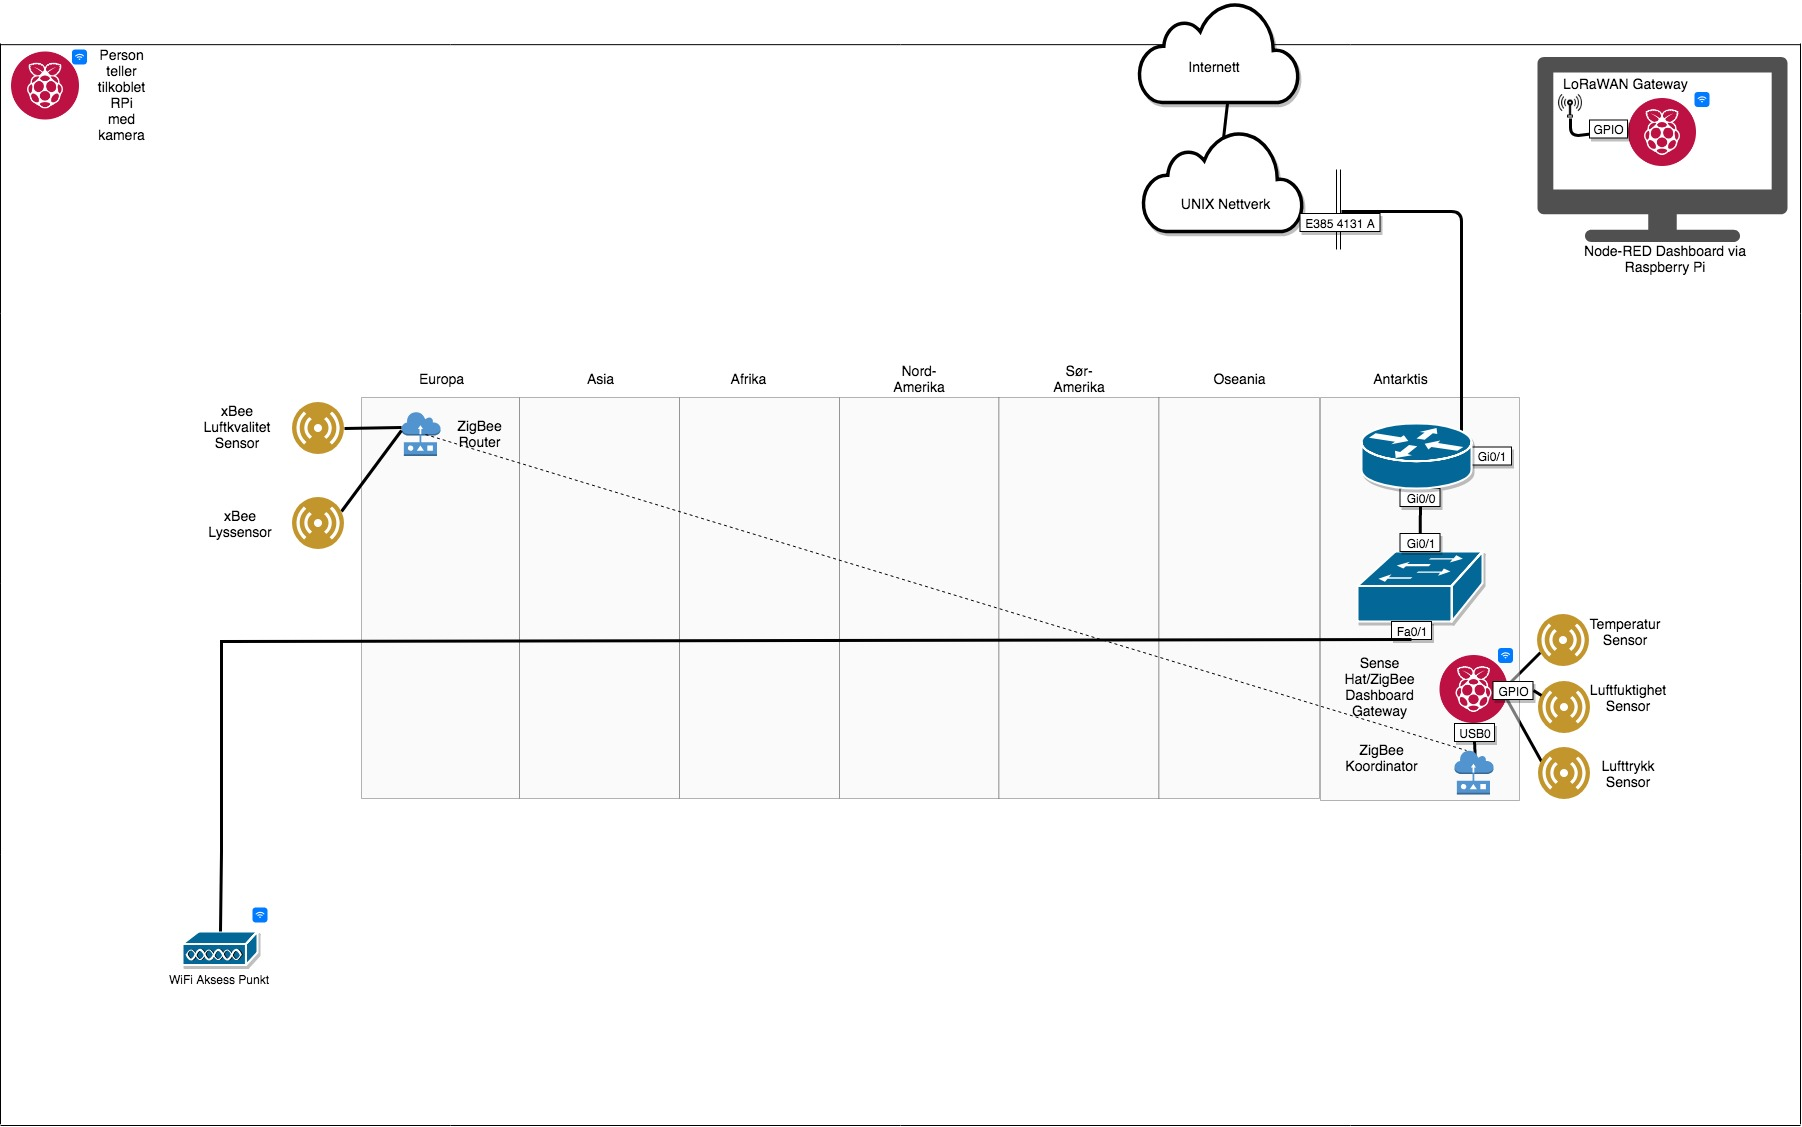
\includegraphics[width=0.9\textwidth]{lab}
 \caption{Oversikt over resultatet av IoT labratoriet}
\end{figure}


%----------------------------------------------------------------------------------------
%   TEORI SEKSJON
%----------------------------------------------------------------------------------------


\newpage
\section{Teori}

\subsection{Generelt}
For å gjøre rapporten så leselig som mulig, og for at den skal kunne brukes som dokumentasjon til IoT laboratoriet ser vi det nødvendig å ta en gjennomgang av temaet fra et teoretisk standpunkt først. I denne delen av rapporten vil vi derfor se på teknologiene som har blitt implementert på laboratoriet  før vi tar for oss opsettet og før vi ser utprøvelser av utstyret.

\subsection{Routere og Switcher}

\subsubsection{Routere}
En router er nettverksutstyr brukt til videresending av nettverkspakker, nettverkspakkene blir videresendt til et mottagende nettverk. Nettverkspakker kan være IP-Adresser, en unik identifikator som tildeles en enhet på et nettverk. For å bestemme hvor en pakke skal videresendes til brukes en routing tabell, en tabell på routeren som viser hvilke nettverk den er tilkoblet.

\subsubsection{Switcher}
En switch er en type nettverksutstyr som styrer trafikk på et nettverk. Formålet med en switch er å redusere unødvendig nettverkstrafikk, minske antall kollisjoner og øke hastigheten på nettverket.

\subsection{Raspberry Pi}
Når det kommer til valg av mikrodatamaskiner sto det i hovedsak mellom Raspberry Pi og Arduino. Vi endte til slutt opp med Raspberry Pi, det er flere grunner til dette, men først litt om selve Raspberry Pien vi har valgt.

\begin{figure}[h]
\centering
   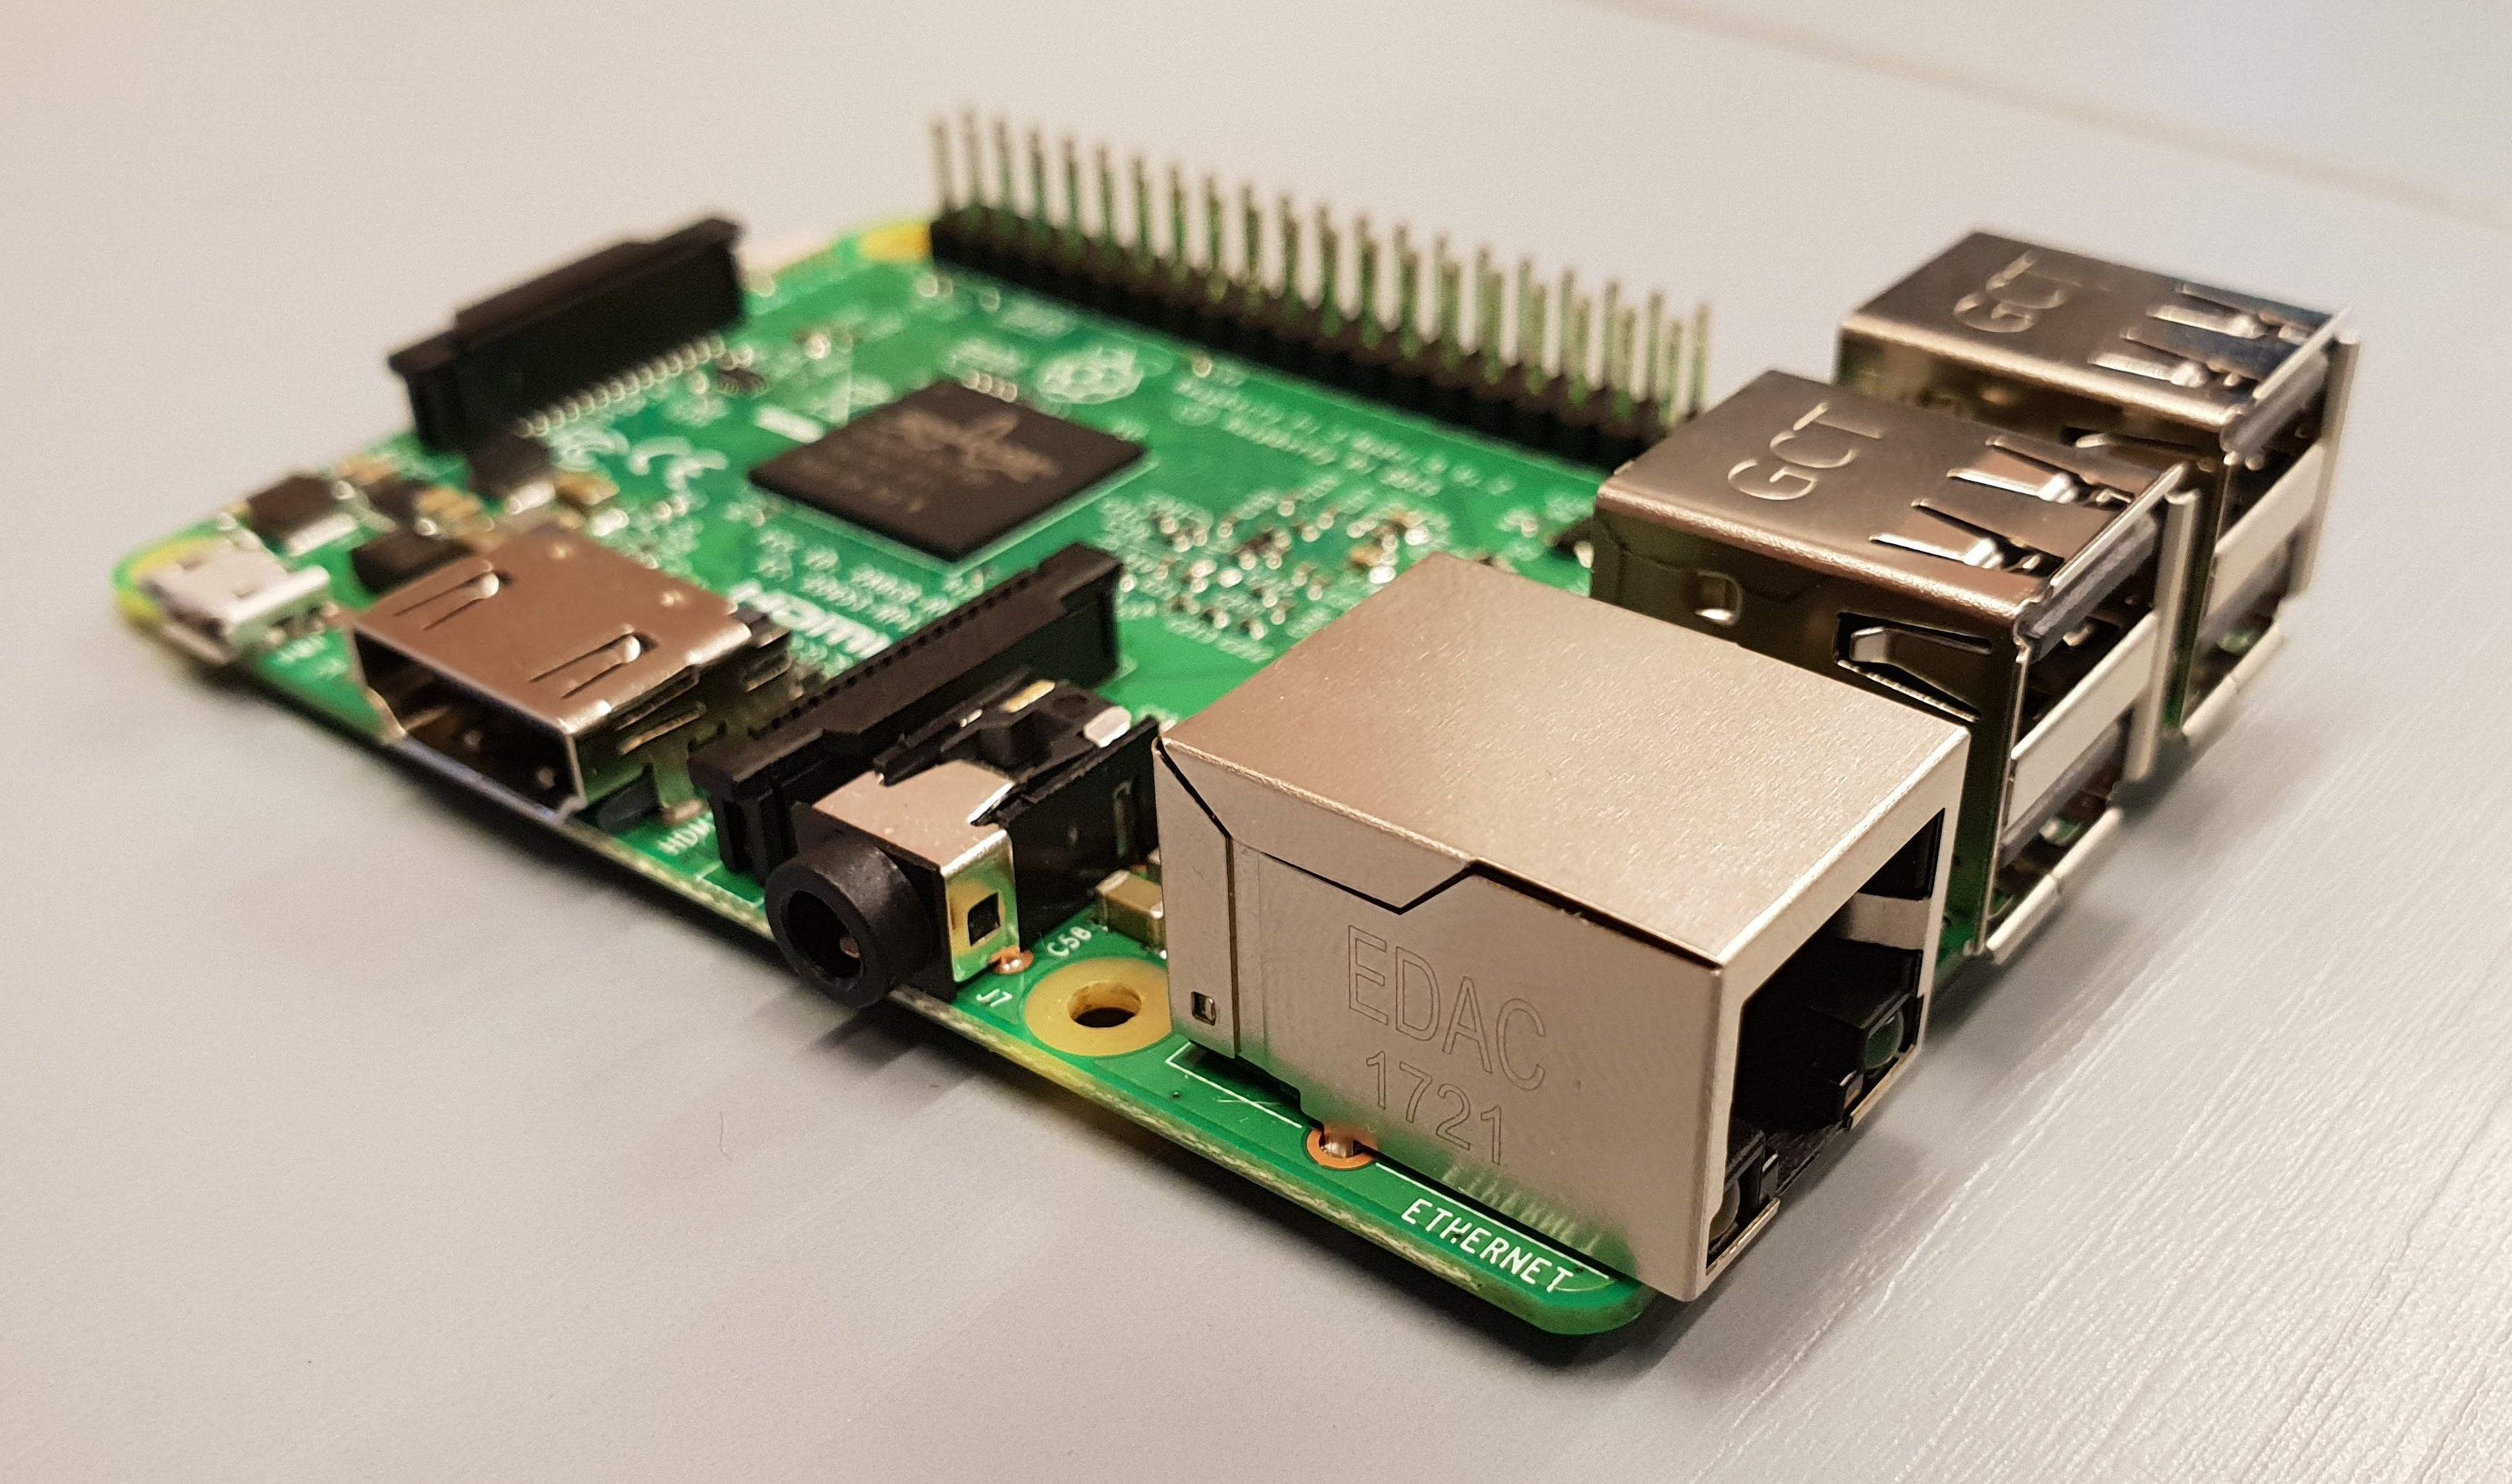
\includegraphics[width=1\textwidth]{RPi1}
\caption{Raspberry Pi Model 3B}
\end{figure}

En Raspberry Pi\cite{rpi} er en en liten datamaskin utviklet av det britiske selskapet Raspberry Pi Foundation. Den har et lite kretskort, ellers vil det meste avhenge av hvilken modell av Raspberry Pi man har. Vår modell er den nyeste, Raspberry Pi 3B, denne sto frem som det beste alternativet. Modell 3B har en Arm Cortex A7 er en 64-bits firekjernet prosessor, 1 Gigabit med RAM, 4 USB porter og 1 HDMI inngang. Dette gir den mange tilkoblingsmuligheter, og det vil være lett å ta i bruk da USB og HDMI er brukt ofte. I sær er det spesielt viktig med flere USB porter, dette gir mulighet for tilkobling av datamus og tastatur samt overføring av data på samme tid. Det ville vært mye vanskeligere å koble enheten til en skjerm dersom den for eksempel hadde en Displayport, da dette er en eldre teknologi. Det at en Raspberry Pi model 3B er den nyeste versjonen har vært viktig for oss da Tingenes Internett avdelingen i kommunikasjonsteknologi laboratoriet ikke burde være utdatert før det er ferdiglaget.

Raspberry Pi model 3B har mulighet for WiFi og Ethernet tilkobling til Internett. Det vil si at den er mer fleksibel i forhold til andre mikrodatamaskiner. Det er mye mer praktisk med en mikrodatamaskin som kan benytte seg av WiFi om man for eksempel skal bruke den til å hente og sende sensordata. Dersom man ønsker å bruke en Raspberry Pi til å sende data til en nettside for å monitorere temperatur, luftfuktighet og CO2 nivå på et serverrom vil det være en stor fordel å slippe å trekke kabler. WiFi gir også muligheten for rask sending av data, noe som er gunstig for en enhet som Raspberry Pi 3B som har muligheten til å tilkoble ting som krever mye båndbredde, som for eksempel kamera. 

En annen viktig grunn til å velge en Raspberry Pi er at den bruker lite strøm, som vil være nyttig for studenter. Dette kombinert med WiFi tilgang og mulighet for å nå enheten via SSH, gjør at man kan plassere den hvor som helst innen rekkevidden til WiFi signalet. Det gir muligheten til å koble til et batteri, for å være portabel. Dette åpner for at studenter vil kunne være kreative i implementeringen av tingenes internett.

I tillegg til å støtte Wi-Fi 802.11b/g/n støtter også modell 3B Bluetooth 4.1. Det er aktuelt da det finnes et stort marked for sensorer og “ting” som kommuniserer med Bluetooth. Et eksempel er Fitbit, som har et stort utviklermiljø og har flere tjenester som tilrettelegger for egen utvikling av programvare som kommuniserer med Bluetooth.

Raspberry PI støtter flere Linux baserte operativsystemer og Windows 10 IoT Core. Sistnevnte er en nedstrippet versjon av Windows som er optimalisert til å kjøre på mindre enheter.   Windows 10 IoT Core er designet med IoT i tankene og er også betydelig lettere å tilkoble til Microsoft Azure IoT Hub\cite{azureiothub} enn Linux baserte operativsystemer.

\subsubsection{Raspberry Pi Sense Hat}
Raspberry Pi Sense Hat er et tilleggskort for Raspberry Pi, kortet festes til GPIO pinnene og skrus fast med medfølgende skruer. Kortet er laget som en del av Astro Pi oppdraget, og en Raspberry Pi med tilkoblet Sense Hat er sendt ut i verdensrommet. Denne kjører studenters små programmer på den internasjonale romstasjonen (ISS). Kortet har et medfølgende Python bibliotek for enkel implementasjon. Raspberry Pi Sense Hat har følgende funksjonaliteter:

\begin{itemize}
	\item Temperaturmåler
	\item Gyroskop	
	\item 8x8 LED matrise
	\item Akselerometer
	\item Joystick
	\item Barometer
	\item Luftfuktighet
	\item Magnometer
\end{itemize}


\subsection{WiFi}
WiFi er en teknologi for trådløs lokalområde nettverking med enheter som er basert på IEEE 802.11 standarden. WiFi er en av de mest utbredte teknologiene for trådløs nettverking og er noe de fleste populære enheter har mulighet for å bruke. WiFi kan sende relativt stor mengde data over kort tid, noe som krever en del strøm. Og er veldig nyttig i IoT enheter som trenger å sende stor mengde data og har mulighet for konstant strømtilkobling, som for eksempel et overvåkningskamera.

WiFi har en rekkevidde på ca. 20 meter innendørs, og en litt større rekkevidde utendørs. WiFi utnytter for det meste 2.4 GHz og 5 GHz radio bølgefrekvens. Siden WiFi er tilgjengelig for alle som er innenfor rekkevidden for aksesspunktet så er sikkerhet noe som er veldig viktig i et slikt nettverk.
Det finnes mange WiFi teknologier, man har 802.11a sender på 5GHz og kan sende 54 MB med data per sekund. 802.11b er den seneste men minst kostbare standarden, den sender over 2.4 GHz og kan sende 11 MB data per sekund. 802.11g sender også over 2.4 GHz men er mye kjappere med en datarate på 54 MB i sekundet. 802.11n er den mest tilgjengelige standardene og er kompatibel med både a,b og g. Den har bedre data rate og rekkevidde enn tidligere standarder. 802.11n kan sende opp til 140 MB/s og kan sende opp til fire strømmer med data samtidig. For øyeblikket er 802.11ac under arbeid hos IEEE men noen enheter som støtter det er allerede på markedet. 802.11ac kan sende opp til 450MB/s over både 5GHz og 2.4 GHz båndbredde.


\begin{figure}[h!]
\centering
    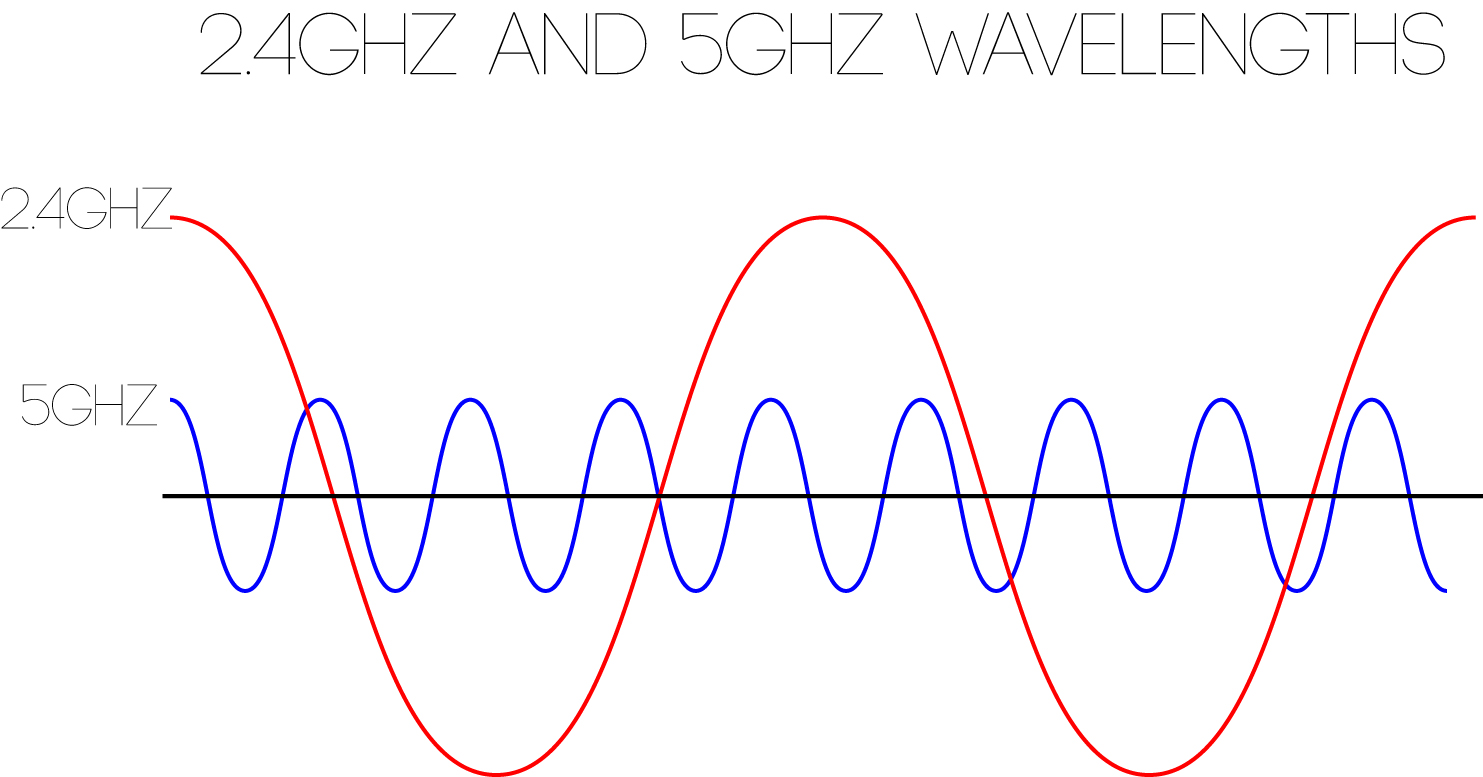
\includegraphics[width=0.9\textwidth]{wavlengths}
\caption{Illustrasjon av forskjellen på 2.4GHz og 5 GHz\cite{wavlengths} }
\end{figure}

\newpage
\subsection{ZigBee}
Denne delen vil ta for seg teori rundt ZigBee og XBee modulene som konfigurasjon av moduler, oppbygging av og de forskjellige rollene i et ZigBee nettverk, hvordan adressering og identifisering blir gjort.  All programmering, bruk og tilkoblinger av sensorer som er utført i oppgaven er dokumentert i eget avsnitt senere i rapporten. La oss først avklare forskjellen mellom ZigBee og XBee.

\begin{itemize}
	\item ZigBee er en lav kost, to veis trådløs standard som er bygget over 802.15.4 standarden. Det er altså den øverste delen av protokoll stacken i figuren under
	\item XBee er en modul med blant annet innebygd ZigBee protokoll. Det er også en fastsatt form factor med tanke på utseende og oppsett på av de ulike komponentene på brikken som grensesnitt og pinner
\end{itemize}

I denne rapporten vil XBee som regel referere til den fysiske modulen mens ZigBee vil hovedsakelig omhandle teknologien i de 2 øverste lagene, altså nettverk og applikasjon.

\begin{figure}[h!]
 \centering
     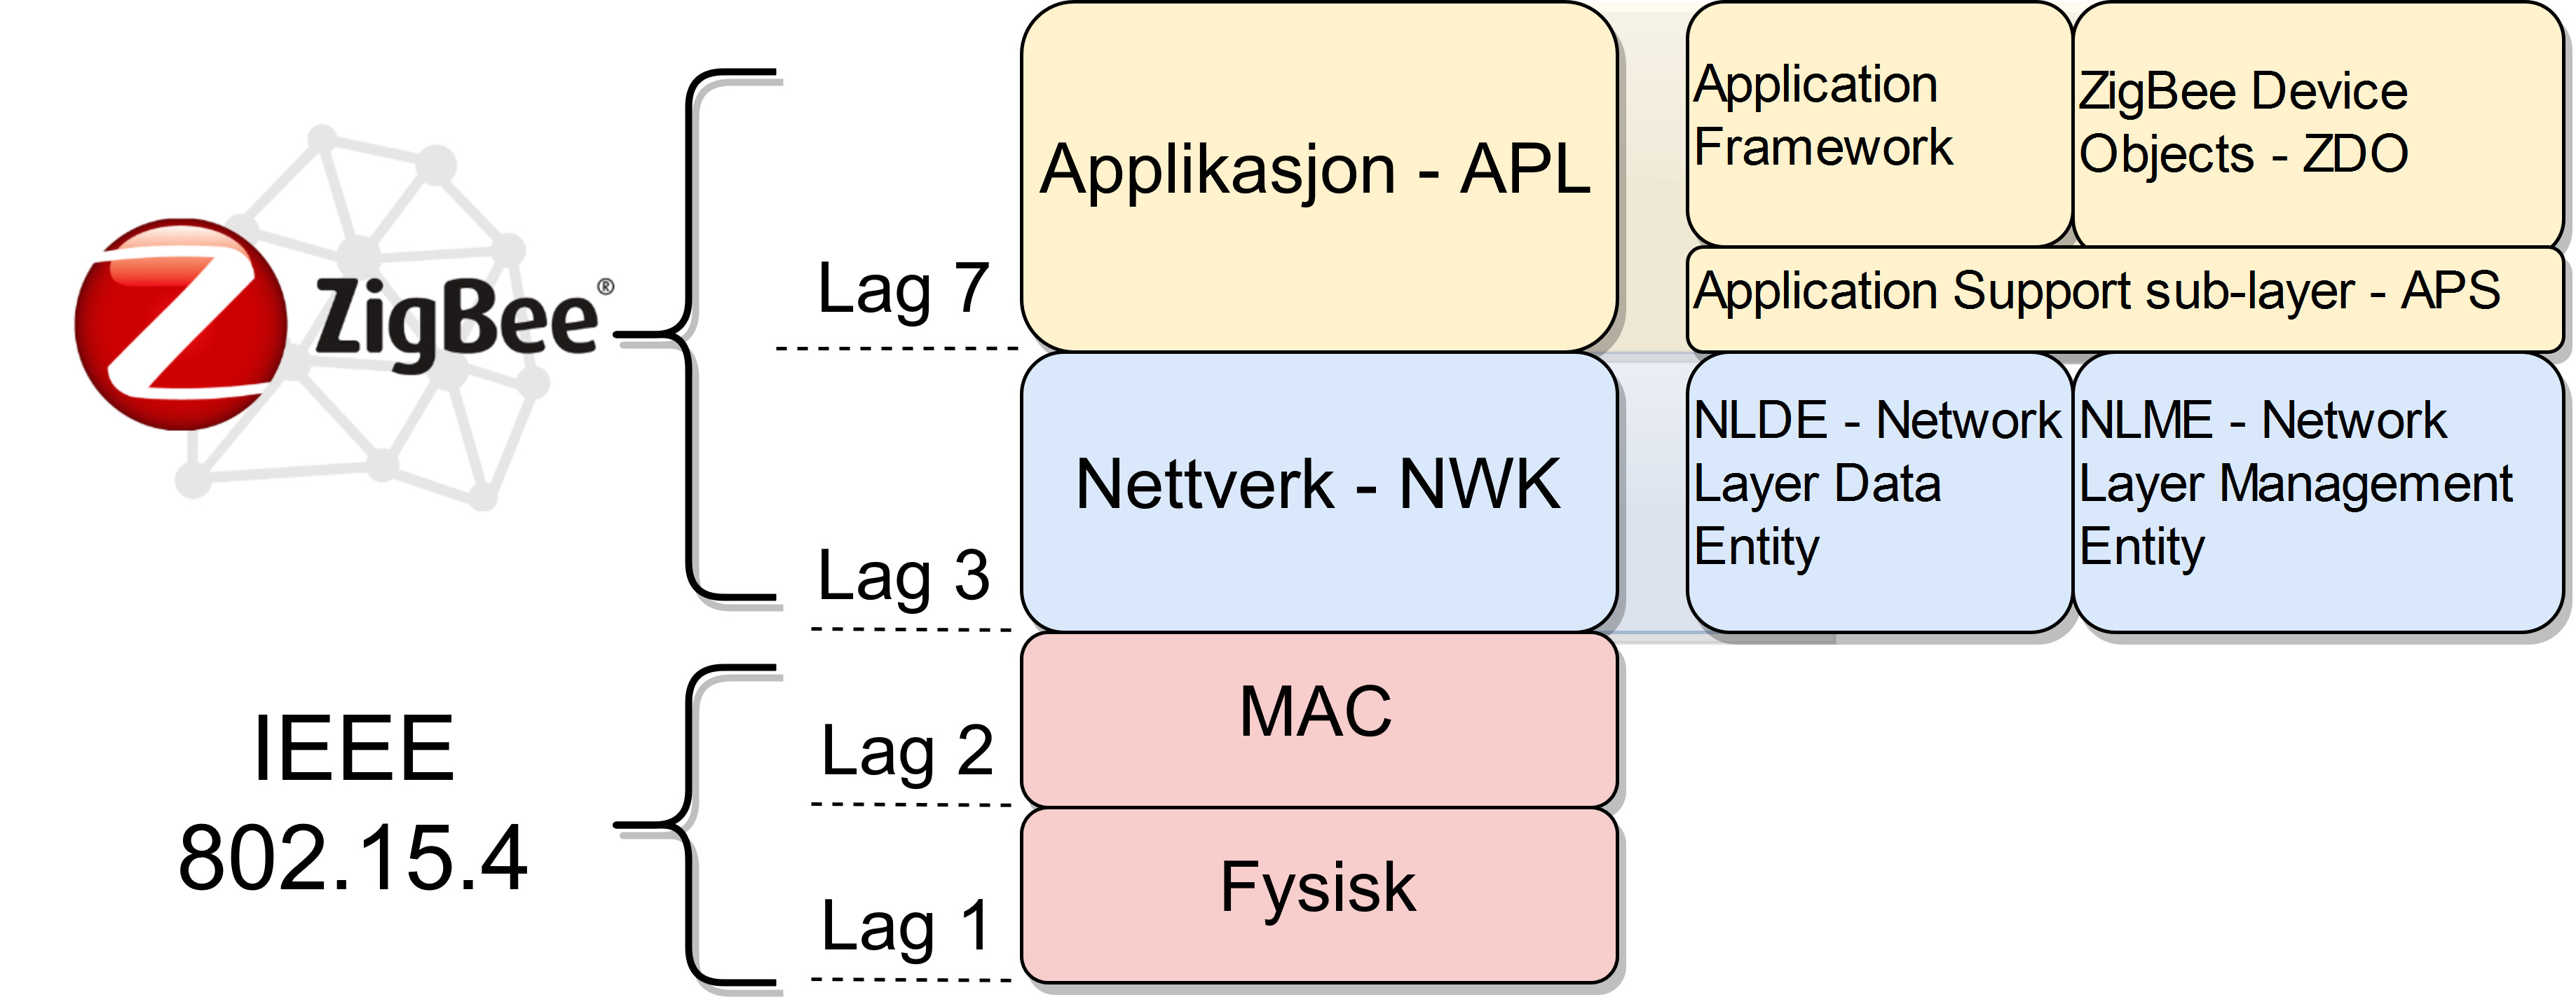
\includegraphics[width=0.9\textwidth]{zigbeeosimodellv2}
 \caption{Overblikk over de forskjellige lagene i ZigBee modellen og dens funksjoner.}
\end{figure}

\subsubsection{Nettverk laget - NWK}
Dette laget håndterer adressering, ruting, nettverksstruktur og deler av sikkerheten. Den passer på at underliggende lag, IEEE 802.15.4 opererer som ønsket og står videre for grensesnitt videre opp mot applikasjons laget. Data opp mot applikasjon laget kan deles opp i to entiteter, NLDE (Network Layer Data Entity) og NLME (Network Layer Management Entity). NLDE sørger for transport av data mellom 2 eller flere enheter.  Dette kan for eksempel være verdier fra sensor. NLME sender pakker til ZigBee Device Ojects og inneholder instruksjoner rundt styring og koordinering i nettverket og dens noder. Begge disse går opp til applikasjonslaget via Application Support sub-layer (APS).

\subsubsection{Applikasjon - APS}

\subsubsection{Trådløs og seriell kommunikasjon}
XBee enheter kan ta i bruk trådløs eller seriell kommunikasjon for overføring av data. Selv om det eksisterer andre protokoller, er det vanligst å benytte ZigBee for sending av data på nettverket. Det er også mulig å konfigurere ZigBee nettverk for trådløs sending av data gjennom MQTT-SN, en modifisert versjon av den populære IoT protokollen MQTT. MQTT vil bli nærmere beskrevet i et senere avsnitt. Seriell kommunikasjon benyttes som regel under konfigurering av modulen og innsamling av data fra en slutt enhet som eksempelvis en sensor

\subsubsection{Adressering}
En XBee enhet har forskjellige måter å identifiseres  hvor det finnes 64-bit-, 16-bit- og Node- Identifikator. 64-bits identifikatoren er global unik og vil som regel være MAC-adressen. Denne vil være delt opp i to 32-bits deler, SH og SL, som står for Serial Number High og Serial Number Low. SL delen som består av de siste 32 bit vil følgelig være unik ettersom den består av NIC Network Interface Controller) delen av MAC adressen. 


\begin{figure}[h!]
\centering
   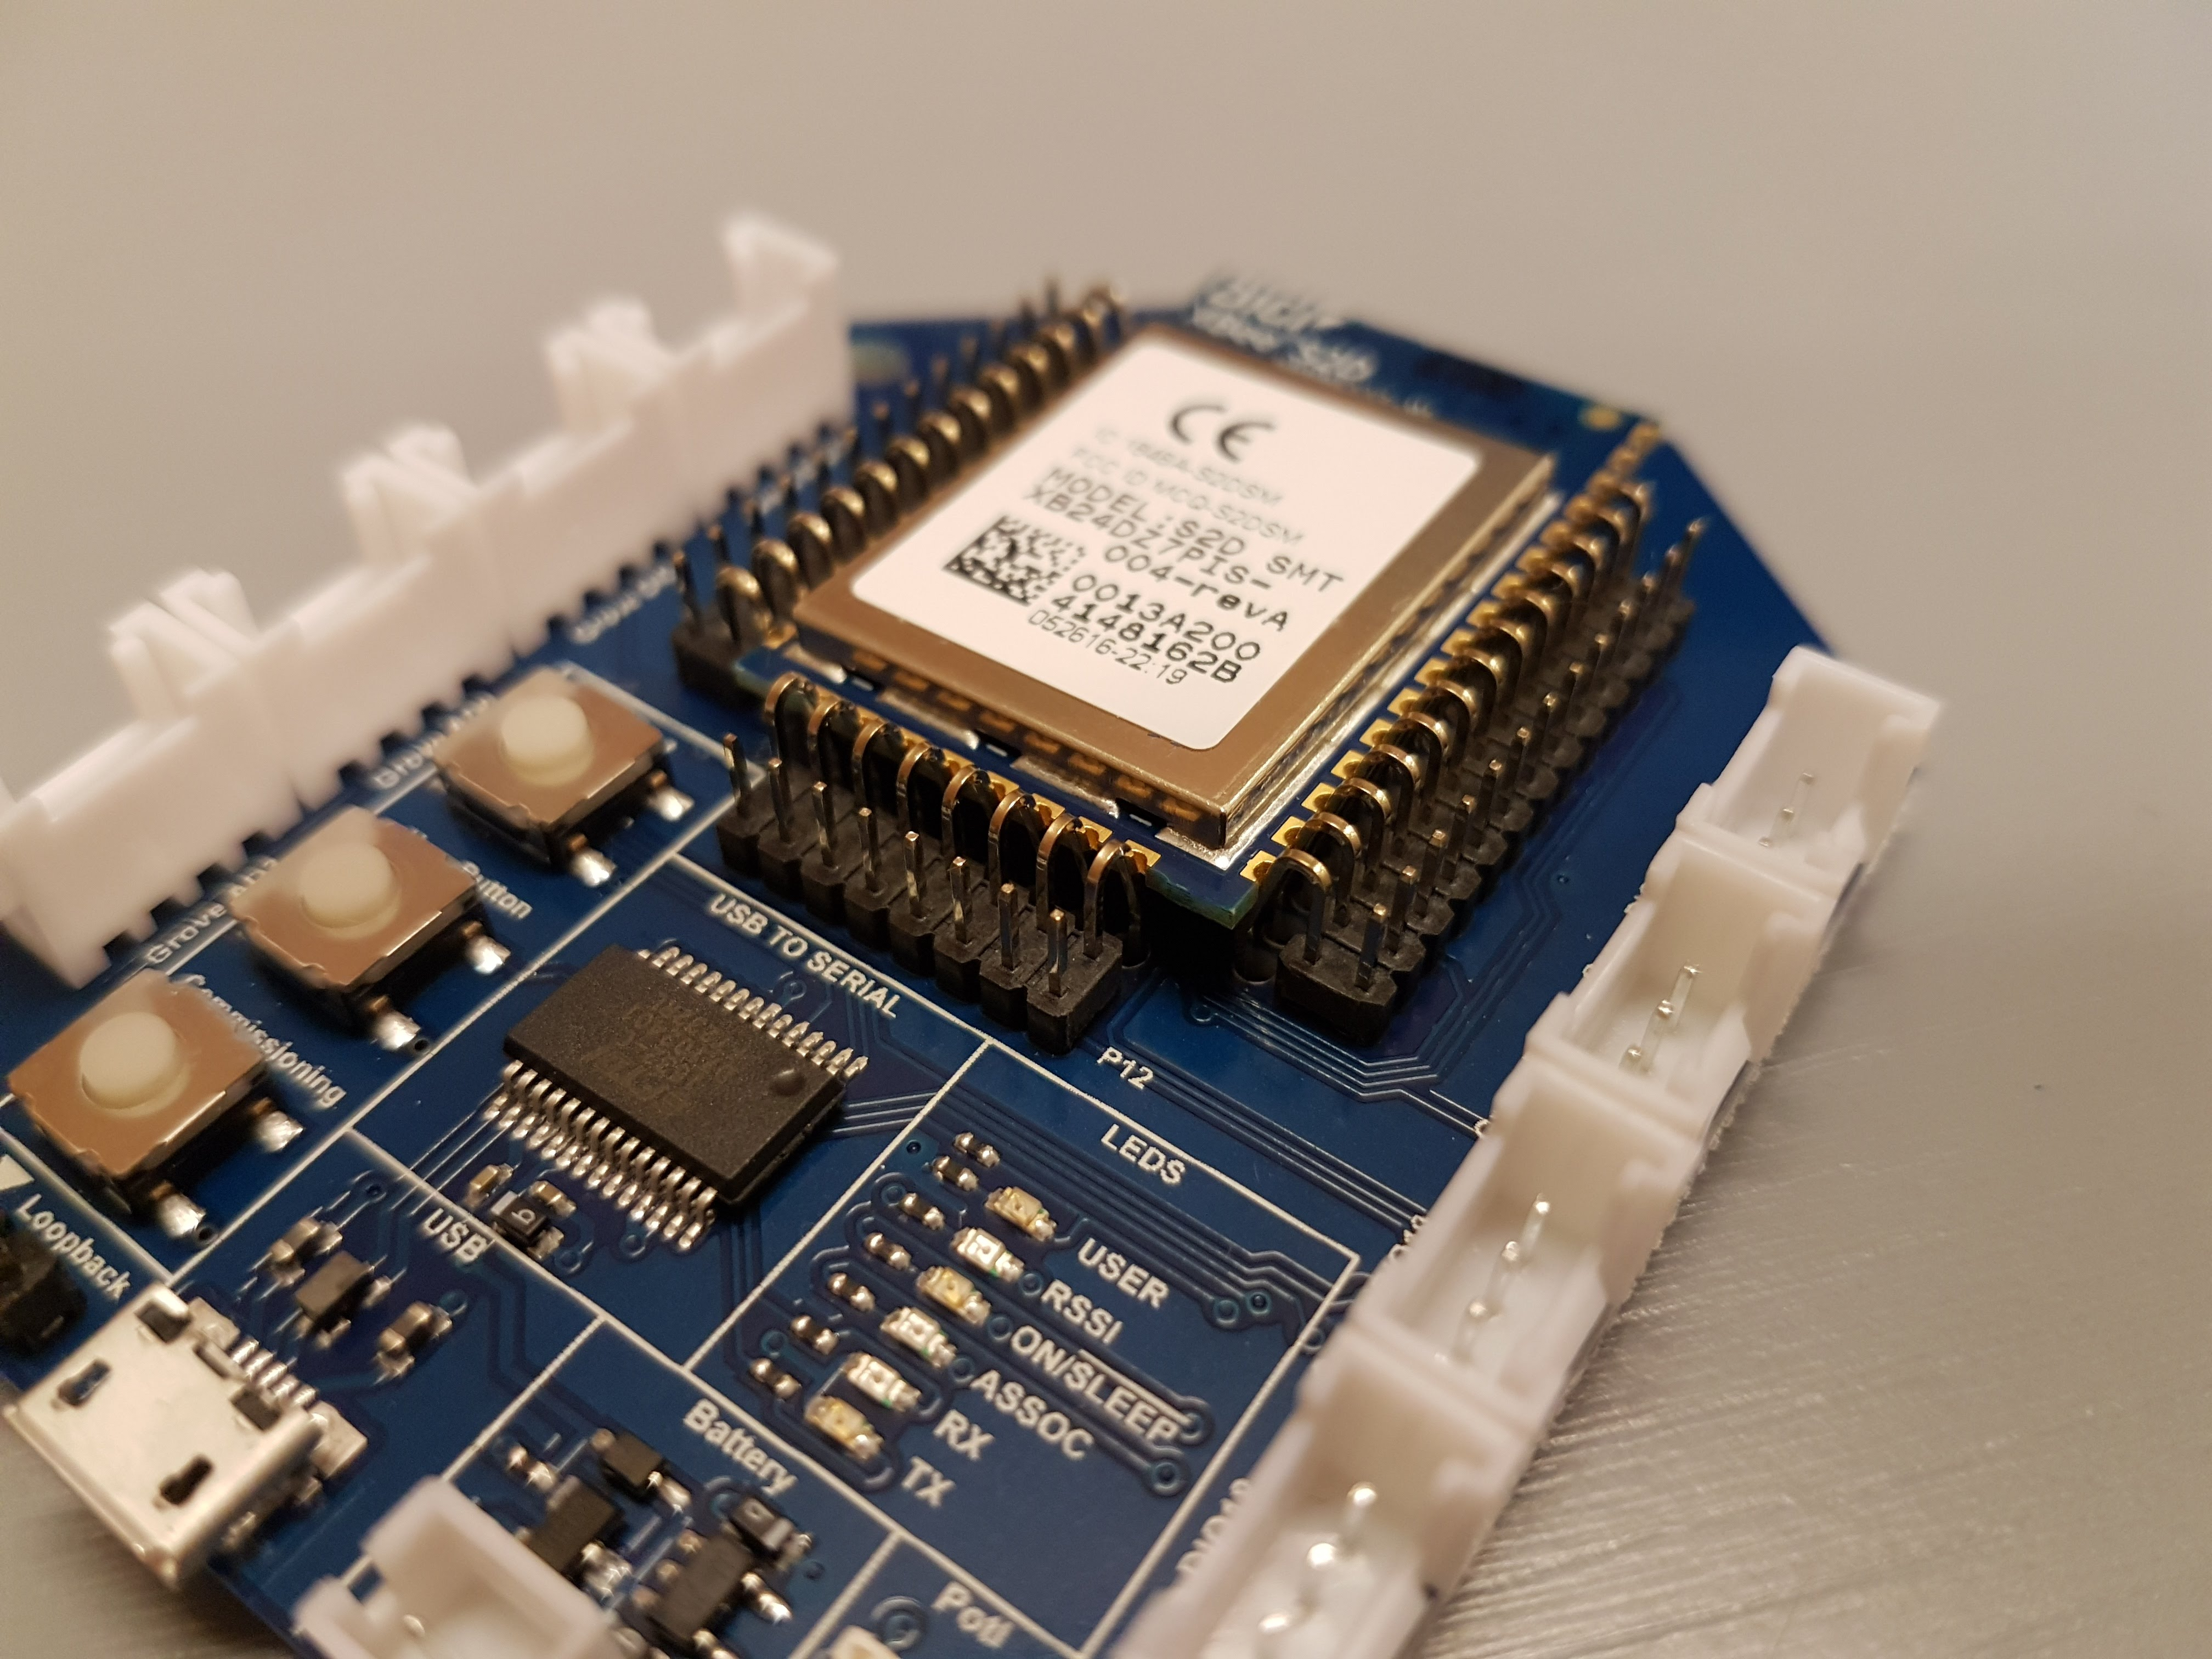
\includegraphics[width=0.5\textwidth]{xbeekort}
\caption{xBee Development Board}
\end{figure}

Hver enhet vil også ha en tilfeldig valgt nettverksadresse på 16 bit som den vil få tildelt av enten en router eller koordinator når den kobles til nettverket. Nettverksadresse er satt til FFFF når xBee modulen ikke er tilkoblet noe nett. 0000 er reservert koordinator noden. Ettersom det er tilfeldig valgt verdi innad i nettverket kan den ikke garanteres å være global unik men vil være unik innad i nettverket. Dette er noe router og koordinator sørger for. Det er hovedsakelig denne adressen nettverket bruker som identifikator på de forskjellige noder noe som er naturlig da det medfører mindre overhead enn 64 bit adressen samtidig som den garanter unikhet.  På mange måter kan nettverksadressen sammenlignes med en ip adresse.

Til slutt har en node identifikator som kan bestå av ASCII tegn og er tenkt å være en lett leselig måte å identifisere noden for mennesker. Denne trenger ikke være unik ettersom ZigBee nettverket ikke benytter verdien til noen form for routing eller koordinering. 


\begin{figure}[h!]
\centering
   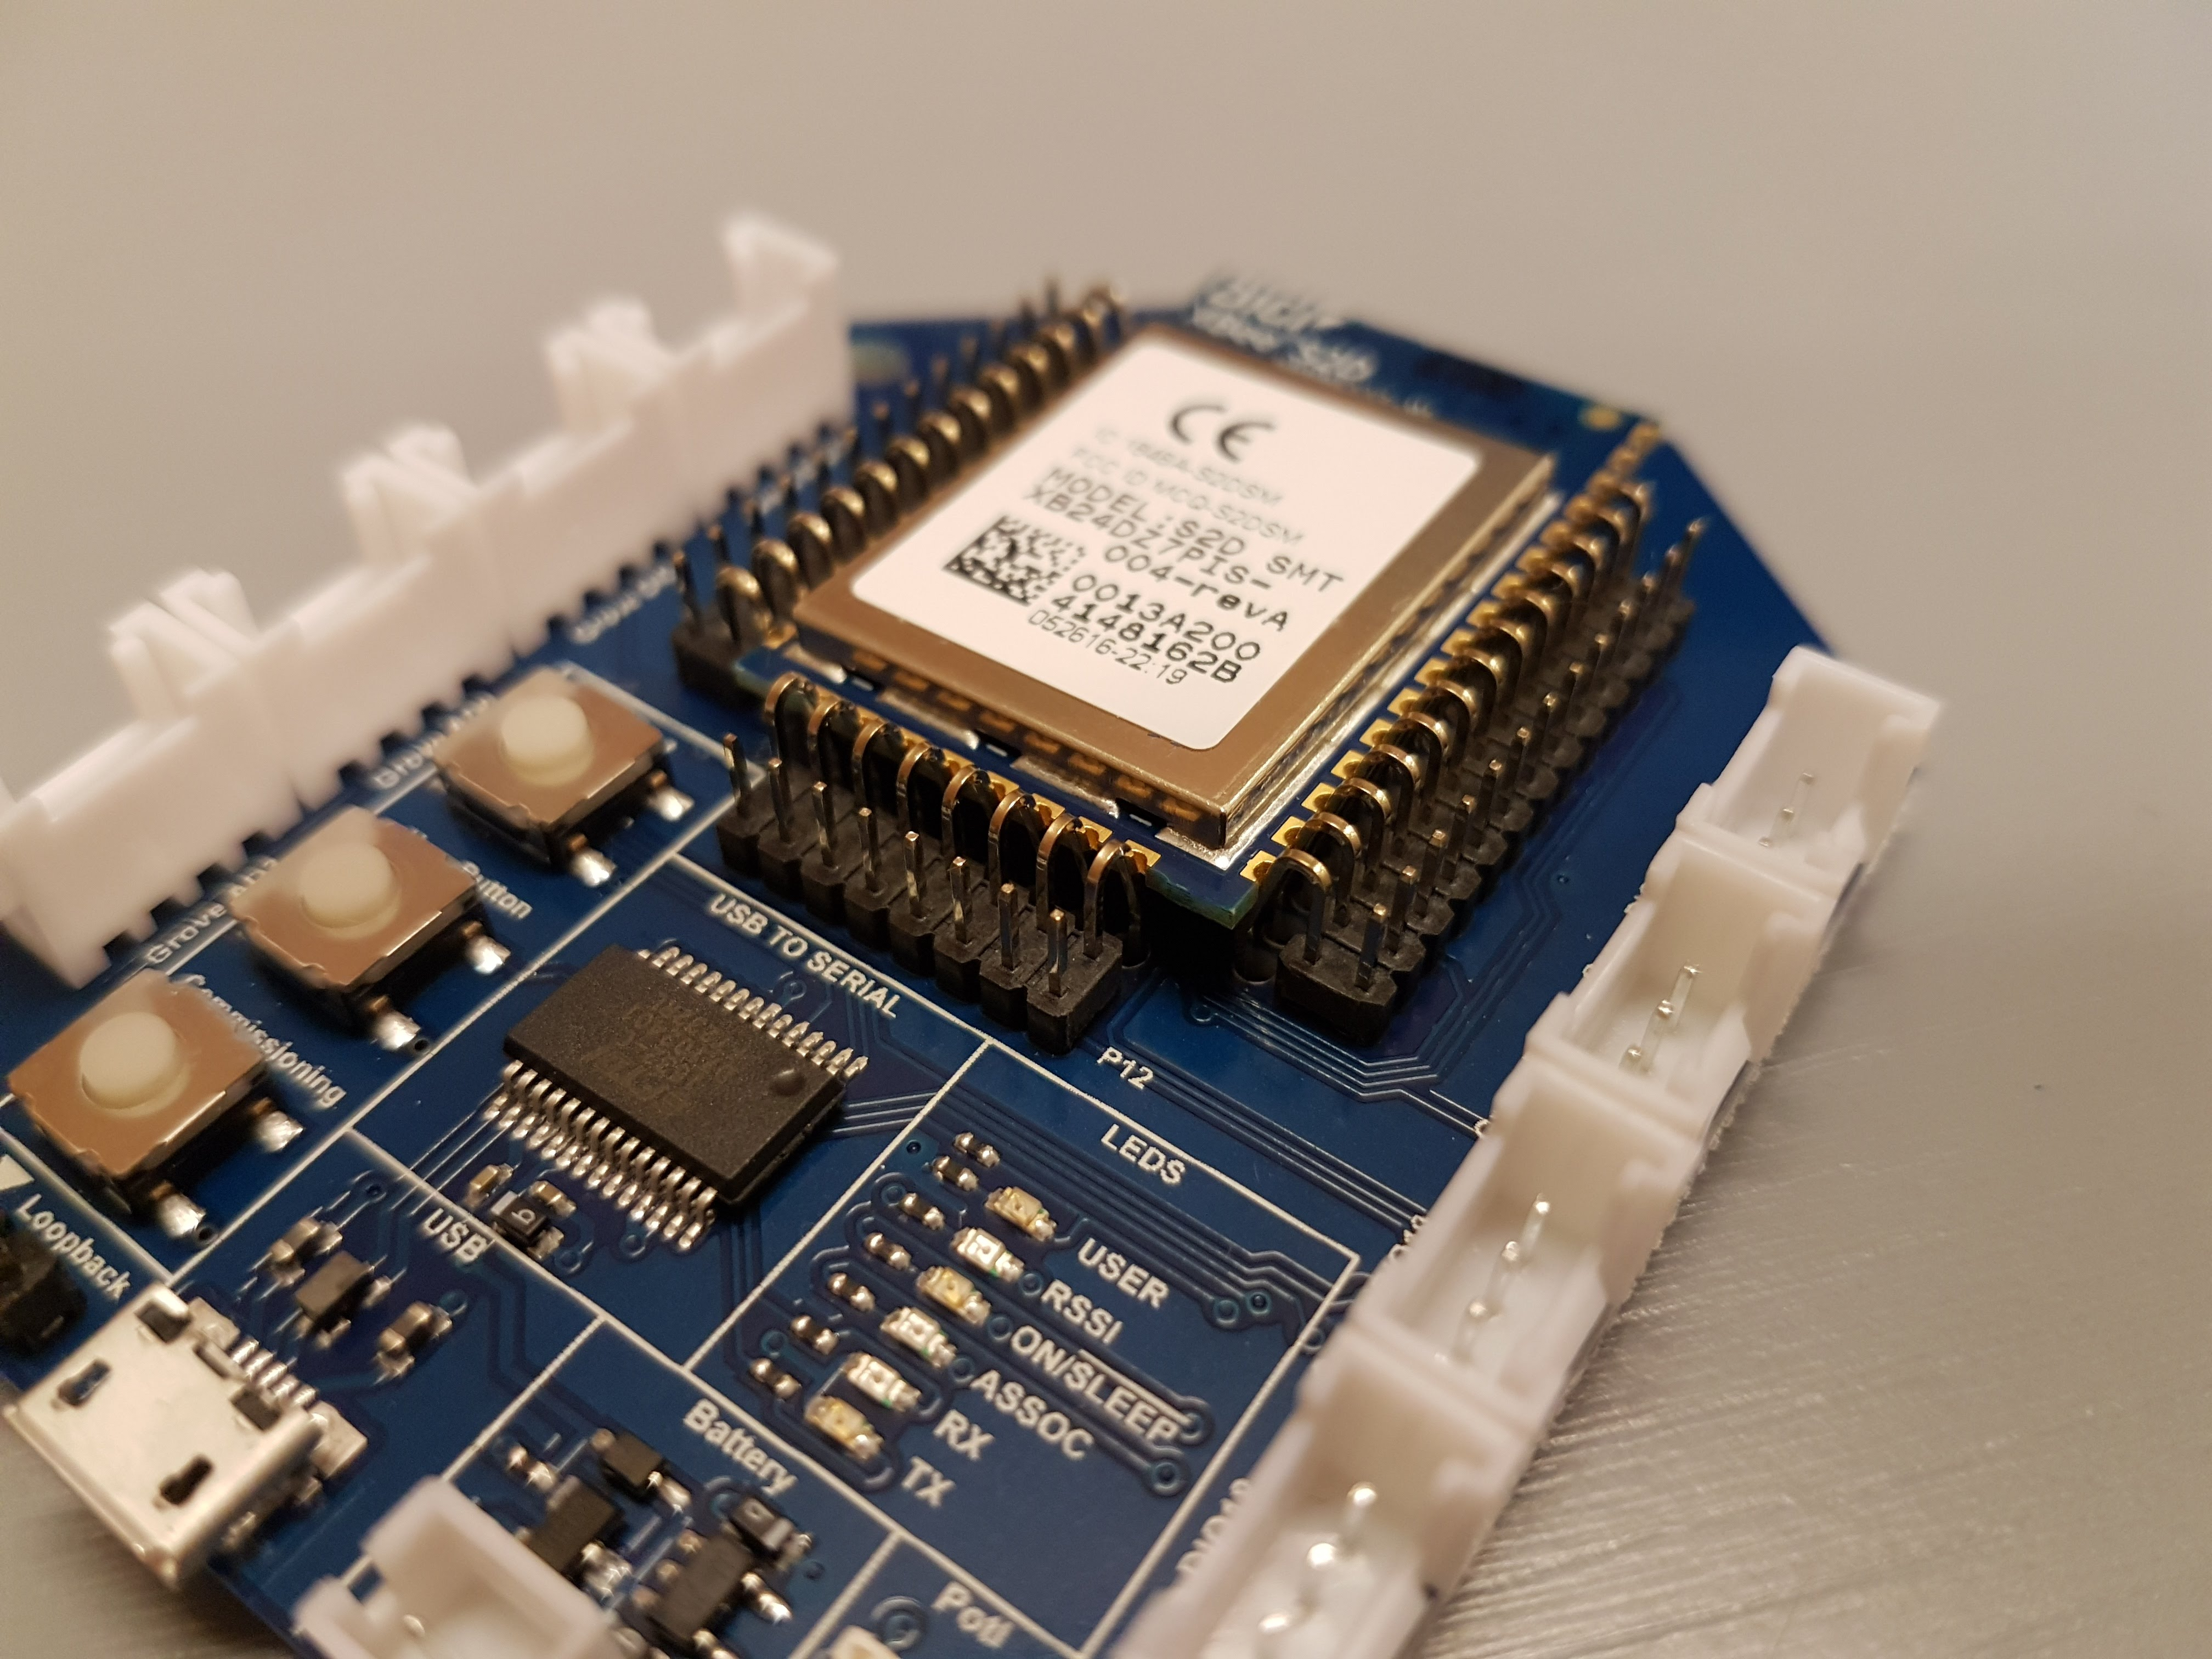
\includegraphics[width=0.5\textwidth]{xbeekort}
\caption{xBee Development Board}
\end{figure}

\subsubsection{Wireless Personal Area Network - WPAN}
Ett ZigBee nettverk er hva en kaller et WPAN eller Wireless Personal Area Network. Med dette menes et trådløst nettverk av enheter over et mindre område som kan kommunisere med hverandre, gjerne i form av et mesh nettverket, uavhengig av en gateway. Et ZigBee nettverk vil ha en PAN ID på 16 Bit for å identifisere nettverket. Det kan sammenlignes med en SSiD i WiFi verden men til forskjell fra SSID er det ikke mulig for to nettverk med identisk PAN ID å eksistere sammen. Ved konflikter kan EPAN ID - Extended Personal Area Network ID benyttes. Denne er på 64 bit og skal sikre unikhet. Dette er derimot ikke garantert på samme måte som 64-bit node adressen er. Dette er da EPAN ID blir valgt uten noe fastsatt standard til som ved MAC adressering. Til vanlig vil PAN brukes framfor EPAN da førstnevnte gir lavere overhead.



\subsubsection{XBee og Søvnmodus}
Strøm konsumering er et viktig aspekt av IoT da en enhet ikke nødvendigvis har tilgang til strømnettet og er avhengig av batteri. XBee sluttnoder kan putte seg selv inn i en midlertidig søvnmodus hvor de bruker ekstremt lite strøm. Under søvnmodus er modulen nesten helt skrudd av og vil ikke kunne ta inn eller sende data før den våkner opp. Router og koordinator noder kan ikke settes i søvnmodus. La oss anta at batteritid med en XBee uten å ha søvnsyklus er på en dag. Men om man da setter modulen inn i en søvnsyklus hvor den sover i 1 sekund, og våkner i 1 sekund, så har man allerede doblet batteritiden. Setter man den til å syklisk sove i 99 sekunder, og våkne for å sende data i 1 sekund, så har man gått fra 1 dag med batteritid, til 100 dager. Det er lett så hvor kraftig dette kan være med tanke på levetid. 

\begin{figure}[h!]
\centering
   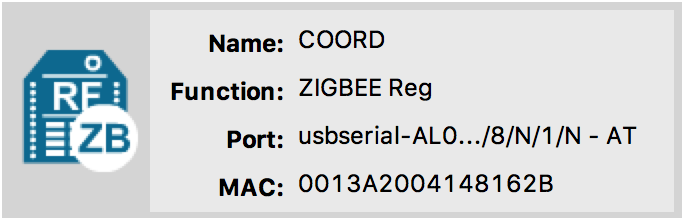
\includegraphics[width=0.4\textwidth]{xctucoord}
\caption{Koordinator tilkoblet en datamaskin klar for konfigurering i XCTU}
\end{figure}

Det finnes tre forskjellige typer søvnmodus:
\begin{enumerate}
	\item Pin sleep (SM=1) - Lar en ekstern mikrokontroller kunne bestemme når XBee modulen skal sove og når den burde våkne ved å kontrollere Sleep RQ pin (pin 9). Når denne pinen går høyt ( får inn 3.3 volt), vil modulen gjøre seg ferdig med siste operasjon og gå inn i søvnmodus, den vil så våkne når pin 9 går lavt (0 volt inn)
	\item Cyclic Sleep (SM=4) - Setter XBee modulen til å sove i bestemte sykluser. Når den våkner så vil den sende data fra en eventuell tilkoblet sensor, spørre koordinator etter beskjeder, så gå tilbake i søvn.
	\item Cyclic sleep with pin wake-up (SM=5) - Denne modusen fungerer som en blanding av de to tidligere modusene. Modulen vil gå i søvn i bestemte intervaller, men med pin wake-up så åpner det for muligheten til å eksternt be den våkne.
\end{enumerate}



\subsection{LoRaWAN}
I denne delen skal vi se nærmere på LoRaWAN, dens fordeler, ulemper og hvor det er best å implementere det.

LoRaWAN er en nettverksprotokoll som er en LPWAN protokoll som er designet for å være ekstremt kostnadsfri over lange avstander, etter teori så kan LoRaWAN sende signaler opp til 700km(?), men i realitet, med tanke på forskjellige forstyrrelser som luft, trær, bygninger, og til og med bakken selv, så vil rekkevidden nå opp til 10 km. Protokollen utnytter ekstremt lav båndbredde for å kunne være så kostnadsfri og enda sende signal over store avstander. Mens en node som sender data over WiFi har levetid på noen dager, så vil en node som sender data over LoRa kunne leve i flere år.

Dette er nok noe av grunnen til at Stavanger smartby har valgt å implementere LoRaWAN for sine noder i Stavanger. Med tanke på at dette implementeres her i Stavanger, så ser vi på det som veldig hensiktsmessig for studenter ved UiS å ha kjennskap til protokollen.

LoRaWAN bruker så lav båndbredde, at istedenfor som Wifi å sende tusenvis av bits, så sender denne protokollen ti-talls bits. Data raten til LoRaWAN er definert å ligge mellom 300 bps - 5.5 kbps. Noe som i praksis er seinere enn en dyktig morsekode operatør. Så LoRa er ikke en protokoll som man sender store kritiske mengder data over, men brukes heller til noder som ikke har så høye båndbreddekrav. Så man kobler ikke et livestream kamera opp og forventer at LoRa skal kunne gi deg bra kvalitet og seamless streaming. Dette er heller ment for å sende temperatur, lufttrykk eller annen ikke kritisk, lav båndbredde data.
Siden LoRa ikke har lov til å bruke mer enn 1 prosent av dens potensiale strømforsyning så har den ikke så veldig god evne til å penetrere forskjellige materialer.


LoRa støtter bi-direksjonal kommunikasjon, stor mobilitet, og lokalisasjon (dette er i debatt, ettersom det kan være veldig vanskelig å lokalisere noder mtp hvordan teknologien fungerer - https://www.link-labs.com/blog/lora-localization)
Protokollen opererer innen lisens-frie ISM bands i forskjellige regioner, 433 Mhz i Asia, 915 Mhz i USA, og 868Mhz i Europa. Å operere utenfor disse Mhz er ulovlig, så å bestille en LoRaWAN modul i rett Mhz var en av tingene som måtte vurderes når vi bestilte utstyr.  Vi valgte å gå for en HAT som settes på en Raspberry Pi fordi dette var billig, og lett for studenter å kunne sette opp.

Protokollen lever mellom lag to (data link) og lag tre (nettverk) i OSI modellen:
\\
LoRaWAN frekvenstabell:
\begin{table}[h!]
\centering
\caption{LoRaWAN frekvenstabell}
\label{lorawan-frekvenstabell}
	\begin{tabular}{|l|l|}
	\hline
		\textbf{Land/Region} &  \textbf{Frekvens}\\ \hline
		Europa &  863-870 MHz\\ \hline
		USA &  902-928 MHz\\ \hline
		Kina &  779-787 MHz\\ \hline
		Australia &  915-928 MHz\\ \hline
	\end{tabular}
\end{table}


\subsection{Bluetooth}
Bluetooth er en trådløs dataoverføring protokoll for kommunikasjon over korte distanser i et personlig datanett. Det ble oppfunnet av Ericsson i 1994 og ble originalt designet som et trådløst alternativ til RS-232 kabler. IEEE har standardisert Bluetooth som IEEE 802.15.1. Bluetooth overføring har en laver overføringshastighet enn WiFi, og kan ikke brukes for strømming av video. Foruten strømming av video kan Bluetooth brukes til sending av de fleste typer data som blir innhentet i et IoT laboratorium. En ulempe med Bluetooth er at strømmforbruket er høyt i forhold til andre teknologier, dette er et problem som er i ferd med å opphøre dat det utvikles nye versjoner av Bluetooth. Bluetooth 5 er fokusert mot IoT, og ble lansert i April 2017. Bluetooth 5 har blit tatt i bruk av flere store smart telefon produsernter som Apple og Samsung, og teknologien blir stadig mer tatt ibruk. Fordelene med Bluetooth 5  er raskere overføringshastighet, lenger rekkevidde og lavere strømmforbruk enn forgjengeren Bluetooth 4.2.

De store salgs punktene for Bluetooth er at det er trådløst, billig, og har automatisk tilkobling. Bluetooth krever “agreement” på det fysiske nivå - radiofrekvens standard - og på protokoll nivå, hvor noder må si seg enig i når bits blir sendt, hvor mange som skal bli sendt, og hvordan partene i samtalen kan være sikre på at meldingen som er mottatt er den samme som den som ble sendt.

Bluetooth nettverking sender data via low-power radio bølger. Det kommuniserer på en frekvens mellom 2.402 GHz og 2.480 GHz.  En av måtene Bluetooth forhindrer å forstyrre andre systemer er ved å sende ut veldig svake signaler på rundt 1 milliwatt. Dette er lavt med tanke på at en kraftig telefon kan sende signaler opp til 3 watt. Denne lave strømmen begrenser rekkevidden til Bluetooth til 10 meter. Bluetooth kan koble opp til åtte enheter samtidig, man ville trodd at om alle disse enhetene var koblet sammen i en 10 meters rekkevidde at de ville forstyrret hverandre, men det er usannsynlig. Bluetooth bruker en teknikk som kalles “spread-spectrum frequency hopping”. I denne teknikken så vil en enhet bruke 79 individuelle tilfeldig valgte frekvenser innen en gitt rekkevidde. Bluetooth endrer disse frekvensene 1600 ganger i sekundet, noe som gjør det usannsynlig at to sendere vil være på samme frekvens samtidig. Og selv om de ender opp på samme frekvens, så vil dette være i en så kort tid at det vil ikke spille en stor rolle.



\subsection{Mobilnett}
Mobile nettverk er noe som har blitt ekstremt utbredt etter smarttelefonen ble mer og mer populær. Brukere sin mulighet for å sjekke internett og sende epost via telefonen begynte å drive kravene for data-kapasitet over nettverk lenger og lenger. Vi gikk ifra 2G på 80-tallet, som kunne bære stemme trafikk, til 3G i tidlig 2000 som kunne bære stemme, email, tekst, og treigt Internett. I dag har vi kommet til 4G+ generasjonen. Mobile nettverk kan sende data over forskjellige frekvenser, men det er mest hensiktsmessig å holde seg rundt lavere frekvenser grunnet disse frekvensene sin mulighet til å sende data over lengre avstander, og deres større potensiale for å kunne nå enheter som ligger bak f.eks murvegger.

4G er en full-IP standard. Noe som betyr at det bruker full IP adressering for all data, til og med stemme-data, noe som 3G ikke gjør.

4G ble egentlig kalt 3.5G, 3.9G eller 3G+, men etter mye press fra store selskaper's markedsføringsavdelinger har det nå fått det nye navnet 4G for å kunne selge mer abbonoment til sine produkter. 4G er egentlig 3G bare med bedre adressering og bedre programmering for congestion control og lignende. 4G kan kreve en del strøm, noe som vil gjøre mobile nettverk ikke så veldig relevant for våre utnyttelser i lav-strøm noder.
Dette er heller ikke så veldig relevant teknologi for oss på laboratoriet siden våre noder trenger ikke direkte kobling med internett, så her er det mer hensiktsmessig å bruke en lav strømbruk protokoll som xBee for å kommunisere ut til internett.

\subsection{MQTT}
MQTT er en protokoll for sending av data mellom to maskiner(M2M), og er laget for å bruke så lite strøm og båndbredde som overhode mulig. Dette er fordi den er designet med IoT i tankene, og det er et stort behov for å spare både strøm og båndbredde. Man kan si at den etterlater et lite fotavtrykk, og lite kode. Årsaken til det lille fotavtrykket er at protokollen har en låst 2 byte stor pakke header, en variabel header og en message payload(må nok forklares i fotnote) som er begrenset til 256MB med innhold og QoS nivå. I korte trekk operer protokollen på et klient til abonnent system. Det vil si at man oppretter et tema, og sender ut aktuell data for dette temaet. På den mottakende maskinen abonnerer man på forskjellige temaer for å motta en strøm av data, her kan det for eksempel være en strøm av temperaturdata man abonnerer på. Det blir naturlig å trekke en parallell til abonnering på for eksempel en YouTube kanal eller et abonnement på et ukeblad. Protokollen er designet sånn for at man lett skal kunne sende data fra relativt dumme enheter, som temperatur sensorer, for bearbeiding på en smartere enhet som for eksempel en datamaskin eller en mikrodatamaskin. Vi har valgt å teste MQTT med både Python kode og Node-RED noder, og det virker feilfritt. Protokollen vil starte fra der den slapp om man slår av datamaskinen som fungerer som server, noe som vil være svært nyttig på et IoT laboratorium der utstyr kobles opp og ned ofte.

\subsubsection{Historie og Implementasjon i IoT}

Protokollen ble først tatt i bruk 23. juli 1999\cite{firstmqtt}, med Arlen Nipper og Andy Stanford-Clark som oppfinnere. Siden har protokollen som er lagd i regi av IBM blitt gradvis mer brukt. Siden 1999 har IBM kommet med flere versjoner av MQTT protokollen, en nevneverdig versjon av MQTT er MQTT-SN. Denne er lagd med hensyn til nettverk som ikke bruker TCP/IP protokollen, et behov som har oppstått sammen med IoT. ZigBee som en av de største teknologiene innenfor IoT og bruker et 4 bits adressering i sitt interne nettverk kan ta i bruk MQTT-SN. Protokollen er en av de mest brukte innenfor IoT, den er blant annet hovedprotokoll Microsoft Azure bruker for telemetri. Den er støttet av Node-RED og Adafruit har implementert en gratis sky tjeneste for utviklere. Det at protokollen er tatt i bruk av flere store aktører innenfor IoT gjør at den stiller sterkt i konkurransen mot andre protokoller som AMQP og STOMP

\subsubsection{Protokollens virkemåte}

MQTT har fire stadier for å opprette og gjennomføre en sesjon, tilkobling, autentisering, kommunisering og terminering. Protokollen starter med å etablere kommunikasjon med TCP/IP nettverket. Dette kan gjøres på flere måter, og her har man mulighet for å konfigurere hvilke porter som skal tas i bruk. Standard porter er 1883 for sending uten kryptering og 8883 for kryptert sending av data. 

Krypteringen som tas i bruk er SSL/TSL, to protokoller for kryptering over usikre nettverk. Secure Sockets Layer eller SSL protokollen ble erstattet av TSL i 2015, og TSL støtter SSL 3.0 og nyere. TSL er en av de mest brukte sikkerhets protokollene på markedet, og brukes i alt fra VOIP og VPN til IM tjenester. TSL er delt i to funksjoner for å sikre sending av data og for å sikre tilkobling, TSL Record Protocol og TSL Handshake Protocol. Her er det TSL Record Protocol som sikrer nettverkstilkoblingen, og TSL Handshake Protocol som etablerer kontakt mellom klient og server. Under håndtrykk godkjenningen må serveren godkjenne alle klienters sertifikater for en sikker tilkobling, ofte vil også klienten sende et sertifikat til en broker/megler som kommuniserer videre med serveren. Selv om man ikke må ta i bruk en sikker tilkobling er det ofte tatt i bruk dersom data som sendes krever kryptering. En sikker tilkobling blir ofte valgt bort da det vil kreve mer strøm og prosessorkraft. Dersom man for eksempel ønsker å sende temperaturdata fra en batteridrevet sensor, vil det oftest ikke være nødvendig med en sikker tilkobling. SSL/TSL kryptering blir derfor ofte erstattet av et enkelt brukernavn og passord krav, noe vi har valgt å gjøre på vårt lukkede laboratorie miljø.

\subsubsection{MQTT og QoS}

Fordi de fleste enheter som tar i bruk MQTT er IoT relaterte og kravet til strømsparing og lav bruk av båndbredde har protokollen tre nivåer av QoS. Ved å velge høyere nivåer av QoS vil gjøre protokollen mer pålitelig, men krever mer båndbredde og færre pakker vil nå frem. Dersom man velger lavere nivåer, vil protokollen være mindre pålitelig, men også sende raskere. Nivået av QoS vil klienten kunne bestemme etter behov. 

QoS nivå 0 er det laveste og mest primitive nivået, her publiseres kun meldinger. Det vil ikke bli sjekket om noe feiler eller om den samme meldingen har blitt sendt flere ganger. Dette er det klart enkleste og raskeste nivået, men kan føre til feil og duplikater. QoS nivå 0 blir ofte kalt “Fire and forget”, da ingenting vil bli lagret. QoS nivå 1 er nivået høyere enn QoS 0, her sendes en melding og det kreves et svar fra mottaker. Svaret er samme melding, dette er for å unngå pakketap og for å forsikre seg om at meldingen når frem. Her må svaret på meldingen komme innenfor en gitt tidsramme, noe som kan føre til at en mottaker vil motta samme pakken flere ganger. Det tredje nivået av QoS er QoS 2, dette nivået er ofte kalt “only once”, og er det mest pålitelige og kostbare nivået. Her sendes to par med pakker PUBLISH/PUBREC og PUBREL/PUBCOMP, dette er for å forsikre seg om at en beskjed bare vil bli levert en gang. På dette nivået vil vi ikke oppleve duplikater eller at meldinger vil bli mistet.

\subsubsection{Konkurrerende protokoller}

MQTT er ikke den eneste lettvekt protokollen på markedet, det er flere andre aktuelle protokoller som gjøre det samme. Protokoller som til og med fungerer på en nesten identisk måte, vi vil nå gå kort inn på MQTTs sterkeste konkurrenter. AMQP er en av de sterkeste konkurrentene til MQTT, den er også relativt lik MQTT i sin virkemåte. AMQP baseres i likhet med MQTT på et klient til abonnent system, men til forskjell fra MQTT krever ikke AMQP en megler/broker som mellomledd. AMQP har også støtte for flere tjenester, men dette er ikke relevant for et IoT laboratorium. En ulempe med AMQP er at den er mer komplisert og vanskeligere å konfigurere opp. For vårt formål er altså MQTT bedre da det er lettere å implementere sammen med resten av utstyret vi har tilgjengelig. AMQP har heller ikke samme støtten for Node-RED som MQTT har, noe som veier tungt. En annen konkurrent er STOMP, en lignende protokoll som har en lignende struktur som MQTT. Ved bruk av STOMP kan ikke abonnere på meldinger, men og det kreves i likhet med MQTT en megler/broker for kommunikasjon. Da stomp ikke er like batteribesparende eller effektiv som MQTT har denne fort blitt valgt bort.



\newpage
\subsection{IPV6}
Selv om overgangen har tatt lang tid ser vi at arvtakeren etter IPv4 blir mer aktuell for hvert år blant annet på grunn  av et økende antall enheter, og da spesielt IoT på verdensbasis. Det er flere designelementer i IPv6 protokollen som går hånd i hånd med IoT prinsipper og bruksområder og vi vil nå ser litt nærmere på noen av dem. 

Det første man ofte tenker som hovedårsak behovet for bytte fra IPv4 til IPv6 er antall adresser. IPv4 har består av 32 bit og består da av totalt 4,294,967,296 ($2^{32}$) adresser. Av disse er er rundt 588,000,000 adresser reserverte (https://tools.ietf.org/html/rfc5735). Resterende adresser var i 2015 brukt og det er pr idag ingen “nye” IPv4 nett som kan distribueres. IPv6 består derimot av 128 bit og består da av $2^{128}$, eller $3,4 * 10^{38}$ adresser totalt. Dette gir likevel ikke et helt korrekt bilde da de siste 64 bit er definert  som “host” adresser som standardinnstilling. På samme måte som IPv4 har også IPv6 flere nett som er reservert til bestemte formål. (https://tools.ietf.org/html/rfc5156). Om man kun tar for seg globale adresser, altså ip adresser som kan rutes over internett er dette de første 48 bits. Merk at det pr i dag er adresser med prefix 2001::/3 (001) som er gyldige. Så med disse antagelsene har vi grovt sett $2^{42}$ (/48-/3), fremdeles et overveldende antall adresser. Dette er spesielt nyttig i for eksempel etter WSN (Wireless Sensor Network). 

\begin{figure}[!ht]
  \centering
      \includegraphics[width=1\textwidth]{IPv6adresse}
  \caption {Adresseformat på en IPv6 adresse}
\end{figure}

%CIDR notasjon https://tools.ietf.org/html/rfc4291#section-2.3
IPv6 protokollen har en mindre header %(https://tools.ietf.org/html/rfc2460) 
sammenlignet med IPv4. Dette er gjort ved å fjerne overflødige legacy og valgfrie felter. Protokollen er likevel fleksibel i at en har mulighet til å tilføre header tilleggsinformasjon ved behov. Det vil si det er mindre informasjon om selve pakken som må behandles av nettverksutstyr og sluttutstyr. Dette er viktig med tanke på IoT i at det krever mindre prosesseringskraft som igjen vil si mindre strømforbruk, essensielt for flere IoT bruksområder.

\begin{figure}[!ht]
  \centering
      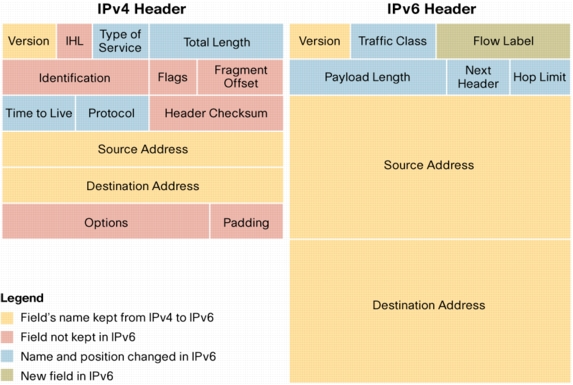
\includegraphics[width=0.75\textwidth]{CiscoHeader}
  \caption {hentet fra Cisco sin nettsider.}
\end{figure}

IPv6 har en annen fordel i ved muligheten for selv-adressering enten via IPv6 Stateless Address AutoConfiguration (SLAAC) som også kan kombineres med DHCPv6 som vil være hva en kaller stateless DHCPv6. I et miljø med potensielt tusenvis av adresserte enheter er dette kritisk. Klienter vil da motta et nettverk prefix på /64 bit via RA (router advertisement) på det lokale nettverket. De resterende 64 bit er hvor SLAAC kommer inn bilde og generer resten av IPv6 adressen ved hjelp mac adressen og EUI-64 metoden (https://tools.ietf.org/html/rfc7043). I tillegg til adressering kan DHCPv6 brukes til distribuere annen viktig informasjon som DNS server til klienter. Vi vil senere se nærmere på dette i praksis. 

Sikkerhet er en viktig del av IPv6 og for å ivareta dette har en IPsec som er ett åpent standardisert rammeverk utviklet av IETF (https://tools.ietf.org/html/rfc2401). Dette gjøres ved hjelpe av kryptering (ESP extension header)  og autentisering på IP laget (AH authentication header). For IPv4 er det pr i dag så og si alltid støtte for IPsec men med IPv6 er dette et fast innebygd komponent. Det vil si at en til forskjell fra IPv4 er garantert å ha denne muligheten. 

Kilder:
%https://www.ietf.org/rfc/rfc2460.txt Introduksjon til IPv6. header
%https://tools.ietf.org/html/rfc6180# transisjon fra ipv4 til ipv6. Nat osv
%https://tools.ietf.org/html/rfc5156 Reserverte IPv6 adresser
%https://tools.ietf.org/html/rfc7043 EUI-64
%https://iot6.eu/ipv6_for_iot EUs forskningsgruppe for IoT6. Litt utdatert.
%https://www.ipv6.com Litt av alt
%https://tools.ietf.org/html/rfc4944

\subsection{6LoWPAN}
I en oppgave som omhandler IoT er det også naturlig å nevne IPv6 sin lillebror, 6LoWPAN. 6LoWPAN er en strømbesparende kommunikasjonsprotokoll som tar i bruk IPv6 på et WPAN. Protokollen er konstruert rundt et krav om lavt strømforbruk da dens bruksområde er små enheter. Dette gjør protokollen til et effektivt verktøy i Tingenes Internett. 6LoWPAN oppnår den lave båndbredden ved å komprimere pakke headeren og en mekanisme for innkapsling. Dette muliggjør bruk av IPv6 pakker over IEEE 802.15.4 baserte nettverk.

\subsection{SigFox og andre aktuelle teknologier}
Sigfox er en LPWAN teknologi designet spesifikt for Internet of Things. Noder koblet sammen gjennom Sigfox bruker lite strøm og kan sende signal over store avstander. Sigfox nettverket består av tre elementer:
\\
\begin{itemize}
	\item Objekter (enheter)
	\item Basestasjoner (gateways)
	\item Cloud (Internett)
\end{itemize}
Sigfox bruker Phase Shift Keying (DPSK) for device-to-cloud kommunikasjon - eller “uplink” - og Frequency Shift Keying (FSK) for Cloud-to-device kommunikasjon - eller “downlink”. Grunnen til at DPSK blir brukt i denne implementasjonen er på grunn av alle forstyrrelsene et signal vil møte på fra den sender signalet, til den treffer gatewayen. Så den passer på at signalet som kommer ut av noden, blir forstått som det samme signalet av gatewayen.
FSK og DPSK og lignende teknologier er viktig for standarder som skal sende signaler over lange distanser med mye støy.

Sigfox har en rekkevidde på rundt 1 km, så den har ikke like god rekkevidde som LoRaWAN, den er heller ikke like utbredt og brukt av forskjellige industrier. Med tanke på dette, og stavanger Smartby så mente vi at LoRaWAN var det bedre valget for en kommunikasjonsstandard med høy rekkevidde, og lav strømbruk.


\subsection{Programmerings språk og verktøy}

\subsubsection{Python}
Python er et tolket objektorientert programmeringsspråk, at språket er tolket vil si at kode tolkes og oversettes til maskinkode under kjøring av programmer\cite{grunnleggendepython} . At språket er objektorientert refererer til at språket benytter seg av objekter ikke prosedyrer. Og objektorientert programmering fører med et fokus på bygge programmer og systemer som er uavhengige av plattform, nettverk og programmeringsspråk, dette gjøres ved å lage objekter som kommuniserer med hverandre. Når objekter først er lagd vil de kunne gjenbrukes, noe som er nyttig om man ikke ønsker å skrive samme kode flere ganger. Selv om Python er objektorientert, trenger det ikke å være det, man kan også skrive prosedyre drevne programmer. Dette gir en større grad av fleksibilitet enn andre programmeringsspråk, selv om Python ofte kan bli sett på som en minimalistisk og streng versjon av Pearl. Da Python er et både populært og velutviklet programmeringsspråk kjører det fortsatt relativt raskt om brukt riktig. Pythons bruksområder er varierte, man kan si at det er et allsidig programmeringsspråk, som kan brukes til alt fra små script til større programmer. Ved UiS blir det undervist som en del av pensum i Webprogrammering og som en del av Websearch og Datamining. 
%https://programmering.wiki.ifi.uio.no/Grunnleggende_Python
%https://docs.python.org/3/tutorial/index.html

\begin{table}[!ht]
	\begin{center}
		\begin{tabular}{ |l|l|l| }
			\hline
			\multicolumn{2}{ |c| }{{\large Python Bruksommråder}} \\
			\hline
			\multirow{1}{*}{\textbf{Felt}} 
				& \textbf{Rammeverk}\\ \hline
			\multirow{6}{*}{Web Programmering}
				& Django\\ 
				& Pyramid\\
				& Bottle\\
				& Tornado\\
				& Flask\\
				& web2py\\ \hline
			\multirow{6}{*}{GUI Utvikling} 
				& tkInter \\
				& PyGObject\\
				& PyQt \\
				& PySide\\ 
				& Kivy\\
				& wxPython\\ \hline
			\multirow{3}{*}{Behandling av tall} 
				& SciPy\\
				& Pandas\\
				& IPython\\ \hline
			\multirow{3}{*}{Programmvareutvikling} 
				& Buildbot\\
				& Trac\\ 
				& Roundup\\ \hline
 			\multirow{3}{*}{System Administrasjon} 
 				& Ansible \\
 				& Salt\\ 
 				& OpenStack\\ \hline
		\end{tabular}
		\caption{Oversikt over bruksommråder for Pythons rammeverk \cite{pythonrammeverk}}
		\label{table:1}
	\end{center}
\end{table}



Pythons syntax er basert på mellomrom, og kan kalles minimalistisk, enkel og klar. Årsaken til dette er fokuset på mellomrom og innrykk, ikke bruk av spesialtegn som ofte blir brukt i programmering. Koden kjøres ved at man oppretter et Python script, for så at Python tolker det linje for linje, og utfører kommandoene som blir kalt i scriptet. I Listing 1, ser vi et eksempel på Python syntax. Programmet henter inn biblioteker, bruker objekter, while løkke og definerer variabler for å skrive temperatur data til ei tekstfil ved et gitt intervall.

\begin{lstlisting}[language=Python, caption=Python eksempel]

from sense_hat import SenseHat
from time import asctime
from time import sleep

sense = SenseHat()

temp = round(sense.get_temperature())
humidity = round(sense.get_humidity())
pressure = round(sense.get_pressure())
message = 'Temperature is %d C Humidity is %d percent Pressure is %d mbars' %(temp,humidity,pressure)

sense.show_message(message, scroll_speed=(0.08),text_colour=[200,0,200], back_colour= [0,0,200])
sense.clear()

while True:
    log = open("weather.txt", "a")
    now = str(asctime())
    log.write(now + " " + message + "\n")
    print(message)
    log.close()
    sleep(30)
    
log.close()
\end{lstlisting}

For programmering innen IoT og programmering på Raspberry Pi, er Python et av de vanligste språkene. Både Python 2 og Python 3 kommer som en del av Raspian Stretch operativsystemet, og språket er så hyppig brukt blant RPi brukere at Raspberry Pi sine egen nettsider har egen dokumentasjon for språket. Det er også lagd egne biblioteker for Raspberry Pi Sense Hat, som har vært en viktig del av testfasen for vårt IoT laboratorium. %https://www.raspberrypi.org/documentation/usage/python/

\subsubsection{Java}
For programmering mot xBee kortene har det vært et alternativ å benytte Java som programmeringsspråk. Java er et objektorientert programmeringsspråk som blir levert med et stort bibliotek, og er et av de mest populære programmeringsspråkene som er utviklet. Det er ofte det første programmeringsspråket studenter læres da det har streng syntaks. I motsetning til Python som baseres på mellomrom, baserer Java seg på spesialtegn. Av denne grunn vises det mer nøyaktig hvor og hva hvilke deler av programmet som kjører, dette kan være både en fordel og en ulempe for nye programmerere. 

Java har et stort utviklermiljø både internasjonal og i Norge, det støtter også de fleste operativsystemer. Av denne grunn er det et veldig relevant språk med tanke på IoT. Språket medfølger også som en del av Raspian Stretch, som har vært en sentral del av IoT laboratoriumet vår. Under testing av xBee sensorer utførte vi flere tester for innlesing av sensor data, men flere av bibliotekene lagt for kommunikasjon med xBee enhetene og ZigBee protokollen er utdaterte. Java har derfor blitt valgt bort til fordel for bruk av Node-RED og Python for programmering. 

\begin{lstlisting}[language=Java, caption=Java eksempel]
    private static class DataReceiveListener implements IDataReceiveListener {
        @Override
        public void dataReceived(XBeeMessage xbeeMessage) {
            System.out.println("------------------------------------------------------------------");
            System.out.println("> " + xbeeMessage.getDevice().getNodeID() +
                    (xbeeMessage.isBroadcast() ? " (broadcast)" : "") +
                    ": " + new String(xbeeMessage.getData()));
            System.out.println("------------------------------------------------------------------");
        }
    }
 \end{lstlisting} 

\subsubsection{Node-RED}
Node-RED er et visuellt programmeringsverktøy utviklet av IBM med IoT som hovedbruksommråde. Node-RED er basert på JSON, og det er mulighet for å implementere funksjoner både i JavaScript og Python. Programmeringsverktøyet baserer seg på å sette inn noder med en gitt funksjon for så å koble sammen noder til de danner et fullkomment program. Plattformen er open source, og har et stort nettbasert sammfun som utvikler egne noder, og utvider plattformen. Node-RED 

\begin{figure}[!ht]
  \centering
      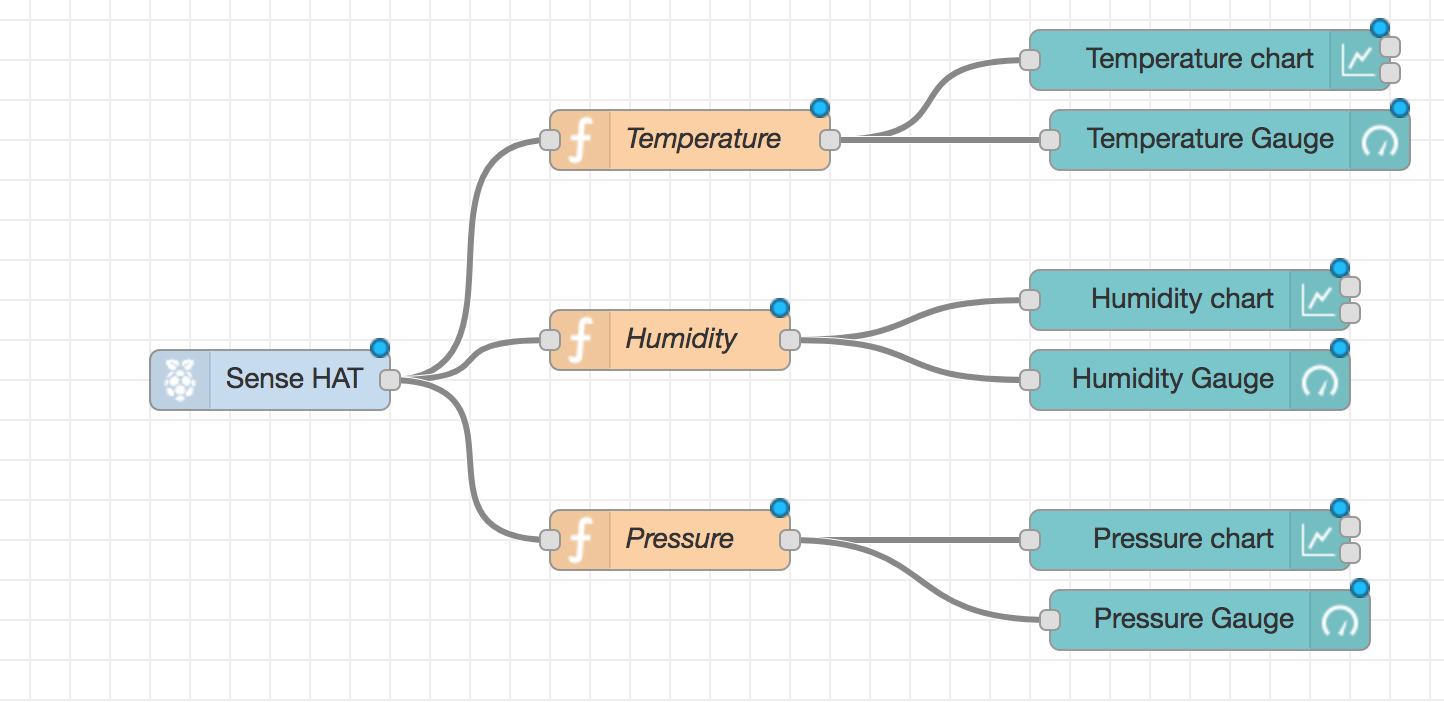
\includegraphics[width=0.6\textwidth]{NodeRedSenseFlow1}
  \caption {Node-RED innhenting av data fra RPi SenseHat og sending til Node-RED Dashboard}
\end{figure}

Fra Figur en har vi et eksempel på hvordan man bruker Node-RED til visuell programmering. Programmeringen er gjort på et web grensesnitt, med noder og relativt lite tradisjonell programmering. For å hente ut web grensesnittet må man besøke ip-adressen til enheten Node-RED kjører på, fulgt av port nummer. I dette tilfellet er det en RPi på det lukkede IoT nettverket på laboratoriumet, med addresse 192.168.1.35 med port 1880.

 \begin{table}[!ht]
	\begin{center}
		\begin{tabular}{ |l|l|l| }
			\hline
			\multicolumn{2}{ |c| }{\large Node-RED Web grensesnitt addressering}\\
			\hline
			\multirow{1}{*}{Fra lokal maskin}
				& http://localhost:1880 \\ \hline
			\multirow{1}{*}{Fra maskin på samme nettverk}
				& http://Node-RED-machine-ip-address:1880 \\ \hline
			\multirow{1}{*}{Node-RED Dashboard} 
				& http://Node-RED-machine-ip-address:1880/ui \\ \hline
		\end{tabular}
		\caption{Oversikt over ip-addresser for å nå Node-RED}
		\label{table:2}
	\end{center}
\end{table}


\begin{figure}[!ht]
  \centering
      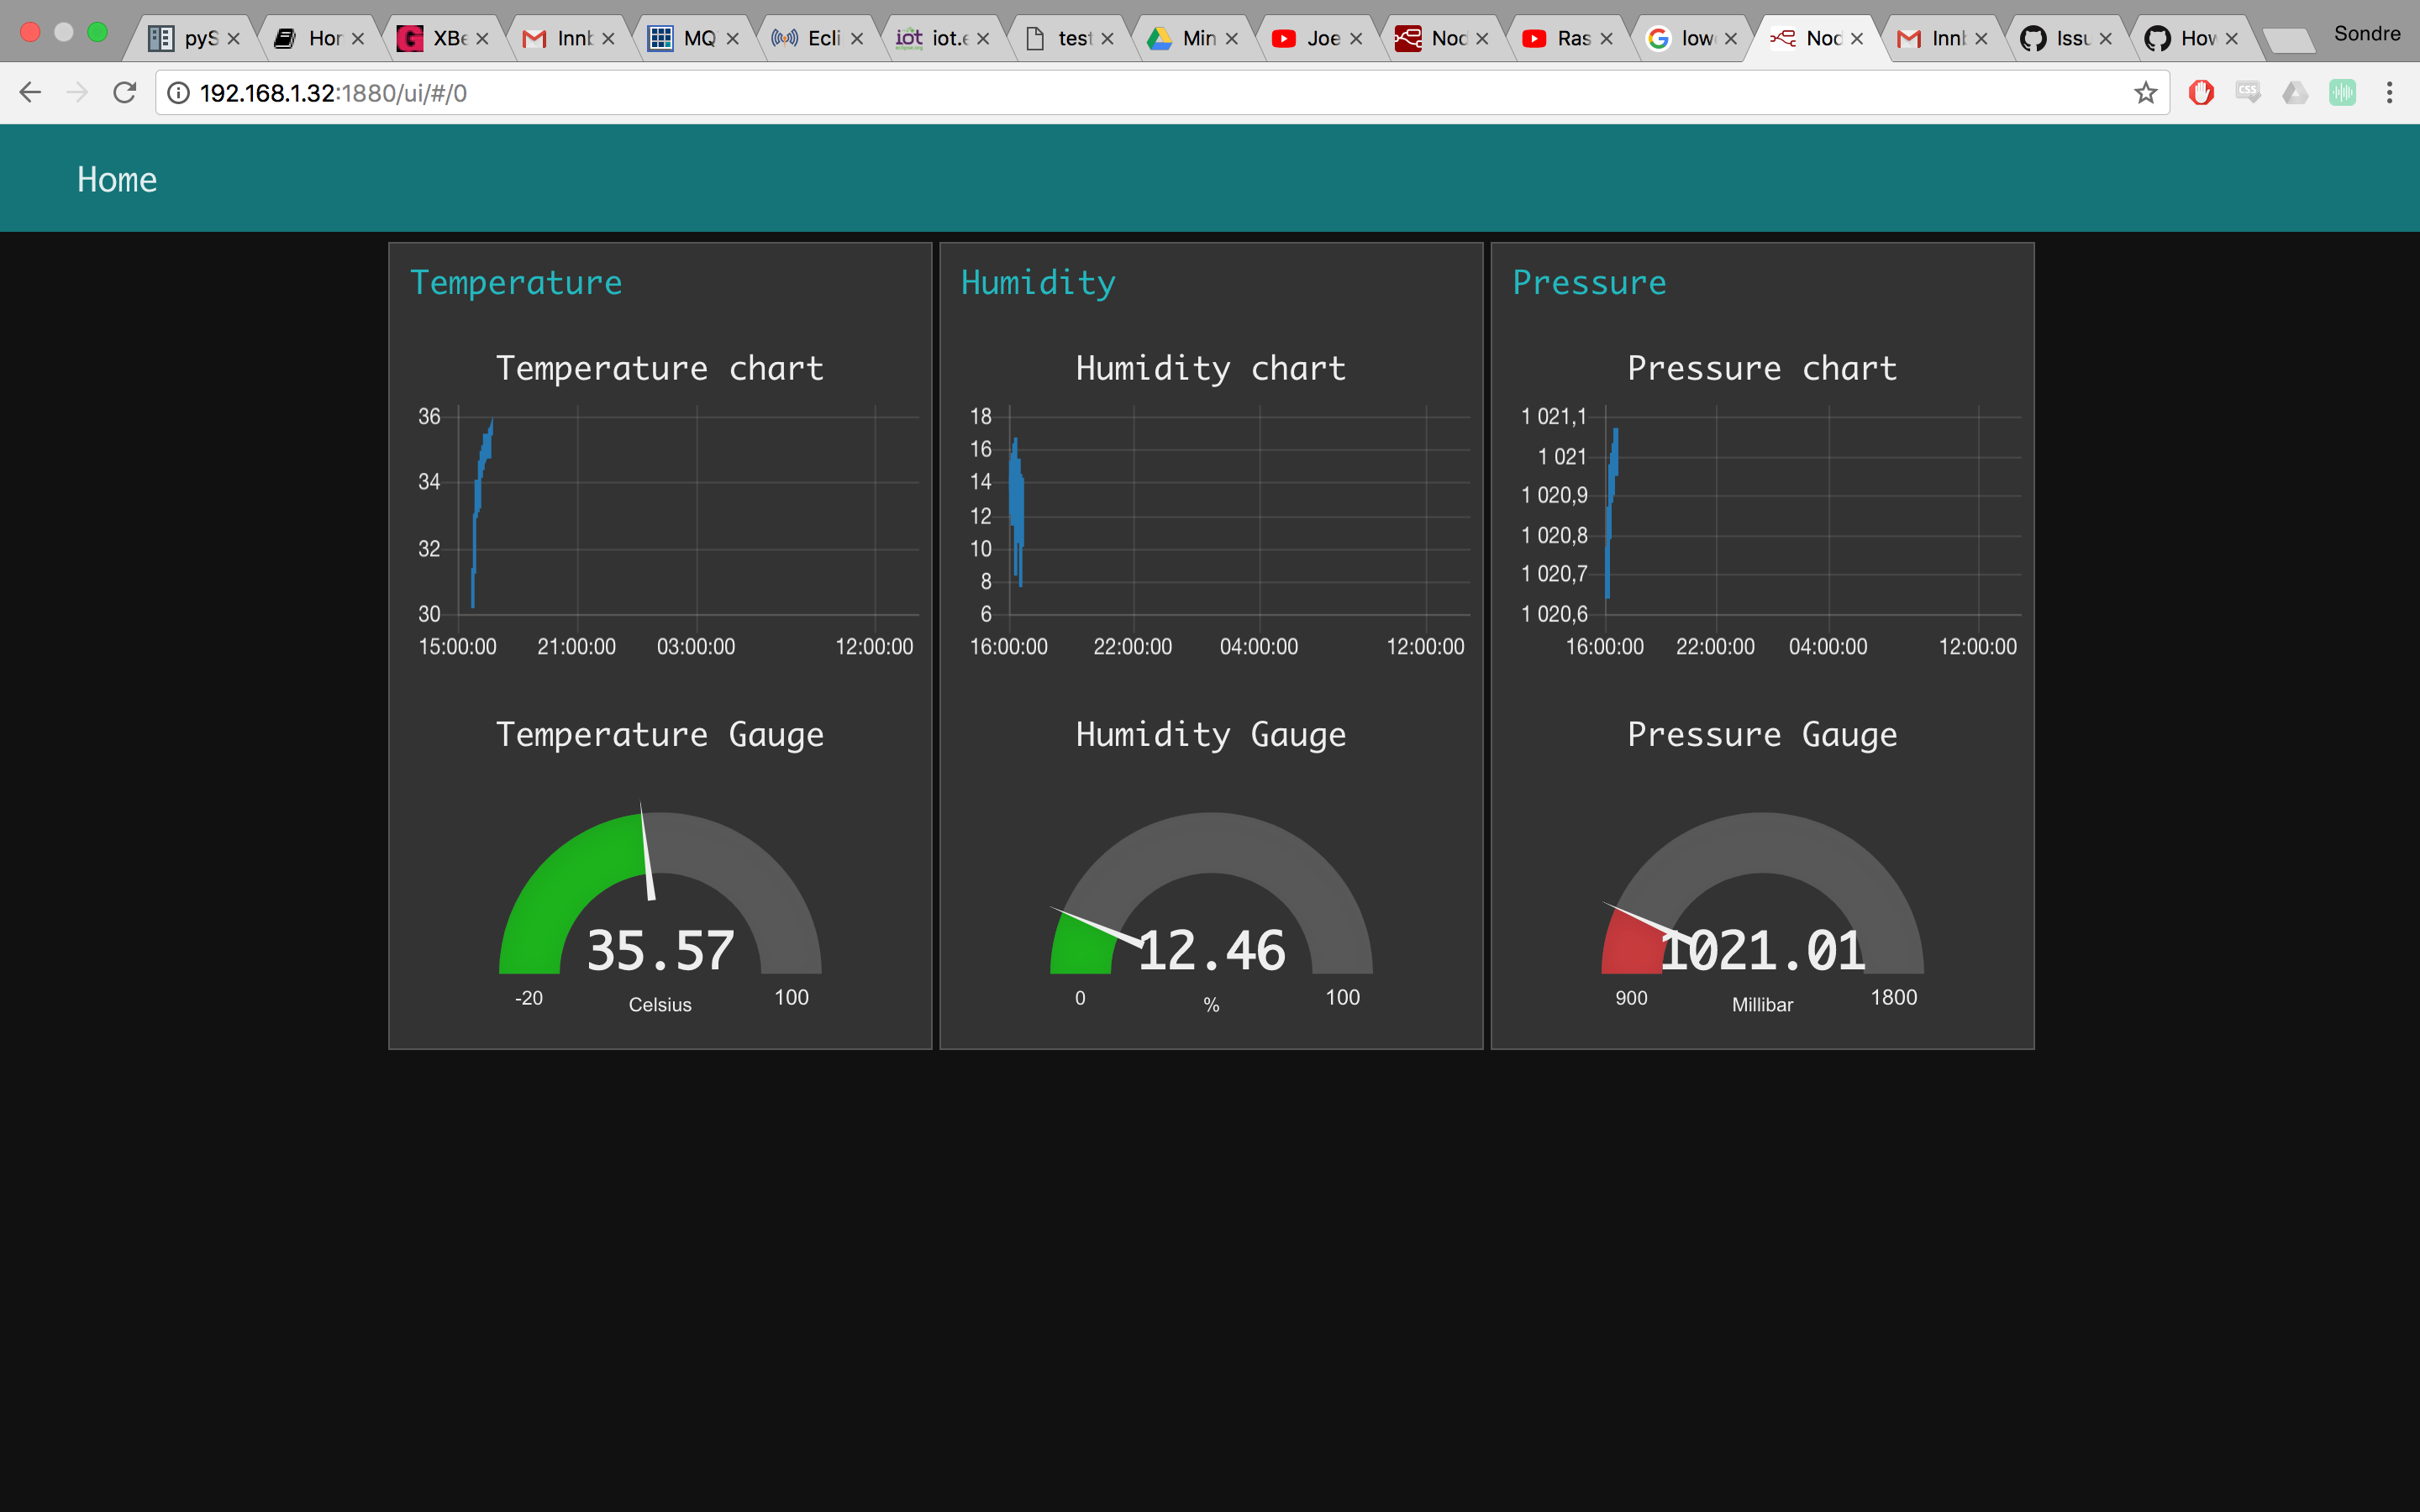
\includegraphics[width=0.9\textwidth]{NodeRedDashboard1}
  \caption {Node-RED Dashboard som viser innhentet data fra RPi SenseHat}
\end{figure}




\subsection{OpenCV}


OpenCV (Open Source Computer Vision Library) er et bibliotek av funksjoner som er laget for bildebehandling og maskinlæring. Det ble offisielt lansert i 1999 av Intel Research for å avansere CPU-intensive applikasjoner, som bildebehandling, og real-time tracking av bevegelse. 

OpenCV er skrevet i C++, men det er bindinger i Python, Java og MATLAB. I vårt prosjekt så har vi kompilert OpenCV med Python bindinger for å kunne kjøre Python scripts for å behandle video-feeden fra RPi kameraet.


\begin{figure}[!ht]
  \centering
      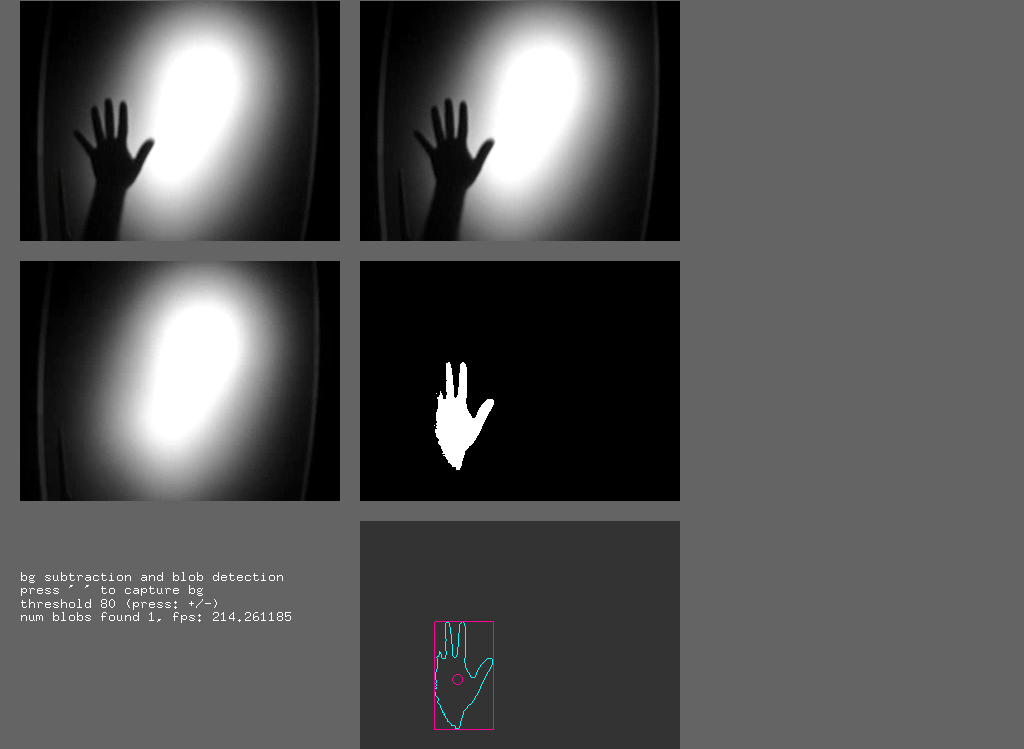
\includegraphics[width=0.65\textwidth]{OfxOpenCV}
  \caption {OpenCV identifisering av bevegelse}
\end{figure}

%----------------------------------------------------------------------------------------
%   PERSONVERN SEKSJON
%----------------------------------------------------------------------------------------


\newpage
\section{Personvern}
I dette avsnittet skal vi ta for oss hensyn til personvern og sikkerhet man må ta høyde for i et IoT laboratorie miljø. Ettersom mye er sensorteknikk og behandling av data er det viktig å ha klart hva UiS sitt ansvar er med tanke på personopplysninger som kan fremkomme under laboratorieoppgaver og daglig drift. Spesielt aktuelt er det nå da EU nye forodning for personvern, heretter referert til som GDPR (General Data Protection Regulation), bli gjeldende fra 25 Mai. Det må nevnes at GDPR ofte har blitt omtalt som direktiv fra EU, mens det i realiteten er todelt med en forordning og et direktiv del hvor sistnevnte omhandler myndighetenes behandling av personopplysninger i straffesaker og er således ikke aktuell her. Det viktig å tydeliggjør forskjellen da en forordning er et krav fra EØS og Schengen avtalen at lovteksten i sin originale form er gjeldende norsk lov. Det er nettopp av denne grunn samt at det for det meste er en innstramming av dagens lovverk, at vi videre vi fokusere på GDPR når det kommer til personvern generelt.

Kilder:
Datatilsynets nettsider, originale lovteksten og Datatilsynets uoffisielle oversettelse
https://www.datatilsynet.no/regelverk-og-skjema/nye-personvernregler/
https://www.datatilsynet.no/globalassets/global/regelverk-skjema/forordningen/uoffisiell-norsk-oversettelse-av-personvernforordningen.pdf
http://eur-lex.europa.eu/legal-content/EN/TXT/PDF/?uri=OJ:L:2016:119:FULL

\subsection{General Data Protection Regulation}
Videre vil en nå se mer på GDPR generelt, men da kun de områder som vil berøre UiS kommunikasjonsteknologi laboratorium og gi anbefalinger for retningslinjer spesifikt for IoT laboratoriemiljøet. Forordningen er gjeldende i Norge fra 25. Mai og UiS vil etter dette vurderes etter den nye lovteksten. GDPR omhandler lagring og behandling av personopplysninger og treffer både dataeier/ databehandlingsansvarlig og databehandler. I de fleste scenarioer vil Universitet i Stavanger innehave begge roller men det er noen viktige distinksjoner mellom databehandler og databehandlingsansvarlig som må nevnes. Sistnevnte vil være den som iverksetter databehandling og således må ha fastsatt formålet og metoder. Det er også den som i størst grad er rettslig ansvarlig. Databehandler har også et ansvar men det kommer mer på den faktiske behandlingen av data. Ved transaksjon av data mellom partene skal det foreligge databehandleravtale som tar for seg databehandlers ansvar.  
 
Informasjon klassifiseres som personopplysninger dersom den i seg selv eller i samsvar med annen informasjon, kan identifisere en person direkte eller indirekte. 

Behandling av personopplysninger er definert som alle operasjoner som utføres med/på personopplysninger, manuelt eller automatisert. Det innebærer altså alt en gjør med dataene, inkludert anskaffelse og sletting. 

Alle berørte av datainnsamling som kan kategoriseres som personopplysning skal frivillig gis samtykke til at dette er greit. En må sørge for at samtykker er godt informert og samtykket skal være klart og tydelig.

\paragraph{Viktige endringer og tillegg fra dagens lovverk som her er aktuelle.}
\begin{itemize}
	\item Større økonomiske konsekvenser ved brudd med bøter på opptil 4 for databehandlingsansvarlig og opptil 2 for databehandler.
	\item Det stilles nye krav til dokumentasjon, altså hvordan og hva av informasjon som blir lagret og behandlet. Hvor de kommer fra og blir lagret
	\item Det skal være åpenhet på hva som blir lagret og hvorfor. Dette skal ha et klart og tydelig språk
	\item Biometriske data regnes nå som sensitiv personopplysninger
	\item Overføring av data som regnes som personopplysninger til land utenfor EØS er ikke lov, dog finnes flere unntak
	\item Flere og utvidede rettigheter for EU/EØS borgere
	\item Krav om personvernombud i organisasjoner med databehandler og databehandleransvarlig roller
	\item Strenger krav til avviksrapportering.
	\item Krav til innebygd personvern, altså at det personvernet settes i første rekke i nye prosjekter, løsninger, tjenester ol. Dette er hva som kalles personvern som standardinnstilling.
\end{itemize}

\subsection{Retningslinjer spesifikt for IoT lab}
Som tidligere nevnt er det i Internet of Things natur mye innsamling og behandling av data og det er derfor viktig å foreta flere vurderinger i forkant av øvelser og prosjekter. Det er databehandleransvarlig sin oppgave og ansvar å kartlegge risiko og konsekvenser før behandling.

\begin{itemize}
	\item Vil det samles inn data som kan klassifiseres som personopplysninger og i så fall er dette er dette nødvendig for prosjektet. Er det mulig å anonymisere informasjonen.
	\item Sørge for åpenhet og samtykke fra personer som kan bli berørt
	\item Påse at uvedkommende ikke får tilgang til informasjon
	\item Dersom informasjon blir lagret må en kunne påse at informasjon blir slettet igjen når det ikke lenger har formål eller ved ønske fra berørte. 
\end{itemize}

Informasjon som innhentes i IoT laboratoriumet vil hovedsakelig være sensordata Så det er hva vi vil fokusere på videre. Sensordata som innhentes og som kan klassifiseres som personopplysninger kan være biometriske data som stemme eller fingeravtrykk. Det vil også være bilde og video hvor person er identifiserbar. En må også huske at dersom f.eks bilde fra et kamera eller data fra en bevegelsessensor i seg i selv ikke kan identifisere en person, så faller det også under personopplysning dersom det i samsvar med annen info kan identifisere personen. Står bevegelsessensor i rom med meget begrenset adgang kan det brukes til kartlegge en spesifikk person sine bevegelser. Miljødata som temperatur, luftfuktighet kan også indikere bevegelse av personer i samsvar med andre datasett. En må derfor være obs på både hva og hvor en samler sammen informasjon. Dette er spesielt viktig dersom det vil være lett tilgjengelig på eksempelvis internett eller skjerm. \newline
I noen tilfeller vil en kunne bruke  ekstern databehandler av innsamlet informasjon. Det kan være en plattform som www.thethingsnetwork.org, lagring i skyen og/eller en annen form for tjeneste. Dersom dette er betegnet som personinformasjon er det flere ting en må ta hensyn til.

\begin{itemize}
	\item Plattform, nettside eller tjeneste bør være innad i EU/EØS
	\item En må ha en databehandleravtale
	\item Vi må kunne påse at sletting av data er mulig hos ekstern databehandler. Det er databehandlingsansvarlig sitt ansvar at informasjon blir slettet, selv på internett
\end{itemize}

Ved sikkerhetsbrudd som kan medføre tap av personopplysninger må UiS personvernombud umiddelbart varsles. Det er krav at Datatilsynet skal varsles så snart som mulig om hendelse og senest 72 timer etter dette er oppstått. 

Vi har i denne oppgaven fokusert på unngå behandling av informasjon som kan klassifiseres som personopplysning. Alle data som samles inn i daglig drift eller i oppgave kan sies å være anonym informasjon. Dette er hovedsakelig for å følge av kravet om innebygd personvern i nye prosjekter med personvern som standardinnstilling. Som en bonus gir dette oss mer frihet til hva en gjør med dataene. Da dette er tiltenkt å være en start for en utviklende IoT laboratorium er det likevel viktig å ha på plass rammeverket for hva og hvordan vi behandler sensitiv informasjon. Det kan tenkes det kommer fremtidige prosjekter hvor det ikke er snakk om anonyme data. I de tilfeller anbefales det å ta det med UiS personvernombud i forkant

%----------------------------------------------------------------------------------------
%   VALG AV UTSTYR SEKSJON
%----------------------------------------------------------------------------------------

\newpage
\section{Valg av utstyr}
Under forstudiet for et IoT laboratorium er utvelgelsen av utstyr en sentral del av prosessen, etter undersøking og valg av teknologier laboratoriumet skal støtte må utstyret på plass. Under utvelgelsen er det nødvendig at utstyret skal kunne brukes sammen med utstyr som allerede er tilgjengelig på lab, og at det så langt som mulig benytter samme operativsystemer og syntaks som studenter ved Kommunikasjonsteknolgi er vandt med. Dette er med å påvirke valg av aksesspunkter i stor grad, utstyret tatt i bruk av studenter i Kommunikasjonsteknologi er levert av Cisco det vil da skape forvirring om IoT laboratoriumet implementerte bare Huawei utstyr. Dette er noe flere av gruppens medlemmer har erfart fra arbeid hos Altibox med både Cisco og Huawei utstyr.

\subsection{Eksisterende utstyr}

\subsubsection{Cisco 2901 Integrated Services Router}
Dagens komtek laboratorium har flere routere og switcher fordelt på 7 rack. Vi har fått tildelt 1 router og 1 switch til bruk i denne oppgaven. Disse er plassert i rack ved navn “Antarktisk”. 

Vi kan starte med routeren, en Cisco Catalyst 2901. Ut i fra Cisco sin egen beskrivelse av produktet er dette en router beregnet som en del at større nettverk i hva de kaller “Bordeless Network”\cite{cisco2901} %(https://www.cisco.com/c/en/us/products/routers/2901-integrated-services-router-isr/index.html). 
Det vil si konnektivitet på tvers av lokasjoner, til skyen og et mer åpent og tilgjengelig nettverk som i eksempelvis gjestenett, tilgang for eksterne konsulenter, delvis tilgang til andre plattformer osv. Til tross for at dette er en eldre modell som er end of sales er det interessant å se hvordan nettverk verden over var og er i endring hvor vi ser den naturlige utviklingen videre med IoT\cite{ciscosky} %(https://www.cisco.com/c/dam/en_us/solutions/industries/docs/retail/Retail_BN_AAG.pdf). 
Som router isolere den naturligvis laboratoriemiljøet samt å route trafikk til internett via Universitetets eget interne nettverk, UNIX. I praksis fungerer denne routeren på mange måter som en IoT gateway(https://tools.ietf.org/html/rfc7452) ved at den aggregerer IoT nettverkene videre mot skyen. C2901 er en Dual Stack router som støtter både ipv4 og ipv6 parallelt. Dette er en fordel da vi i denne oppgaven hovedsakelig har jobbet over ipv4 men har lagt til rette for ipv6 for fremtidige prosjekt. Av integrerte porter har vi 2 AUX console og 2 Gigabit Ethernet porter hvor vi bruker sistnevnte til uplink mot UNIX og downlink mot switch. Ellers har den 4 Enhanced High-Speed WAN Interface Cards (ehwic) hvor den en i modul 1 har kort med 2 serial porter. Det var i hovedsak en funksjon routeren mangler som vi savnet, nemlig NAT-PT som er en måte NAT'e mellom IPv6 og IPv4 adresser på samme router. Akkurat dette samt andre IPv4 to Ipv6 alternativer er noe vil vi se nærmere på senere i dette dokumentet. 


\begin{figure}[!ht]
  \centering
      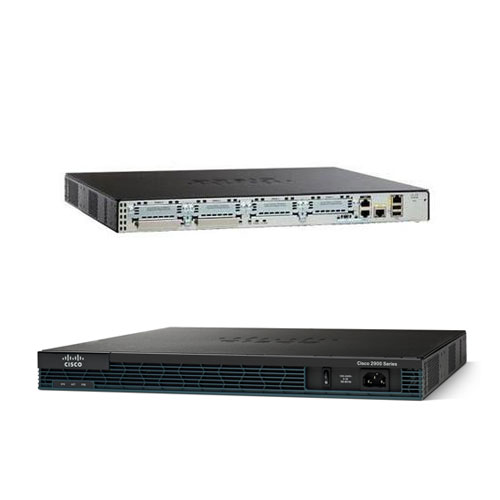
\includegraphics[width=0.5\textwidth]{C2901}
  \caption {C2901 router i Cisco sin Catalyst 2900 serie.}
\end{figure}


\subsubsection{Cisco WS-C2960 switch}
Cisco WS-C2960 er lag 2 switch, den opererer altså kun med mac adresser. Dette er en 2960-24TT-L modell som har 2 Gigabit Ethernet porter hvor den ene benyttes til uplink. Ellers har den 24 Fast Ethernet porter som vi benytter 2 av. Switchen er fixed unit, det er altså ikke mulighet for utvidelse av flere porter. Til laboratoriumets formål skal det likevel være god nok port tetthet. %(https://www.cisco.com/c/en/us/products/collateral/switches/catalyst-2960-series-switches/prod_bulletin0900aecd80322c22.html)

\begin{figure}[!ht]
  \centering
      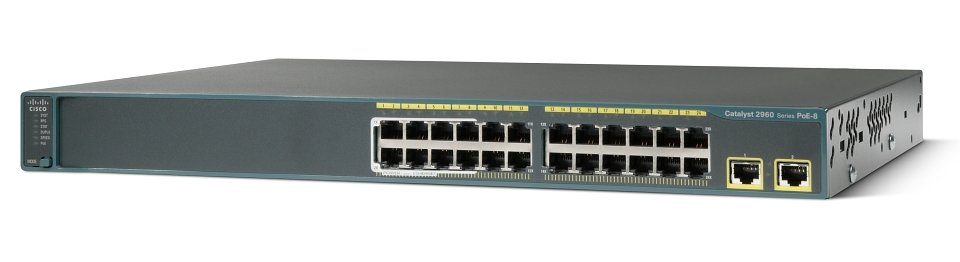
\includegraphics[width=0.5\textwidth]{C2960}
  \caption {Cisco WS-C2960-24TT lag 2 switch}
\end{figure}

\subsection{Aksesspunkt}
Under bygging av et IoT laboratorium er et robust WiFi nettverk dedikert bare til IoT laboratoriumet veldig viktig. WiFi protokollen vil gjøre det mulig å teste bygging av egne MQTT servere, det vil føre til enkel båden sending og mottagning av data gjennom MQTT. WiFi muliggjør utvikling av aplikasjoner for smart telefoner som for eksempel sender MQTT data med en beskjed om så slå av og på en sensor. WiFi er også en stor del av grunnmuren i et IoT laboratorium da det er protokollen som blir tatt i bruk for publisering til Internett. Det vil også være mulig å koble opp mer komplekse enheter, som for eksempel et kamera  til WiFi. Kamera krever både mer strøm og høyere bådbredde en hva som er vanlig for andre IoT protokoller. Kamera kan eksempelvis bli brukt i en personteller eller til å registrere bevegelser.  Egen WiFi for IoT laboratoriumet gjør det også enklere for studenter å jobbe på laboratoriumet da det ikke er sterkt signal fra Eduroam i E-472. Det er med andre ord utrolig viktig å velge et robust aksesspunkt som dekker hele laboratoriumet. I denne delen skal vi se på hvilke aksesspunkter som har blitt vurdert nøye og hvilket som ble valgt.

\subsubsection{Cisco Small Buisness WAP561}
Cisco WAP561\cite{ciscowap} er et aksesspunkt for små bedrifter, som benytter seg av PoE teknologi, støtter aksesslister, IPV6, Spanning Tree Protocol og det meste annet som er nødvendig for en robust infrastruktur. Dette kombinert med lav pris og at utstyret på kommunikasjonsteknologi laboratoriumet allerede er levert av Cisco førte til at dette aksesspunktet ble valgt som beste kandidat for et IoT laboratorium. Cisco WAP561 dekke alle behov for dagens IoT laboratorium og mer. 

\begin{figure}[!ht]
  \centering
      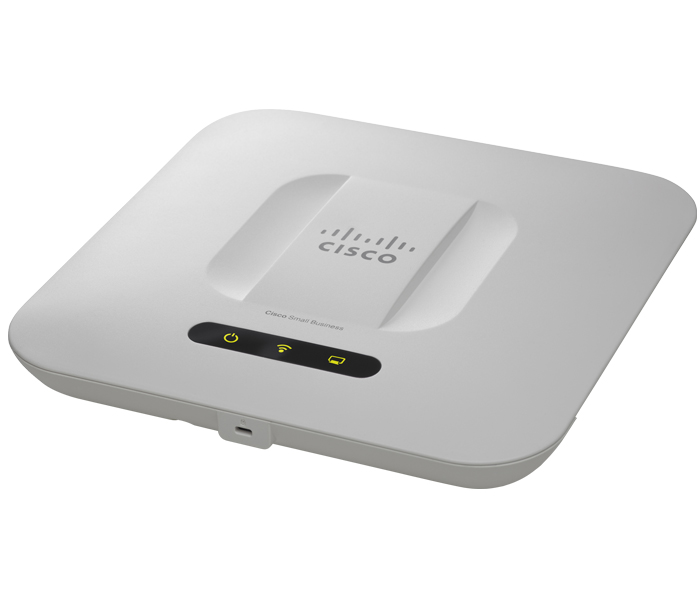
\includegraphics[width=0.5\textwidth]{ciscowap}
  \caption {Cisco Small Business WAP561 aksesspunkt}
\end{figure}


\subsubsection{Cisco Aironet 2702i }
Et alternativ til Cisco WAP561 er Cisco Aironet 2702i\cite{ciscoaironet}, et større og kraftigere aksesspunkt. Cisco Aironet 2702i har både lenger rekkevidd, og mulighet for raskere overføringshastiget. Dette aksesspunktet ble valgt bort da det ikke er behov for verken rekkevidden eller hastigheten på dagens IoT laboratorium.

\begin{figure}[!ht]
  \centering
      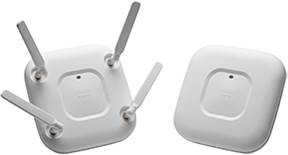
\includegraphics[width=0.5\textwidth]{ciscoaironet}
  \caption {Cisco Aironet 2702i aksesspunkt}
\end{figure}


\subsubsection{Cisco Meraki Serien}
Under utvelgelsen av aksesspunkter ble Ciscos Meraki\cite{ciscomeraki} serie vurdert. Cisco Meraki Serien er aksesspunkter som er designet med IoT i tankene, og støtter flere dataprotokoller en andre aksesspunkter. Meraki serien har støtte for EEE 802.11b, IEEE 802.11a, IEEE 802.11g, IEEE 802.11n, IEEE 802.11ac Wave 2. Ulempen med Meraki serien er at det må brukes Cisco egne Cloud Manager for bruk av aksesspunktene, og dette vil sette restriksjoner på implementering av andre teknologier. Etter ønske fra veileder om så lite bruk av skytjenester som mulig valgte vi derfor å ikke kjøpe inn aksesspunkter fra Meraki serien.

\begin{figure}[!ht]
  \centering
      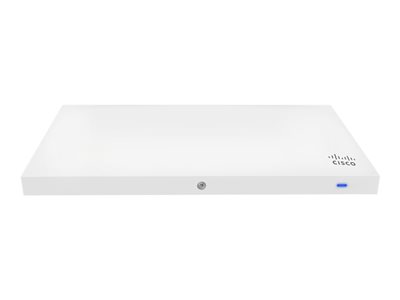
\includegraphics[width=0.5\textwidth]{ciscomeraki}
  \caption {Cisco Meraki MR33 Cloud Managed aksesspunkt}
\end{figure}


\subsection{Raspberry Pi}
En sentral del av vår fremlagte løsning for et IoT laboratorium er mikrodatamaskin Raspberry Pi. Tidligere i rapporten har vi sett på den tekniske siden av RPi, i denne delen vil vi argumentere for hvorfor det har vært et godt valg som en sentral komponent i IoT laboratoriumet vår. Valget av Raspberry Pi ble tatt med hensyn til brukervennlighet, støtte for relevante teknologier, mulighet for utvidelse, pris og til sist et fokus på så lite lodding og kabling som mulig. Sistnevnte punkt er relevant da det ikke vil være krav om kunnskap i konstruering av datamaskiner o.l. for bruk av laboratoriumet. 

\subsubsection{Konkurrenter}

Ved valg av hvilken mikrodatamaskin som skal fungere som hjernen i en IoT lab er det flere alternativer til RPi. En av de sterkeste utfordrerne er Arduino METRO 328, dette er et Arduino kort kombinert med Adafruit sin spesiallagde IoT hat. I likhet med RPi har denne flere GPIO pinner for tilkobling av sensorer, den har også USB til seriell tilkobling, LED lys for testing og sist men ikke minst et stort bibliotek for programmering. Ulempene med Arduino METRO 328 er at den ikke støtter WiFi og at den ikke har HDMI utgang, noe som begrenser dens bruksområde. Det er verdt å nevne at om det skulle være behov for implementering av flere sensorer i det eksisterende nettverket vil denne stille sterkere enn RPi da behovet for HDMI og en ZigBee gateway har blitt dekket av RPi. Arduino UNO er en annen sterk konkurrent, selv om Arduino UNO i seg selv ikke vil kunne måle seg med RPi er det her mange muligheter for utvidelser. Det at man må tilkoble utvidelser og konfigurere allt opp på egenhånd gjør at RPi er et bedre valg da denne labben skal kunne brukes uten forkunnskap i datamaskinarkitektur. Det vil antagelig også kunne by på problemer for studenter om de ønsker å koble opp egne enheter.

\subsubsection{Fordeler med Raspberry Pi}

Med hensyn til brukervennlighet stille RPi sterkt i forhold til sine hovedkonkurrenter, det er flere grunner til dette. Raspberry Pi Model 3B har flere tilkoblingsmuligheter i form av USB/Seriell porter, Ethernet, HDMI, Bluetooth og WiFi. Dette kombinert med den lave prisen gjør det til en vinner innen IoT. Det at RPi har en fire kjernet 64-bit ARM 1.2GHz prosessor og 1 Gb RAM gjør at den er mer en kraftig nok til å være kjernen i et lab nettverk. Det vil så klart kunne være behov for utvidelser dersom nettverket skulle vært industriell størrelse. RPi har også hele 40 GPIO pinner og mulighet for tilkobling av både kamera og touchscreen ved bruk av en designer DSI port. For å finne andre produkter med lignende tilkoblingsmuligheter og lik fleksibilitet er 


\subsection{ZigBee}
I denne delen av rapporten vil vi ta for oss noen av valgene vi har tatt rundt ZigBee opsettet på lab. Vi vil for det meste se på utstyret vi ende opp med å velge, men også presentere andre mulige opsett. 

\subsubsection{Digi International XBee Mesh 2.4GHz ZigBee Development Kit}
For å sette opp ZigBee ble det fort klart at det enkleste valget med tanke på en IoT lab var xBee sendere. Disse kombinert med et spesiallaget kort for utvikling gjør det lett å sette opp et enkelt ZigBee mesh nettverk. Denne pakken vil gjøre det lett for studenter å utforske hvordan ZigBee virker, hvordan mesh nettverk virker, samtidig som denne løsningen var mye rimeligere enn andre alternativer. Vi kom til konklusjonen at ZigBee ikke var den viktigste protokollen å fokusere på, selv om det er en mye brukt protokoll innenfor IoT kom vi fram til at for eksempel LoRaWAN trengte mer fokus. ZigBee leverer også flere ferdige løsninger som også ble vurdert, men for en lab ble disse lite funksjonelle. Grunnen til dette er at man ønsker at studentene skal få sette opp alt fra bunnen av, og de fleste ferdige løsningene ikke gir denne muligheten. Det har vært en viktig del av valget av ZigBee utstyr at så lite skal være konfigurert på forhånd som mulig. Dersom vi hadde valgt en ferdig designet ZigBee gateway og kjøpt inn flere sensorer, ville ikke dette gitt muligheten for innsyn i hvordan IoT virker. De fleste ferdig gatewayer kommer med et ferdig designet interface for tilkobling, som regel både via internett og via mobil applikasjoner. 

Utstyret som følger med våre ZigBee moduler vil gi en enkel lavkostnads måte for studentene å sette opp et fullstendig ZigBee mesh nettverk med en rimelig rekkevidde. Ved optimale forhold vil utstyret klare å sende og motta fra 3200 meter, men det vil så klart bli en del kortere da betongvegger o.l. vil begrense signalstyrken.  En mer realistisk innendørs rekkevidde vil være omtrent 60 meter i følge leverandør. Utstyret vi har valgt sender på den tradisjonelle 2.4GHz frekvensen, og kanalene  15, 20, 25 og 26. Dette vil ikke kollidere med 802.11.n wifi kanalene som sender på 2.4GHz, men på kanal 1, 6 og 11. Med tre av disse modulene vil vi kunne bygge et lite nettverk, og vise at konseptet virker samt hvordan det virker. 
Dersom vi skulle brukt mer penger på ZigBee ville det ha vært lett å utvide for eksempel rekkevidden på labben ved å kjøpe dyrere antenner og moduler av samme selskap. Det hadde også vært en fordel å kjøpe inn flere moduler og hovedkort for å kunne bygge et større nettverk. Vi har valgt å ikke handle inn mer en tre moduler og hovedkort da dette er nok til å demonstrere konseptet.

\begin{figure}[!ht]
  \centering
    \reflectbox{%
      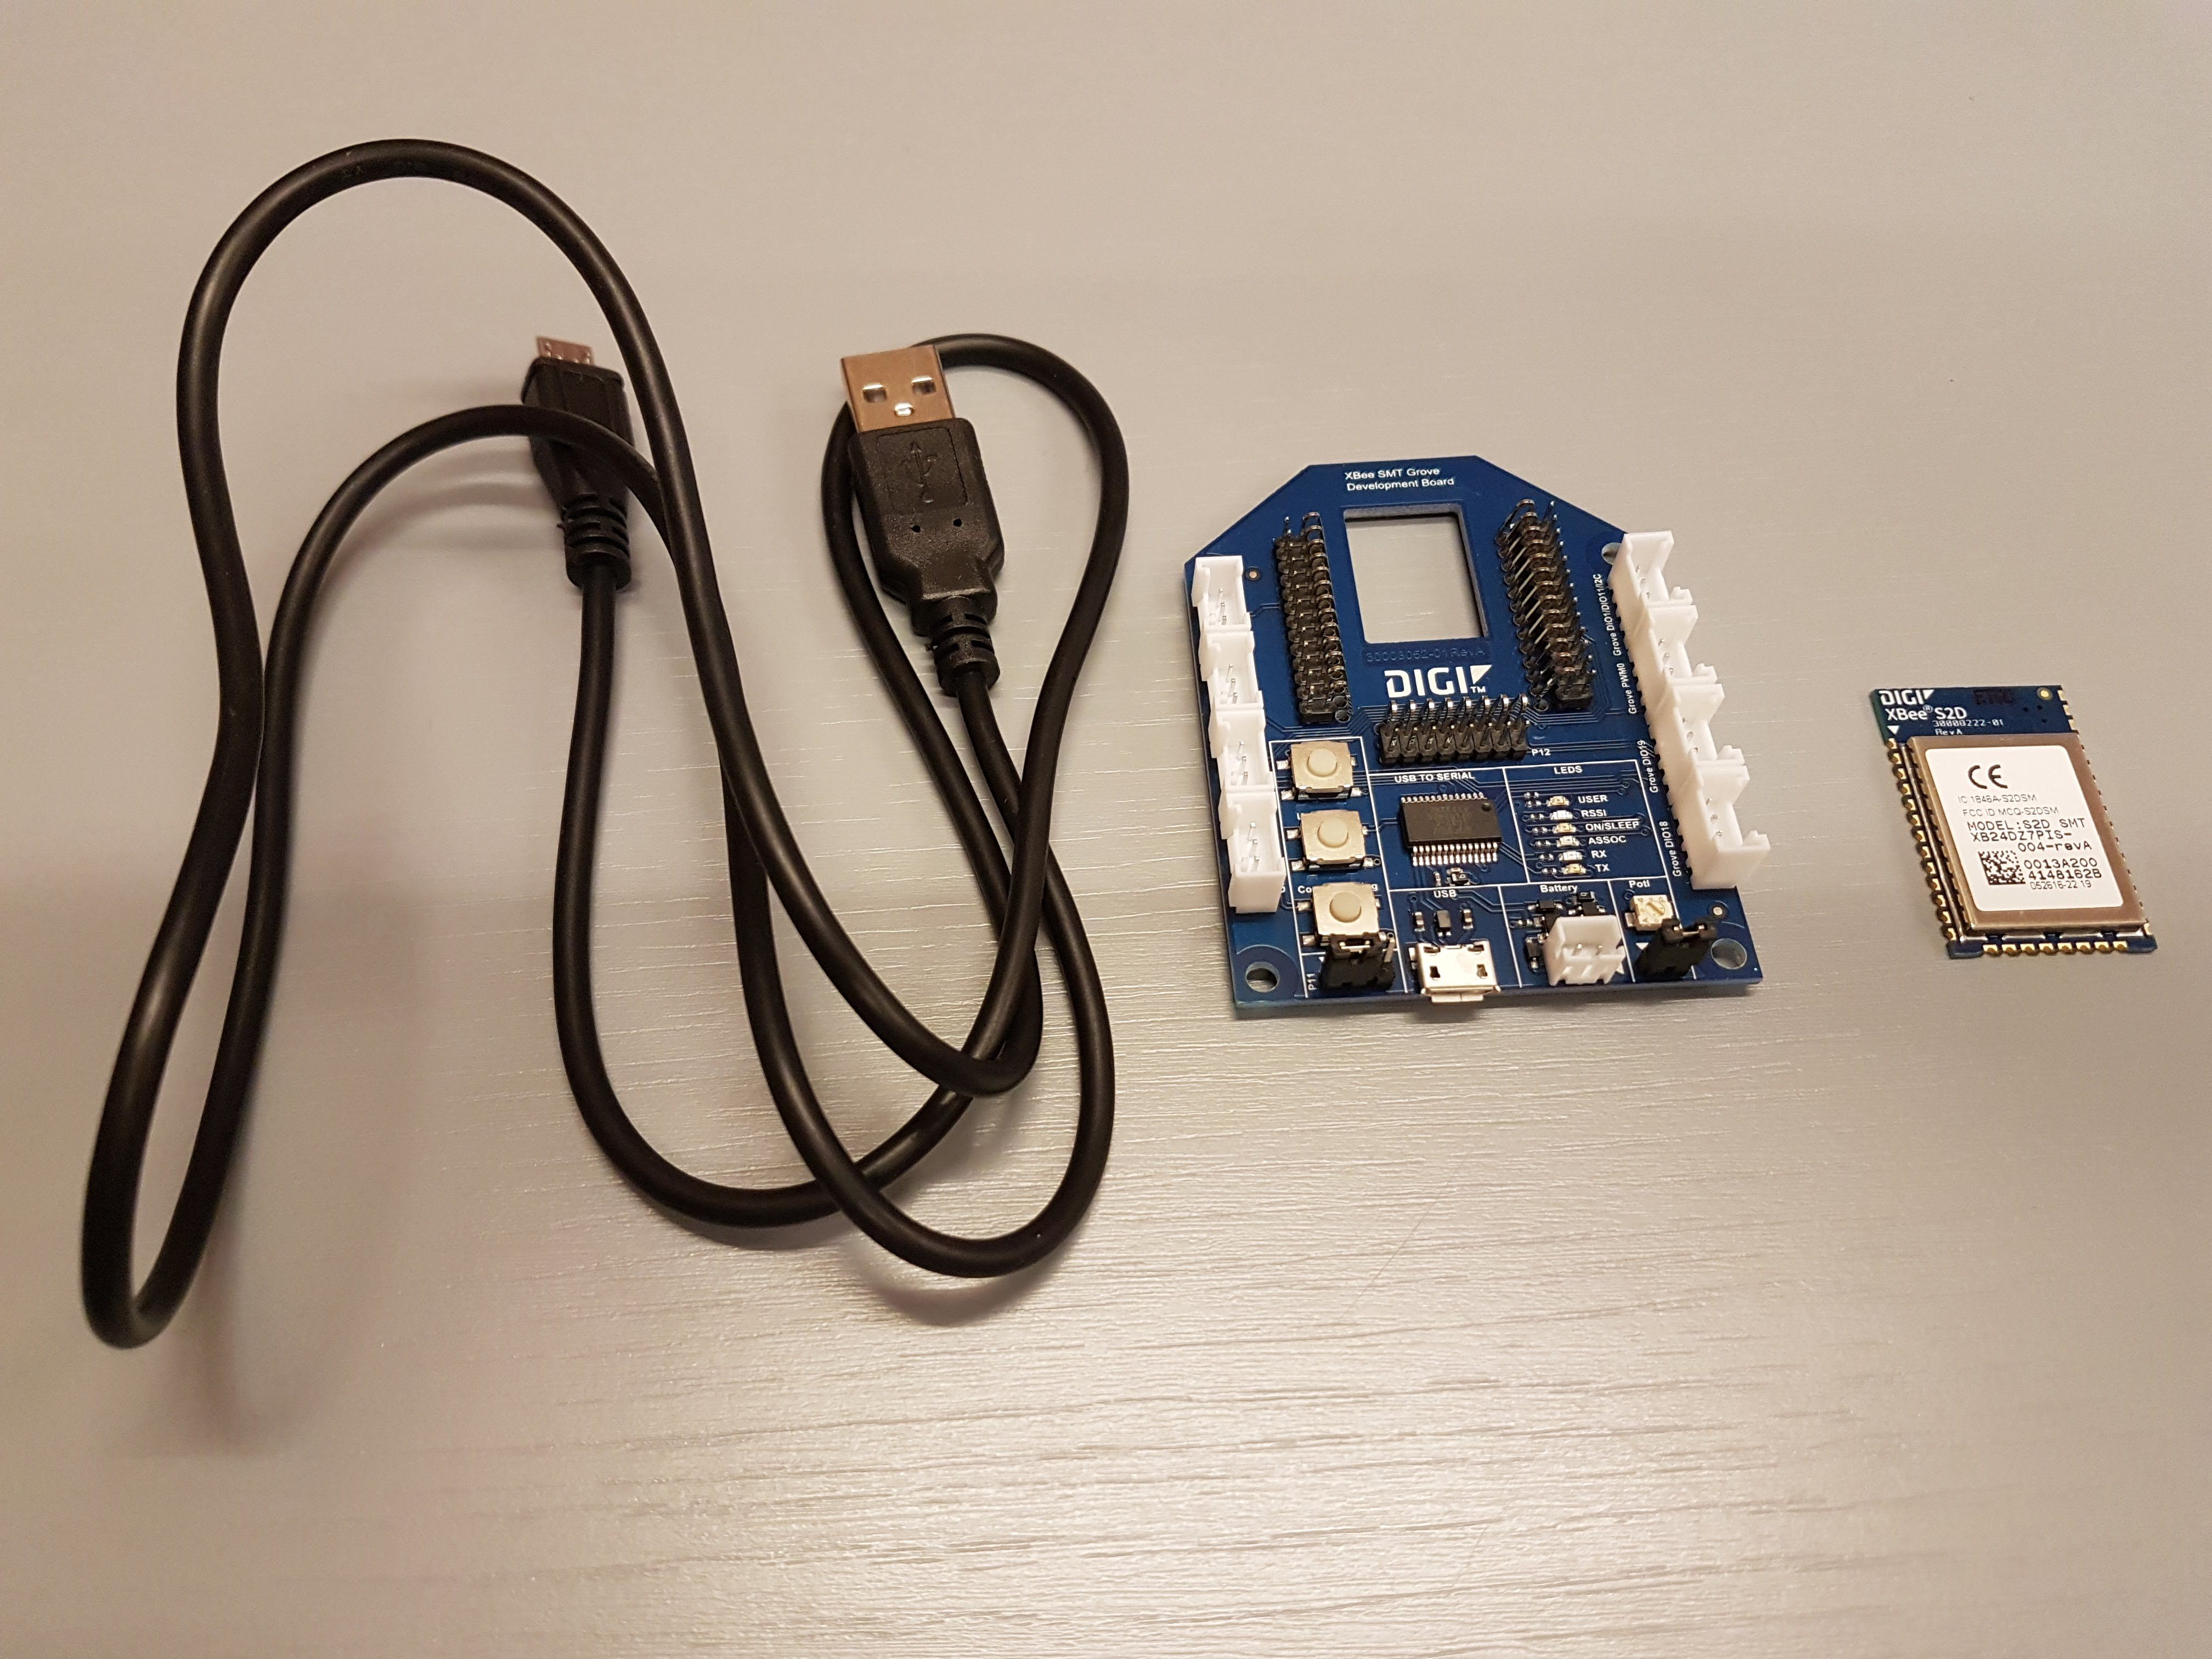
\includegraphics[width=0.8\textwidth]{xBeeHardware}}
  \caption{Avbbilding av et xBee Development Board, S2D senderen og medfølgende mikro USB kabel.}
\end{figure}

Dersom Universitetet i Stavanger ønsker å utvide IoT labben og fokusere mer på ZigBee vil dette være mulig på en enkel og kostnadseffektiv måte. Det eneste som kreves for utvidelse av flere antenner og et hovedkort/utvikler kort. Å utvide labben vil kunne være interessant da det finnes mange forskjellige ZigBee moduler. Dersom man ønsker å lære studenter hvordan forskjellige antenner virker for eksempel, vil dette være lett og rimelig å implementere da xBee modulene støtter flere typer antenner. Da vil studenter kunne se hvordan forskjellige antenner vil påvirke rekkevidden.


\subsection{LoRaWAN}
LoRaWAN er en teknologi som er mye brukt innen IoT, LoRaWAN er spesiellt mye brukt i Stavanger-regionen. Teknologien er designet for sending av data som krever lav båndbredde. LoRaWAN sender på forskjellige frekvenser avhengig av hvor man befinner seg i verde, men uansett hvor man befinner seg i verden, sender det på lengre bølgelengder enn de andre protokollene i IoT labben. LoRaWAN sender faktisk saktere enn morsekode, dette begrenser bruksommrådet på en lab. Vi har derfor valgt å sette fokus på muliggjøring av sensor testing i mindre skala.  


\subsubsection{Cisco Wireless Gateway for LoRaWAN}
Cisco Wireless Gateway\cite{ciscolora} for LoRaWAN er en robust trådløs LoRaWAN Gateway, denne støtter bølgelengder for alle geolokasjoner. Cisco Wireless Gateway for LoRaWAN er en industriell gateway lagd for utendørs plassering. Den er lagd for utendørs plassering fordi den avgir elektromagnetisk strålig som er så pass kraftig at den ikke bør plasseres innendørs. Innendørs plassering vil begrense rekkevidden, og det vil ikke være optimalt å plassere denne på lab. Denne gatewayen ble ikke tatt i bruk da det ikke er behov for industriell skala LoRaWAN implementering. 

\begin{figure}[!ht]
  \centering
    \reflectbox{%
      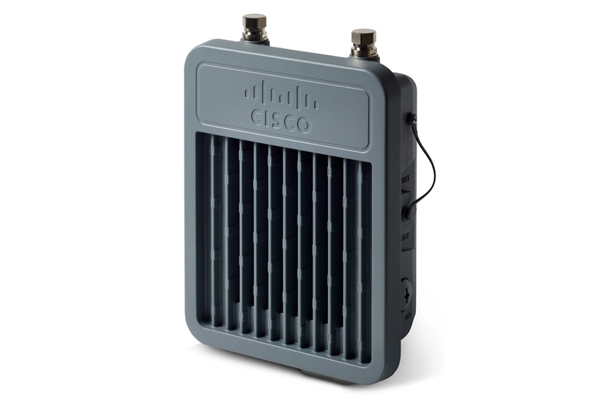
\includegraphics[width=0.7\textwidth]{ciscolora}}
  \caption{Cisco Wireless Gateway for LoRaWAN}
\end{figure}


\subsubsection{Kerlink Wirnet iFemtoCell}
Kerlink Wirnet iFemtoCell er en LoRaWAN gateway designet for forlengelse av LoRaWAN bølger innendørs. Denne gatewayen er betydelig mindre, og betydelig mindre kostbar enn Cisco Wireless Gateway for LoRaWAN. Kerlink Wirnet iFemtoCell har mulighet for sending over 9 forskjellige kanaler, og er kompatibel med Wanesy Small Private Network løsningen for bygging av et eget LoRaWAN nettverk. Kerlink Wirnet iFemtoCell kan derfor brukes som LoRaWAN sender og mottaker i et lab miljø. Rekkevidden er kortere en Cisco sin gateway, dette vil mest sansynlig ikke by på problemer da den dekker fra 1 til 10 kilometer under normale forhold.

\begin{figure}[!ht]
  \centering
    \reflectbox{%
      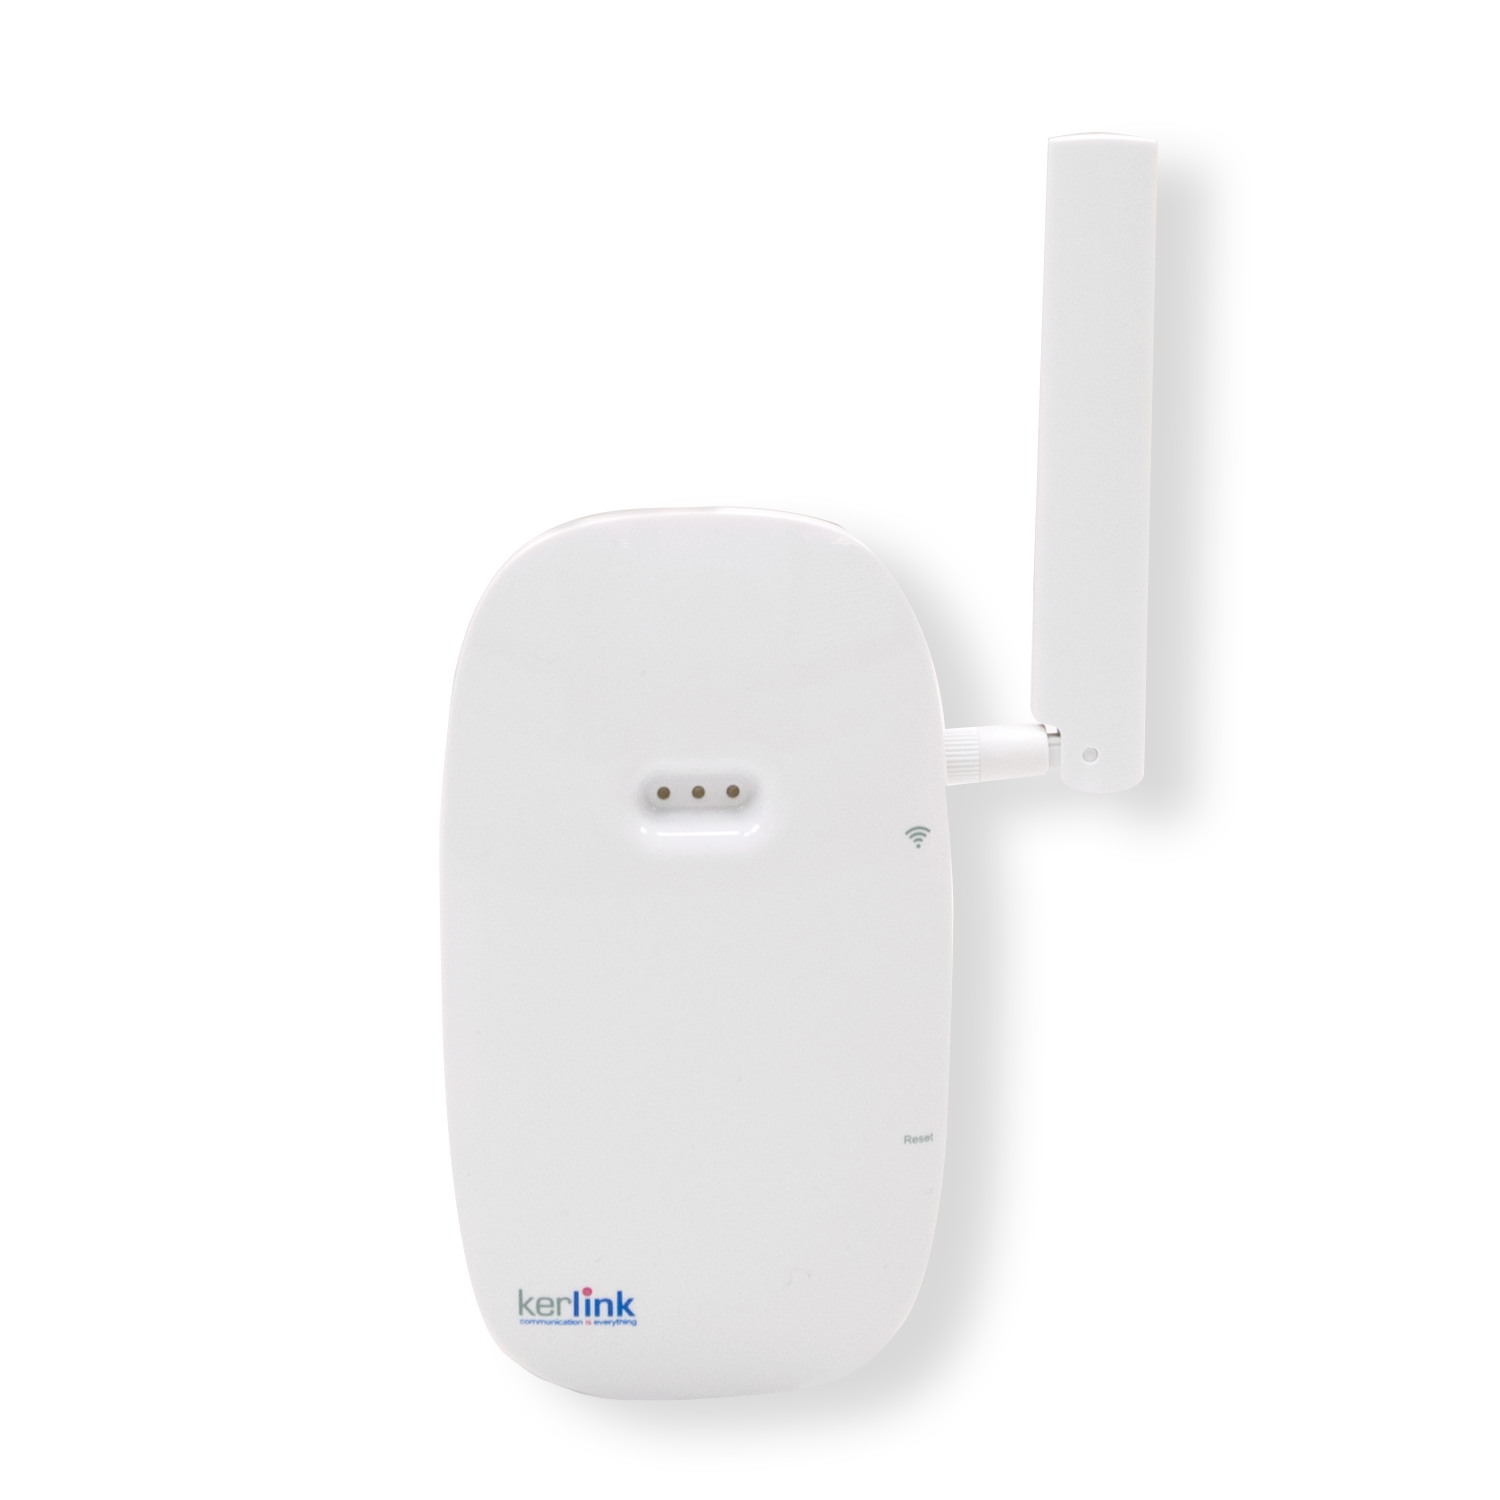
\includegraphics[width=0.7\textwidth]{kerlink}}
  \caption{Kerlink Wirnet iFemtoCell}
\end{figure}


\subsubsection{Raspberry Pi Dragino LoRa GPS Hat}
Dragino LoRa/GPS Hat er en hat lagd lagd for å omforme en Raspberry Pi om til en LoRaWAN gateway. Hatten settes på GPIO pinnene og skrus fast, for så å konfigureres opp. Denne løsningen er en billig måte å teste LoRaWAN løsninger på, som en tilleggsfunksjon vil det kunne kobles opp for GPS posisjonering. Dragino LoRa/GPS Hat kommer med ferdig konfigurerte bølgelengder som avhenger av geo lokasjonen den skal plasseres i. Europas frekvens er 863 til 870 MHz, avvik fra dette vil være ulovlig. 

Rekkevidden for Dragino LoRa/GPS Hat er sammenlignbar med iFemotCell, selv om prisen er betydelig lavere. Dragino LoRa/GPS Hat er også den letteste og mest plassbesparende løsningen på LoRaWAN gatewayer som er tatt med i vurderingen. Dragino LoRa/GPS Hat kommer også med åpen kildekode, og et aktivt miljø av utviklere på nett. Om alt dette tas i betraktning er Dragino LoRa/GPS Hat det beste alternativet for vår lab da det er den mest åpne, og rimeligste plattformen. Det er også mulig å plassere Dragino LoRa/GPS Hat innendørs, og koble den opp og ned lettere om det skulle være ønskelig.

\begin{figure}
  \centering
    \reflectbox{%
      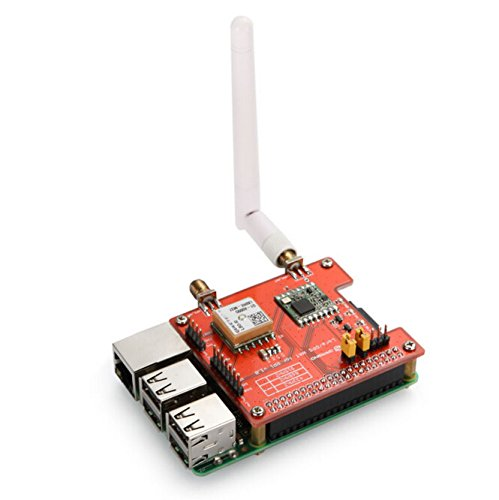
\includegraphics[width=0.7\textwidth]{draginohat}}
  \caption{Raspberry Pi Dragino LoRa GPS Hat}
\end{figure}

\subsection{Sensorer}

\subsubsection{PIR Sensorer}
En PIR sensor er en sensor lagd for å registrere bevegelser, denne typen sensor brukes ofte for å utløse kameraer og for telling av varer som passerer på rullebånd. PIR sensorene på IoT labben er levert av SEEED, og tilkobles ved hjelp av Grove kabler. Årsaken til dette er at Grove kabler enkelt kan kobles til xBee Development Boards. PIR sensorene er digitale og må derfor kobles til DIO4 eller DIO12 på xBee kortene. Når en PIR sensor går høyt gir den en verdi på 1, dersom den går lavt registrerer den 0. En høy verdi betyr registrert bevegelse, lav verdi betyr ingen bevegelse.

\begin{figure}[!ht]
  \centering
      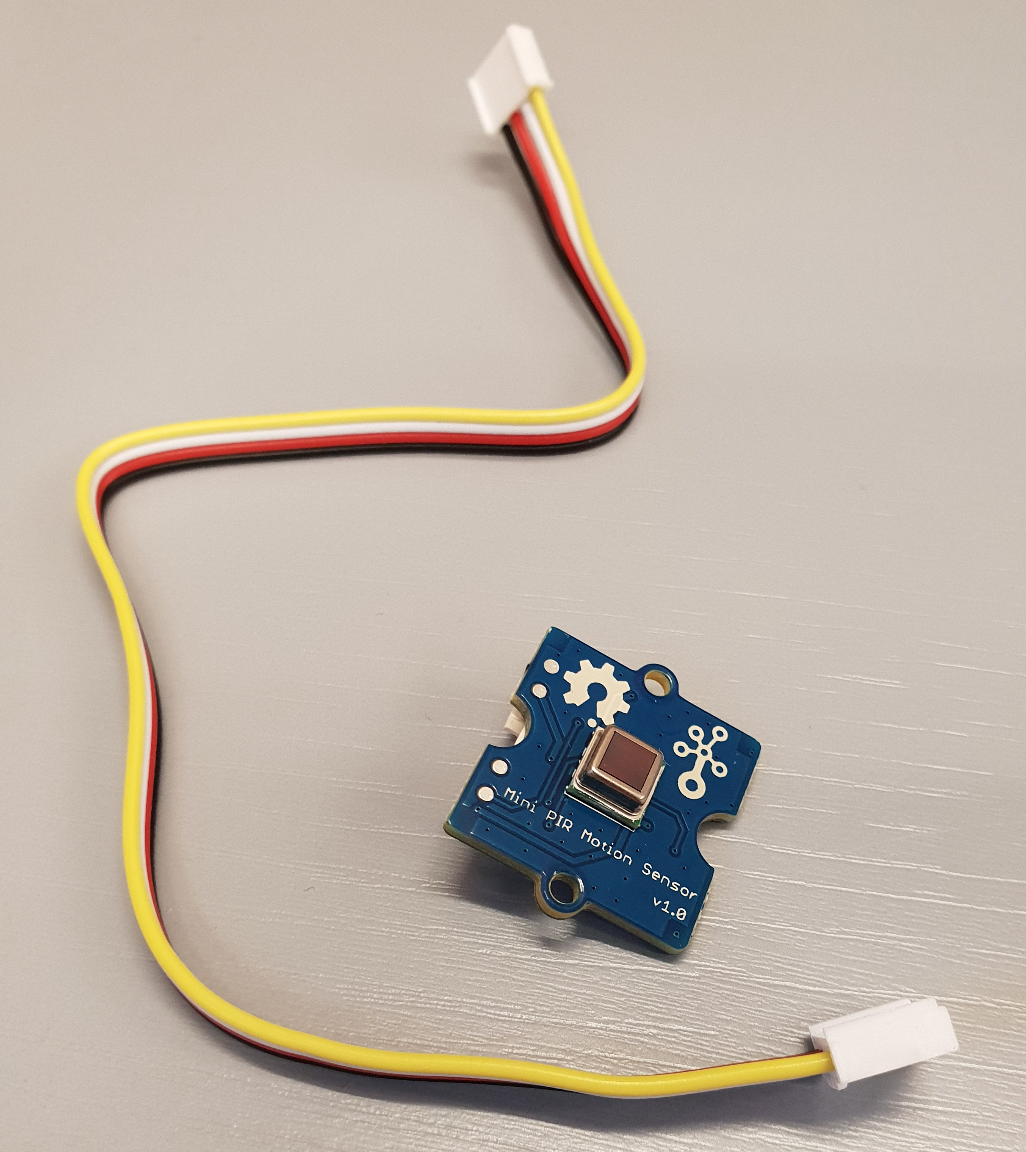
\includegraphics[width=0.4\textwidth]{pirsensor}
  \caption{PIR sensor}
\end{figure}

\subsubsection{Lys Sensorer}
For måling av lys i rommet brukes en lyssensor levert av SEEED, på lik linje med PIR sensorene kobles denne til ved bruk av Grove kabler for rask og enkel tilkobling. Denne sensoren leser inn lysstyrken i lumen, og sender en analog verdi videre. På IoT labben tilkobles sensorene til et xBee Development Board.

\begin{figure}[!ht]
  \centering
      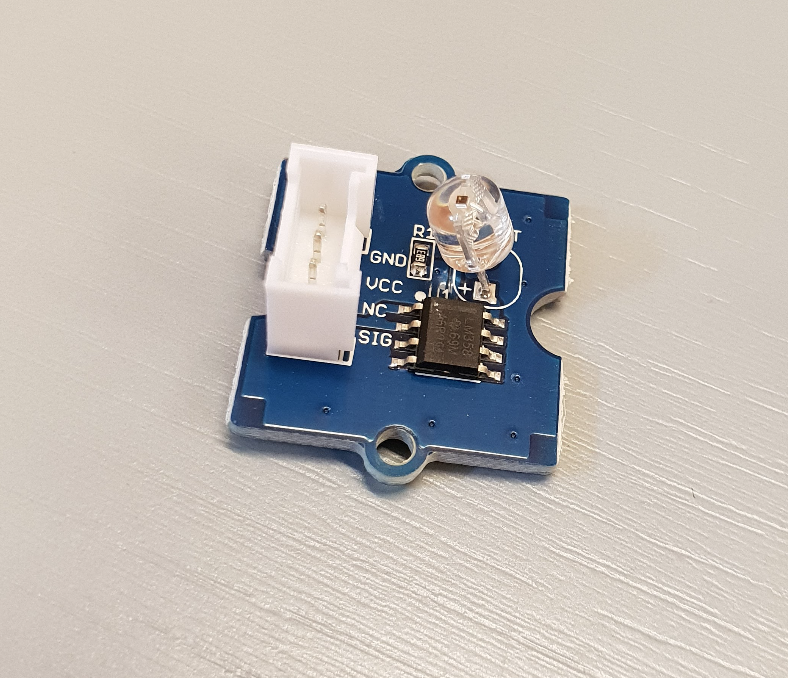
\includegraphics[width=0.4\textwidth]{lyssensor}
  \caption{Lys sensor}
\end{figure}

\subsubsection{Luftkvalitet Sensorer}
Som en del av IoT labben har det vært et ønske å monitorere luftkvaliteten på lab, for å gjøre dette blir en luftkvalitetssensor levert av SEEED brukt, denne tilkobles ved bruk av Grove kabler og kan kobles til xBee Development boards. Sensoren sender analoge verdier av luftkvaliteten. Verdien er en egen enhet utviklet av Grove som baseres på CO, CO2, alkohol, formaldehyde og aceton. Skalaen går fra 0 til 700, og en verdi fra 400 og oppover vil være potensielt skadelig. Normal luftkvalitet vil ligge mellom 100 og 200.

\begin{figure}[!ht]
  \centering
      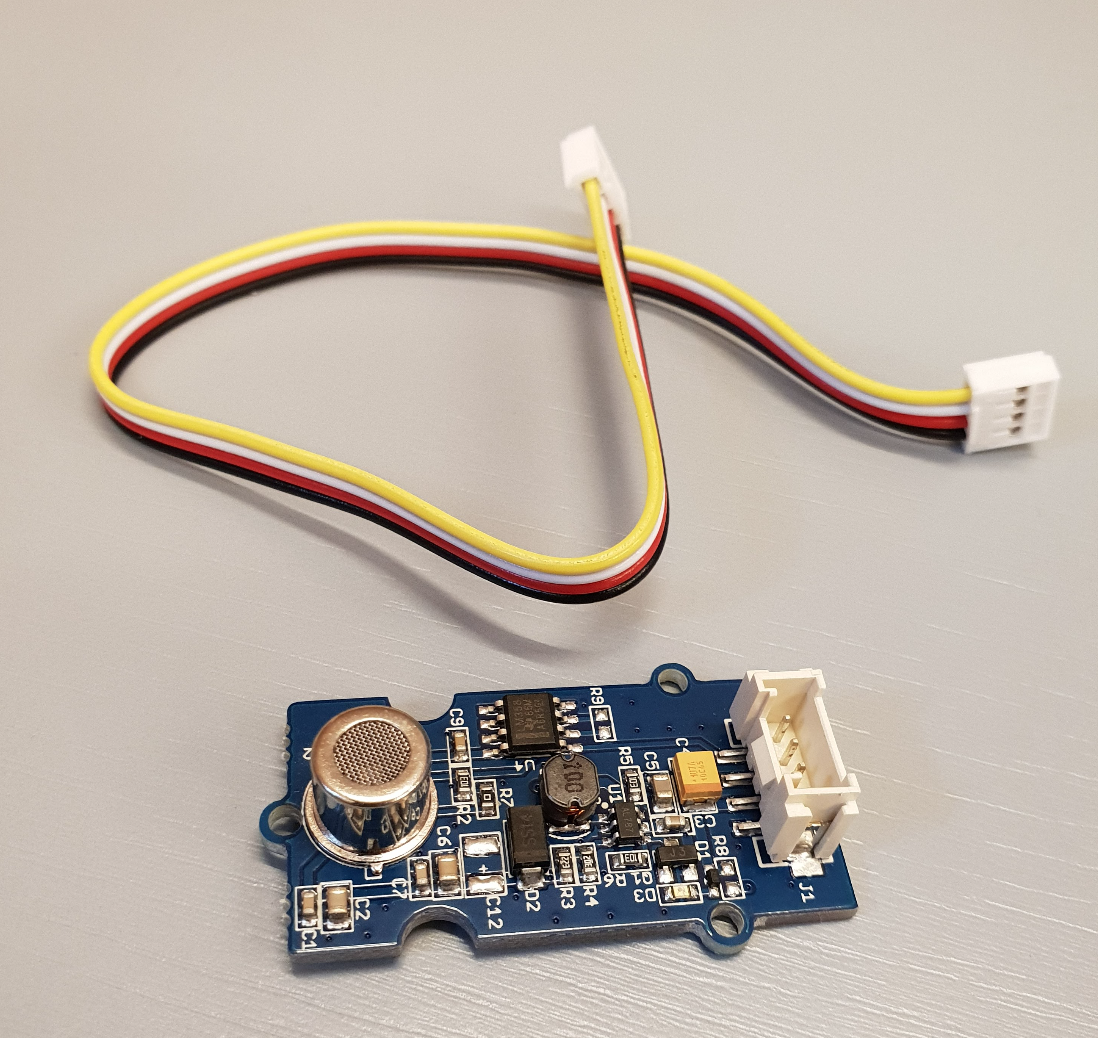
\includegraphics[width=0.4\textwidth]{luftkvalitetsensor}
  \caption{Luftkvalitet sensor}
\end{figure}

%----------------------------------------------------------------------------------------
%   IMPLEMENTASJON PÅ LAB SEKSJON
%----------------------------------------------------------------------------------------

\newpage
\section{Implementasjon på lab}
Videre vil se på oppbyggingen av IoT lab med informasjon om fysisk oppsett av utstyr samt konfigurasjon og kommunikasjon dem imellom. Under er oversikt over hvor alle nettverkene og komponenten samhandler. Vi vil gå nærmere inn på hver enkelt komponent og interaksjon. 



\subsubsection{Node-RED Konfigurasjon}
Node-RED er oppdatert til nyeste versjon på alle Raspberry Pi på IoT labben. Node-RED er også satt op til å starte opp som en del av oppstartsekvensen til Raspberry Pi, på grunn at dette vil man kunne bruke programmet uten å koble til annet en strøm på RPi. Som et sikkerhetsforetak er Node-RED også konfigurert med en administrator bruker og passord. På denne måten vil kun personer med adgang ha mulighet for redigering. 

\subsection{Utstyrplassering og topologi i IoT lab}
\subsubsection{Routere og Switcher}
Router og switch var som nevnt allerede en del av eksisterende kommunikasjon teknologi lab. Utstyret er plassert i rack ved navn “Antarktisk”. 

\begin{figure}[!ht]
  \centering
      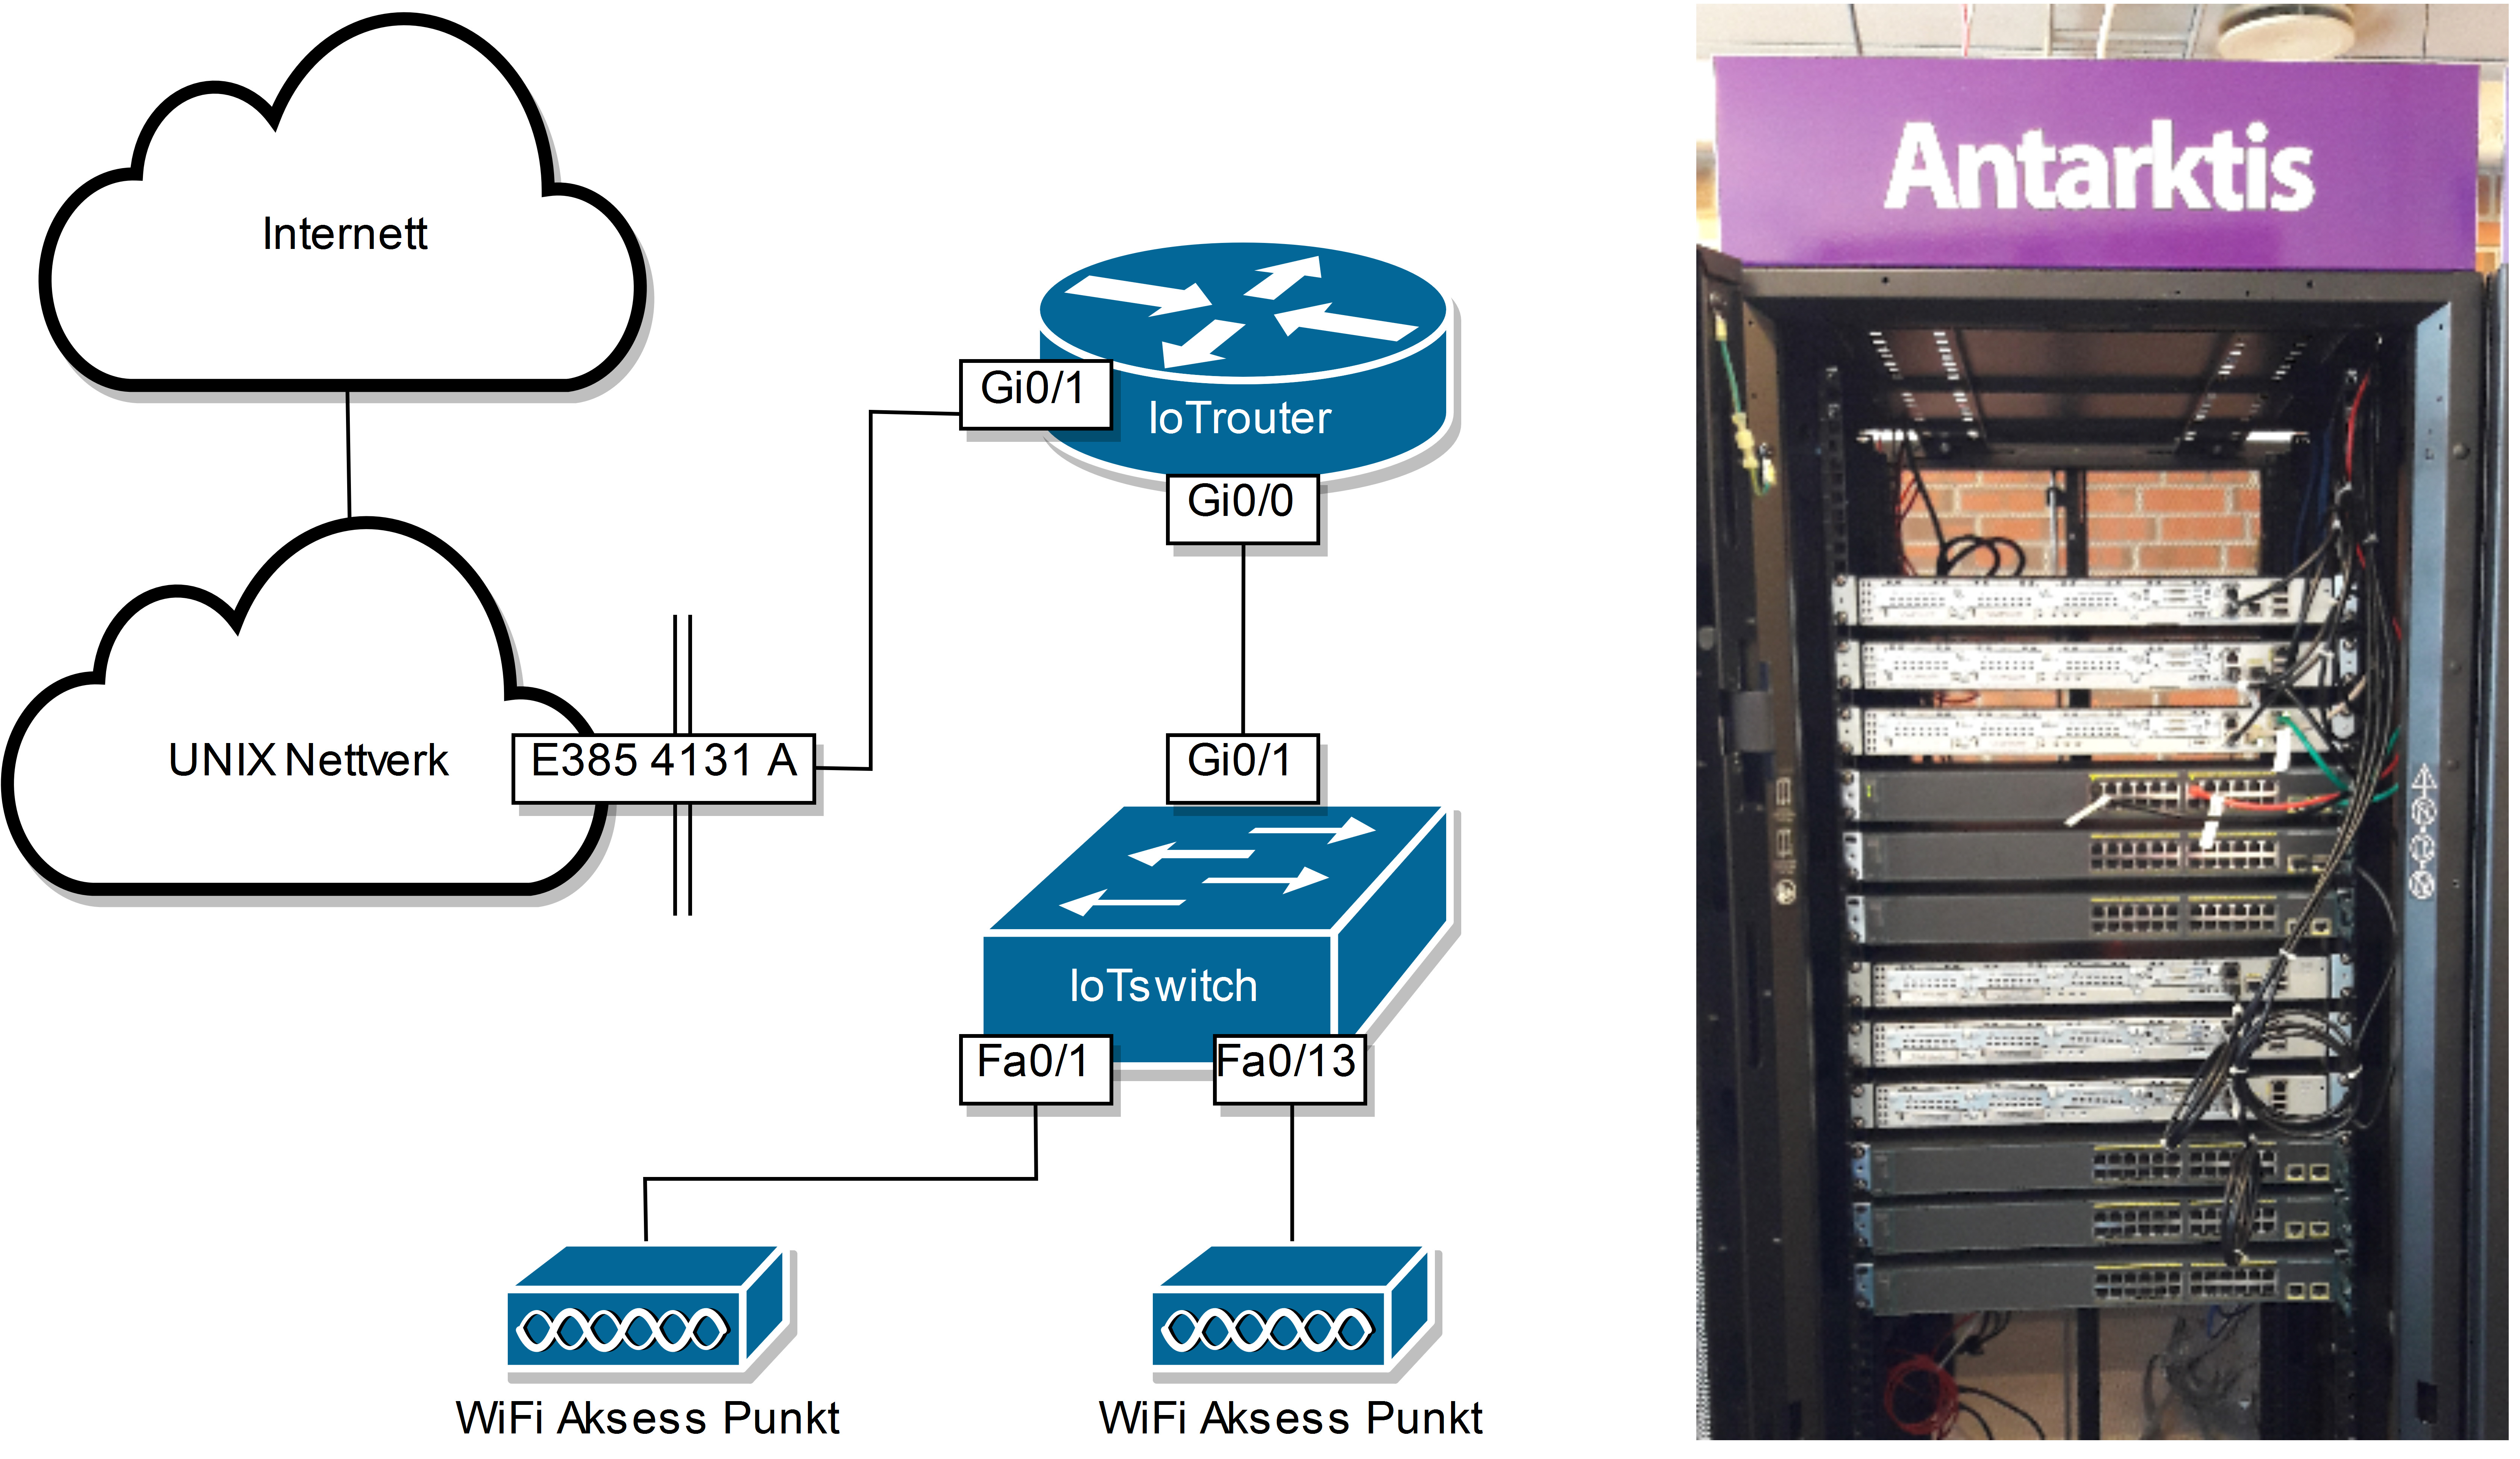
\includegraphics[width=0.95\textwidth]{IoTlabtopologiRouterSwitch}
  \caption{Lag 1 topologi over Router, Switch, WiFi aksess punkt og veggpunkt mot UNIX nettverket}
\end{figure}

Routerens oppgave inkluderer naturlig nok å isolere lab miljøet samt å route trafikk til internett via Universitetets eget interne nettverk, UNIX. I praksis fungerer denne routeren på mange måter som en IoT gateway ved at den aggregerer IoT nettverkene videre mot skyen\cite{iotiot}. 

\subsubsection{Aksesspunkter og Gateways}
På Kommunikasjons teknologi labben har vi valgt å henge opp to WiFi aksesspunkter i taket. Disse er plassert på stiger hengende i taket, og PoE kabel er trukket i kabelstigen fra et stålskap fra Atea som er merket med Antarktis. Dette skapet blir brukt da det ikke er tilgjengelig for studenter. I dette skapet finner vi switchene, ruteren og strømkilden til aksesspunktet. Ved å ha oppsettet slik holdes kommunikasjonsteknologi labben fri for unødvendige kabler og det gjør det lett å koble seg til routere, switcher og aksesspunkt om det skulle være nødvendig. 

Aksesspunktet får både strøm og internett gjennom en Linksys LACPI High Power PoE Injector. Denne strømforsyningen er plassert i samme skap som router og switch, den er hengt opp i skapet for å holde skapet og tilkoblet strøm her for å holde IoT delen av labben så oversiktlig som mulig. Linksys enheten er bygd for å tåle korte strømbrudd, og vil derfor holde aksesspunktet oppe i rundt ett minutt dersom strømmen skulle gå i rommet. Fra switchen er det trukket en 1 meter lang standard cat5 ethernet kabel til Linksys PoE forsyningens Data port. Videre fra Linksys PoE strømforsyningens PoE port er det trukket en 10 meter lang cat5 standard ethernet kabel til aksesspunktet Cisco WAP561. Aksesspunktet benytter seg av Power over Ethernet teknologien, som gir strøm over ethernet kabel. Dette kan være problematisk over dersom distansen er stor fra PoE strømforsyningen, i vårt tilfelle er ikke distansen stor nok til å føre til utfall av tjenester. Alle kabler er merket tydelig med informasjon om hvor de er tilkoblet dersom det skulle være behov for endringer.

Skapene på Kommunikasjonsteknologi labben er plassert midt i rommet, og rett over dem henger kabelstiger. Kabelstiger går til alle hjørner av rommet, dette gav oss muligheten til å henge våre to aksesspunkter i hvert sitt hjørne av rommet, dette vil optimalisere rekkevidden på signalene i hele rommet. Noe som var viktig da skapene med routere og switcher i rommet er lagd av stål, som kunne potensielt ha svekket WiFi signal og lagd dødsoner bak dem. Det har vært svært viktig å sette opp et velfungerende WiFi nettverk da dette har vist seg å være den mest relevante teknologien for undervisning. Det er også den letteste måten å nå ut på internett for andre teknologier som for eksempel ZigBee. 

Som en del av det fysiske oppsettet har vi valgt å ta med Raspberry Pi, dette er fordi den spiller flere roller og er sentral del av oppsettet til flere IoT teknologier. Raspberry Pi enhetene har ikke en fast fysisk plassering der de står og er oppkoblet på Kommunikasjonsteknologi labben, men tas frem dersom man ønsker å teste egne prosjekter eller dersom studenter skal gjøre oppgaver som krever dem. Det vil være lite praktisk å montere dem dersom man skal bytte sensorer, hatter eller koble til skjerm. All programvare som trenges for å utføre lab oppgavene vi har lagt ved er installert og klart til bruk. Det er også vedlagt instruksjoner om hvordan man installerer allt av programvare, oppkobler allt av utstyr og tester om alt er riktig satt opp. Dette har vi valgt å gjøre for å klargjøre labben for utvidelse, og for at studenter skal kunne teste dette på eget utstyr om de ønsker å kjøpe dette. Denne labben er ment å være både for Kommunikasjonsteknologi studenter og studenter som interesserer seg for IoT og ønsker å teste selv.

For å gjøre det lettere for studenter og for implementering av protokoller som MQTT har vi valgt å tildele universitetets Raspberry Pi mikrodatamaskin egne statiske IP-adresser. Det har også som nevnt tidligere blitt avsatt flere IP-adresser om utvidelser av IoT labben blir gjort. Bruk av statiske IP-adresser gjør det også lettere å være sikker på hvilken Raspberry Pi man kobler seg til dersom det brukes SSH for å nå maskinen. Noe som kan være praktisk da man ofte ikke vil ha behovet eller plass til å koble opp en egen monitor, mus og tastatur. 



\subsection{Internett}

\subsubsection{Router og Switch konfigurasjon}
En vil i denne avsnittet ta for seg valg og konfigurasjon på router og switch. Det er tatt hensyn til dagens lab oppsett, krav under utbygging og testing av IoT aspektet i forbindelse med oppgaven samt legge opp til fremtidig utvikling og skalering. Merk at konfigurasjon som er vist i dette avsnittet kun er uttdrag og ikke fullstendig. Dette er for bedre lesbarhet og lettere kunne fremheve valgene som er tatt. 


Uplink interfacet på IoTrouter er GigabitEthernet0/1 og fungerer da som ett WAN interface som når internett via universitets forskningsnett, UNIX. Da vi satte opp router ser vi UNIX hadde ett /23 nett med public ip adresser, 152.94.122.0/23 som blir tildelt via DHCP. Vi trenger derfor ikke sette opp statisk ip adresse på dette interfacet. 


\begin{verbatim}
interface GigabitEthernet0/1
 description ### Connectivity to Unix Network ###
 ip address dhcp
 ip nat outside
!
\end{verbatim}

Det vil følgelig være behov for egen adressering og bruk av private IP-adresser. I tillegg ønsket man å holde IoT lab miljø isolert, inkludert UiS sitt forskningsnett UNIX. Det naturlige var derfor å sette opp NAT mellom IoT lab og UNIX.


\lstset{breaklines=true}
\begin{verbatim}

interface GigabitEthernet0/0.110
 description ### Trunking for Vlan 110 ###
 encapsulation dot1Q 110
 ip address 192.168.1.1 255.255.255.0
 ip nat inside
 !
interface GigabitEthernet0/0.120
 description ### Trunking for Vlan 120 ###
 encapsulation dot1Q 120
 ip address 192.168.2.1 255.255.255.0
ip nat inside
!
ip nat inside source list 100 interface GigabitEthernet0/1 overload
!
access-list 100 permit ip 192.168.1.0 0.0.0.255 any
access-list 100 permit ip 192.168.2.0 0.0.0.255 any

\end{verbatim}


Routeren innehaver også en annen viktig funksjon i at den er DHCP server for IPv4 og IPv6 nettverkene. Vi har her brukt UiS sine DNS servere. Det er også besluttet å reservere de første 30 adresser, inkludert gateway adresse til statisk adressering som kan være veldig nyttig om det skulle være behov for hardkode en ip adresse på en enhet. Lease tiden er satt til 24 timer som er standardinnstillingen hos Cisco. Det er satt en fast DHCP\cite{dhcplease} lease til den en Raspberry Pi, 192.168.1.25. Den er reservert ved client id som her består av 01 + mac adressen. 

\lstset{breaklines=true}
\begin{verbatim}
ip dhcp excluded-address 192.168.1.1 192.168.1.30
!
ip dhcp pool IoT_IPv4_A
 network 192.168.1.0 255.255.255.0
 default-router 192.168.1.1
 dns-server 152.94.1.39 152.94.1.11
 lease 1
!
ip dhcp pool RaspberryPI-static
 host 192.168.1.25 255.255.255.0
 client-identifier 01b8.27eb.fc65.c3
!
\end{verbatim}


Universitet i Stavanger har pr i dag ikke tatt i bruk eget IPv6 adresse prefix. En har derfor generert en egen Unique local adresse ut i fra FC00::/7 som definert RFC4193\cite{rfc4193d}. Vi setter L bit til 1 da dette er en lokalt definert adresse som beskrevet i teori delen rundt IPv6. En ender da opp med prefix FE00 (1111 1110 0000 0000). Videre har en valgt en subnet ID for på den måten vil en ha bedre kontroll på hvilke nettverk de ulike IoT enhetene er på ut fra ipv6 adressen. For nettverk A med subnet 000A blir IPv6 adresseområdet som følger;

\lstset{breaklines=true}
\begin{lstlisting}
Prefix/L bit:   FE00
Global ID:      0000 0000
Subnet ID:      000A
CID:            FE00:0:0:A::/64
\end{lstlisting}
\lstset{breaklines=true}

En har valgt å sette opp en stateful DHCPv6 server. Grunnen til dette er så det vil være lettere å oversikt over hvilke nett de ulike IoT enheter tilhører basert på ip adressen. Det gjør det også lettere å undersøke trafikk i alle ledd med tanke på DHCP bindinger på server og forventede adresser i pakker fanget opp av for eksempel wireshark. DHCPv6 serveren er satt med Google sine DNS servere da UiS ikke har egne for IPv6. Lease tiden er satt til 24 timer i likhet med DHCP for IPv4. 

\lstset{breaklines=true}
\begin{verbatim}
ipv6 dhcp pool IoT_IPv6_A
 address prefix FE00:0:0:A::/64 lifetime 86400 86400
 dns-server 2001:4860:4860::8888
 dns-server 2001:4860:4860::8844
 domain-name IoT-IPv6-A.com
!
\end{verbatim}

Vi aktiverer DHCPv6 på interfacet med rapid commit. Det vil si at den tildeler ip i 2 steg anmodning og svar i motsetning til normale 4 steg; anmodning, advisere,  forespørsel og svar. Ettersom dette er ett forholdsvis lukket og isolert nett er vi ikke bekymret for DHCP hammering eller andre former for misbruk av DHCPv6 server. Videre er det tildelt et link-local og Unique local adresse fra vårt tidligere definerte adresseområdet. I og med at dette skal være en stateful DHCP server, settes både M(anaged) og O(ther) bit til 1. Router advertisment er satt til 10 sekunder. Dersom en ønsker å legge av et antall adresser til statisk adressering kan en sette ett prefix til no autoconfig på interfacet. For eksempel vil FE00:0:0:A:1111::/80 være reservert for auto adresering ved ipv6 nd prefix FC01:0:0:A:1111::/80 infinite infinite no-autoconfig. 


\lstset{breaklines=true}
\begin{verbatim}
interface GigabitEthernet0/0.110
 description ### Trunking for Vlan 110 ###
 encapsulation dot1Q 110
 ipv6 address FE80::1 link-local
 ipv6 address FE00:0:0:A::1/64
 ipv6 enable
 ipv6 nd managed-config-flag
 ipv6 nd other-config-flag
 ipv6 nd advertisement-interval
 ipv6 nd ra interval 10
 ipv6 dhcp server IoT_IPv6_A rapid-commit
!
\end{verbatim}
\lstset{breaklines=true}

I ethvert nettverk er det en god ide å ha presis og synkron tid mellom utstyr til blant annet timestamps og logger. Til dette bruker vi NTP \cite{ntpwebsite}, forkortelse for Network Time Protocol. NTP er meget utbredt protokoll som støtte på tvers av de aller fleste plattformer. Eksempelvis har vi som kjent benyttet Rasberry Pi i store deler av oppgaven.  Denne har ikke en innebygd Real Time Clock (RTC) og er derfor helt avhengig av å hente tid fra annet sted i nettverket for hver oppstart med mindre det blir innstallert en egen RTC modul. Da tanken er at den alltid skal være tilkoblet IoT nettverket besluttet man  å heller ha en egen NTP server internt. Som en ser i figuren under benytter vi en åpen NTP tjeneste, NTP pool project samt UiS sin egen NTP server. 



\lstset{breaklines=true}
\begin{figure}[!ht]
  \centering
      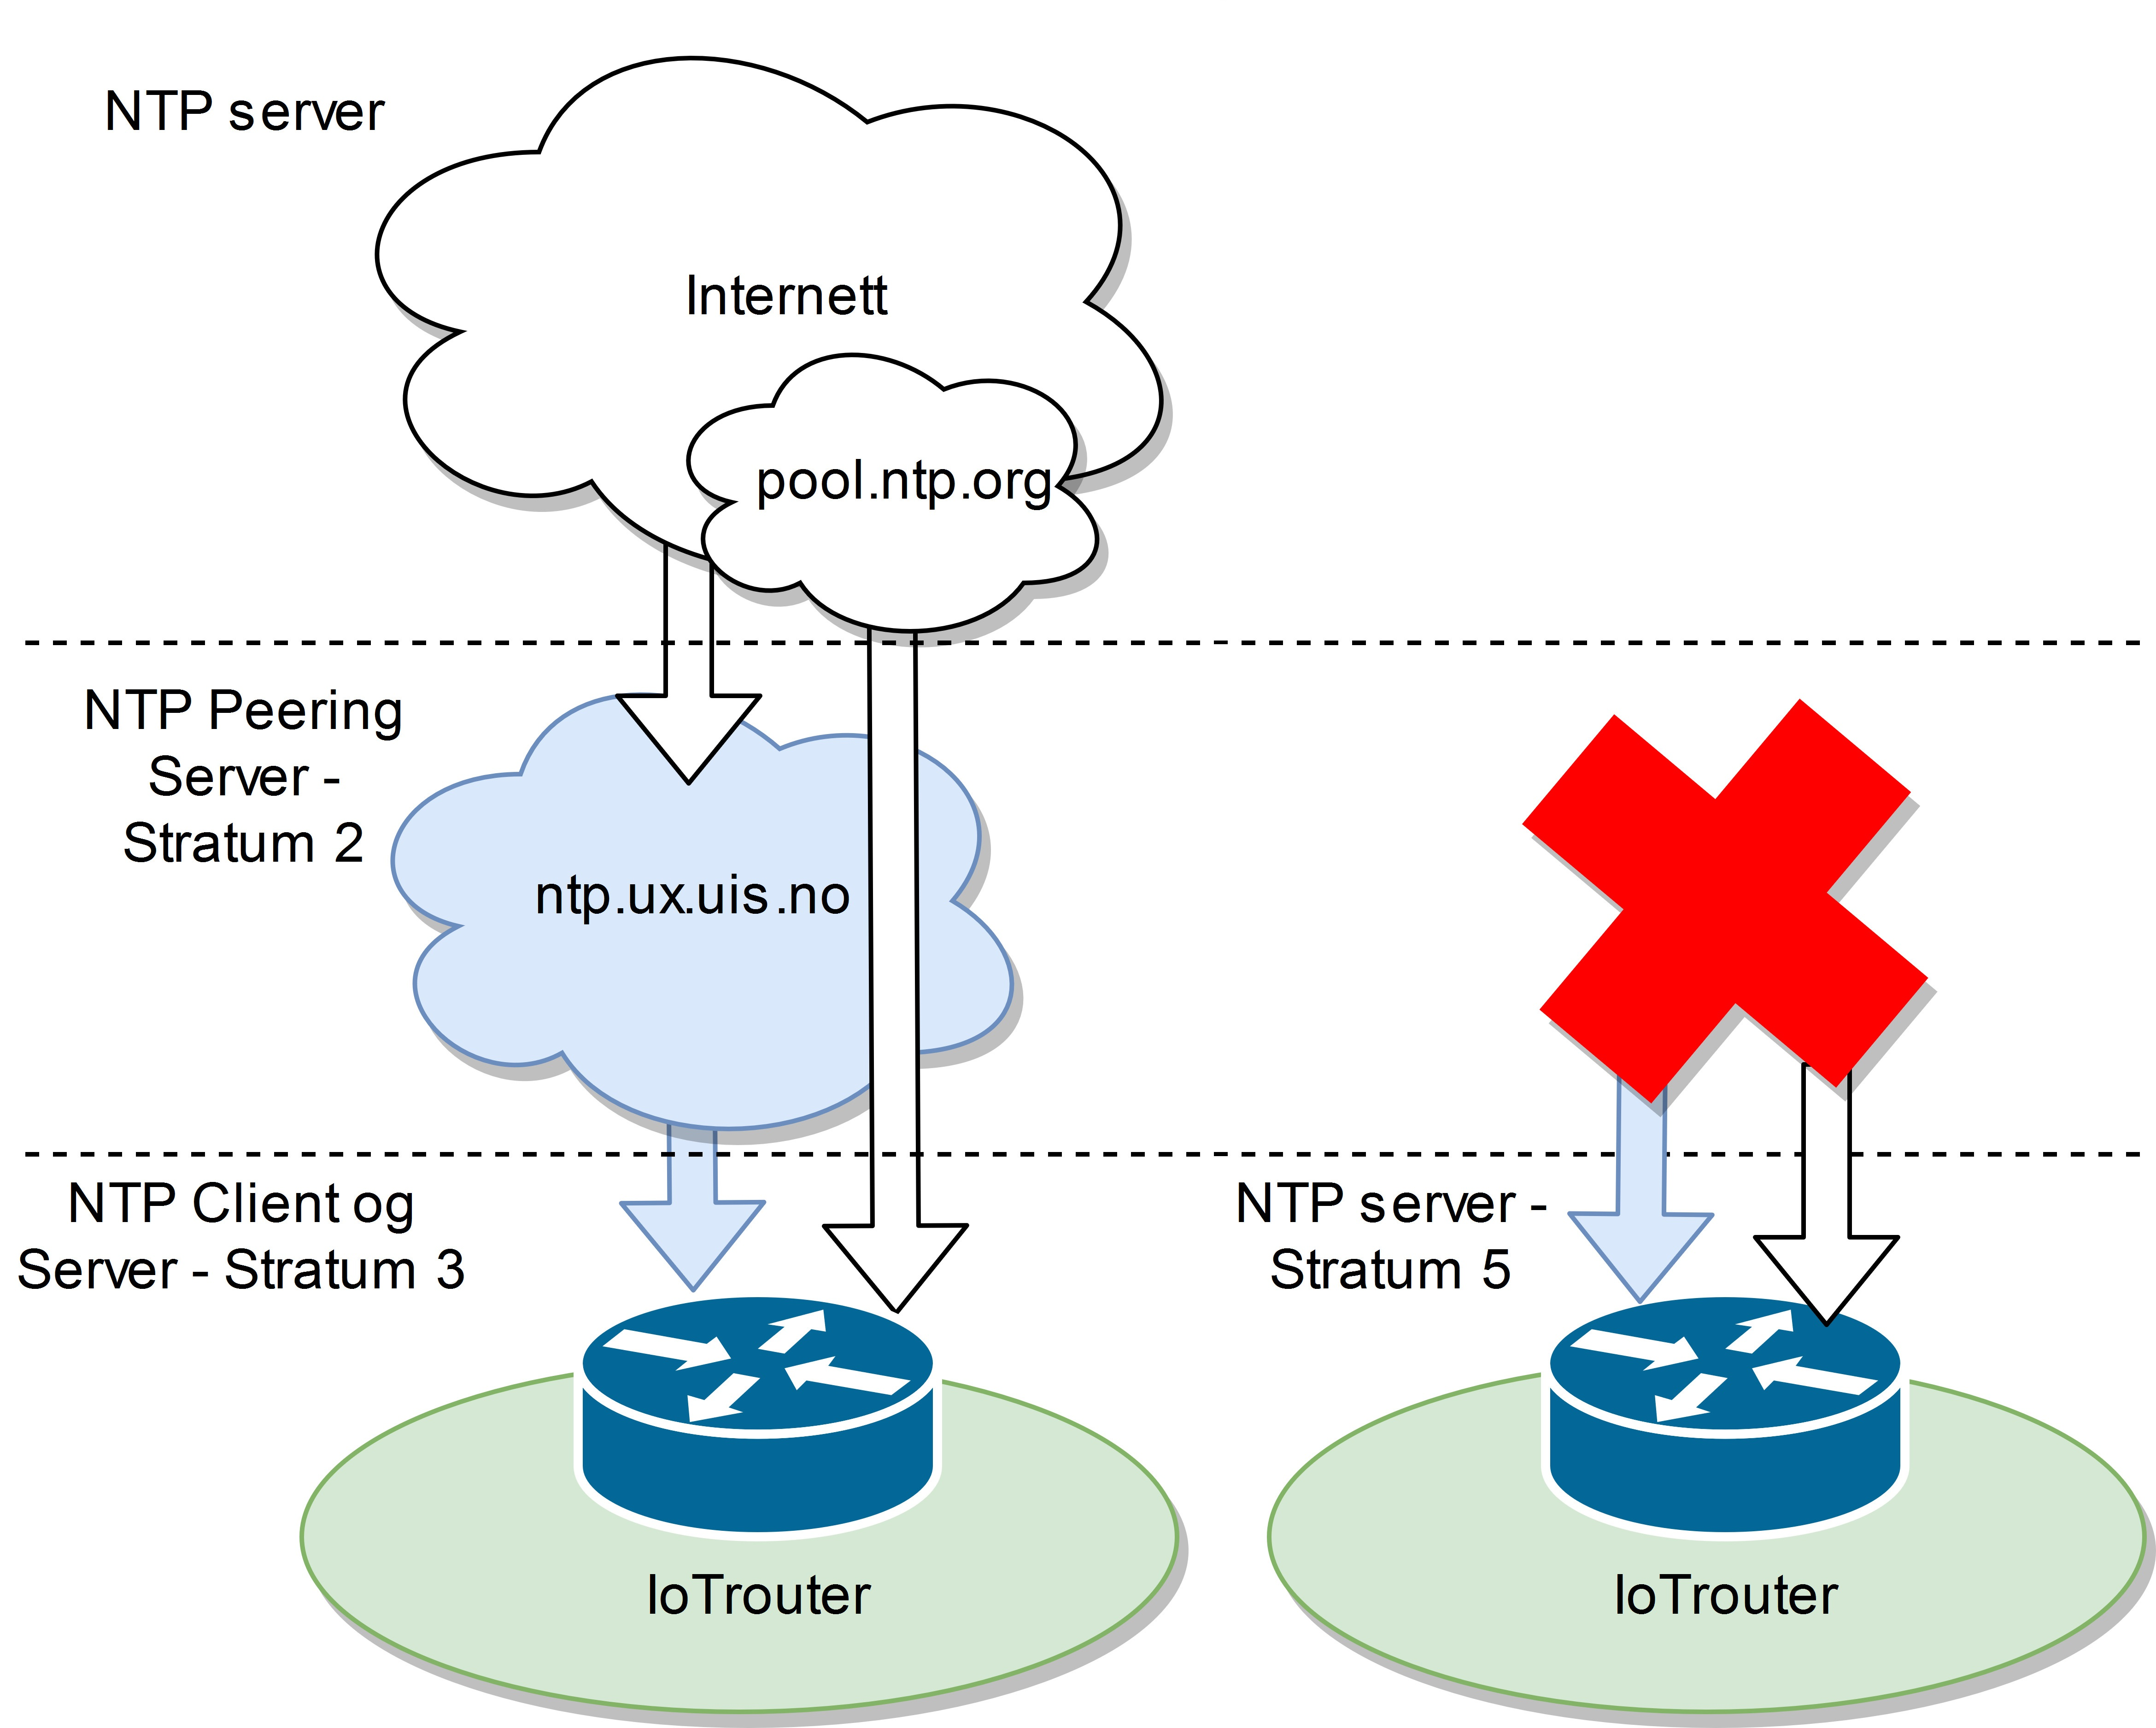
\includegraphics[width=0.7\textwidth]{NTP}
  \caption{Nettverksdiagram over NTP server, peering og klienter. Høyre side illustrerer dagens oppsett mens venstre viser ett isolert IoT lab miljø med IoTrouter satt som "orphan" med stratum 5}
\end{figure}

\lstset{breaklines=true}
\begin{verbatim}
IoTRouter#
ntp orphan 5
ntp peer ntp.ux.uis.no source GigabitEthernet0/1
ntp server pool.ntp.org prefer
!
\end{verbatim}

Switchen har uplink til router på gi0/1. Komtek labens 2 WiFi aksesspunkt er også tilkoblet hver sin Fast Ethernet port. Til dette er det satt opp to vlan, ett til hvert nett. Det er også satt opp et vlan interface til hver, hovedsaklig til testing. Det er allokert 12 porter til hvert nettverk på switchen. De som pr idag ikke bruk og er satt i shutdown.

\begin{verbatim}
interface GigabitEthernet0/1
 description ### Trunk port til router ###
 switchport trunk native vlan 999
 switchport trunk allowed vlan 110,120
 switchport mode trunk
!
interface FastEthernet0/1
 description ### Access point for vlan 110 ###
 switchport access vlan 110
 switchport trunk native vlan 999
 switchport trunk allowed vlan 110
 switchport mode trunk
 switchport port-security mac-address sticky
!
\end{verbatim}


\newpage
\subsubsection{UNIX nettverket}

Med formål som Universitets forsknings nett med begrenset tilgang og tiltenkt bruksomårdet kan det sies være ett relativt lukket nettverk. En har da begrenset med dokumentasjon og endringsmuligheter og har måtte tilpasset IoT laboratoriets nettverk rundt det eksisterende UNIX nettverket. Det vil forekomme noe repetisjon men en vil for ordens skyld gå i gjennom samhandling mellom IoTlab med underliggende nettverk og UNIX. 

\begin{figure} [!ht]
  \centering
      \includegraphics[width=0.7\textwidth]{unixnett}
  \caption{Oversikt over samhandling med UNIX}
\end{figure}


Det er ikke blitt tildelt IP-adresse fra 152.94.122.0/23 statisk men via DHCP. Ulempen er da at man ikke har forutsigbarhet på hvilke ip adresse interacet har. Det er pr i dag ikke nødvendig men for dokumentasjon og eventuelle fremtidige prosjekter hadde en fast IP-adresse vært å foretrekke. En har fått oppført ett A record på UiS sine DNS servere. 

\begin{verbatim}
komtek-iot-lab.ux.uis.no    A    152.94.122.52
\end{verbatim}

Dersom DHCP server har mulighet til å gjøre ett DNS oppslag etter DHCPDISCOVER fra klienten og før DHCPOFFER er det gjerne mulig å bruke dette som en type reservasjon. Den beste løsningen for fast ip vil likevel være å reserve en IP-adresse mot client-id, som typisk vil være mac-adressen på interfacet. 

\subsubsection{IPv6 ut mot internett}
Som tidligere beskrevet i rapporten har vi et Unique Local IPv6 nett, FC00:0:0:A::/64. Det har blitt utført undersøkelser for å se om det er mulig å benytte dette IPv6 nettverket utad mot internett via universitets nettverk eller mot andre IPv4 nett. 

Det er mulig skape en tunnel fra et IPV6 nettverket til ett annet via et IPv4 nett ved å legge pakkene i en IPv4 header. Metoden kalles 6to4\cite{rfc3056} men navnet kan være litt misvisende i at en 6to4 tunnel ikke går fra et IPv6 nettverk over til IPv4 men derimot mellom 2 ulike IPv6 nettverk via et IPv4 nettverk. Dette oppfyller ikke våre behov for ett IPv6 til Ipv4 transaksjon. 

En av de første metodene i forbindelse med migrering fra IPv4 til IPv6 er NAT-PT introdusert i RFC2766\cite{rfc2766}. Dette har senere blitt ansett som utilstrekkelig\cite{rfc4966} og er for det meste noe som bransjen gått bort ifra. NAT-PT er heller ikke støttet av lisens nivået vi har på routeren. 

Arvtageren til NAT-PT er NAT64 og DNS64, først introdusert i  RFC6146 publisert i 2011\cite{rfc6146}. NAT64 kommer i 2 varianter, stateful og stateless. En har valgt å fokusere på stateful av samme årsaker som vi benytter stateful DHCPv6. I tillegg støtter ikke stateless 1:N ved overload. Stateful vil si at NAT64 oversetteren, i dette tilfellet IoTrouter, holde styr på alle adresser som blir oversatt til og ifra. Dette er på mange måter tilsvarende det som skjer med NAT44 foruten ett viktig konsept. NAT64 skiller ikke mellom inside og outside noe som er forståelig når en ser på formålet til NAT64 kontra NAT44. Hensikten med NAT64 er å muliggjøre kommunikasjon mellom ett IPv4 og IPv6 nettverk mens NAT44 først og fremst er å øke antall ip adresser ved bruk av private, ikke-rutbare adresser bak en offentlig rutbar en. Det er verdt å merke seg denne forskjellen i designet da vårt IPv6 nettverk minner mest om sistnevnte, altså ikke-rutbare IPv6 adresser bak rutbare IPv4. Dette er noe som ikke er NAT64 sin primærfunksjonen til forskjell fra NAT44\cite{rfc1631}. For å illustrere konseptet satte vi opp en statisk NAT64 mellom IPv4 og IPv6 nettverket i lab.

\begin{figure} [!ht]
  \centering
      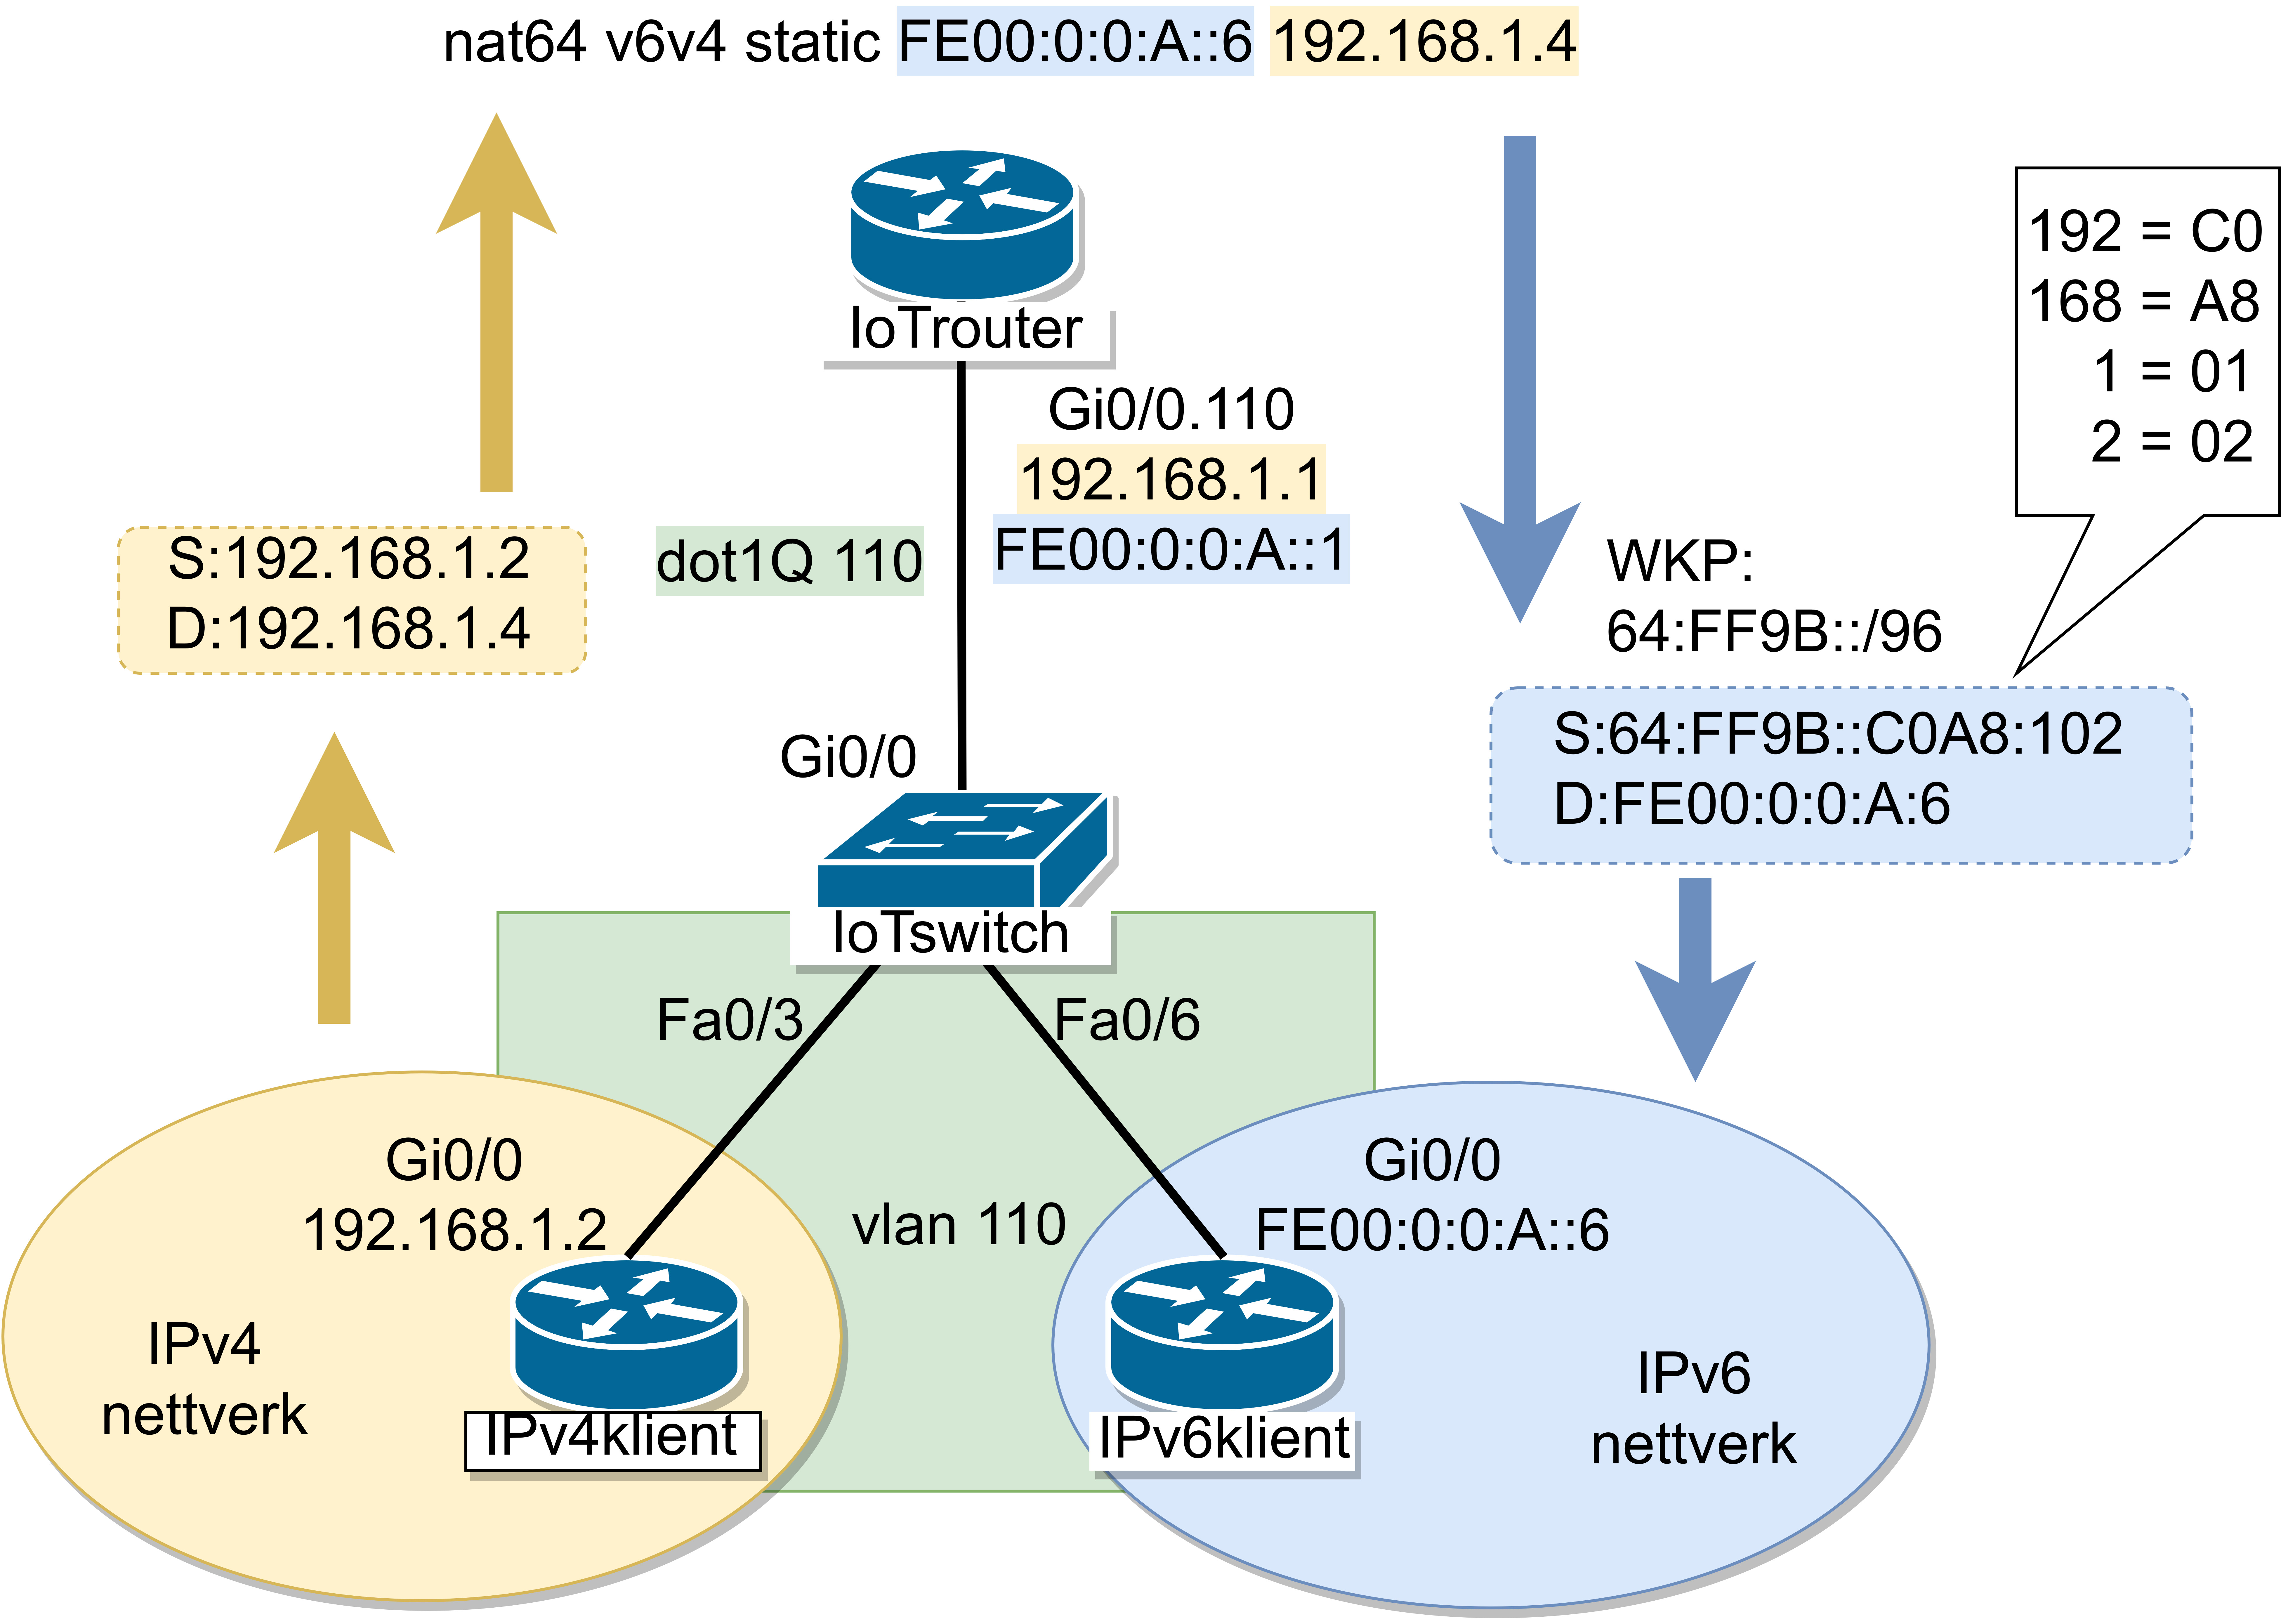
\includegraphics[width=0.95\textwidth]{statisknat64}
  \caption{Statisk NAT64 mellom FE00:0:0:A::6 og 192.168.1.4 illustrerk med oversettelse fra v4 til v6. D: = Destination og S: = Source. WKN = Well Known Prefix}
\end{figure} 

Under ser en relevant konfigurasjon på IoTrouter. I vår topologi er det kun dette subinterfacet som foretar oversettelsen i og med at begge nettverkene henger bak det. 

\begin{verbatim}
IoTRouter#
interface GigabitEthernet0/0.110
 description ### Trunking for Vlan 110 ###
 encapsulation dot1Q 110
 ip address 192.168.1.1 255.255.255.0
 nat64 enable
 ipv6 address FE00:0:0:A::1/64
!
nat64 v6v4 static FE00:0:0:A::6 192.168.1.4
!
\end{verbatim} Videre ser en at IPv4klient kan nå IPv6klient med 192.168.1.4 og vica versa med 64:FF9B::C0A8:102.

\begin{verbatim}
ipv4klient#ping 192.168.1.4
Type escape sequence to abort.
Sending 5, 100-byte ICMP Echos to 192.168.1.4, timeout is 2 seconds:
!!!!!
Success rate is 100 percent (5/5), round-trip min/avg/max = 1/1/4 ms

ipv6klient#ping 64:FF9B::C0A8:102
Type escape sequence to abort.
Sending 5, 100-byte ICMP Echos to 64:FF9B::C0A8:102, timeout is 2 seconds:
!!!!!
Success rate is 100 percent (5/5), round-trip min/avg/max = 1/1/4 ms

IoTRouter#sh nat64 translations
Proto   Original IPv4           Translated IPv4
        Translated IPv6         Original IPv6
--------------------------------------------------------
icmp    192.168.1.2:5028                [64:FF9B::C0A8:102]:5028
        192.168.1.4:5028                [FE00:0:0:A::6]:5028
---     ---                     ---
        192.168.1.4             FE00:0:0:A::6

Total number of translations: 2

\end{verbatim}

Etter videre undersøkelser i ett forsøk på å nå ut på internett fra IPv6 ser vi det i praksis er avhengig av å kunne gjøre oppslag mot en DNS64 og kunne gjøre ett A record (v4) om til ett AAAA (v6) for å ha noen praktisk andvending. Dette gjelder for både stateful og stateless. Statisk oversettelse kan som vist benyttes men vår vurdering er det best å heller prioritere å få et rutbart IPv6 prefix i produksjon og benytte ett subnett av dette.

\subsection{Raspberry Pi}

\subsubsection{Generelt}
En sentral del av vår fremlagte løsning for en IoT Lab er mikrodatamaskinen Raspberry Pi. Tidligere i rapporten har vi sett på den tekniske siden av RPi, i denne delen vil vi argumentere for hvorfor det har vært et godt valg som en sentral komponent i IoT labben vår.
\subsubsection{Python}
For programmering mot Rasperry Pi Sense Hat brukes Python for innhenting av data, her har Raspebrry Pi utviklerne selv lagd biblioteker for henting av data. Her kan det hentes inn data fra accelerometer, magnometer, gyroskop, temperatursensorer og barometer. Det er er også mulighet for skriving av text til Sense Hat 8x8 LED matrise, noe som blir brukt som en del av konsept testing senere i prosjektet. Data hentet inn fra sensorene bearbeides også ved bruk av Python, dette er nødvendig da sensor data som hentes ikke er rundet av. Det er ikke hensiktsmessig for vårt formål å måle temperatur ned til åttende desimal. 

Python benyttes også til sending av data gjennom MQTT protokollen, dette kan gjøres på flere måter. Fellesnevneren er bruk av Paho MQTT biblioteket utviklet av Eclipse Foundation. Ved bruk av dette biblioteket kan man enkelt sette opp en egen lokal MQTT server og sende  data gjennom protokollen på et lokalt nettverk. Det åpner også for muligheten for å sende data ut til internett, da Eclipse Foundationt tilbyr en gratis test klient og server. Her må det påpekes at denne bare er for testing, og data er ikke kryptert. Dette betyr at hvem som helst hvor som helst som abbonerer på temaet man publiserer til kan lytte. Det inneberer og at dersom man har satt opp en klient til å motta fra et tema som henter fra Eclipse Pahos testsider, vil man motta allt som blir sendt gjennom denne kanalen. Detter er derfor ikke å anbefale. 

\begin{lstlisting}[language=R, caption=Sending av tekst ved bruk av Paho MQTT på et lokalt nettverk][h]
import paho.mqtt.client as mqtt
import time

def on_log(client, userdata, level, buf):
	print("log" + buf)

def on_connect(client, userdata, flags, rc):
	if rc == 0:
		print("Connected OK")
	else:
		print("Bad connection Returned code=", rc)

def on_disconnec(client, userdata, flags, rc=0):
	print("DisConnected result code ", str(rc)

broker = "192.168.1.32"
client = mqtt.Client("senseHat")

client.on_connect = on_connect
client.on_disconnect = on_disconnect
client.on_log = on_log

print("Connecting to broker "  + broker)
client.connect(broker)
client.loop_start()
client.subscribe("sense/test")
client.publish("sense/test", "Dette er en test")
\end{lstlisting}

\subsubsection{Node-RED}
Det visuelle programmeringsverktøyet Node-RED kommer installert på Raspberry Pi, det kjører ikke på nyeste versjon, og er ikke tilpasset vårt formål helt enda. Derfor oppdateres RPi til nyeste versjon av Raspian Stretch, og Node-RED oppdateres til nyeste versjon. Det er også installert flere relevante noder som kan brukes av studenter til egne IoT oppgaver. Her er de mest nevneverdige nodene som er installert Node-RED Dashboard, Python Functions, ZigBee rx/tx og Sense Hat noden. Å gjøre dette vil forenkle læringsprosessen og gjøre labben lettere å bruke.


\subsubsection{Mosquitto MQTT Broker}
Mosquitto MQTT Broker er en megler lagd for å gjøre RPi til en server og klient for sending og mottakelse av strømmer fra MQTT protokollen. Mosquitto MQTT Broker er implementert på alle RPi enhetene i IoT labben, og kan brukes som del av fremtidige oppgaver hvor det ønskes å lage egne programmer for sending av MQTT data uten bruk av Node-RED. Mosquitto er utviklet av Eclipse Foundation, og støtter alle typer sending og kryptering ved MQTT. Formålet med denne implementasjonen er at man her enkelt vil kunne skrive egne programmer i for eksempel Python, hvor det hentes og publiseres data som trenger mer bearbeiding, og hvor det ikke er ønskelig å bruke et visuelt programmeringsverktøy.

\subsubsection{Azure Cloud MQTT Broker}
Under oppgaven ble Azure Cloud MQTT Broker vurdert som en alternativ, denne megleren er tilkoblet skyen til Microsoft Azure og muliggjør henting av MQTT data fra hvor som helst i verden da den er på Internett. Azure Cloud MQTT Broker er trygg og populær tjeneste for styring av IoT, og kombineres ofte med Azure IoT Hub. Azure Cloud MQTT Broker har ikke blitt konfigurert på RPi enhetene på IoT labben for å holde lab miljøet så lukket som mulig. Det er mulig for studenter å sette dette opp på egne maskiner for testing av egne prosjekter.

\subsubsection{Andre Internettbaserte MQTT Broker}
Som en del av testprosessen for MQTT har HiveMQ blitt brukt i sending av temperatur data. HiveMQ er en nettbasert megler som tilbyr gratis testing av MQTT sendinger. Testingen ble gjort gjennom HiveMQ Websocket klient som et bevis på at konseptet virker.

\begin{table}[h!]
	\centering
	\caption{Detaljer testing mot HiveMQ}
	\label{HiveMQ}
	\begin{tabular}{|l|l|}
		\hline
		\textbf{Host:}  & broker.hivemq.com \\ \hline
		\textbf{Port:}  &  1883\\ \hline
		\textbf{Websocket Port: }& 8000 \\ \hline
		\textbf{ClientID: } & Genereres automatisk for å hindre brukt til annet en testing \\ \hline
	\end{tabular}
\end{table}


\subsection{ZigBee}

\subsubsection{Nettverks konfigurasjon}
Konfigurering av IoT labbens ZigBee nettverk gjøres ved bruk av XCTU, et program for styring og konfigurering av xBee moduler. 

\begin{table}[htbp]
\centering
\begin{tabular}{|l|p{0.8\linewidth}|}
\hline
\multicolumn{1}{|c|}{\textbf{Parameter}} & \multicolumn{1}{c|}{\textbf{Forklaring}}                                                   
\tabularnewline \hline

\textbf{ID}                                               & Definerer nettverket som en radio vil koble seg til. Dette må være likt for alle radioer på nettverket 
\tabularnewline \hline

\textbf{JV}                                              & Verifiserer om en koordinator eksisterer på samme kanal, den vil delta i nettverk om det finnes, eller forlate om den ikke kan finne koordinator \tabularnewline \hline

\textbf{CE}                                         	& Gir en node rollen som koordinator i nettverket \tabularnewline \hline

\textbf{DH}                                             & Definerer en spesifikk destinasjons adresse, om denne er satt til 0, vil traffikk gå til koordinator. Dette er de 8 første tallene i destinasjonsenhetes MAC-adresse
 \tabularnewline \hline
 
\textbf{DL}                                              & Definerer en spesifikk destinasjons adresse, om denne er satt til 0, vil traffikk gå til koordinator. Dette er de 8 siste tallene i destinasjonsenhetes MAC-adresse 
\tabularnewline \hline

\textbf{NI}                                                  & Gir enheten et navn  som lettere kan leses av mennesker, denne parametern blir ikke brukt i adressering
\tabularnewline \hline

\textbf{AP}                                            		& Tillater API operasjonsmodus
\tabularnewline \hline

\textbf{SP}                                                 & Definerer søvnsyklus
\tabularnewline \hline

\textbf{SM}                                                  & Tillater syklisk sovemodus
\tabularnewline \hline

\textbf{D0 til 12}                                          & Åpner for innhenting av data fra GPIO pinner
\tabularnewline \hline

\textbf{IR}                                                  & Henter inn data fra analoge sensorer ved et gitt tidsintervall, definert ved hexadesimale verdier
\tabularnewline \hline
\end{tabular}
\caption{Tabell over relevante parametere i XCTU og deres betydning}
\label{table:XCTU tabell}   
\end{table}


\subsubsection{Kommunikasjons tester mellom noder}

\begin{figure} [!ht]
  \centering
      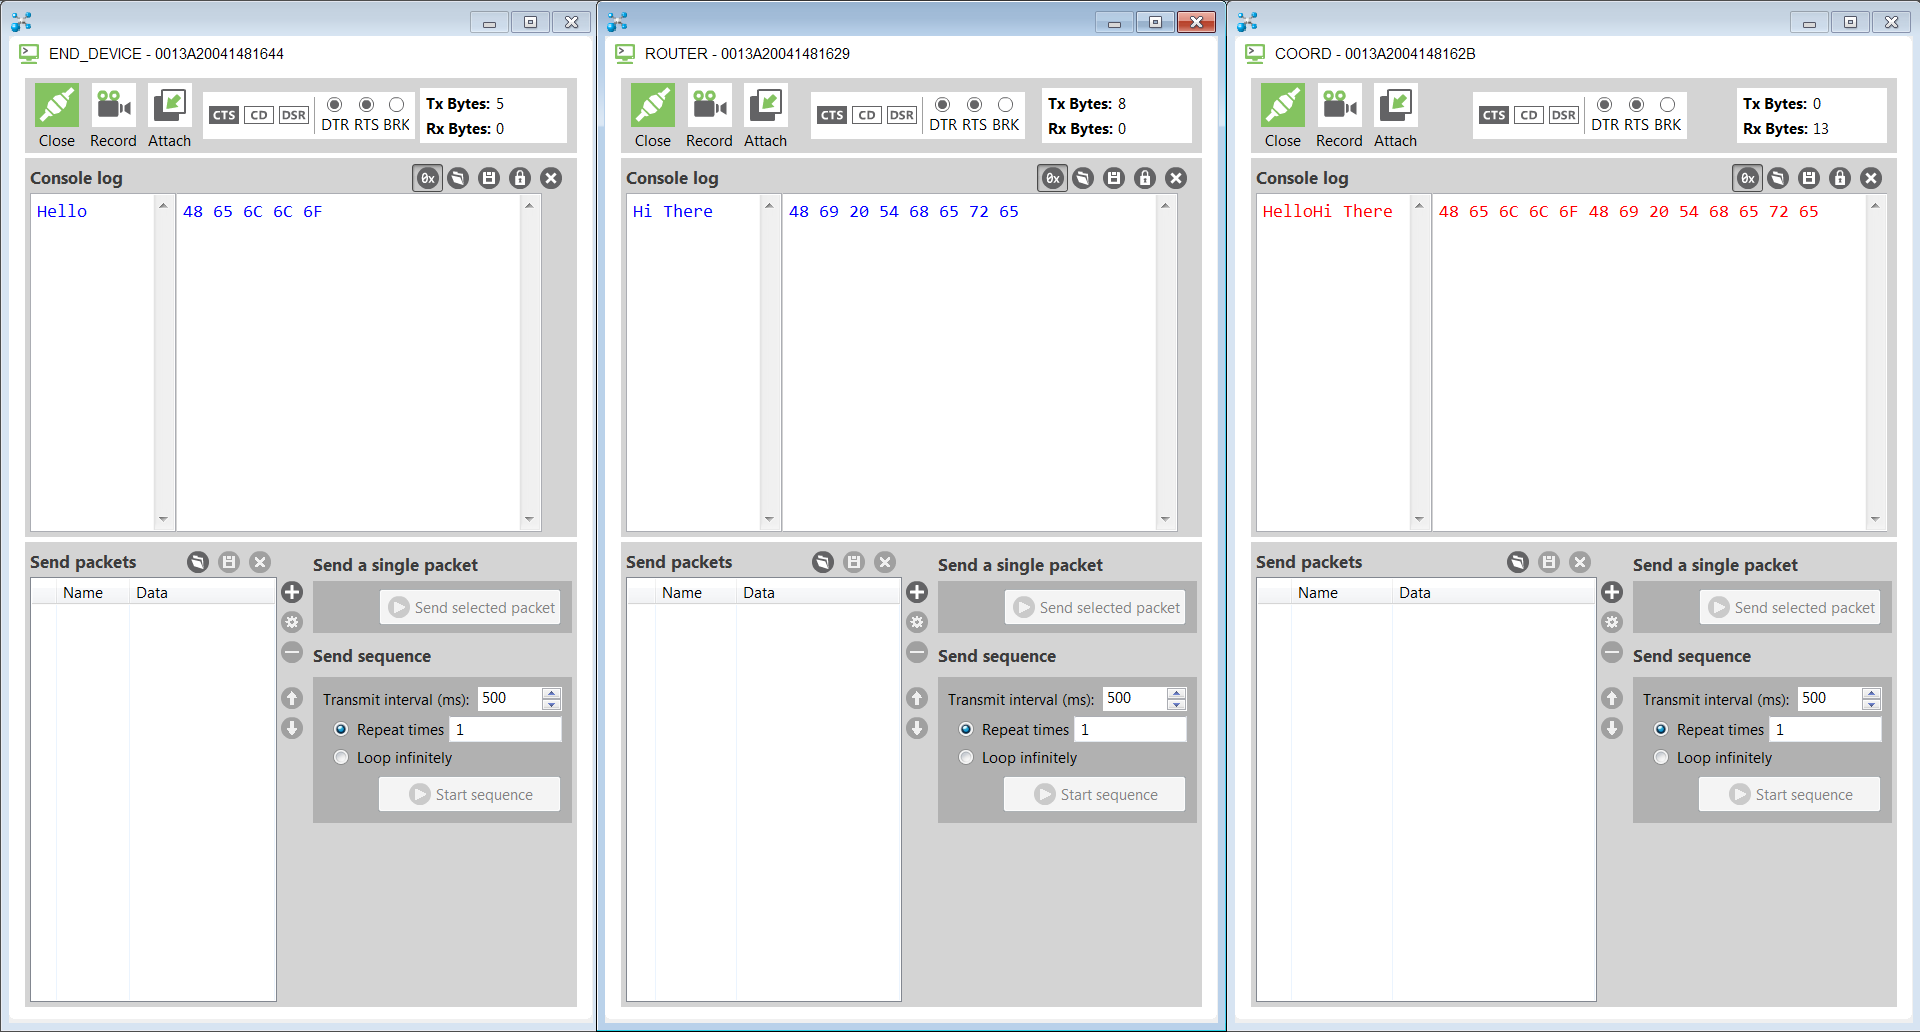
\includegraphics[width=0.95\textwidth]{XBeeFirstHello}
  \caption{Test av kommunikasjon mellom xBee noder i et ZigBee Mesh nettverk}
\end{figure}

Under bygging av ZigBee mesh nettverket har første steg etter konfigurasjonen av nodene i nettverket vært testing av kommunikasjonen mellom forskjellige noder. Å teste ved sending av tekst er den enkleste måte å teste om nettverket fungerer som det skal. Ved å utføre denne testen utelukker man variabler som feil på sensorer, feil konfigurert innhenting av data og feil ved bearbeiding av data. Testing av tekst kommunikasjon er derfor en viktig del av testdrevet utvikling, da det er letteste måte å sende data gjennom nettverket.

Etter mesh nettverket er konfigurert gjennom XCTU, kobles routeren i nettverket og ende noden i nettverket til en datamaskin. Koordinatoren kobles til en annen datamaskin, deretter åpner man XCTU og kobler til enhetene ved å åpne for seriell kommunikasjon. Man kan nå sende tekstmeldinger fra de forskjellige nodene i nettverket gjennom konsollet. Dersom man skriver fra konsollet på koordinatoren vil man få en beskjed på ruteren.

\subsubsection{Innhenting av Sensor Data}
Innhenting av sensordata er en essensiell del av en IoT lab, og en av de mest populære teknologiene for sending av forskjellige typer sensor data er ZigBee. Sending av sensordata gjennom ZigBee er derfor viktig for å holde IoT labben aktuell. ZigBee er også en av de mest brukte teknologiene både i industri og i smart hjem. Sending av sensor data gjennom et ZigBee nettverk er også et naturlig steg videre etter testing med sending av tekstmeldinger er utført.

For innhenting av sensor data fra IoT labbens xBee noder for så å sende data videre i nettverket er det enklest å benytte seg av Grove sensorer som enkelt kan kobles til xBee Development Boards ved en enkel kabel. Som en del av IoT labben i E-472 har universitetet gått til innkjøp av flere forskjellige Grove sensorer for studenter og som en del av selve labben. Under oppkoblingen av ZigBee nettverket og testing av sending av sensor data ble det først testet med analoge sensorer, og deretter digitale. Analoge sensorer gir ut en numerisk verdi som som for eksempel temperatur i celsius, en digital sensor gir ut enten 1 eller 0. En digital sensor kan for eksempel være en infrarød sensor som avgir verdi 1 om den registrerer bevegelse og 0 om den ikke registrerer noe. Ved bruk av sensorene må xBee Grove Development board konfigureres til å hente rett type data fra grove tilkoblingen, dette gjøres i XCTU ved å sette tilkoblingen til lesing av digital eller analog. For digitale sensorer er det ikke nødvendig å konfigurere mer for å hente data gjennom porten. Analoge sensorer krever konfigurering av innhentings intervaller, dette er en egenskap som må konfigureres i hovedsak på grunn av strømsparing. Parameteren IR bestemmer hvor ofte analoge data hentes, og kan hente data opp til 5 ganger i sekundet, det anbefales å sette innhenting til omtrent 2 sekunder da oftere innhenting som regel er unødvendig.

Nettverket er konfigurert som et ZigBee mesh nettverk med en koordinator, en ruter og en ende node. Som en del av det ferdige oppsettet er koordinatoren tilkoblet en RPi som mottar data og videresendes til en IoT dashboard for monitorering. Dette vil bli diskutert senere i rapporten.

\subsubsection{Bearbeiding  av Sensor Data}
Etter konfigurasjon av ZigBee mesh nettverket er gjort, og xBee Development Boards er satt opp til å hente inn data fra sensorer som er koblet til må data ofte bearbeides og klargjøres for presentering. Bearbeiding av data kan gjøres på flere måter og vil avhenge av hvordan data hentes inn. Dersom data hentes inn gjennom en USB port til et Python program vil det bearbeides på en annerledes måte enn dersom det er hentet inn gjennom Node-RED. Måten data bearbeides på vil også avhenge av hvilke sensorer som blir brukt. Et eksempel på dette er første versjon av en person eller for IoT labben, hvor det tas i bruk 2 PIR sensorer for telling av antall personer som går gjennom inngangsdøren. Her må data først hentes inn i Node-RED for så å tydes for å bestemme om en person har gått inn eller ut av rommet, eller om en person har utløst en av sensorene ved tilfeldighet. I dette tilfellet brukes forskjellige JavaScript funksjoner for å bestemme om en person går inn eller ut, avhengig av når forskjellige sensorer sender en høy og lav verdi. Dette er betydelig mer komplisert enn innhenting av analoge luftkvalitetsdata, denne typen data må bare hentes inn og videresendes eller publiseres direkte. 

\begin{lstlisting}[language=Java, caption=Innhenting av luftkvalitet fra xBee modul i Node-RED][h]
var xBeeAD3 = msg.payload
msg.payload = xBeeAD3.analogSamples.AD3;
return msg;
\end{lstlisting}

\subsubsection{Videresending  av Sensor Data}
Videresending av sensordata fra et ZigBee nettverk kan i likhet med bearbeiding av data gjøres på flere måter. På IoT labben har det blitt implementert flere løsninger basert på Node-RED og MQTT. Her hentes bearbeidet data ut fra en Node-RED JavaScript funksjon for så å sendes ut ved hjelp av en Node-RED MQTT node. Sensordata kan nå hentes inn til på alle maskiner som kan tolke MQTT og befinner seg på IoT labbens WiFi nettverk, for eksempel en smarttelefon.

Under utviklingen av IoT labben har det blitt testet med sending av MQTT data på det lokale IoT nettverket og ved bruk av skytjenesten HiveMQ, hvor man kan sende data utenfor det lukkede nettverket. Det har også blitt testet sending ved hjelp av Python programmer, her har det dog bare blitt sendt på det lokale IoT nettverket. Det har blitt forsøkt sending ved hjelp av Java programmer, men dette har ikke fungert. Årsaken til dette er at det her blir brukt biblioteker utviklet av xBee og disse bibliotekene er utdaterte, og virker derfor ikke. 

\newpage
\subsubsection{Sikkerhet og penetrasjon testing}
Planen til å begynne med var å selv kunne analysere datapakker over zigbee nettverket ved bruk av Wireshark i tilleg til å tilrettelegge dette for fremtidige studenter. Det vil gi lik innsikt i det praktiske på samme vis som vi idag gjør i kommunikasjon teknologi fagene.

Wireshark har innebygget støtte til å analysere ZigBee pakker men utfordringen lå i å kunne fange trafikken. ZigBee opererer trådløst over IEEE 802.15.4 standarden så en var tidlig obs på at det var behov for ekstra hardware. I innledende undersøkelser på å finne hardware fant man samtidig ut at en også måtte velge verktøy/software for å sniffe trafikk da dette ikke er noe Wireshark i selv ikke er stand til. 

Til analyse av trafikk og sikkerhet i xBee nettverket endte vi opp med å benytter “Killerbee”, et rammeverk med verktøy for penetrasjon testing utviklet av River Loop Security\cite{riverloop}. Det skal nevnes at det eksisterer andre verktøy for analysering og manipulering av ZigBee nettverk som eksempelvis Z3sec. Z3sec er mer rettet mot en spesifikk bruksområde, ZigBee Light Link (ZLL)\cite{zigbeesecure} og ZigBee 3.0 standard. Selv om Z3sec en del nyere fremfor Killerbee har det siden vært flere oppdateringer til software samt firmware av sistenevnte. I våre undersøkelser ser en også hvordan Killerbee benyttes av privatpersoner, freelancere og andre selskaper innen sikkerhets bransjen.  Det er altså et utbredt verktøy med en seriøs aktør bak seg. Av disse grunner valgte vi å utforske trafikk og sikkerhet i IoT labens ZigBee nettverk ved hjelp av Killerbee. 

Killerbee er utviklet for Linux men det skal være mulig å bruke det på OS X selv om dette ikke er noe som er støttet av utvikler. Det krever også egen hardware til å fange radiosignalet. River Loop har flere forslag på sin nettside hvor vi valgte å gå for Atmel RZ RAVEN USB Stick da den later til å være hva utviklere selv har brukt i utvikling av programvare. Støtte for flere av de andre alternativene var enda i beta. Atmel RZ RAVEN USB pinnen var også den lettest tilgjengelige og ble kjøpt fra \url{https://no.rs-online.com/web/}. 

\begin{figure} [!ht]
  \centering
      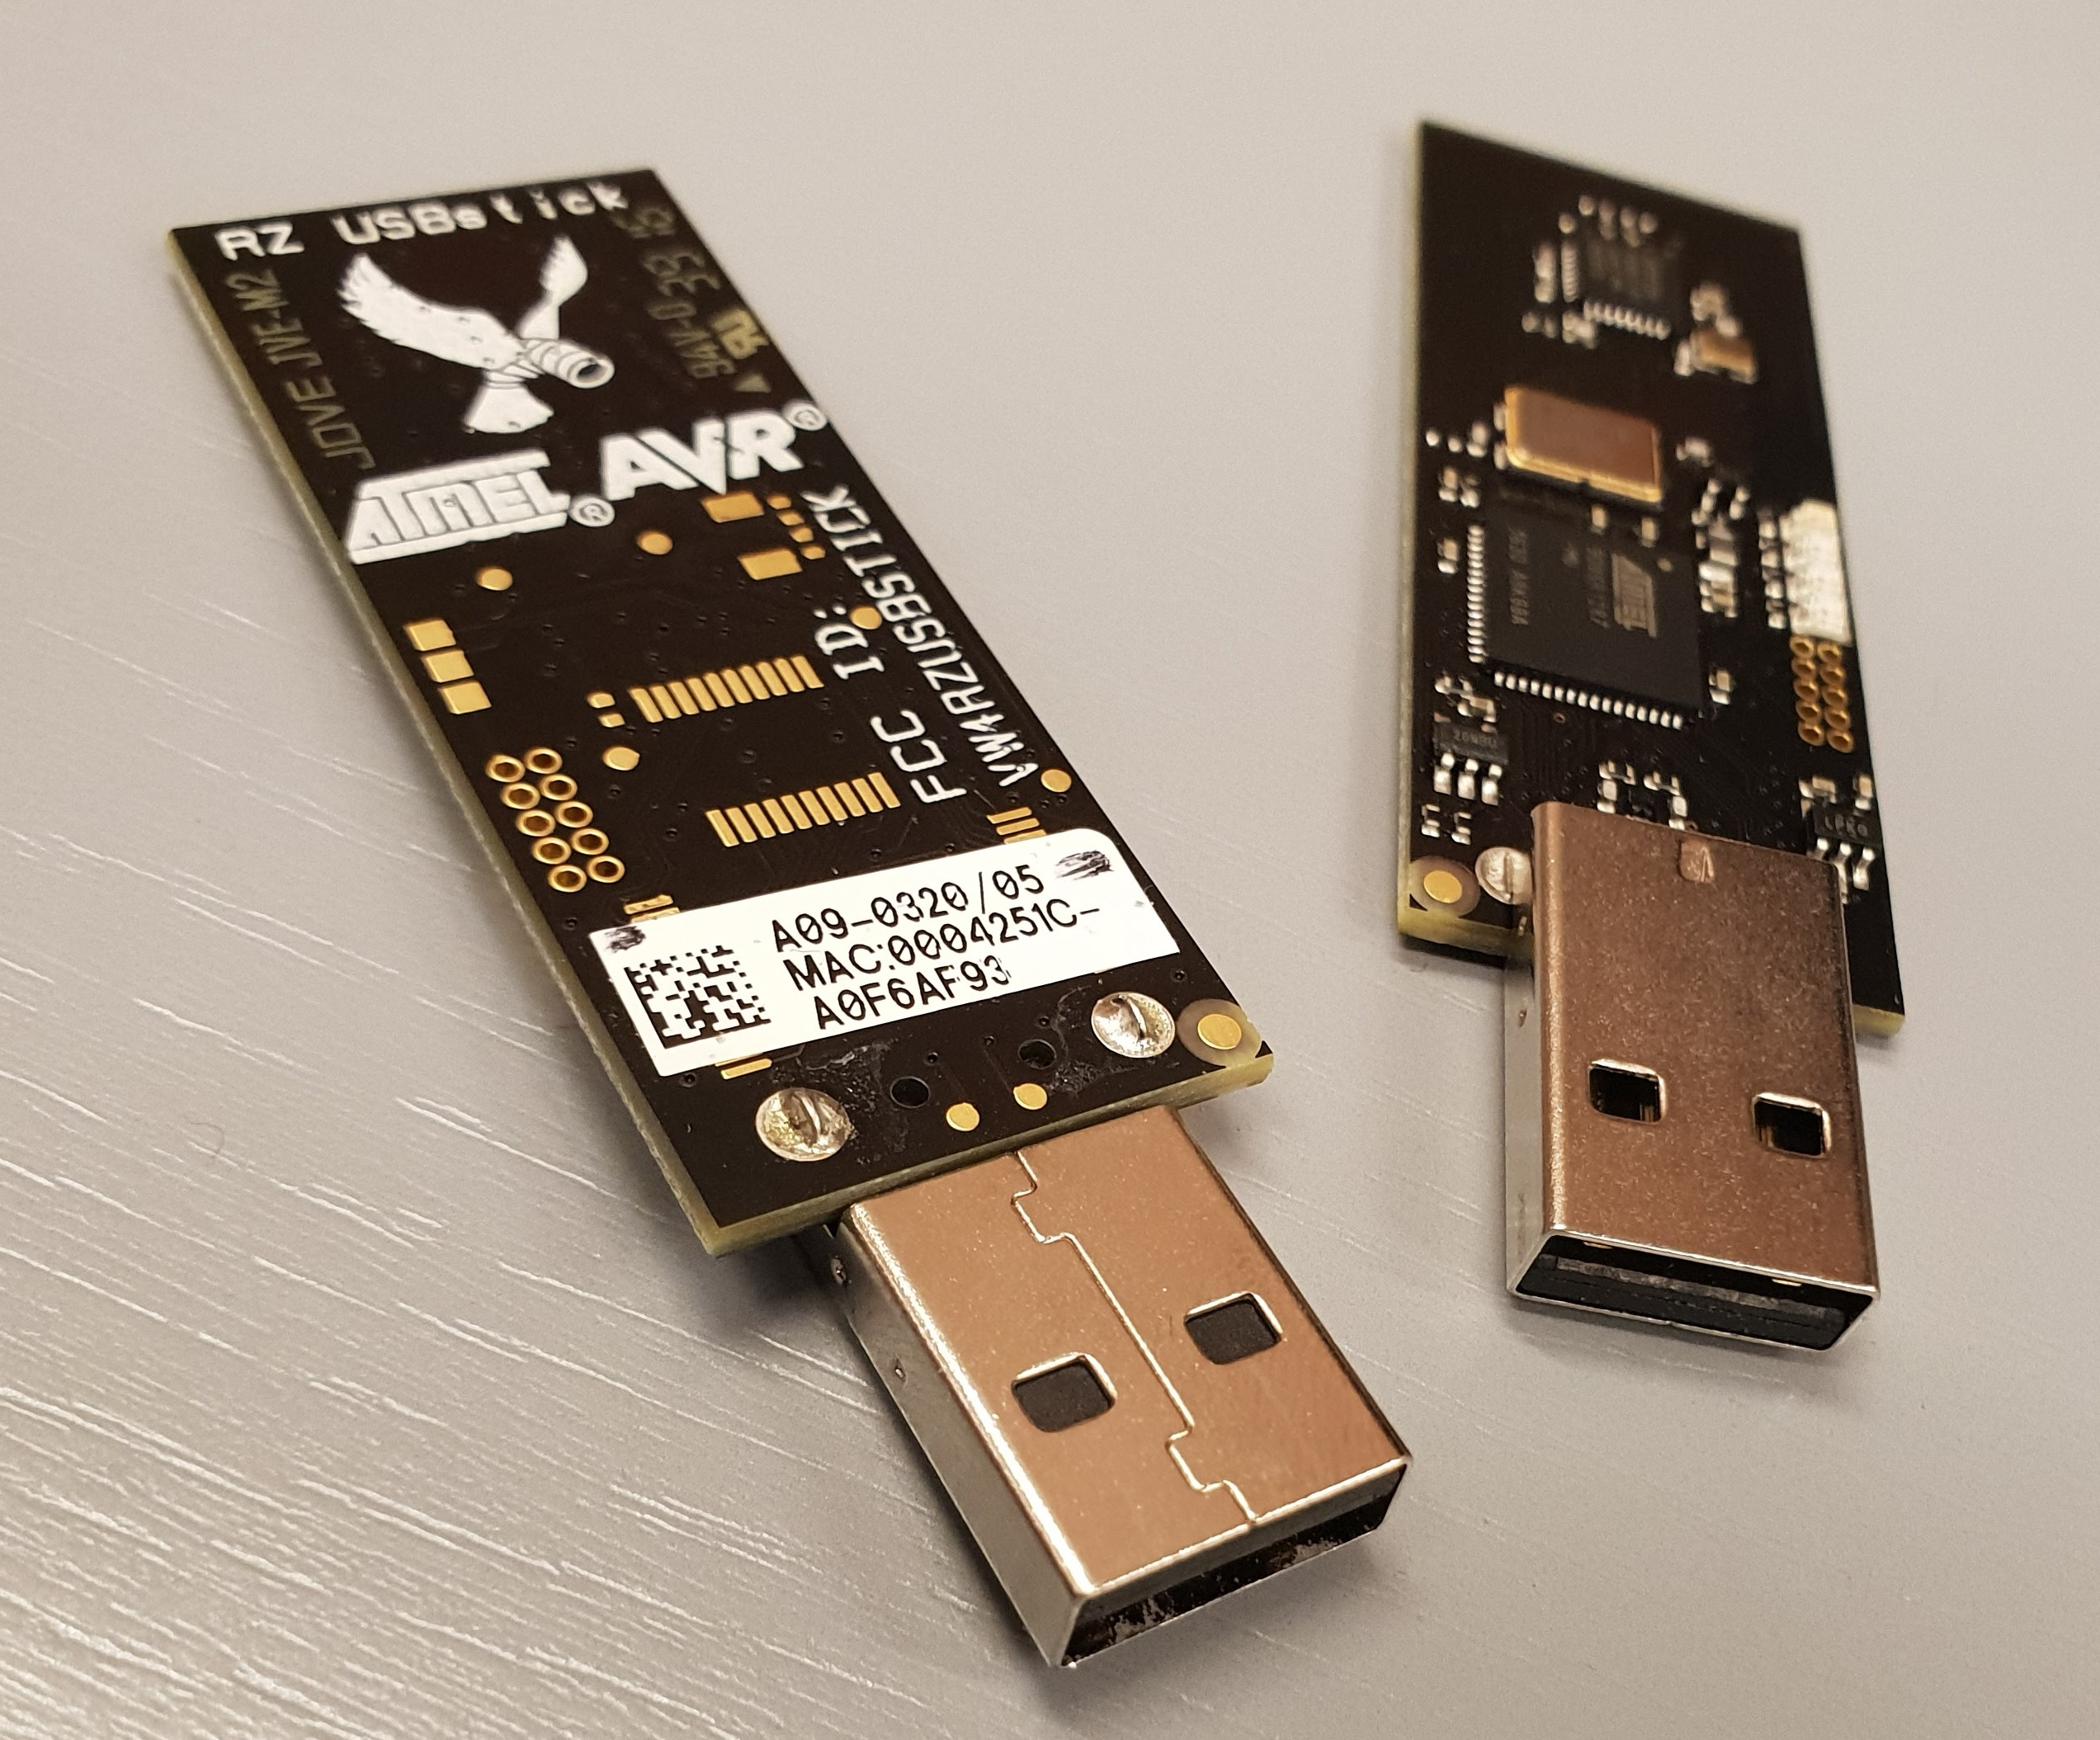
\includegraphics[width=0.6\textwidth]{usbstick}
  \caption{Atmel RZ RAVEN USB pinne til bruk i pen testing.}
\end{figure}

For å kunne teste verktøyet måtte en sette opp en maskin med Linux Operativsystem. Til dette valgte en først å bruke en Oracle VirtualBox vituell maskin med Kali. Kali er Linux distrubert Operativsystem\cite{kali} utviklet for penetrasjon testing som allerede inneholder allerede Killerbee og var derfor et naturlig valg. Etter en del testing viser det seg at VirtualBox har problemer med å gripe USB enheter over vertmaskinen. VMware workstation player har derimot ikke dette problemet og er hva vi anbefaler å bruke i lab. Den forhåndsinstallerte versjonen av Killerbee i Kali fungerte heller ikke og måtte lastes og installeres på nytt. På en ny Linux VM installeres Killerbee samt alle nødvendige avhengigheter med følgende i terminal:

\begin{verbatim}
# apt-get install python-gtk2 python-cairo python-usb python-crypto python-serial 
python-dev libgcrypt-dev
# sudo apt install mercurial
# hg clone https://bitbucket.org/secdev/scapy-com
# cd scapy-com/
# sudo python setup.py install
# cd ~
# sudo apt install git
# sudo git clone https://github.com/riverloopsec/killerbee.git
# cd killerbee/
# sudo python setup.py install
\end{verbatim}

Ett annet alternativ var å bruke en USB minnepenn med live Linux operativsystem. En valgte også her å bruke Ubuntu da det latet til å være god støtte for å kjøre operativ systemet live fra en USB minnepenn\cite{ubuntulive}. En forutsetning var å ha varig lagring, altså å kunne lagre data mellom hver gang operativsystemet bootes opp og dette er ikke noe som er lagt opp som standardinnstilling. Det er flere veiledninger med programmer som eksempelvis Lili\cite{lili} og Unetbootin\cite{unetbootin} for å opprette en live USB minnepenn med varig lagring. Dette gjøres ved å opprette casper-rw, en blokk med varig minne og lese/skrivetilganger. Ingen av programmene som installerer OS og oppretter casper-rw i ett fungerte for oss. Se vår fremgangsmetode i Appendix.


Atmel RZ RAVEN USB penn kommer i utgangspunktet ikke med nødvendig firmware ferdig installert med mindre en bestiller den fra spesialiserte nettsteder og da til en betydelig høyere pris. Siste firmware kan lastes ned fra github siden til utvikler \cite{riverloops} med instrukser på hvordan man flasher USB. Metoden vi valgte var ikke avhengig av ekstra hardware som On-Chip programmerer men var kun mulig med Windows 7 x86 da det ikke fungerer med 64 bit drivere. Universitet skaffet en Windows 7 x86 ISO fil som en brukte til å satte opp virtuell maskin i VMware workstation player. Begge USB pinnene ble så flashet med siste firmware ved bruk av Atmel AVR Wireless Services. Pennene kan nå benytte alle Killerbee verktøy. 

\begin{figure} [!ht]
	\centering
		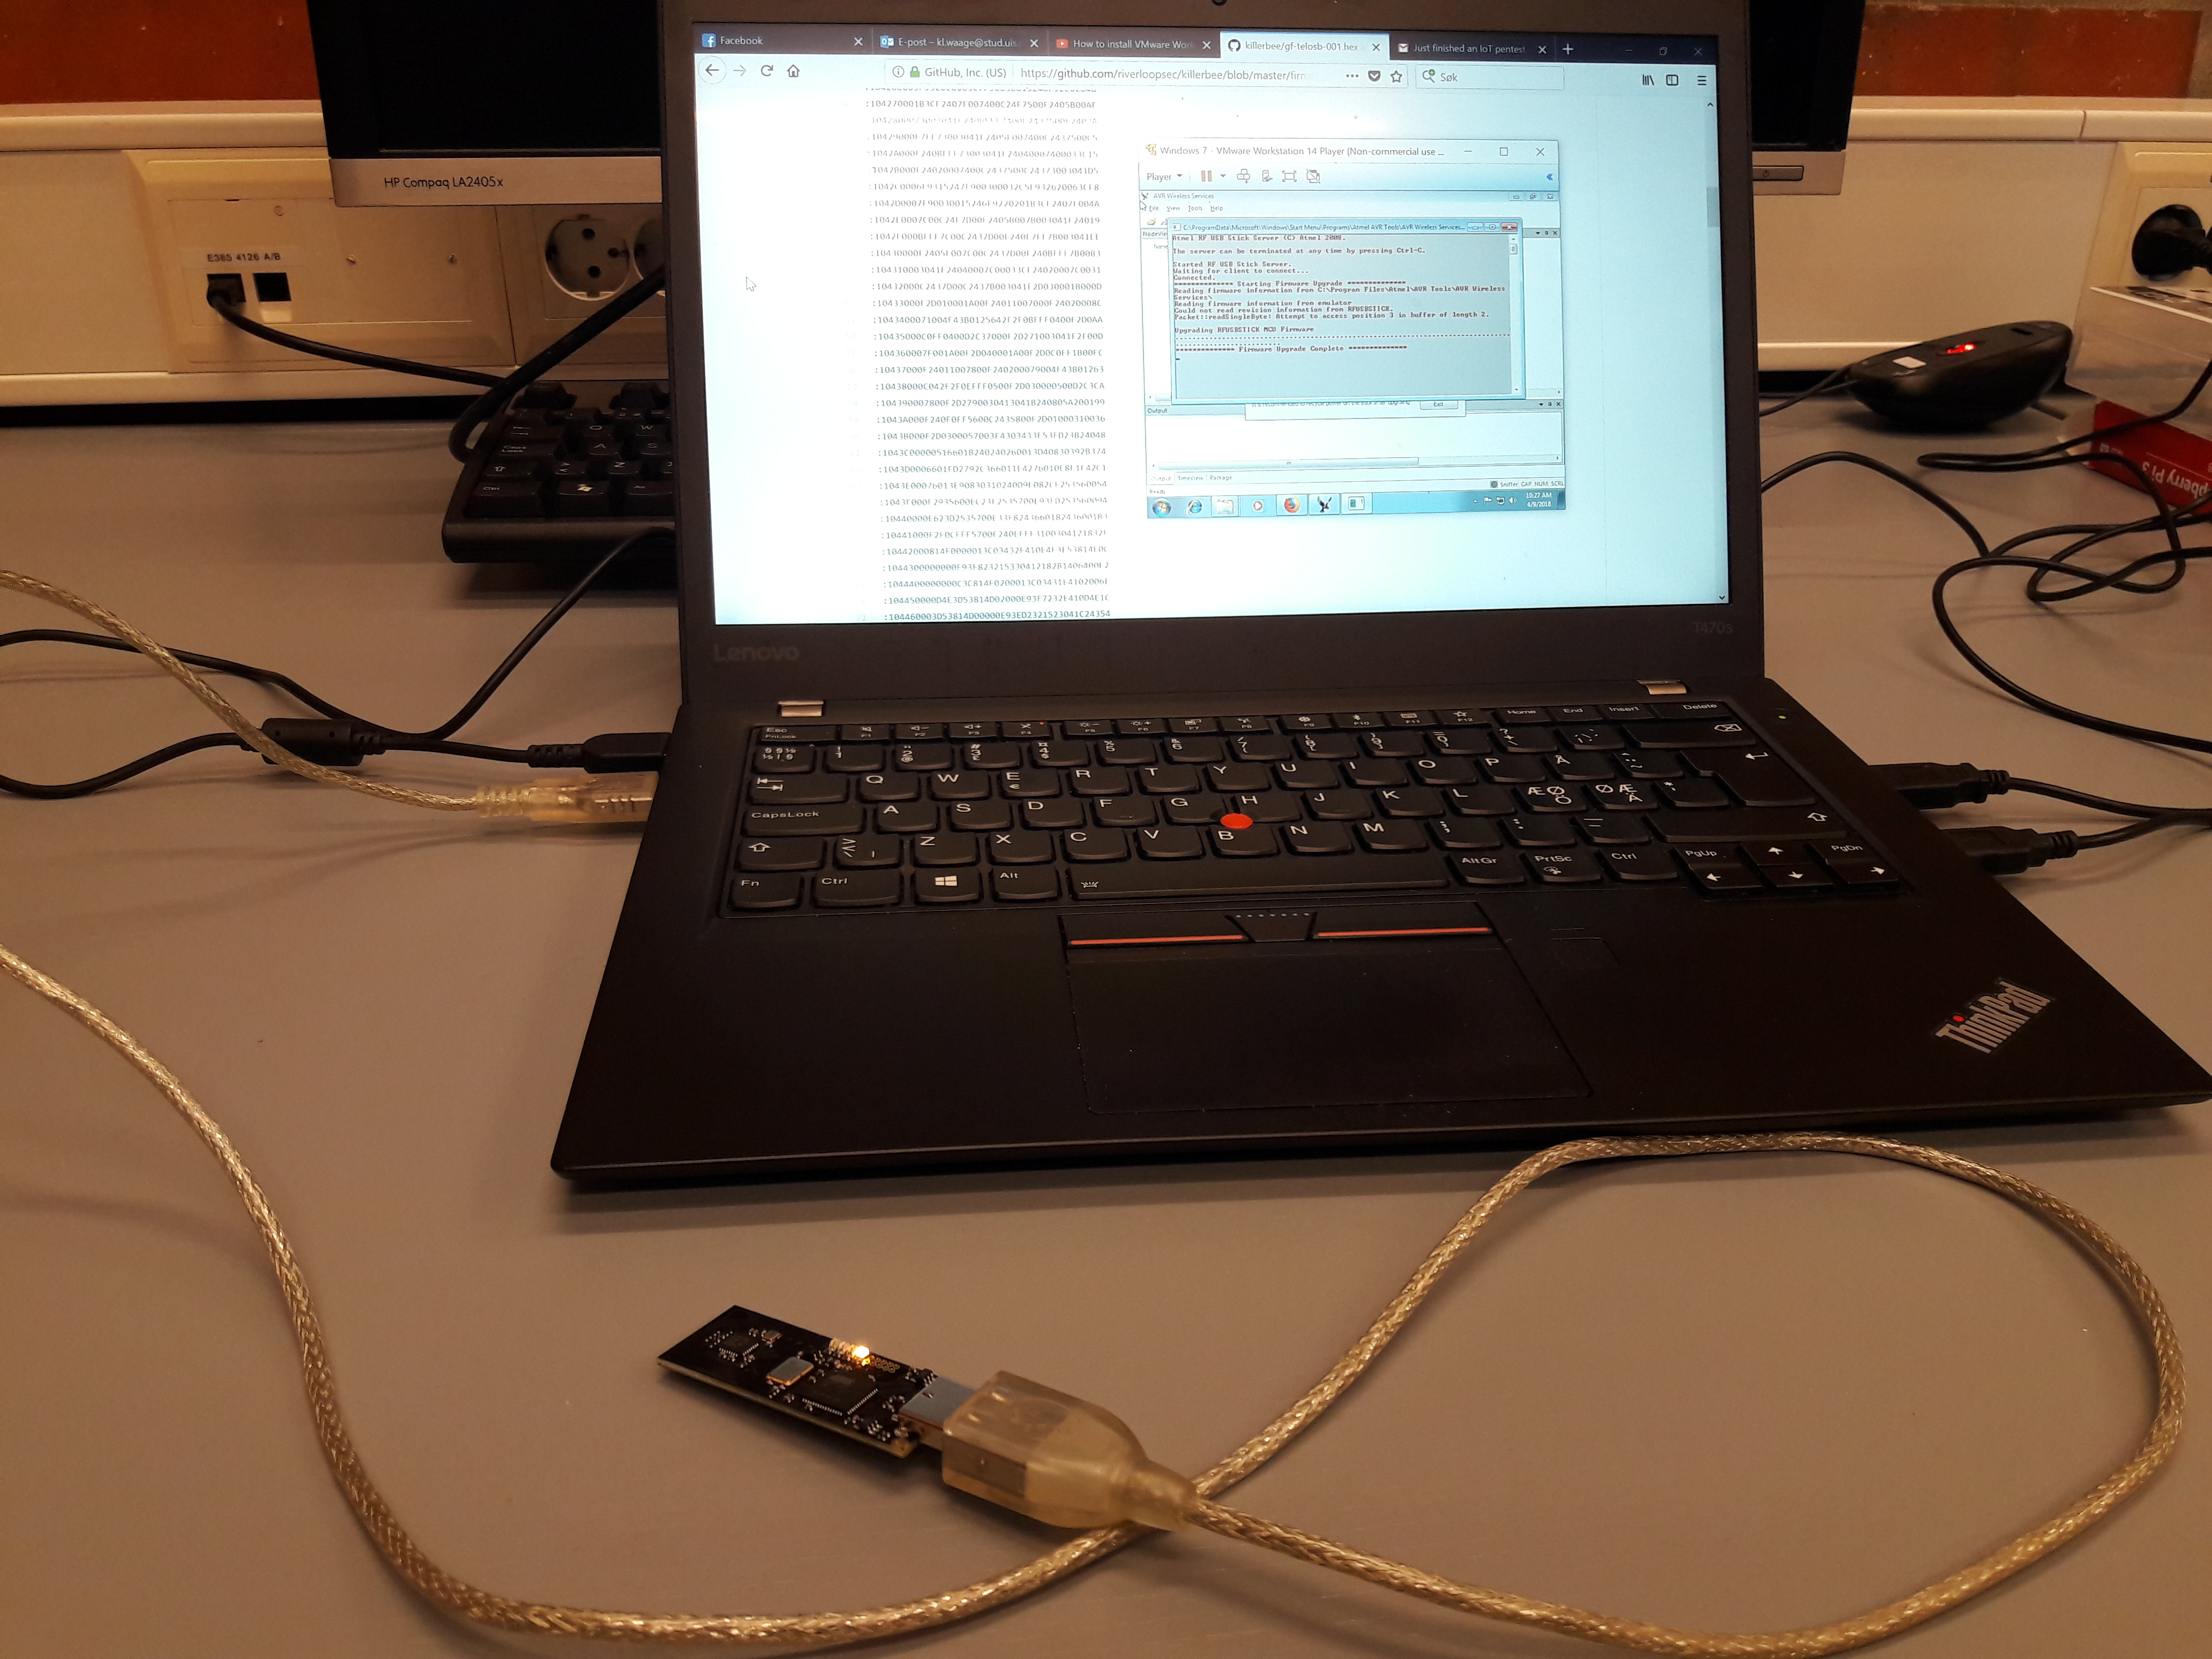
\includegraphics[width=0.85\linewidth]{flashefw} 
\caption{Flasher her den ene RZ RAVEN USB pennen med siste Killerbee firmware fra River Loops. Etter at ny firmware har hatt en vellykket installasjon vil lampen endres fra blå til oransje.}
\end{figure}



\subsection{LoRaWAN}
LoRaWAN er en trådløs protokoll for sending over lange avstander og lavt strømforbruk. Det er en protokoll som er tatt i bruk av Stavanger Smartby for å kunne motta informasjon fra mange forskjellige noder spredt ut over store avstander. Noder som sender data om luftkvalitet, vannstand, ledige parkeringsplasser, forbipasseringer i handlegater osv. Det som er ekstra gunstig er at disse nodene  ikke trenger å bytte batteri på opp til flere år. Med tanke på at denne teknologien skal brukes mer og mer i stavanger smartby, mente vi det var hensiktsmessig for studenter ved UiS å ha kjennskap til protokollen og kunne implementere den. 

\subsubsection{Dragino LoRa/GPS Hat for Raspberry Pi}
For å kunne implementere LoRaWAN på IoT laboratoriet så ble det bestemt at LoRa/GPS\textunderscore HAT for Raspberry Pi var det beste valget. Dette er en ekspansjon modul for Raspberry Pi som lar deg montere den og bruke Raspberry Pi som en billig LoRaWAN gateway løsning. 

\begin{figure} [!ht]
	\centering
		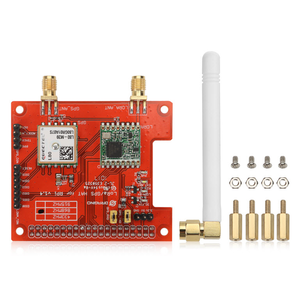
\includegraphics[width=0.5\linewidth]{loradraginohat} 
\caption{LoRaWAN Dragino modul for Raspberry Pi}
\end{figure}

Den har også en GPS modul. Modulen har en programmerbar bitrate opp til 300 kbps, har et link budsjett på 168 dB, og en innebygget temperatur og lavt batteri indikator. 

\subsubsection{Gateway}
For å sette RPi med LoRa/GPS\textunderscore HAT som en LoRaWAN gateway må man klone noen github repositories for å lag. For å sette denne opp som en DCPF må \\\url{https://github.com/bokse001/dual_chan_pkt_fwd} repositoriet klones. Etter dette klones så må man inn i konfigurasjonsfilen og endre om noen pin-assignments, og sette posisjonen til gatewayen. Når dette er gjort, så vil RPi-en med HAT-en kunne motta LoRa meldinger og være synlig på thethingsnetwork.org - den ledende LoRa-utvikler nettsiden.

\subsubsection{The Things Network}
The things Network er en nettside og et forum for LoRaWAN utviklere. Det er det ledende forumet for denne protokollen, og har over 38000 medlemmer som aktivt arbeider med å implementere LoRaWAN gateways og noder rundt omkring i verden. Når man har en LoRaWAN gateway kjørende, og koblet til The Things Network, så kan man se den på deres kart over aktive gateways. 
Man kan utforske dette kartet, og trykke seg inn på alle de forskjellige gatewayene for å få informasjon om plassering, hvilken type gateway det er, hvilken antenne som er i bruk, og dens adresse. 


\begin{figure} [!ht]
	\centering
		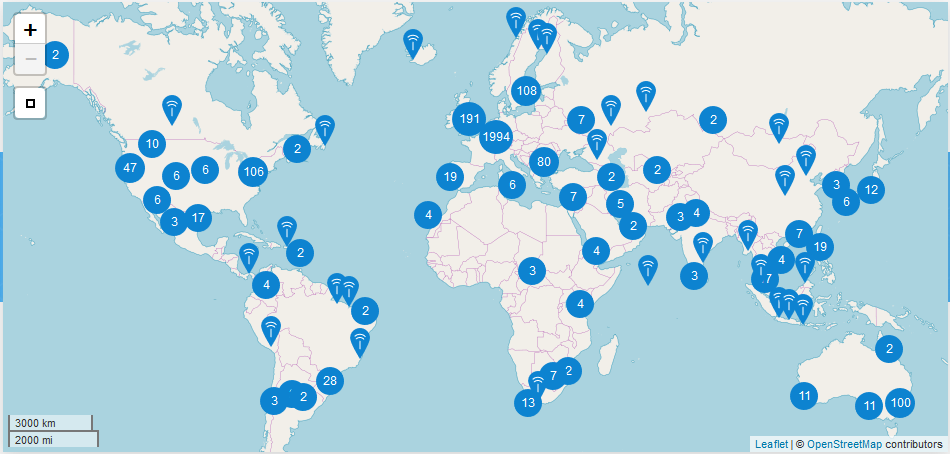
\includegraphics[width=0.75\linewidth]{TTNMap} 
\caption{The Things Network kart over LoRa noder}
\end{figure}

\subsubsection{Noder}
I løpet av dette prosjektet så har vi hatt mye fokus på forskjellige protokoller og teknologier. Vi har fått en LoRaWAN gateway opp og funksjonell, men en ting vi ikke fikk til i denne oppgaven var å få en funksjonell LoRaWAN node opp. Det ble testet en del forskjellige ting. Den mest lovende løsningen var å omprogrammere vår LoRa Dragino HAT om til en node. Dette viste seg å møte på en del problemer som ikke var ukjente for oss til dette punktet. Programvaren som ble lagt frem, og fremgangsmåten på å installere det var begge utdatert, og fungerte ikke på operativsystemet Debian Stretch, og var også utdatert i forhold til de nylige endringene som ble gjort på The Things Network nettsiden. 

Hadde vi hatt mer tid til å gjøre denne oppgaven så kunne nok denne LoRaWAN noden til slutt blitt funksjonell, men ettersom vi hadde mange andre ting som også trengte oppmerksomhet, så ble LoRaWAN noden nedprioritert. 

\subsubsection{Stavanger Smart By}
Når vi utarbeidet vårt løsningsfor IoT labben, var det viktig for oss å se på hvilke teknologier som blir brukt i Stavanger regionen. Den største drivkraften bak dette viste seg å være Stavanger Smart By, der det allerede har blitt implementert flere sensorer som tar inn bland annet CO2, luftkvalitet, støy og temperatur for så å sende data ved hjelp av LoRaWAN og WiFi. 

Stavanger Smart By er et prosjekt for å utarbeide et LoRaWAN nettverk for implementering av IoT, og for å gi byen WiFi. Nettet bruker LoRaWAN da dette er en strømbesparende teknologi som gir muligheten for å bruke sensorer med batteri som strømforsyning. Ved bruk av for eksempel Bluetooth vil det nemmlig være problematisk å bruke batterier da bluetooth bruker mer strøm en LoRaWAN. 

\subsection{Miljøovervåkning i E-472 Versjon 1}
Som en del av vårt bevis for at IoT labben virker, valgte vi å sette opp en miljøovervåkning i rack Antarktis i E-472. Her bruker vi en RPi med SenseHat modulen til å hente inn temperatur, luftfuktighet, lufttrykk og til å registrere om RPien har blitt flyttet. Det skrives også ut temperaturen på en 8x8 LED matrise på SenseHat modulen. Fargen på matrisen endres fra grønn til oransj dersom temperaturen stiger over 35 grader, og fra oransj til rød om den stiger over 45. Fargene er ment som alarmer, der oransj vil bety at man må passe på og rødt vil signalisere fare. Dersom temperaturen i skapet er over 45 grader vil dette somregel signalisere at noe er galt. All informasjonen er satt til å publiseres ut på Internett til en nettside. Ideen om dette har kommet fra Altibox, der dette er noe som brukes for å monitorere noderom. På nettsiden har vi også valgt å publisere data fra værforholdene i ommråde og et kart der lokasjonen på RPi er innlagt. Dette er for å illustrere hvordan dette vil bli brukt i industi, ikke bare på en lab. Målet med denne første versjonen av en miljøovervåkning har vært å lett kunne illustrere for personer med relativt lav forståelse for nettverk, programmering og sensorer hvordan prossesen går fra sensor og ut på internett. Denne ble også lagd med tanke på fremmvisning på åpen dag.

\begin{figure}
  \centering
      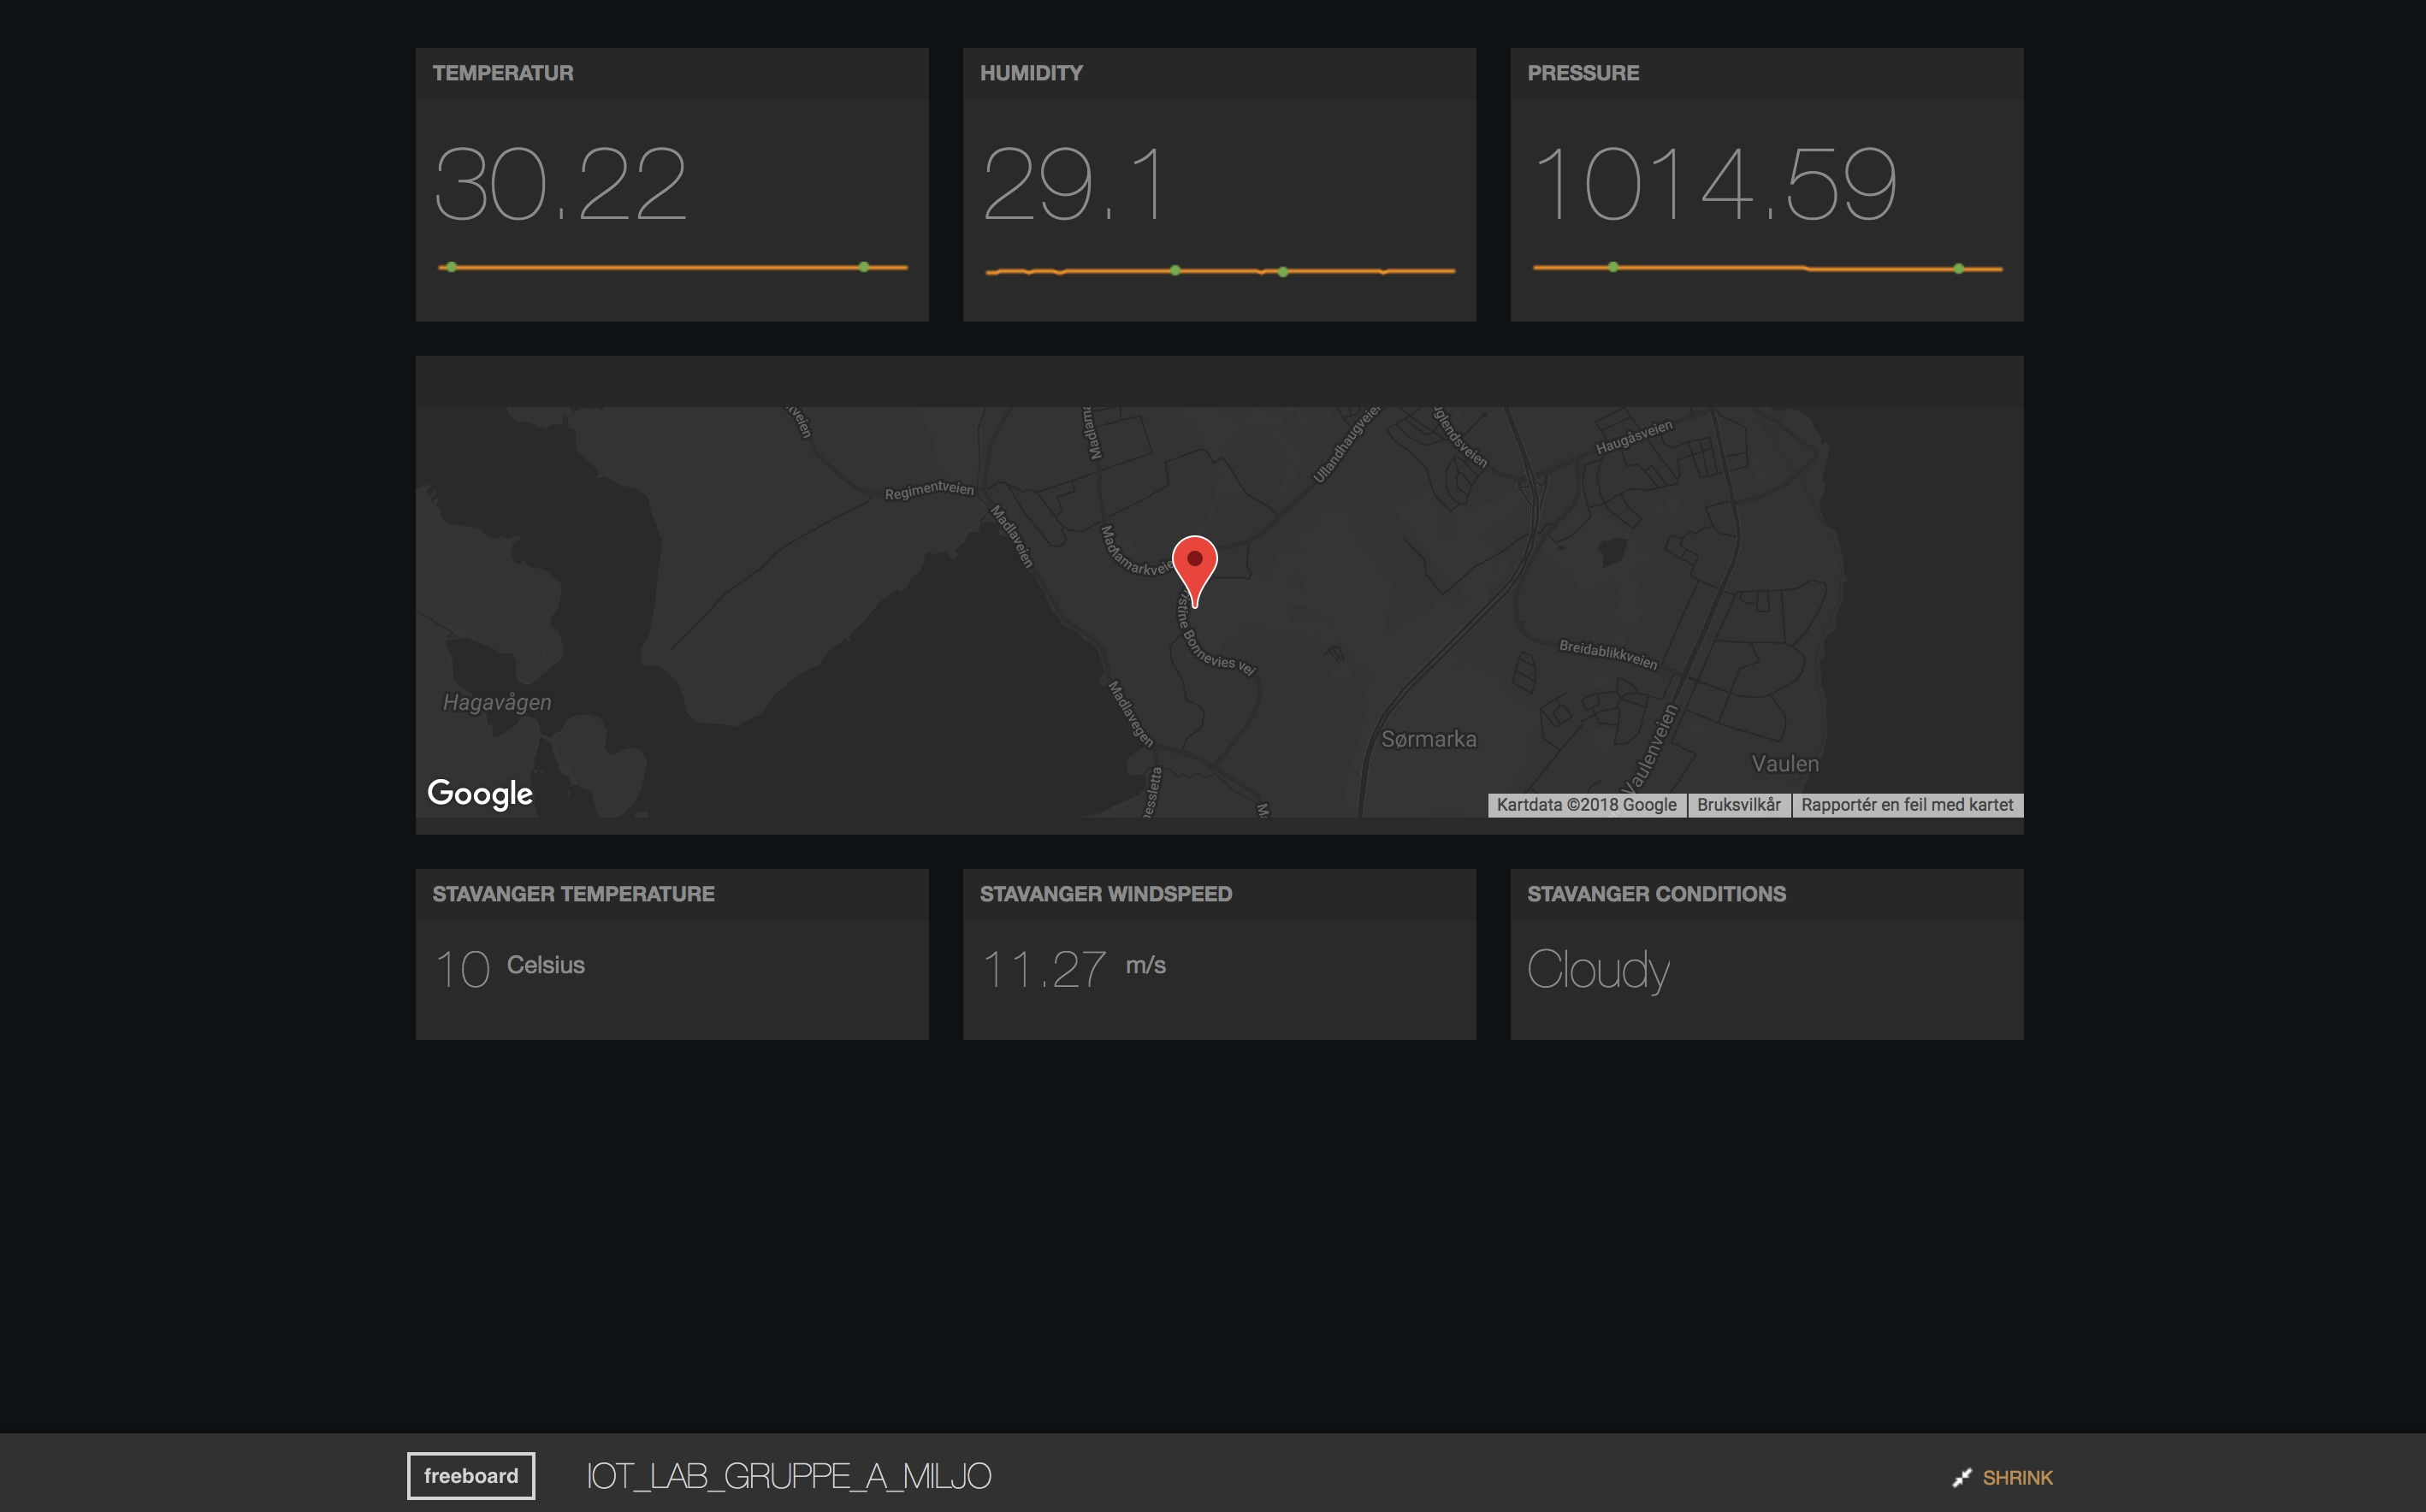
\includegraphics[width=0.9\textwidth]{freeboard}
  \caption{Freeboard.io layout med temperatur, luftfuktighet, lufttrykk, værforhold og lokasjon.}
\end{figure}

\subsubsection{Fysisk oppkobling}
Vi har valgt å koble RPi til en strømmforsyning over skapet merket Antarktis, dette er skapet hvor IoT routerene og switchene er plassert. Strømmkabelen er trukket gjennom toppen av skapet og koblet til RPien som er plassert midt i skapet. Vi har valgt denne strømmforsyningen for å kunne ta i bruk LED matrisen og for å kunne sende via WiFi. RPien har blitt tildelt IP-adressen 192.168.1.35, og er koblet til det dedikerte IoT aksesspunktet vårt, kallt KomtekIoTgruppeA. Så her har vi altså valgt å bruke WiFi som protokoll for sending av data, dette er fordi vi har en stor nok strømmforsyning tilgjengelig. Å bruke WiFi gir større båndbredde og derfor raskere sending av data, vi har tatt i bruk 2,4 GHz frekvensen.

RPi har festen en SenseHat modul som er tilkoblet alle GPIO pinnene, på denne finner vi alle sensorene. Her har vi temperatur, luftfuktighet, lufttrykk, joystick og gyroskop som måler bevegelse i X, Y og Z rettning. Vi har valgt å ikke hente inn data fra joystic, da dette ikke er interessant for en miljøovervåkning.

\begin{figure}
  \centering
      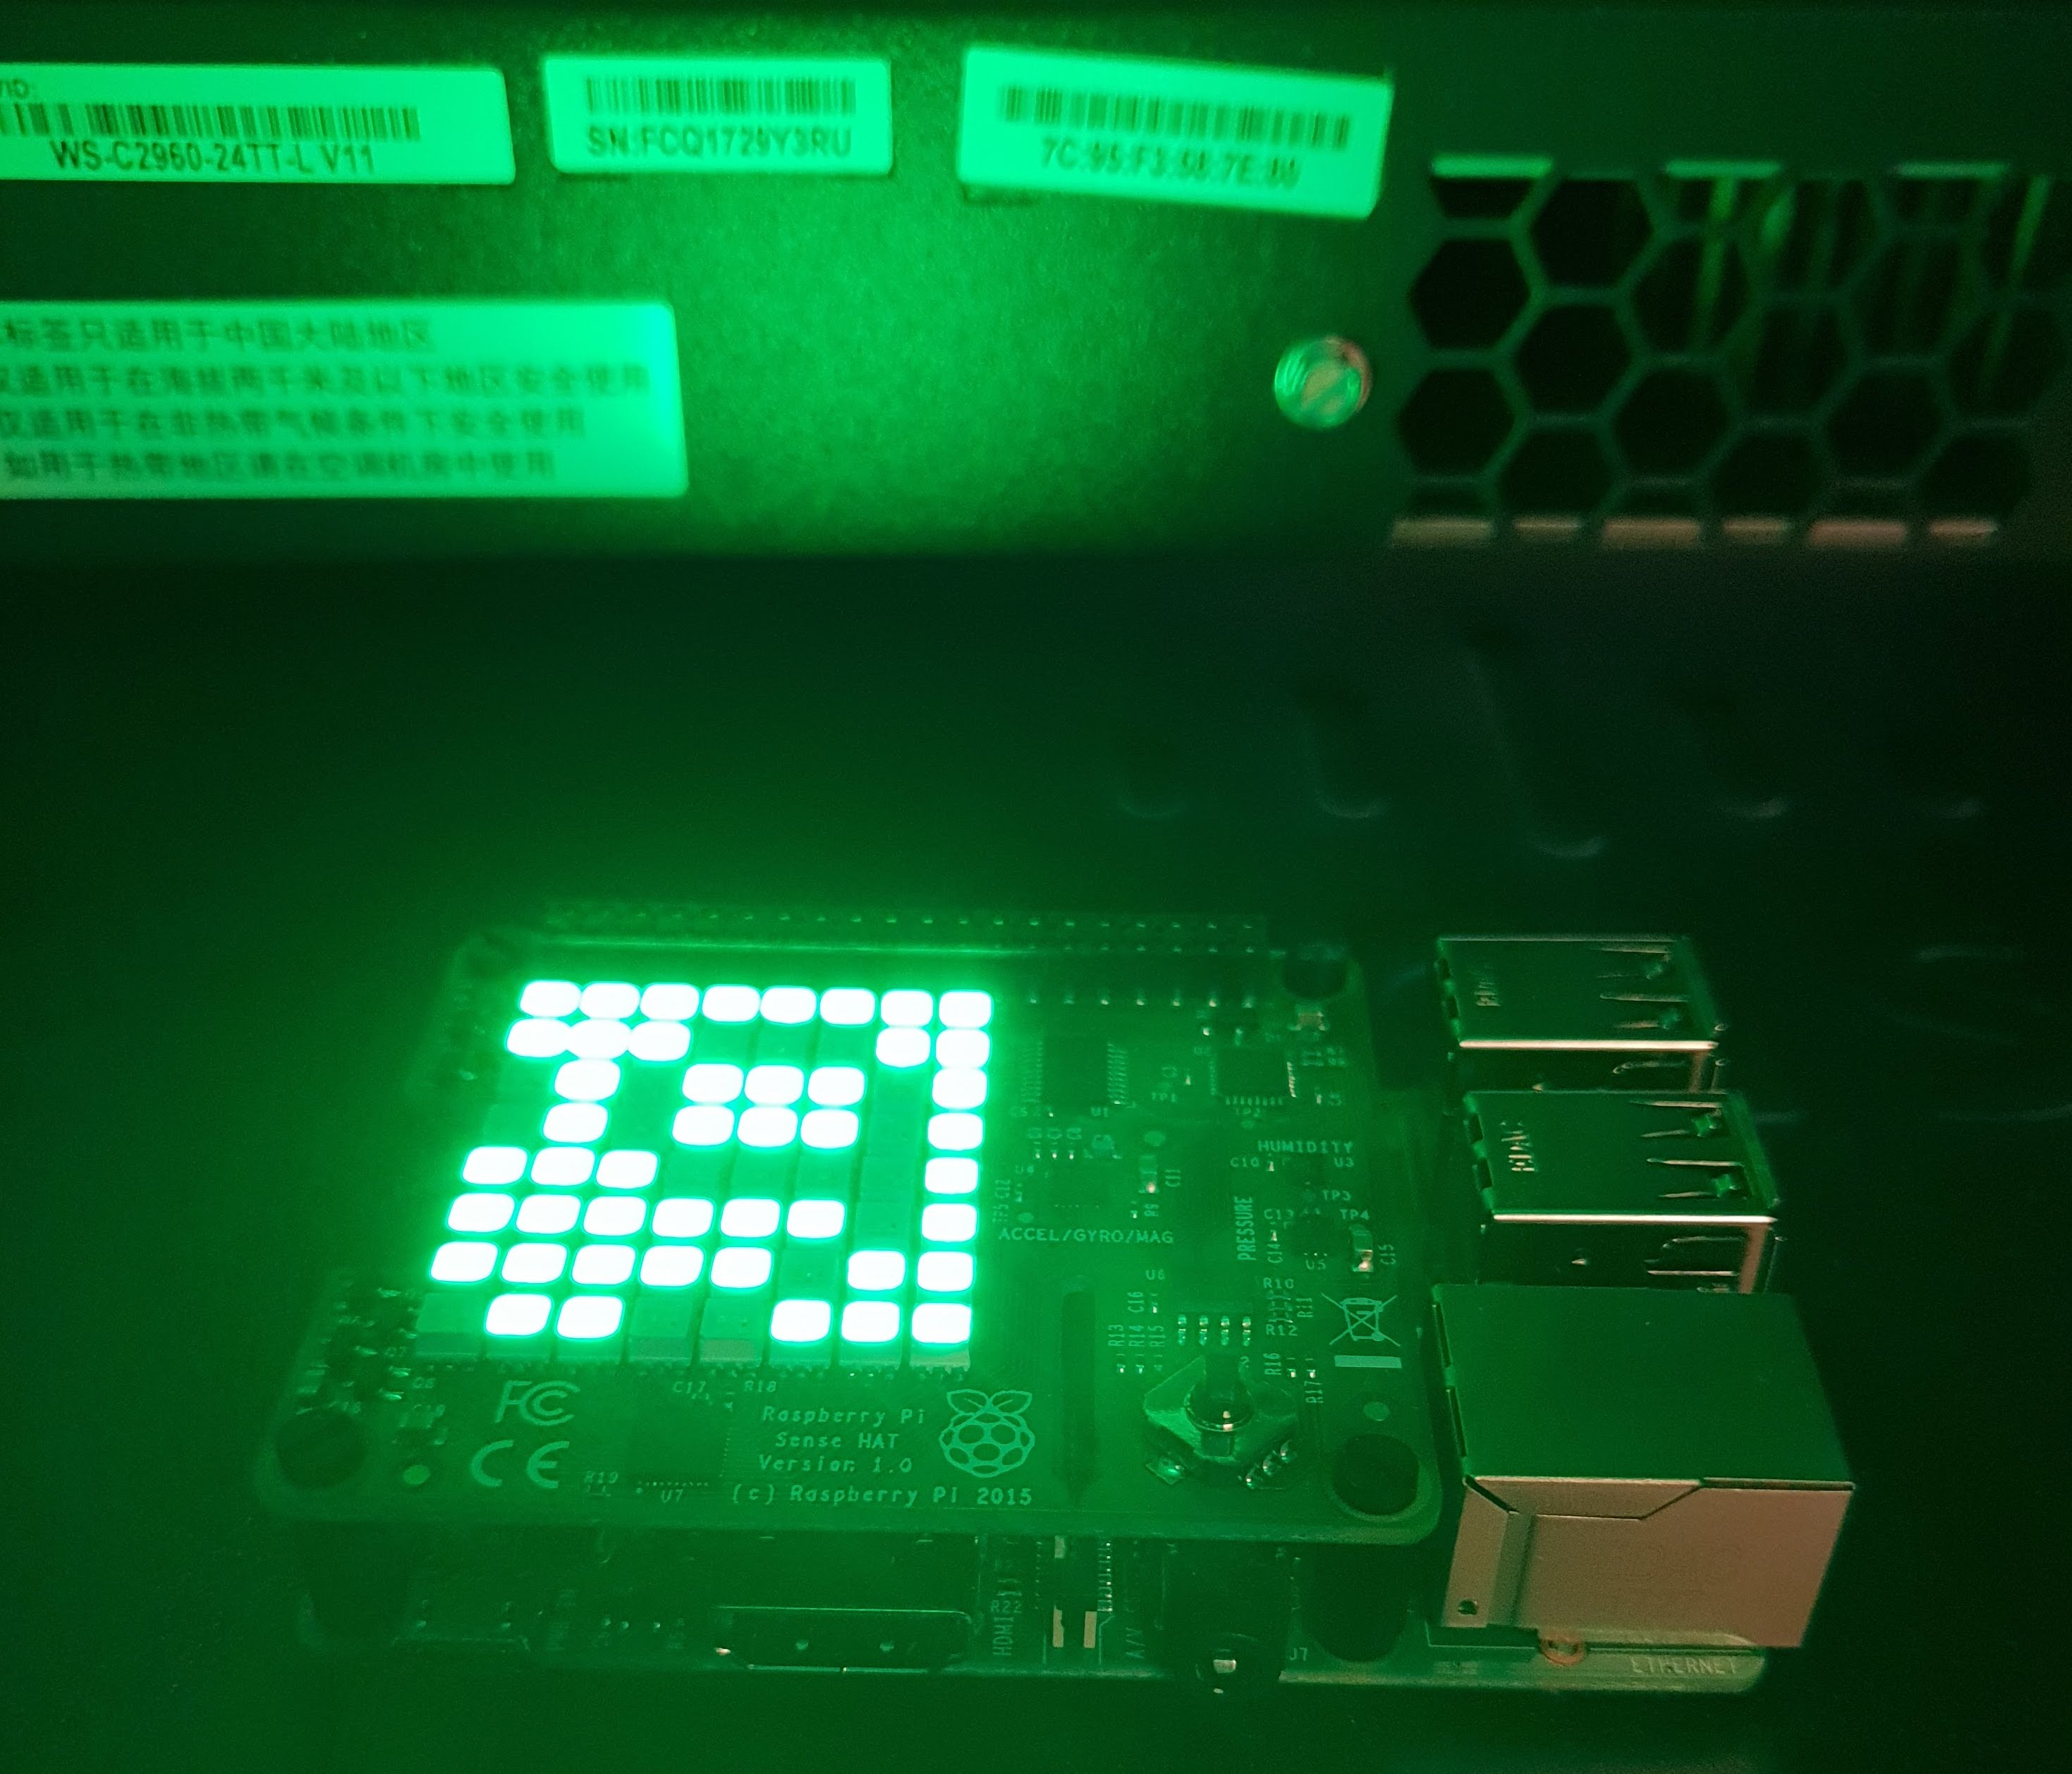
\includegraphics[width=0.9\textwidth]{rpimiljo1}
  \caption{Fysisk oppkobling av Miljøovervåkning}
\end{figure}

\subsubsection{Publisering av data}
Data fra miljøovervåkningen blir publisert til web applikasjonen Freeboard, et verktøy lagd med tanke på IoT prosjekter. Plattformen har allerede en nettside, så det har ikke vært behov for å designe vår egen nettside. Da dette er et enkelt bevis på hvor lett man kan sende sensordata ut på nettet og monitorere. For å publisere data ut har vi valgt å hente inn sensor data gjennom python bibliotekene som er spesiallagd for RPi SenseHat. For så å sende data ut ved Python Requests biblioteket. Begge bibliotekene krever særegen installasjon på RPi, så dette var første steg i programmerings prosessen. Under finner vi koden som publiserer til web applikasjonen dweet.io, en applikasjon lagd for nettopp denne typen testing.

\begin{lstlisting}[language=Python, caption=Python Dweet.io publisering]
from sense_hat import SenseHat
import time
import requests

sense = SenseHat()

red = (255, 0, 0)
green = (0, 255, 0)
orange = (255, 215, 0)
txt = (0, 0, 0)

def readData():

	temp = sense.get_temperature()
        temp = round(temp, 2)
        temp_str = str(temp)
        print("Temperature in C: ", temp)

        humidity = sense.get_humidity()
        humidity = round(humidity, 2)
        humidity_str = str(humidity)
        print("Humidity: " , humidity)

        pressure = sense.get_pressure()
        pressure = round(pressure, 2)
        pressure_str = str(pressure)
        print("Pressure: ", pressure)
        print("Str: ", pressure_str)

        if temp > 36:
                sense.show_message(str(temp) + "C! Major alarm", text_colour=txt, back_colour=red)
        elif temp >= 33 and temp <= 36:
                sense.show_message(str(temp) + "C! Minor alarm", text_colour=txt, back_colour=orange)
        else:
                sense.show_message(str(temp) + "C", text_colour=txt, back_colour=green)

        url = "https://dweet.io/dweet/for/iot_lab_gruppe_a_miljo?" + "Temperatur=" + temp_str + "&Humidity=" + humidity_str + "&Pressure=" + pressure_str

        r = requests.post(url)

while True:
        readData()
        time.sleep(10)
        
 \end{lstlisting}


\subsubsection{Åpen dag}
Som en del av Universitetet i Stavangers åpen dag har denne miljøovervåkningen blitt brukt brukt som en del av Data og Elektro sin stand. Denne miljøovervåkningen demonstrerer veien fra sensor gjennom hardware til et nettverk og ut til internett, allt programmert av studenter på en enkel og forståelig måte. Dette er med på å inspirere fremmtidige studenter, og å konkretisere hva Data og Elektrofag kan brukes til.

\subsection{Miljøovervåkning i E-472 Versjon 2}
For videre testing av teknologier innen IoT ble det aktuellt å ta i bruk ZigBee nettverket og Node- RED som en addisjon til miljøovervåkning i E-472. I denne versjonen har Node-RED blitt benyttet til innhenting av sensordata både fra RPi SenseHat og fra xBee Development Boards. Data blir behandlet i en JavaScript funksjon for så å bli sendt videre til et Node-RED Dashboard som grafer data. I motsettning til Freeboard.io som er tilgjengelig fra internett, er Node-RED Dashboard helt lokalt, og kun synlig for andre maskiner på nettverket. Dette er praktisk med tanke på nye reguleringer rundt sikkerhet og behandling av data fra tingenes internett. 

\begin{figure}[!ht]
  \centering
      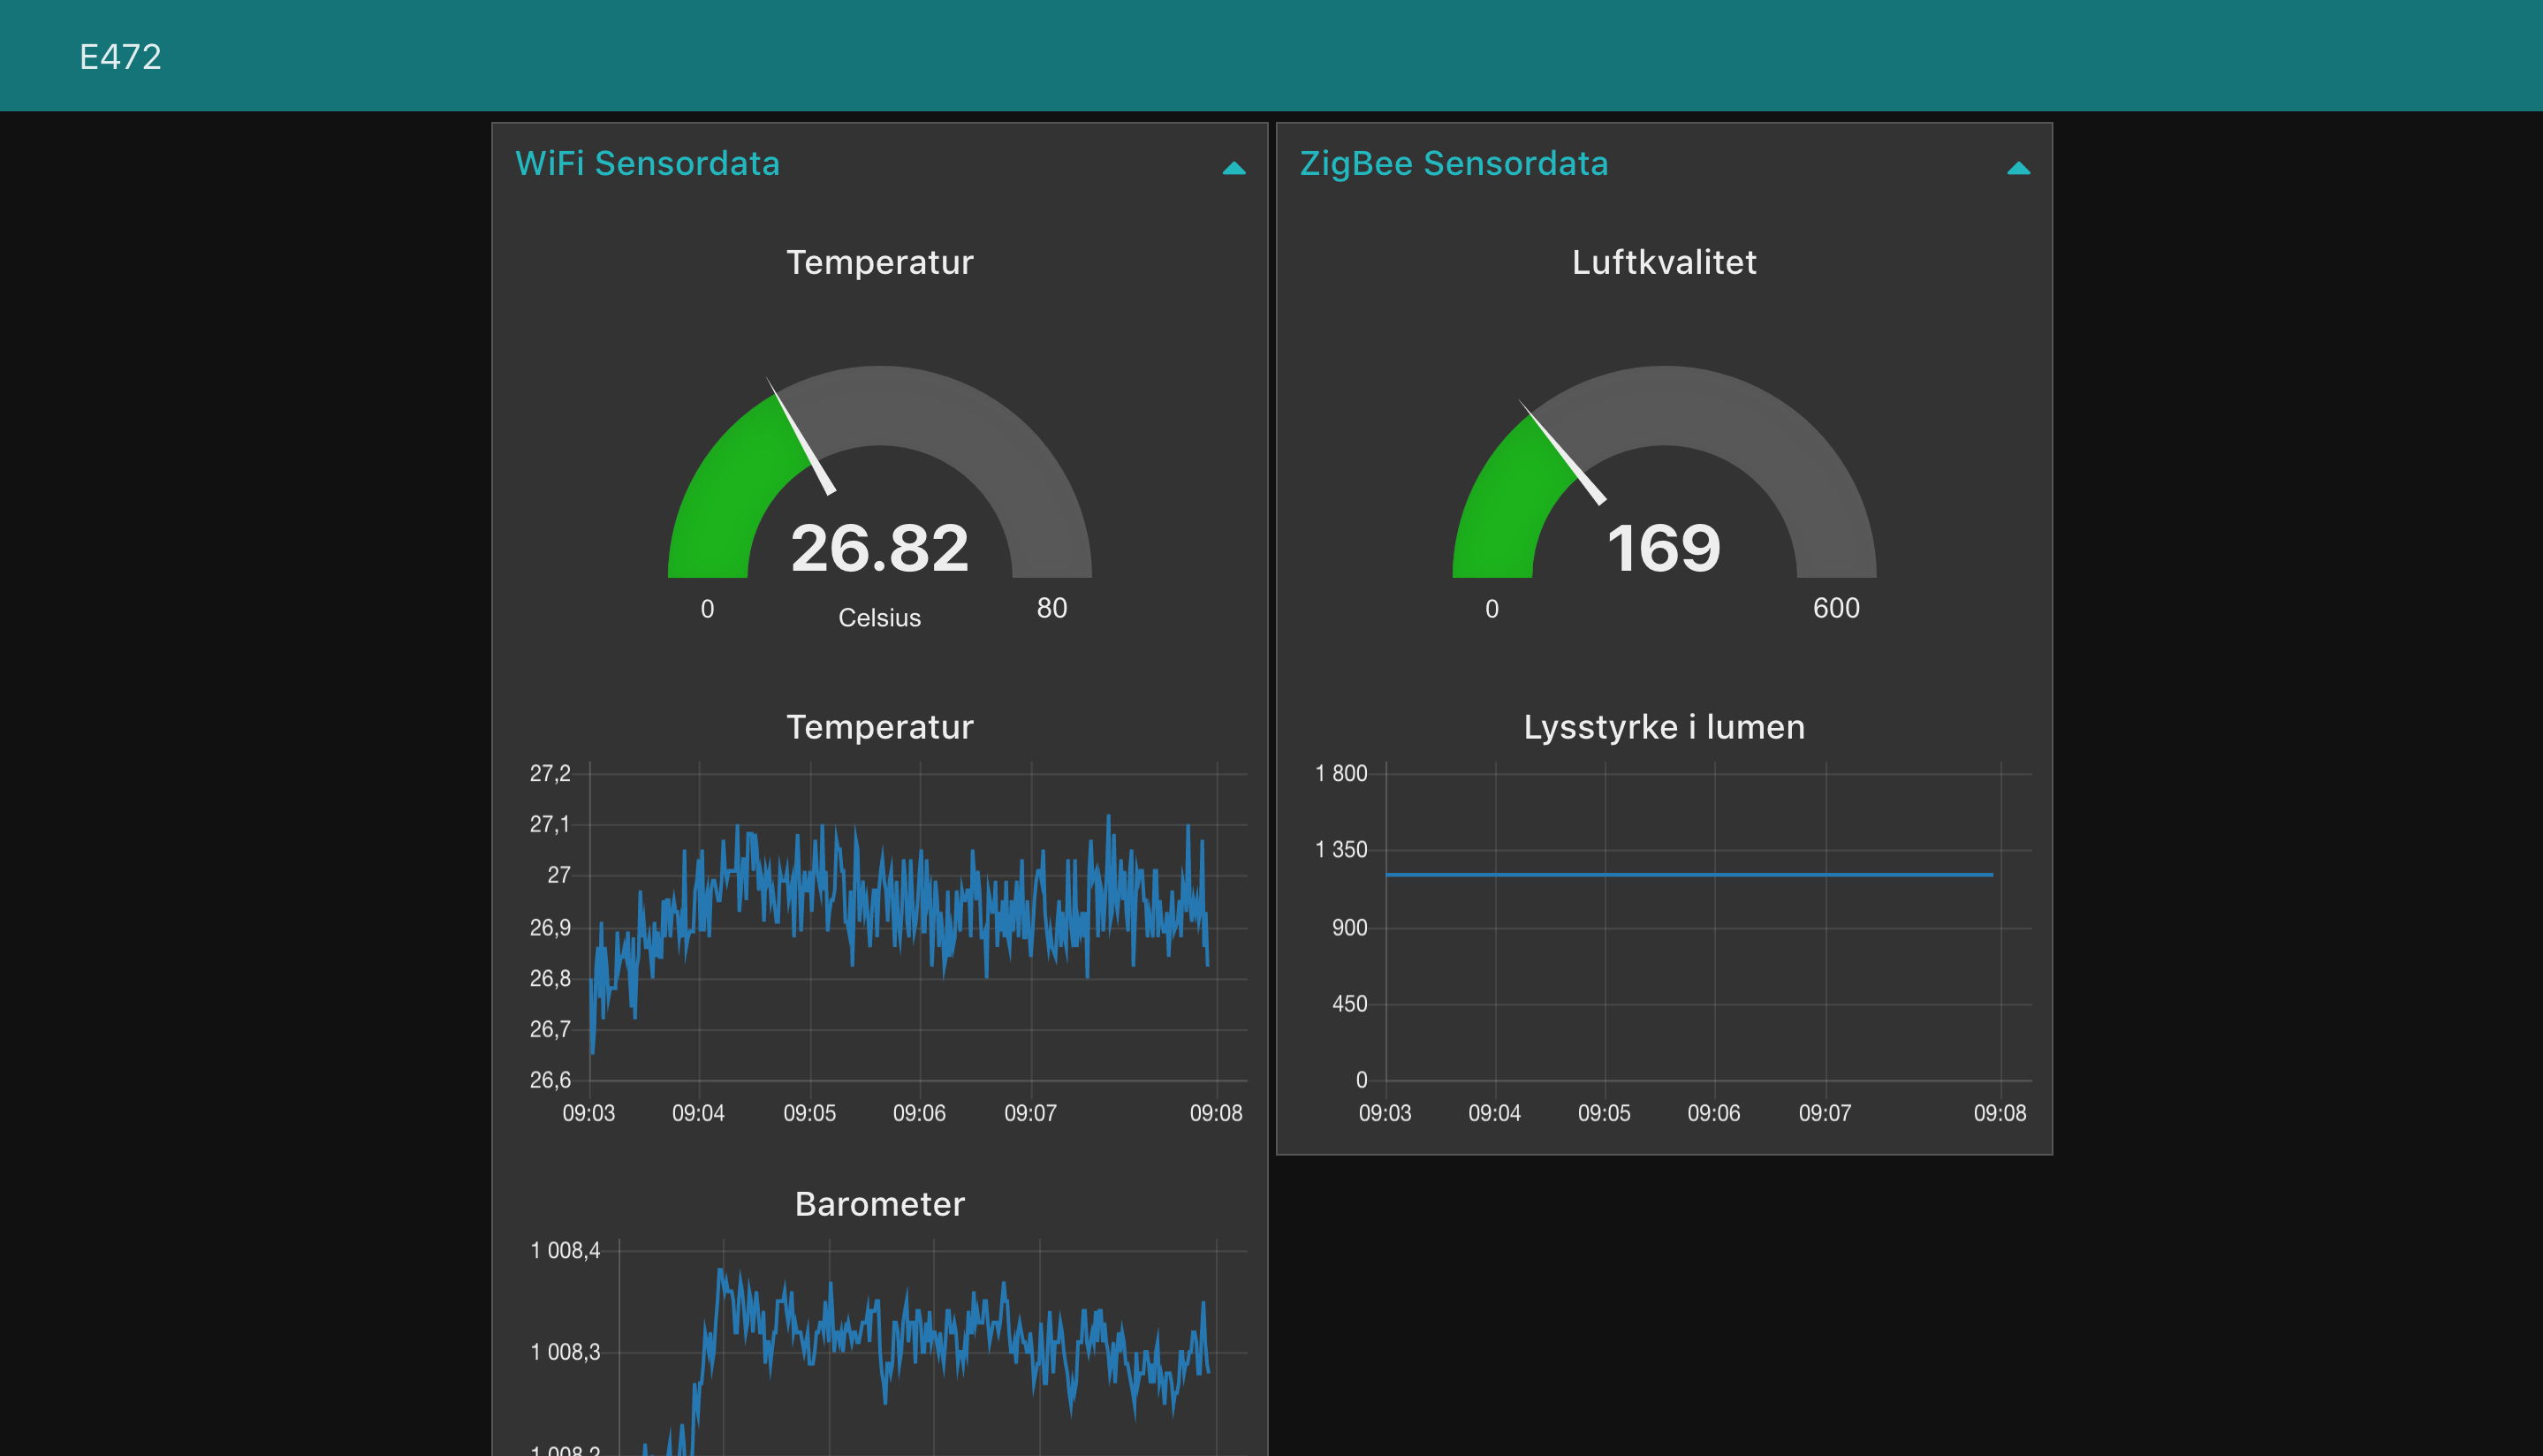
\includegraphics[width=0.9\textwidth]{iotdash}
  \caption{Miljøovervåkning Versjon 2 Dashboard}
\end{figure}

\subsubsection{Fysisk tilkobling}

Raspberry Pi er plassert i Antarktis skapet hvor den blir forsynt med strøm og henter temperatur, luftfuktighet og trykk en montert Sense Hat. ZigBee nettverkets koordinator noder er også tilkoblet RPi sin USB0 port hvor det sendes data og kortet får strøm til å drive ZigBee nettverket. Koordinatoren i ZigBee nettverket ruter trafikk og mottar sensor data fra en annen ZigBee node hvor en luftkvalitetssensor og en lyssensor er tilkoblet. Den er plassert ved studentassistentens datamaskin, det er enda ikke klart hva som vil være beste plassering for en optimal lesning av rommets luftkvalitet. ZigBee sensor noden får strøm fra en mikro USB kabel tilkoblet et strømuttak i veggen. Det vil være mulig å drive denne med batteri, men dette vil være unødvendig da det er flere lett tilgjengelige strømmuttak i E472. Det er mulig å vise frem miljøovervåkningen på en skjerm ved studentassistentes port ved å tilkoble en RPi eller en hvilken som helst annen datamaskin og åpne miljøovervåkningen i en nettleser.

\subsubsection{Innhenting av sensordata i Node-RED}

Under innhenting av sensordata brukes designerte noder for Sense Hat og for xBee, nodene er lagd av Node-RED utviklere og konfigureres gjennom det grafiske grensesnittet til å motta sensordata og sende det videre til en funksjon for bearbeiding. For innhenting av data fra RPi Sense Hat trengs ingen klargjøring eller konfigurasjon, her henter Node-RED data fra GPIO pinnene Sense Hat er tilkoblet. For henting av data fra ZigBee nettverkets koordinator kreves en seriell tilkobling, som nevnt tidligere er koordinatoren tilkoblet USB0 på RPi. Her sendes data gjennom og inn i Node-RED ved bruk av en xBee rx node. Denne må konfigureres med MAC adressen til koordinatoren i nettverket, ellers vil resten av konfigurasjonen være klargjort i vårt tilfelle. Om det i fremtiden vil bli benyttet annet utstyr, kan det skape behov for endring av overføringshastighet gjennom USB porten.

\begin{figure}[!ht]
  \centering
      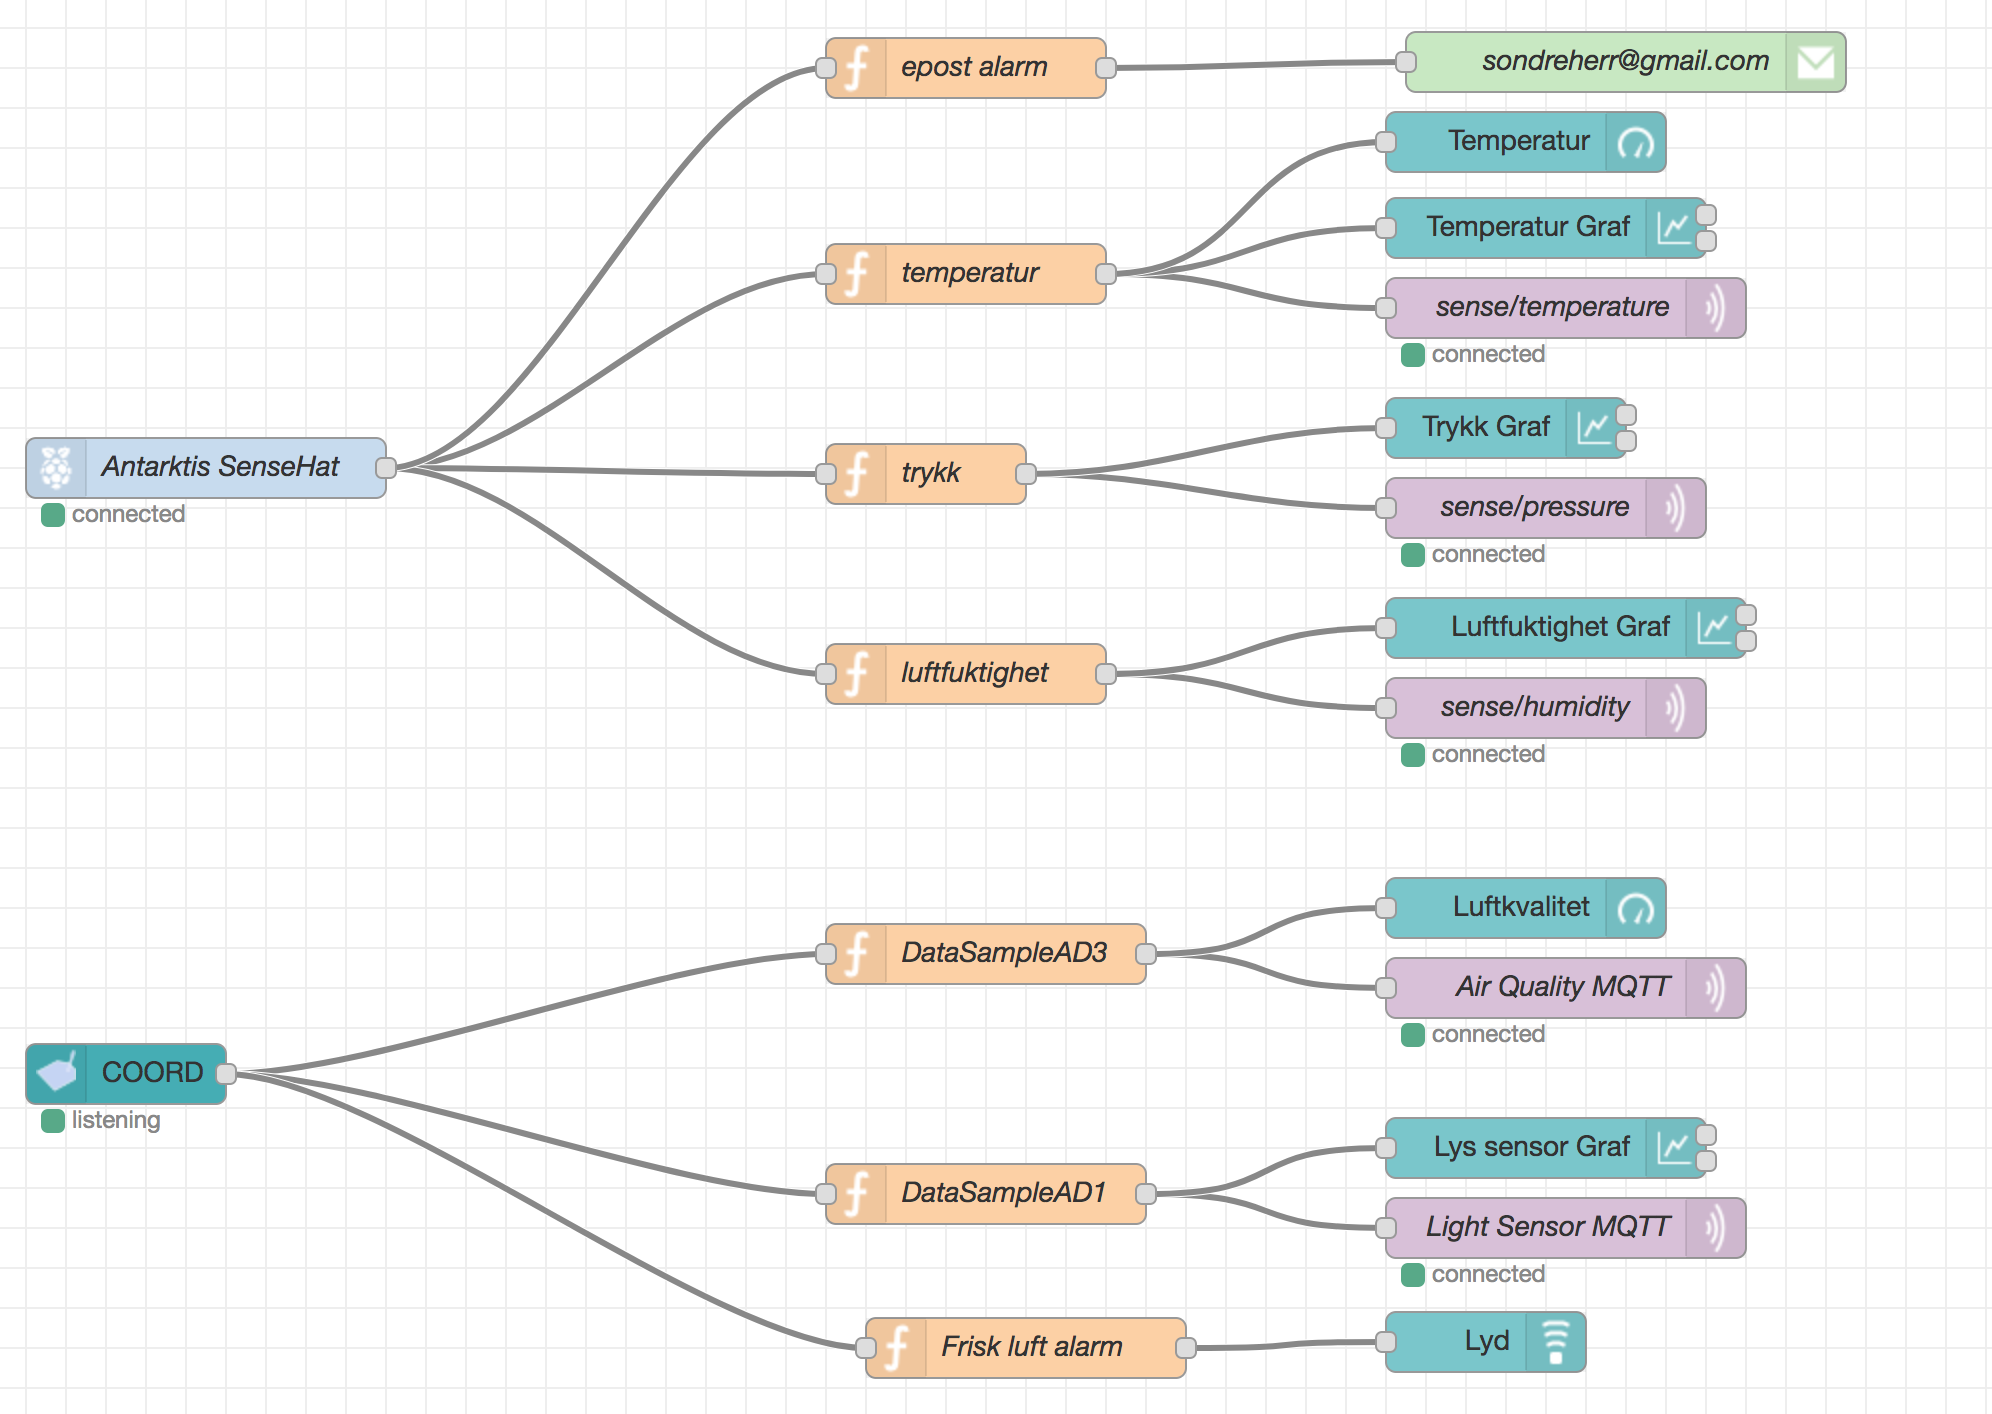
\includegraphics[width=0.9\textwidth]{Dashboard}
  \caption{Node-RED flow for Miljøovervåkning Versjon 2}
\end{figure}


\subsubsection{Konfigurasjon av ZigBee nettverket}
Konfigurering av ZigBee nettverket blir gjort gjennom verktøyet XCTU, et program laget for konfigurering av ZigBee noder. Første prioritet i bygging av et ZigBee nettverk er å konfigurere koordinator noden, dette er noden som styrer nettverket. Dersom ingen koordinator er klargjort vil ikke nettverket kunne opprettes da det ikke er noe som starter det opp eller tillater andre noder å tilknytte seg nettverket. Dette blir beskrevet i nærmere detalj i seksjonen om adressering i ZigBee, en fullstendig instruksjon på hvordan å konfigurere opp Et ZigBee nettverk med xBee Development Boards er lagt i Appendix. 

\begin{table}
\centering
\caption{Konfigurasjon av xBee Moduler for innhenting av analoge sensordata}
\label{xBeeKonfigurasjon}
\begin{tabular}{|l|l|l|l|}
\hline
	\textbf{Parameter} 				& \textbf{xBeeA}  					& \textbf{xBeeB}			\\ \hline
	
	\textbf{ID} 					& 1337  						& 1337			\\ \hline
	
	\textbf{JV} 					&  -							& Enabled			\\ \hline
	
	\textbf{CE} 					&Enabled 					&  -					\\ \hline
	
	\textbf{DH} 					&  -							&  0					\\ \hline
	
	\textbf{DL}					&  -							&  0					\\ \hline

	\textbf{NI} 					&  KOORDINATOR		& SENSOR		\\ \hline

	\textbf{AP} 					&  API enabled			&  API enabled	\\ \hline

	\textbf{SP} 					&  14F						&  1F4				\\ \hline

	\textbf{SM} 					&  -							& -					\\ \hline
	
	\textbf{D0} 					&  -							&  ADC				\\ \hline

	\textbf{D3} 					&  -							&  ADC				\\ \hline

	\textbf{IR} 					&  -						&  1388					\\ \hline
\end{tabular}
\end{table}


\subsubsection{Bearbeiding av data og publisering til Node-RED Dashboard}

Etter data er hentet inn i Node-RED trengs bearbeiding, grunnen til dette er at data som hentes inn er all data fra ZigBee nettverket og ikke avrundede verdier fra Sense Hat. Dette gjøres ved bruk av JavaScript funksjons noder som kobles til noden som henter data fra sensoren. Data som har blitt hentet inn i vår miljøovervåkning er lysstyrke og luftkvalitet fra ZigBee. Som data hentet fra WiFi har vi brukt Sense Hat for henting av temperatur, luftfuktighet og lufttrykk. 

\begin{lstlisting}[language=Java, caption=Funksjon for innhenting av temperatur data fra RPi Sense Hat]
var inn = msg.payload;
msg.payload = inn.temperature;
return msg;
\end{lstlisting}

\subsubsection{MQTT publisering av data}
Som en del av denne løsningen er det tilkoblet MQTT noder, deres funksjon er å sende ut data ved hjelp av MQTT protokollen til det lokale IoT nettverket som tilhører labben. Det vil kunne hentes inn av alle andre enheter på nettverket, og brukes til å lage grafer, monitorere temperatur og så videre. MQTT data som sendes blir sendt fra Raspberry Pi, som fungerer som både server og megler. Her genereres strømmer av alle sensor data innhentet i lab, fritt tilgjengelig for alle på nettverket. Sendingene er beskyttet av det laveste nivået av sikkerhet, brukernavn og passord, data blir med andre ord ikke kryptert. Dette gjør sending raskere, og mer strømbesparende. Dette er det beste alternativet for sending av ikke-sensitive data på et lukket nettverk.
\linebreak 
\begin{figure}[!ht]
  \centering
      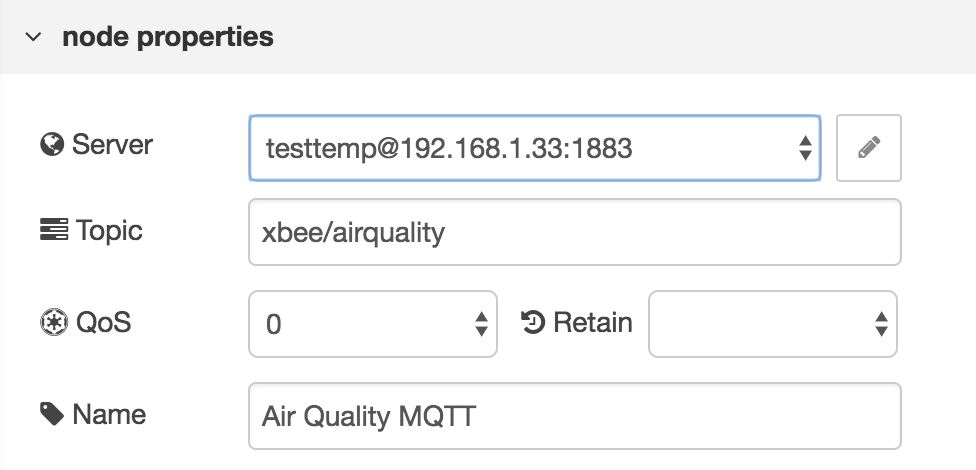
\includegraphics[width=0.5\textwidth]{xbeemqttkonfig}
  \caption{Node parametere for sending av MQTT}
\end{figure}

MQTT nodene er tilkoblet funksjons noder som har hentet ut data, på denne måten blir det kun videresendt data som tilhører den designerte MQTT strømmen. Når data når MQTT noden blir det videresendt fra klienten kalt “testtemp” som igjen er koblet til Raspberry Pi som fungerer som en vert/host. Denne finnes på IP-adressen 192.168.1.33, og porten som tas i bruk er 1883. Port 1883 er porten som er designer for usikker sending, som nevnt tidligere er strømmene beskyttet av enkelt passord. Keep-alive timer er satt til 60 sekunder for en sesjon. QoS er satt til nivå 0, dette er det laveste nivået. Grunnen til dette er at det ikke er farlig å oppleve litt pakketap og duplikater i denne situasjonen, her er fokuset på å ha en så direkte strøm av sensordata som mulig. 

MQTT oppsettet er lagret i Node-RED på denne måten vil studenter lettere kunne teste sending av data uten unødvendig mye konfigurering. Om en student ønsker vil han/hun kunne koble opp node, og velge testtemp@192.168.1.33:1883 malen for så å kun måtte spesifisere navn på strømmen studenten ønsker å sende gjennom. Det også så klart mulig å sette opp en egen klient i Node-RED om det skulle være ønskelig. Det er også mulig å motta MQTT data gjennom Node-RED ved å benytte en MQTT mottaker node, dette har vi ikket tatt i bruk da det for øyeblikket ikke er behov. Det er laget en mal for mottakelse av MQTT strømmer dersom studenter ønsker å benytte seg av dette i fremtiden.

\begin{figure}[!ht]
  \centering
      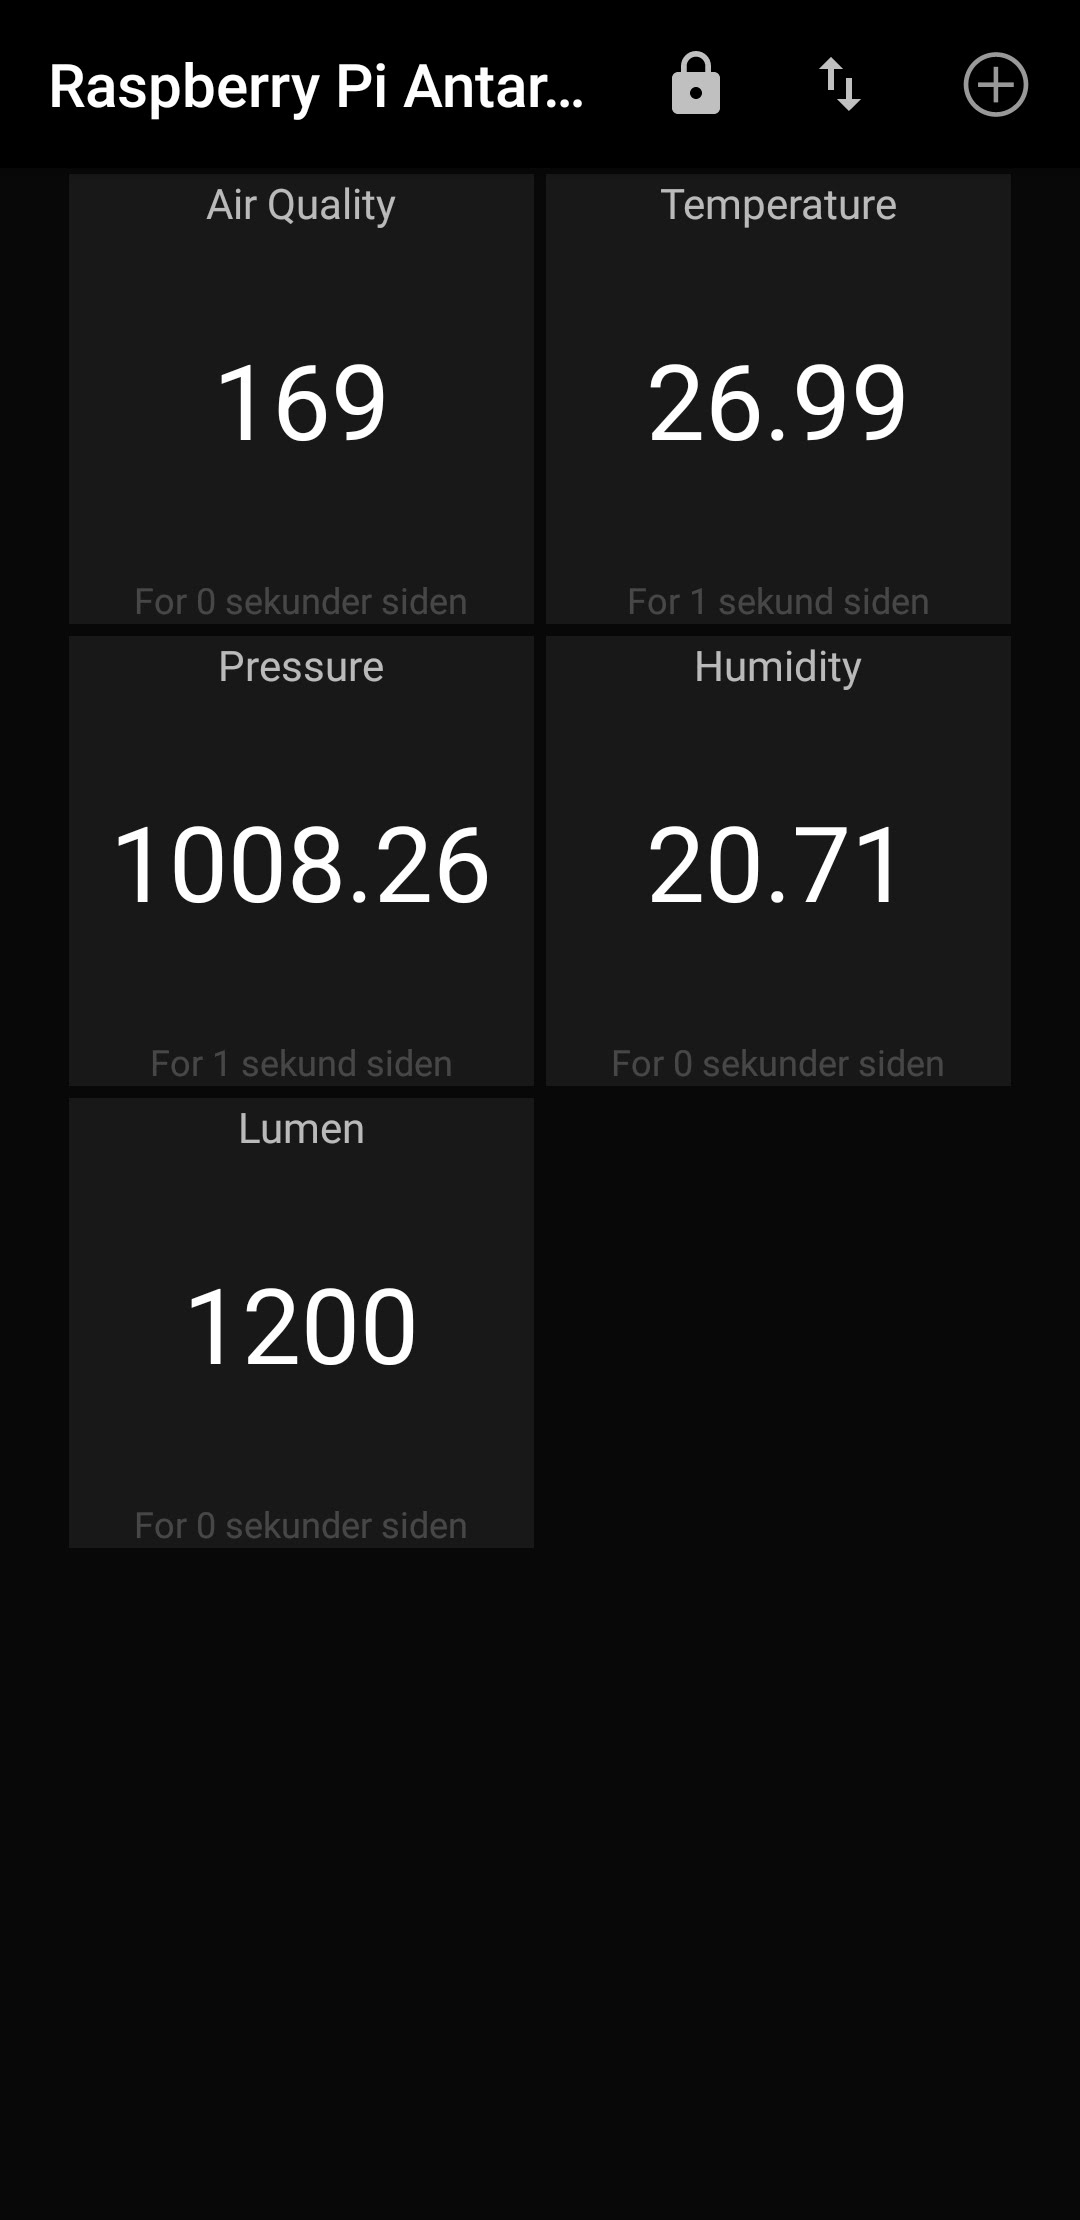
\includegraphics[width=0.3\textwidth]{mqttmobil}
  \caption{Eksempel på monitorering av sensordata sendt via MQTT til en Android app}
\end{figure}


\begin{table}[]
	\centering
	\caption{Oversikt over MQTT strømmer}
	\label{MQTT}
	\begin{tabular}{|l|l|}
		\hline
		\textbf{ MQTT Tema }			&  \textbf{Data} \\ \hline
	 	sense/temperature 				&  Temperatur \\ \hline
	 	sense/humidity 					&  Luftfuktighet \\ \hline
 	 	sense/pressure 					&  Trykk \\ \hline
 	 	xbee/airquality 					&  Luftkvalitet \\ \hline
 	 	xbee/lux 								&  Lysstyrke\\ \hline
	\end{tabular}
\end{table}

\subsubsection{Twitter, Epost og SMS}
Som et morsomt lite eksperiment har vi sett på muligheten for å sendeinnleste data hvert minutt både på Epost og som tweets fra en personlig Twitter konto. Begge løsningene ble testet og fungerte som planlagt. Dette ble implementert ved hjelp av Node-REDs innebygde epost og Twitter noder for publisering. Data vi testet å sende var en innlest luftkvalitetsverdi fra ZigBee nettverket, der vi brukte RPi som ei dør ut til Internett og som databehandler. Selv om dette virker uten problemer kom vi frem til at det ikke har en stor nytteverdi for vår IoT lab, selv om konseptet var morsomt. Som et annet interessant konsept ved IoT labben har vi testet noder lagd i sammarbeid med Telenor hvor det sendes ut en SMS hver gang temperaturen i Atarktis racket har steget over 50 grader. Det har ikke blitt gjennomført da kontoen som sender ut SMS er knyttet til Sondre Herredsvelas personlige mobil.

\begin{lstlisting}[language=Java, caption=Funksjons node for temperatur alarm via Epost]

var inn = msg.payload
msg.payload = inn.temperature;

if(msg.payload > 50){
    msg.payload = "Det er over 50 grader i E472";
} else {
    return null;
}
return msg;
\end{lstlisting}

\subsubsection{Lydbaserte alarmer}
Som en morsom tillegsfunksjon ved IoT labben vil det bli utgitt en høytaler alarm om luftkvaliteten blir målt til å være svært dårlig. Terskelen for en alarm er satt til 400, denne verdien er en egen verdi for sensoen som blir brukt, som baseres på mengden flere forskjellige farlige gasser registrert. Sensoren baserer verdiene på blandt annet karbon monoxid, karbondioksid, formaldehyd og alkohol. En normal verdi vil være rundt 150, en målt verdi på 400 vil i praksis være farlig.

\subsection{Person Teller Versjon 1}
Som en siste del av vårt bevis på hvordan IoT kan implemeters på Kommunikasjonsteknologi labben ble vi utfordret av veileder Tuan Williams til å lage en personteller som viser hvor mange studenter som er på labben til en hver tid. Dette sånn at vi både får vist at IoT kan brukes på flere nivåer og sånn at studenter lettere kan se når det er ledig plass for å gjøre labb øvinger. Da alle på gruppen har hatt både Kommunikasjons teknologi 1 og 2 var vi enige i om at dette vil være en nyttig og spennende utfordring. Under utviklingen av denne persontelleren har vi lag to versjoner, da den ene ikke vil fungere dersom grupper kommer inn på lab førte dette til at vi måtte bruke en helt annen strategi for å få presise tall. Vi har valgt å ta for oss begge løsningene her i rapporten. Den første løsningen var ved bruk av PIR sensorer, og den andre er ved bruk av kamera. 

Etter å ha implementert en del sensorer og fått den dataen opp på internett så ble vi tildelt en ny oppgave: Å Lage en person teller for kommunikasjonsteknologi labben. 

Når denne oppgaven ble gitt så ble det kommunisert til oss hvor viktig det var at det ble tatt høyde for personvernloven før det ble satt noe opp i labben. Etter å ha utdypt oss i disse lovene så ble det klart at å bygge en person teller ved bruk av kamera kunne skape noen konflikter med personvernloven. Det ble da bestemt at person telleren skulle bygges ved bruk av XBee kort med PIR sensorer koblet til,  og et koordinator XBee kort koblet til en Raspberry Pi.

Funksjonen av person telleren etter planen var at to PIR sensorer skulle være koblet til et XBee kort. Disse PIR sensorene skulle settes til å sende meldinger når de går høyt. Meldingene skulle sendes videre til en koordinator XBee kort som var koblet til en Raspberry Pi. Når denne Raspberry Pi-en mottok en melding, ville den filtrere ut unødvendig informasjon, finne ut hvilken PIR sensor som gikk høyt og gi den en timestamp, deretter sjekke om den andre PIR sensoren hadde gått høyt og gi den en timestamp. Da vil programmet i praksis vite hvilken retning noen har beveget seg inn/ut av rommet. Når rettingen en person beveger seg er bestemmt vil det da legges til eller trekkes fra en person i en variabel for antall mennesker i rommet.

Det første problemet som viste seg var at vi ikke kunne koble 2 PIR sensorer til 1 XBee kort. Dette var grunnet at XBee kortene sendte ikke meldinger om hvilke PIR sensor som gikk høyt fort nok, så når meldingen ble sendt så hadde begge sensorene gått høyt. Dette problemet ble løst med å bruke 2 XBee kort, koblet med hver sin PIR sensor, og en koordinator XBee kort koblet til Raspberry Pi. 

\begin{figure} [!ht]
  \centering
      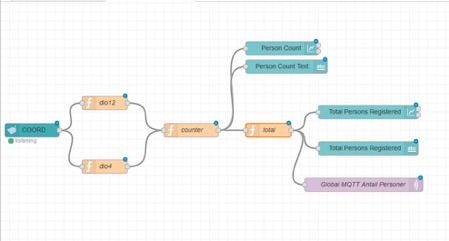
\includegraphics[width=0.8\textwidth]{personteller1}
  \caption{Node-RED flow brukt i Versjon 1 av personteller}
\end{figure}


COORD\cite{coord} modulen er en Node-RED XBee modul som lytter etter XBee meldinger i seriell porten på f.eks en Raspberry Pi, den sender så videre ut meldingen til de to funksjonene som ble laget for å filtrere ut hvilken PIR sensor som ble utløst først.

Kode dio12/4:
\begin{lstlisting}[caption=dio12/4 node funksjon]

var xBeeDIO12 = msg.payload;
//extracting the state of the DIO12 pin
var dio12In = xBeeDIO12.digitalSamples.DIO12;
 
//checking if the PIR sensor tripped, and assigning a timestamp to it
if(dio12In === 1){
	var dateDIO12 = new Date();
	global.set("DateDIO12", dateDIO12.getTime());
}
msg.payload = dio12In;
return msg;
\end{lstlisting}

Counter:

\begin{lstlisting}[caption=Counter node funksjon]

//Checking if the sensors have tripped
if(msg.payload === 1){
	msg.payload = "";
	var time4 = global.get("DateDIO4");
	var time12 = global.get("DateDIO12");
	//defining the differance between the trips
	var diff = time4-time12;
	//defining the num of people in the room
	var count = context.get('count')||0;
	var totCount = context.get('totCount')||0;
	
//checking if the trips happened within 3s of eachother, and in what direction
	if(diff > 0 && diff < 3000){
    	count += 1;
    	totCount += 1;
    	// store the value back
    	context.set('count',count);
    	context.set('totCount', totCount);
    	global.set('totalCount', totCount);
    	msg.payload = count;
	}else if(diff < 0 && diff >-4000){
    	if(count >= 1){
        	count -= 1;
        	context.set('count',count);
        	msg.payload = count;
    	}
    	
	return msg;
}
\end{lstlisting}

Denne løsningen viste seg å være den beste måten å løse person teller oppgaven når vi måtte ta personvernlov inn i betraktning. Hvordan kommunikasjonsteknologi labben brukes og limitasjonene med PIR sensorene viste seg å gjøre denne løsningen relativt ubrukelig. Ettersom labben normalt sett brukes av grupper mennesker så ville ikke denne telleren kunne telle nøyaktige mengder mennesker, men mer grupper mennesker som beveger seg gjennom døren i intervaller på 5 sekunder. Dette var grunnet at når en PIR sensor oppdaget bevegelse og gikk høyt, så ville det ta 5 sekunder uten bevegelse før den gikk lavt. 

Når denne løsningen ble lagt frem for veileder, og begrensningene med den så ble vi bedt om å finne en bedre løsning på dette. Etter å ha lagt frem at den eneste måten å løse denne problemstillingen var ved å bruke kamera, så ble vi fortalt at det måtte finnes en måte rundt personvernloven slik at et kamera kan brukes.

\newpage 
\section{Person Teller}
Etter å ha fått implementert flere sensorer som benyttet Zigbee nettverket til å sende data videre ut på Internett via MQTT megleren, ble det bestemt å lage en person teller inn til rommet. Det er et såpass mange med tilgang til dette aktuelle rommet at man ikke anser det som mulig å identifisere enkeltindivider, selv i samsvar med annen data som liste over personer med tilgang. En mener derfor at det ikke er nødvendig med de ekstra forholdsregler rundt personvernet som tidligere beskrevet.

\subsection{Personteller med PIR sensorer}
Når denne oppgaven ble utdelt så ble det kommunisert hvor viktig det var at det ble tatt høyde for personvernloven før noe ble satt opp i laboratoriet. Etter å ha utdypt oss i disse lovene så ble det klart at å bygge en person teller ved bruk av kamera kunne skape konflikter med personvernloven. Det ble da bestemt at person telleren skulle bygges ved bruk av xBee kort med PIR sensorer koblet til, og et koordinator xBee kort koblet til en Raspberry Pi.

Person telleren består av to xBee kort med hver sin PIR (Passive InfraRed-detektor) sensor i tillegg til en xBee koordinator koblet til Raspberry PI. Disse PIR sensorene er satt til å sende meldinger når de går høyt. Meldingene  sendes så videre til en koordinatoren og Raspberry Pi. Denne filtrerer ut overflødig informasjon, finner ut hvilken PIR sensor som gikk høyt, gir den en timestamp og sjekker deretter om den andre PIR sensoren har gått høyt og eventuelt gir timestamp dersom ja. Programmet vil da i praksis vite hvilken retning noen har beveget seg inn/ut av rommet, og kunne telle tilsvarende.

Årsaken til at det er brukt to xBee kort i stedet for ett med begge PIR sensorene tilkoblet er begrensninger på hastigheten xBee kortet klarer å prosessere og sende informasjonen. Ved 2 sensorer på samme xBee modul vil begge sensorene som regel oppdage bevegelse såpass raskt at xBee modulen melder begge høyt til Raspberry Pi som da vil sette lik timestamp. En mangler da informasjon på hvilke retning det dreier seg om.  

Det første problemet som viste seg var at vi ikke kunne koble 2 PIR sensorer til 1 XBee kort. Dette grunnet at når man har 2 PIR sensorer koblet til et XBee kort, så vil begge sensorene normalt sett oppdage bevegelse før XBee kortet kunne sende informasjonen videre. Noe som gjorde at å sette en timestamp på når de gikk høyt ikke ville gå, grunnet at etter meldingen fra XBee så gikk begge høyt samtidig. Dette problemet ble løst med å bruke 2 XBee kort, koblet med hver sin PIR sensor, og et koordinator XBee kort koblet til Raspberry Pi. 

\begin{figure}[!ht]
  \centering
      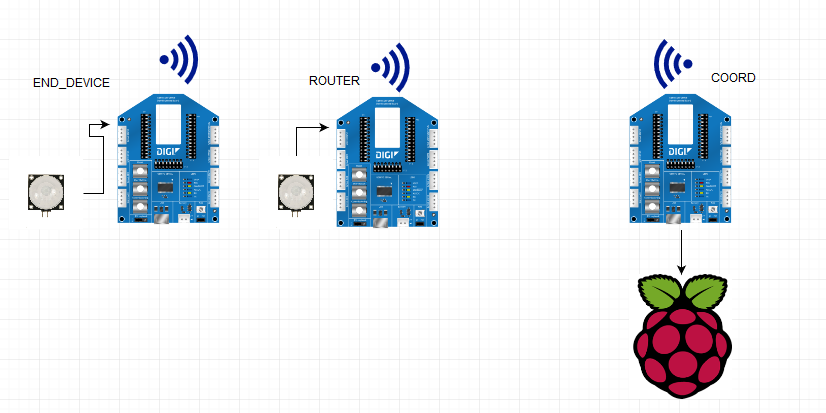
\includegraphics[width=0.7\textwidth]{PIRSetup}
  \caption{Illustrasjon av xBee Development Boards posisjonering}
\end{figure}

Her er Node-RED flowen som ble laget for denne oppgaven:
\\
\begin{figure}[!ht]
  \centering
      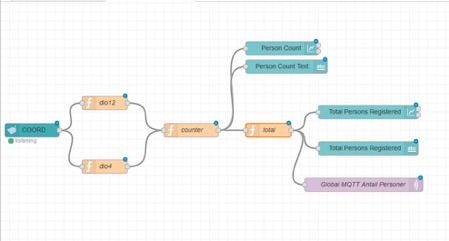
\includegraphics[width=0.7\textwidth]{personteller1}
  \caption{Node-RED flow for Versjon 1 av persontelleren}
\end{figure}

Koordinatoren, COORD modulen er en Node-RED XBee modul som lytter etter XBee meldinger i seriell porten på f.eks en Raspberry Pi, den sender så videre ut meldingen til de to funksjonene som ble laget for å filtrere ut hvilken PIR sensor som ble utløst først.

\begin{lstlisting}[caption=dio12/4 node funksjon]
var xBeeDIO12 = msg.payload;
//extracting the state of the DIO12 pin
var dio12In = xBeeDIO12.digitalSamples.DIO12;
 
//checking if the PIR sensor tripped, and assigning a timestamp to it
if(dio12In === 1){
	var dateDIO12 = new Date();
	global.set("DateDIO12", dateDIO12.getTime());
}
msg.payload = dio12In;
return msg;
\end{lstlisting}
I funksjonsnoden har det blir programmert inn logikk for telling av personer i JavaScript for å bestemme om en person går inn eller ut at rommet. Dette er gjort ved å hente inn data fra ZigBee netverket fra port DIO4 og DIO12 for så å tidsstemple når verdien blir innlest i millisekunder. Verdiene fra de forskjellige PIR sensorene blir her sammenlignet ved bruk av if-setninger for så å videresende det totale antallet til et Node-RED Dashboard og strømming via MQTT.
\begin{lstlisting}[caption=Counter node funksjon]
//Checking if the sensors have tripped
if(msg.payload === 1){
	msg.payload = "";
	var time4 = global.get("DateDIO4");
	var time12 = global.get("DateDIO12");
	//defining the differance between the trips
	var diff = time4-time12;
	//defining the num of people in the room
	var count = context.get('count')||0;
	var totCount = context.get('totCount')||0;
	
//checking if the trips happened within 3s of eachother, and in what direction
	if(diff > 0 && diff < 3000){
    	count += 1;
    	totCount += 1;
    	// store the value back
    	context.set('count',count);
    	context.set('totCount', totCount);
    	global.set('totalCount', totCount);
    	msg.payload = count;
	}else if(diff < 0 && diff >-4000){
    	if(count >= 1){
        	count -= 1;
        	context.set('count',count);
        	msg.payload = count;
    	}
    	
	return msg;
}
\end{lstlisting}

Denne løsningen viste seg å være den beste måten å løse person teller oppgaven når personvernlov ble tatt i betraktning. Hvordan kommunikasjonsteknologi laboratoriet brukes og begrensningene med PIR sensorene viste seg å gjøre denne løsningen relativt ubrukelig. Ettersom labben normalt sett brukes av grupper mennesker så ville ikke denne telleren kunne telle nøyaktige antall mennesker, men mer grupper som beveger seg inn og ut av rommet i intervaller på 5 sekunder. Grunnet at når en PIR sensor oppdager bevegelse og går høyt, så ville det ta ca. 5 sekunder uten bevegelse før den går lavt. 

Person telleren fungerer men med en begrensning på tidsintervallet mellom to registreringer. Denne begrensningen er på ca 5 sekunder og vil i praksis 

Når denne løsningen ble lagt frem for veileder, og begrensningene med den så ble vi bedt om å finne en bedre løsning på dette. Etter å ha lagt frem at den eneste måten å løse denne problemstillingen var ved å bruke kamera, så ble vi fortalt at det måtte finnes en måte rundt personvernloven slik at et kamera kan brukes.

\subsection{Personteller ved kamera og bildeanalyse}

Måten dette ble løst på var ved å ikke koble IP addresser opp imot bevegelse, og at all bildebehandling ville skje på et lukket nettverk, og ingen data utenom mengden mennesker i laboratoriet ville lagres. 

Vi fant ulike måter å løse denne oppgaven på ved bruk av kamera. Den første var Footfall https://github.com/WatershedArts/Footfall . Et program som registrerer bevegelse og lager ‘blobs’ med forskjellige ID-er for å kunne registrere inn- og utgang av f.eks en bygning. Denne løsningen brukte vi en del tid på, men fant etter en del feilsøking ut at dette programmet er laget for Debian Jessie, det gamle operativsystemet til Raspberry Pi som ble brukt før Debian Stretch ble sluppet 17 juni 2017. Om dette skal være en oppdatert IoT lab med den nyeste teknologien, så ble det besluttet at person telleren ikke kunne bruke Debian Jessie, og at det skulle søkes videre for å finne en løsning som støtter Debian Stretch.

Den neste programvaren som viste seg å støtte Debian Stretch, og kunne behandle live video og mønstergjenkjenning var OpenCV (Open Source Computer Vision). Som er et bibliotek av programmerings funksjoner hovedsaklig laget for å behandle real-time computer vision. Computer vision er i bunn og grunn et felt som undersøker hvordan man kan få en pc til å forstå bilde eller video. I perspektivet til ingeniører, så er formålet med computer vision det å automatisere det som det menneskelige visuelle systemet kan gjøre. 

Dette biblioteket av funksjoner kan behandle videofiler eller live-video og kunne følge bevegelse av objekter. Denne programvaren kan utnyttes av oss for å kunne loggføre aktiviteten inn og ut av kommunikasjonsteknologi laboratoriet. 

\subsubsection{Installasjon}
En veldig stor hindring med å implementere OpenCV var hvor vanskelig det var å installere på Raspberry Pi-en. Første gangen tok dette oss 3 dager med arbeid, og etter 3 dager med testing så krasjet Raspberry Pi-en og vi ble tvunget til å inngå 2 nye dager med installasjoner. OpenCV ble installert i en virtuell maskin i Raspberry Pi-en, dette grunnet at OpenCV har visse krav til programmer i bestemte versjoner. Mens et annet program på Raspberry Pi-en vil kanskje trenge en mer oppdatert versjon, denne konflikten løses med å laste ned de forskjellige versjonene på forskjellige virtuelle maskiner. 

Det neste problemet vi møtte på var at OpenCV ikke er designet for å ta input fra et Raspberry Pi Camera, et kamera spesielt designet for å være koblet til en Raspberry Pi. Dette ble løst med å importere en package som heter imutils, og kjøre følgende kode:
\begin{lstlisting}[language=Python, caption=OpenCV 1]

# konstrukter argument og parse argument
ap = argparse.ArgumentParser()
ap.add_argument("-p", "--picamera", type=int, default=-1,
    help="whether or not the Raspberry Pi camera should be used")
args = vars(ap.parse_args())
 
# Start video stream og la kamerasensor varme opp
vs = VideoStream(usePiCamera=args["picamera"] > 0).start()
time.sleep(2.0)
\end{lstlisting}

Når input fra kameraet kunne behandles, måtte programmet kunne skille mellom hva som var bakgrunn, og hva som var bevegende objekter over bildet. Dette kan OpenCV gjøre ved å kalle en funksjon som kalles “background subtracting”. En funksjon som tar inn hele bildet, gjenkjenner hva som aldri er i bevegelse, og definerer det som bakgrunn.

\begin{lstlisting}[language=Python, caption=OpenCV 2]

fgbg = cv2.createBackgroundSubtractorMOG2(detectShadows = True)

fgmask = fgbg.apply(frame)
\end{lstlisting}


Deretter oppstår problemet hvor skygger som beveger seg over bildet vil også bli registrert som bevegende objekter. Noe som kan gjøres i OpenCV er det at man kan utnytte to funksjoner som heter dilate og erode\cite{opencvdos}, til å kunne filtrere ut skygger som beveger seg sammen med menneskene. 
\begin{figure}[!ht]
  \centering
      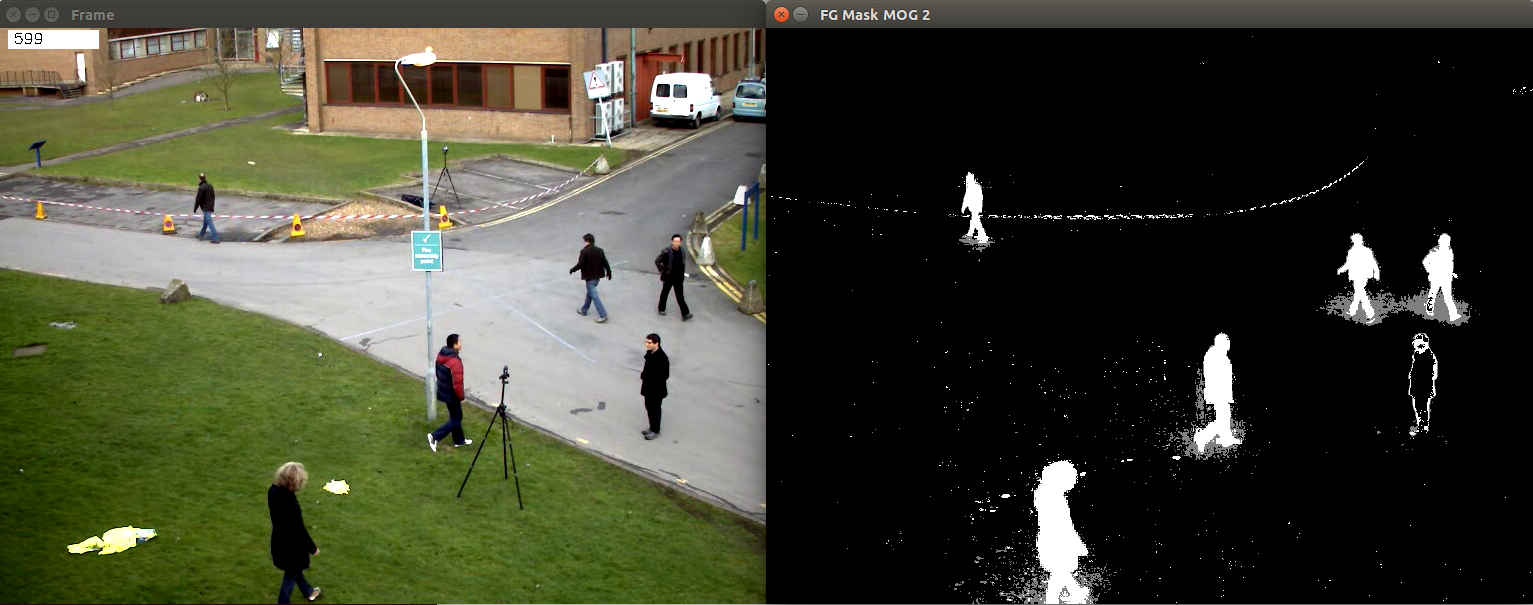
\includegraphics[width=0.7\textwidth]{opencvBackgroundSubtraction}
  \caption{OpenCV analyse eksempel}
\end{figure}
Om dette ikke ble gjort så kunne bevegelsen av skyggen foran/bak menneske registrere som et eget menneske og telle dobbelt, eller forvirre sensoren om hva den skal definere som menneske eller ikke. Dette gjøres:

\begin{lstlisting}[language=Python, caption=OpenCV 3]
# Lage bakgrunn som kan trekkes fra video stream
kernelOp = np.ones((3,3),np.uint8)
kernelCl = np.ones((11,11),np.uint8)
#Erode -> Dilate
mask = cv2.morphologyEx(imBin, cv2.MORPH_OPEN, kernelOp)
mask2 = cv2.morphologyEx(imBin2, cv2.MORPH_OPEN, kernelOp)
#Dilate -> Erode
mask =  cv2.morphologyEx(mask , cv2.MORPH_CLOSE, kernelCl)
mask2 =  cv2.morphologyEx(mask2 , cv2.MORPH_CLOSE, kernelCl)
\end{lstlisting}

Når kameraet har filtrert ut så mye skygger som mulig, så kan programmet kunne tegne en grense rundt det som beveger seg.

\begin{lstlisting}[language=Python, caption=OpenCV 4]
_, contours0, hierarchy = cv2.findContours(mask,cv2.RETR_EXTERNAL,cv2.CHAIN_APPROX_NONE)
for cnt in contours0:
   	 cv2.drawContours(frame, cnt, -1, (0,255,0), 3, 8)
\end{lstlisting}

\begin{figure}[!ht]
  \centering
      
\includegraphics[width=0.7\textwidth]{dilationErosion}
  \caption{Forbedring av bevegelseslesning OpenCV eksempel}
\end{figure}

Deretter må arealet av det bevegende objektet regnes ut, for å sjekke om det er stort nok til å defineres som et menneske:
\begin{lstlisting}[language=Python, caption=OpenCV 5]

	area = cv2.contourArea(cnt)
    	if area > areaTH:
   		 ##################
   		 #   TRACKING	#
   		 ##################
   		 M = cv2.moments(cnt)
   		 cx = int(M['m10']/M['m00'])
   		 cy = int(M['m01']/M['m00'])
   		 x,y,w,h = cv2.boundingRect(cnt)
\end{lstlisting}

Her tegnes det et rektangel rundt objektet som skal defineres som en person, og det begynner å bli fulgt. Deretter må programmet kunne telle, her sjekker det om objektet er innenfor de linjene som defineres som line\textunderscore down og line\textunderscore up. 

\begin{figure}[!ht]
  \centering
      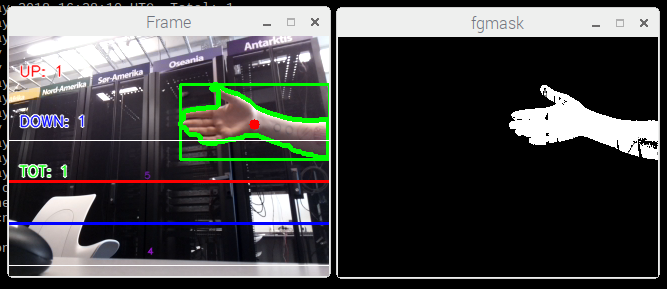
\includegraphics[width=0.7\textwidth]{fgmask2}
  \caption{Eksempel på linjer som reggistrerer personer inn og ut}
\end{figure}

To linjer som brukes til å regne ut hvilken retning objektet beveger seg i. Når det vet hvilken retning det beveger seg i så itereres cnt\textunderscore up eller cnt\textunderscore down og total. 
\begin{lstlisting}[language=Python, caption=OpenCV 6]

if cy in range(up_limit, down_limit):
	for i in persons:
		if abs(cx-i.getX()) <= w and abs(cy-i.getY()) <= h:
			new = False
			i.updateCoords(cx,cy)
			if i.going_UP(line_down,line_up) == True:
				cnt_up += 1
				total += 1
				print("Person:",i.getId(),'Gikk inn ',time.strftime("%c"),' Total:', str(total))
			elif i.going_DOWN(line_down,line_up) == True:
				cnt_down += 1
		if total >=1:
			total -= 1
		else:
			total = 0
			print("Person:",i.getId(),'Gikk ut ',time.strftime("%c"),' Total:', str(total))	
\end{lstlisting}

Når et objekt har blitt talt, eller det beveger seg av skjermen, så må personen slettes, og fjernes fra persons matrisen:
\begin{lstlisting}[language=Python, caption=OpenCV 6]

if i.getState() == '1':
   	if i.getDir() == 'down' and i.getY() > down_limit:
   		 i.setDone()
   	 elif i.getDir() == 'up' and i.getY < up_limit:
   		 i.setDone()
if i.timedOut():
   	 index = persons.index(i)
   	 persons.pop(index)
   	 del i
\end{lstlisting}

\subsubsection{Sending av data til Internett og Node-RED Dashboard}
Etter implementering av logikken, oppkobling av utstyr og enkel avlusning er det neste steget å gjøre persontelleren en del av IoT laboratoriet. Dette har blitt gjort ved å sende data gjennom MQTT protokollen til  Raspberry Pi gatewayen allerede oppkoblet på laboratoriet. Videre blr data sendt til et Node-RED Dashboard sammen med resten av miljøovervåkningen for laboratoriet. Data grafes og skrives ut som en ren tekst verdi.  Som nevnt tidligere i rapporten har vi bruk Paho MQTT og Mosquitto for sending av MQTT gjennom Python. 

\begin{lstlisting}[language=Python, caption=Paho MQTT tilkobling av klient]

client = mqtt.Client("python_pub")
client.username_pw_set(username="pi", password="raspberry")
client.connect("192.168.1.38", 1883) 
client.loop_start()
\end{lstlisting}

Data som sendes til RPi IoT Gatewayen er data fra en total variabel lenger inn i Python programmet. Ved å plassere oppdateringen i While løkka som oppdateres for hver lesning vil antall personer i bli raskere oppdatert. Det vil ikke by på problemer med strømmforbruk da hele opsettet har strømmforsyning fra stikkontakt ikke baterier.
\begin{lstlisting}[language=Python, caption=Publisering av antall personer til IoT Gateway via Paho MQTT i Python]
client.publish("personteller/antall",str(total))
\end{lstlisting}

\subsubsection{Begrensninger}

Den største begrensningen vi møtte på ved implementasjonen av denne person telleren var at all den beste testingen kunne kun skje på et sted hvor Raspberry Pi-en kunne være koblet til en skjerm. Grunnet at denne linjen \textbf{cv2.imshow("Frame", frame)}. Som får en ramme til å dukke opp som viser hva som defineres som mennesker, og kan vise hvor problemer skjer, kan ikke åpnes via SSH. Dette har ført til venskeligheter med avlusing og forbedring av kode.

\subsubsection{Diskusjon rundt bruk av kamera}
Ved å bruke et kamera som filmer bevegelser og et program som bearbeider video, vil det være mulig å identifisere enkeltindivider. Under eksperimentering med flytting av kamera på laboratoriet kom det fram at identifisering av personer er uunngåelig. Dette medfører da også spørsmål rundt personvern. 

Raspberry Pi som tar seg av bildeprosessering er plassert rett ved kamera over døren. Bildet fra kamera sendes derfor ikke over nettverket men behandles lokalt. Det eneste som sendes fra Raspberry Pi er altså telle verdien. Bildene blir ikke lagret men er direkte behandlet. Det er heller ikke mulig å logge seg inn på Raspberry Pi annet enn lokalt. Dette er på grunn av at cv2.imshow("Frame", frame) ikke kan åpnes via SSH. Av disse årsaker mener en direkte behandlede bilder er godt nok beskyttet. 

\subsubsection{Forbedringer fra Versjon 1}
Denne løsningen bedre enn den første versjonen med PIR sensorer men har fremdeles noen begrensninger. Er det en gruppe med personer som er veldig nære hverandre så vil det registreres som en person inn/ut av laboratoriet. Kommer personen i stor fart så vil ikke Raspberry Pi-en kunne registrere, tegne en grense og telle den personen tidsnok. I vanlig tempo er ikke dette noe problem. 






%----------------------------------------------------------------------------------------
%   DISKUSJON SEKSJON
%----------------------------------------------------------------------------------------

\newpage
\section{Diskusjon}

\subsection{Utvidelse av Lab}

Det er flere muligheter for å oppgradere denne IoT labben, og i denne oppgaven har vi hatt fokus på at dette skal gå så knirkefritt som mulig. I denne delen av rapporten skal vi se på de forskjellige oppgraderingsmulighetene vi ser på som aktuelle, og hvorfor. Vi har valgt å begrense denne delen til å kun omhandle videre bygging på den allerede klargjorte infrastrukturen på nettverks labben. Med andre ord utelater vi muligheten for  implementere flere av protokollene som blir brukt innenfor IoT feltet. Dette er fordi denne delen av rapporten da hadde blitt for lang, og det ville gått forbi oppgaven vi har fått definert. 

\subsubsection{Flere Raspberry Pi enheter og innkjøp av Sense Hat}

Den oppgraderingen av IoT labben som vi mener er den mest aktuelle er enkelt og greit å kjøpe inn flere Raspberry Pi med sensor tilkoblingen Sense Hat som også er levert av Raspberry Pi. Grunnen til dette er at det er en veldig effektiv måte å illustrere grunnprinsippene i IoT, det krever lite forkunnskap både innenfor programmering og sensorteknikk samt at det er en løsning som kan vekke kreativitet og læringsglede hos studentene.

En Raspberry Pi bruker i første omgang WiFi for sending av data ut, men kan også brukes til å kommunisere med Bluetooth enheter. Dette gjør den fleksibel og aktuell, da WiFi er en av de mest brukte standardene innen IoT. Dersom man kobler på en Sense Hat vil det være en effektiv måte å illustrere hvordan sensor data hentes inn, bearbeides, går gjennom nettverket og ut på internett. Dette er noe vi mener kan hjelpe studenter å forstå hvordan flere av fagene i data studiet henger sammen, og gjør programmering, databaser, nettverk og sensor data til noe litt mindre abstrakt.

Grunnen til at det vil kreve lite forkunnskap er at produktet Sense Hat er utviklet av Raspberry Pi for læring. Det vil si at det allerede er laget fler Python biblioteker som lett kan installeres og tas i bruk. Dette minimerer mengden programmering en student  må kunne før oppgaven starter. Det er også lett å koble til Sense Haten, man setter den enkelt på GPIO pinnene på Raspberry Pi. Det er ikke behov for å koble inn motstand eller strøm de den er spesiallaget for Raspberry Pi. Dette fjerner da behovet for forkunnskaper innenfor sensorteknikk. 

I tillegg til å være lett å bruke har en Sense Hat flere nyttige egenskaper, den måler temperatur, luftfuktighet, barometrisk trykk, har akselerometer, gyroskop og en 8x8 RGB LED matrise. Alle disse sensorene kan lett tas i bruk gjennom Raspberry Pis Python bibliotek. Dette vil gi stor frihet i konstruering av oppgaver, og dette også data som vil kunne brukes i fag som for eksempel Websearch og Datamining. Med andre ord vil en Sense Hat by på fleksibilitet i vanskelighetsgrad og omfang av oppgaver. Noe som gjør at den kan brukes av både nye studenter og studenter som allerede er godt kjent med nettverk og programmering. Om universitetet ønsker vil det også kunne brukes som en del av en IoT lekeplass der studenter kan eksperimentere med teknologien og lære på egenhånd. 


\subsubsection{Flere xBee Development Boards og flere xBee antenner}
Dersom UiS sin IoT lab skal utvides videre kan det være aktuelt å legge et større fokus på ZigBee protokollen. En god måte å gjøre dette på vil være å kjøpe inn flere xBee Development Kits levert av Digi og flere xBee antenner. Dette er den enkleste måten å utvide mulighetene for testing av allt ZigBee har å tilby. Dersom universitetet hadde hatt flere slike pakker ville vi unne utforsket for eksempel ZigBee sine mesh nettverk muligheter dypere. En annen mulighet ville ha vært å koblet til flere forskjellige sensorer til xBee modulene og antennen, for så å plassere dem over universitetet for å lage et større mesh nettverk som henter inn flere typer data. Dette vil gi muligheten til å hente ut data om hvor mange som befinner seg i hvilke deler av universitetet basert på for eksempel luftkvalitet og bevegelse. Noe som vil kunne brukes som en del av pensum i fag som er relatert til data mining og big data. Ved innkjøp av enkle antenner og utvikler kort, vil også en student for eksempel kunne slå på kaffetrakteren inne på et annet rom ved å åpne tilgang til strøm. Alle disse bruksområdene og mange flere vil man kunne utforske ved å kjøpe inn flere antenner og utvikler kort. Det vil så klart ikke være nødvendig å holde seg til Digi sine pakker, det vil også være mulig å bruke den noe mer fleksible Arduino Uno til samme formål. Det vil da også føre til mer sensor teknikk og programmering i språk som ikke er obligatoriske ved UiS. 

Pakkene med utvikler kort gjør det mulig å tilkoble sensorer til antennen på en enkel måte som fjerner krav om forkunnskap rundt sensorteknikk. 


\subsubsection{Microsoft Azure IoT Hub}
Neste steg i bygging og forbedring av IoT labben vil det være aktuellt å implemementere Microsoft Azure sin IoT Hub. Dette vil gi mulighet for utforskning av dypere analyse av data og for testing av sky tjenester. Bruk av for eksempel Microsoft Azure sin MQTT Cloud Server vil kunne muliggjøre for eksempel fjernstyring av utstyr på labben på en relativt trygg måte. Ved bruk av denne skytjenesten vil man også kunne skru av og på xBee moduler, disse kan bli brukt til å styre allt fra kaffetraktere til lys. Det er også et argument for at Azure sin struktur vil gi studentene en mer strømmlinjeformet læringsprosess, selv om fokuset vil bli mindre akademisk. Med mindre akademisk, menes et svakere fokus på tekniske detaljer som for eksempel tildeling av IP-adresser, bruk av terminaler for konfigurering og programmering. 

Dersom man ser bort fra noen av ulempene med Microsoft Azure, er det et bra verktøy for behandling av data fra IoT labben vår. Azure kan også være med på å skape interesse for IoT, da man lett kan sette opp sitt eget miljø. Et eget miljø kan ha data fra temperatursensorer hjemme, der man får for eksempel SMS dersom temperaturen i stua stiger over en gitt temperatur, eller et overvåkningskamera avgarasjen som tar bilder om det registrer bevegelse. 

\subsection{Utfordringer med MQTT}
Ved implementasjon av MQTT protokollen kommer noen utfordringer, spesielt med hensyn til sikkerhet og til bruk på en lukket Lab. Det er viktig å være klar over utfordringene som kan komme ved bruk av protokollen, og potensielle løsninger. 

\subsubsection{Sikkerhets utfordringer med MQTT}
Måde den TCP baserte MQTT protokollen og den UDP basert MQTT-SN protokollen har noen utfordringer når det kommer til sikkerhet, flere av disse har oppstått da protokollen originalt er bygd for implementasjon på backend. Sikkerhets utfordringene oppstår ofte på grunn av selve bruksområdet, som er IoT, hvor kravet til lavt strømforbruk, liten bruk av båndbredde og samtidig rask sending av data er viktig. Det vil være mulig å konfigurere SSL/TSL sertifikater for sending over protokollene, men dette blir ofte ikke gjort av disse grunnene. I tillegg er SSL/TSL sårbart for angrep fra BEAST, CRIME, RC4, Heartbleed og lignende. IoT enheter er ofte mange og relativt like enheter, dette skaper også problemer med lagring og styring dersom det for hver sending kreves SSL/TSL sertifikater.

Det finnes foreløpig ikke noen løsning på dette, og behovet for en robust og skalerbar mekanisme for sikring av nettverk som krever lite strøm og databruk er voksende. Som en potensiell løsning har det blitt designet utkast til oppgradering av SMQTT, en sikrere versjon av MQTT. Dette har ikke blitt implementert i praksis enda, men kan være en løsning på noen av sikkerhetshullene protokollene har. Andre protokoller som CoAP har samme sikkerhetsproblemer som MQTT, problemene oppstår fordi IoT nettverk har spesielle krav.

\subsubsection{Sending til Internett}
MQTT protokollen har problemer med sending til Internett dersom man ikke ønske å åpne brannmuren på nettverket og åpne for port forwarding eller ta i bruk en skytjeneste som Microsoft Azure. Det er ikke mulig å sende MQTT data fra en Raspberry pi som fungerer som megleren på IoT labben uten port forwarding da den ikke har en offentlig tilgjengelig IP-adresse. Her åpner det et sikkerhetshull om man åpner portene på Unix nettet for å muliggjøre dette. Som en funksjon av dette vil ikke labben kunne brukes til akkurat dette formålet. Det vil være mulig å sende MQTT data ved bruk av en skytjeneste om personer som bruker labben har konfigurert dette selv, dette er den eneste muligheten for sending av MQTT data til Internett.


\subsection{Navnestandarder}
Med hensyn til brukervennlighet har vi valgt å implementere en navnestandard som samsvarer med den som allerede er på lab. Det er viktig å ha en lett forståelig navnestandard, sånn at studenter lett vil kunne forstå hvilke nettverk som tilhører IoT labben, og hvilke som er tilgjengelige for alle. Vi har derfor valgt å kalle WiFi nettverket Komtek\textunderscore IoT\textunderscore A for enkelthets skyld. Routere vil bli kallt komtekiotrouter, og switcher komtekiotswitch. Det er ikke mulig å sette en navnestandard på ZigBee nettverket, dette er fordi nettverket defineres med tall.
\newpage
\subsection{Organisering av arbeid}
\subsubsection{Gantt-diagram og Timelister}
Som et viktig verktøy for å holde kontroll på fremmgangen av prosjektet, og når forskjellige stadier av oppgaven skal være ferdig har vi tatt i bruk Gantt-diagrammer. Vi har startet bruken av disse allerede fra første uke, og funnet dette til å være en effektiv måte å holde flyt i arbeidet. Grunnen til dette er at man enkelt kan se ut fra diagrammet når en del av prosjektet må være ferdig for at en annen skal kunne startes. Denne måten å organisere arbeid paret med test drevet utvikling har vært med på å skape god fremmgang. Gantt-diagrammet har blitt oppdatert ukentlig, da noen deler av oppgaven har tatt kortere tid en forventet og andre lenger. 

\begin{figure}
  \centering
      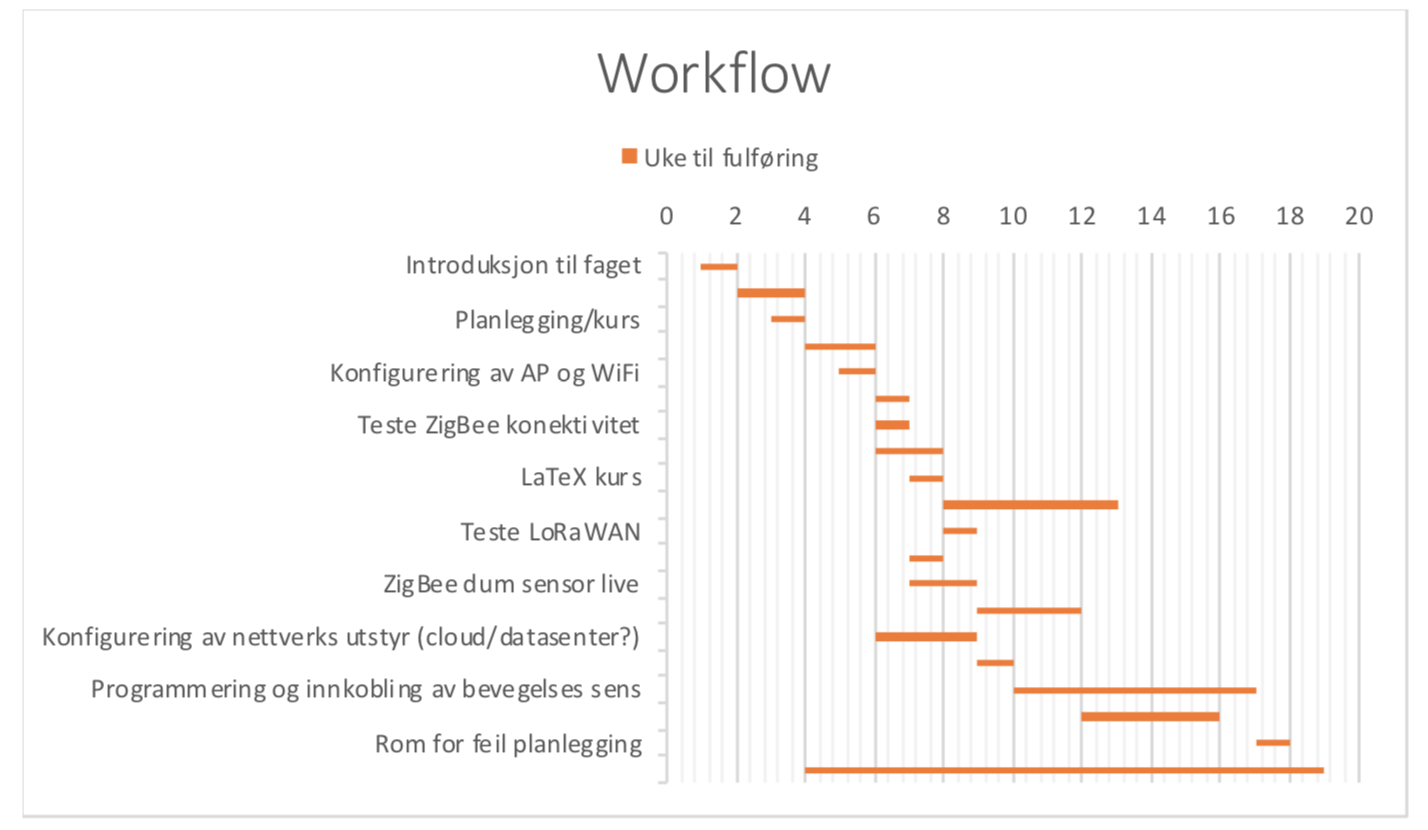
\includegraphics[width=0.9\textwidth]{gantt}
  \caption{Her ser vi et eksempel på Gantt-diagrammet vårt. Det er inndelt i uker, og har oppgaver som skal fulføres innen den gitte uken.}
\end{figure}

Som et supplement til Gantt-diagrammet har vi valgt å føre timer for å forsikre oss om at vi legger in et minimum av 35 timer hver uke. Dette har også vært et nyttig verktøy for å holde system i oppgaven under veis. Vi har valgt å knytte arbeidsoppgaver til timene, og å skrive korte notater fra dagen etter hver dag. Dette har vært for å enklere kunne oppdatere Gantt-diagrammet og for enklere rapportskriving. 

\subsubsection{Scrum, Kanban og testdrevet utvikling}
Scrum og Kanban er måter å organisere prosjekter der det er viktig å holde en jevn flyt gjennom hele prosjektet. Både Scrum og Kanban er smidige prosesser som ofte blir satt opp mot hverandre, men vi har valgt å kombinere begge under organisering av arbeidet\cite{scrumandkanban}. Som et bakteppe for Scrum og Kanban har vi benyttet oss av testdrevet utvikling. Testdrevet utvikling er å løse det letteste senarioet for en problemstilling som overhode mulig, for så å jobbe seg gjennom vanskeligere scenarioer før man tilslutt har et ferdig produkt. Dette er for å minimere dødtid, og for å lettere finne ut om en måte å løse et problem ikke virker så fort som mulig. Denne måten å strukturere arbeidsprosessen har vist seg relativt effektiv.

\begin{figure}
  \centering
      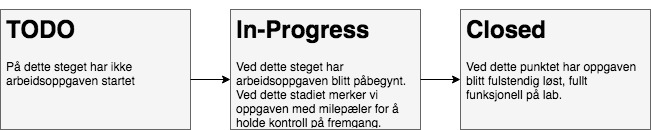
\includegraphics[width=0.9\textwidth]{ScrumKanban}
  \caption{En arbeisoppgave går gjennom tre stadier, TODO, In-Progress og Closed, alle dokumenteres på GitHub}
\end{figure}

\subsubsection{GitHub, Google Drive og Cisco Spark}
GitHub, Google Drive og Cisco Spark har alle vært viktige komponenter i strukturering av arbeid og for reserve kopier av filer. Cisco Spark er et verktøy utviklet av Cisco for deling av filer, organisering av arbeid og chatting. Her kan man lage områder til for eksempel et front-end team og et til backend team. Dette ble brukt for oppdatering av veiledere på fremdrift sammen med møter.

Google Drive er en skybasert tjeneste for lagring og deling av filer. Det benytter seg av Googles eget rammeverk og egne programmer for laging av presentasjoner, tekstdokumenter og så videre. Ved å bruke Google Drive, for så å lagre kopier lokalt på maskinen beskytter man data om en av maskinene skulle havarere.

GitHub og Git er versjonskontrollsystem som ofte blir for organisering og kontrollering av fil versjoner. GitHub kan også brukes som en wiki for informasjon og strukturering av arbeid ved bruk av GitHub Issues. Under organisering av oppgave har alle funksjonene nevnt her blitt tatt i bruk. GitHub Issues har vist seg å fungere veldig bra i organisering sammen med Scrum og Kanban.

\begin{figure}
  \centering
      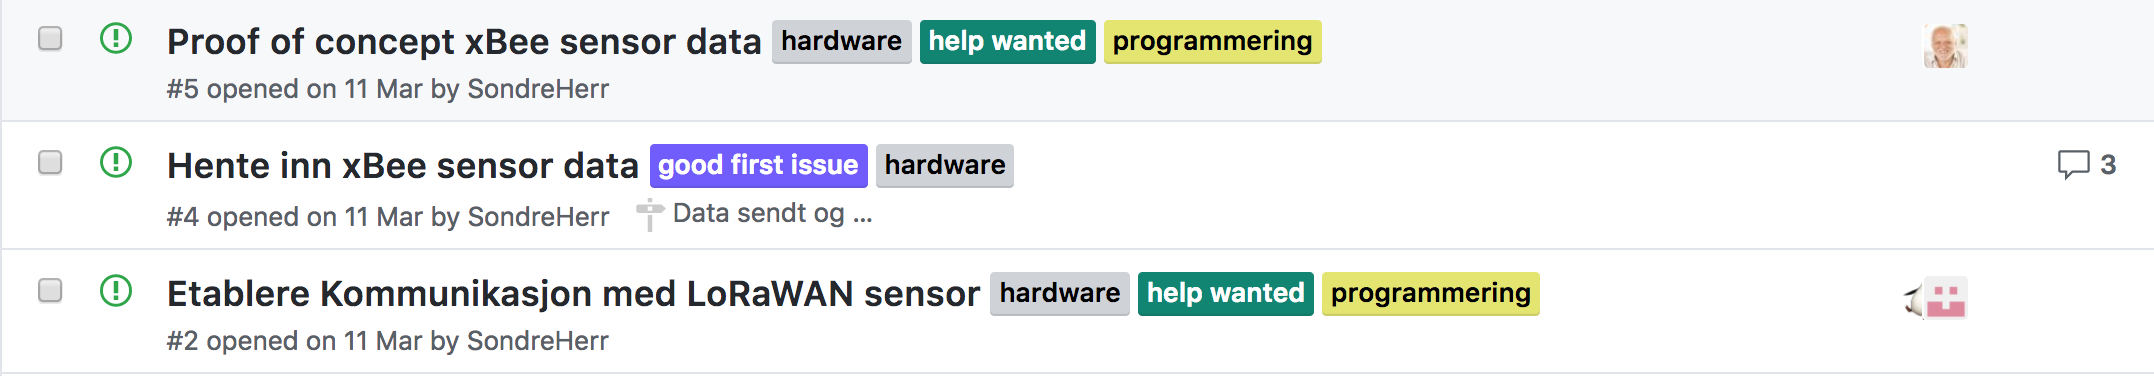
\includegraphics[width=0.9\textwidth]{GitHubIssues}
  \caption{Eksempel på bruk av GitHub Issues}
\end{figure}

\subsection{Sammendrag}
Som IoT labben står, vil det være mulighet for videre utvidelse og implementering av flere teknologier. Her er det mulig å lage andre IoT baserte Bachelor, Master og PhD prosjekter på lik linje som det er mulig for studenter å teste egne ideer. Det vil videre for eksempel være morsomt å lage en IoT applikasjon for samling av all data fra forskjellig protokoller, og nærmere analysere for eksempel forholdet mellom antall personer i rommet og luftkvalitet. Eller SMS basert varsling for når det er få mennesker i laben under øvingstimer i Kommunikasjonsteknologi. 


\newpage
\begin{appendices}
\appendix
\section{\\Hvordan nå RPi via SSH}
Finn ip adressen til Raspberry Pi-en:
Dette kan gjøres ved kommandoen hostname -I, da vil man få opp ip adresse og MAC adresse på enheten.
\\
Åpne Putty og velg ssh, port 22.
Forsikre deg om at du er på samme wifi nettverk som RPi.
Default brukernavn på en RPi er pi, passord er satt til raspberry
\\
Dersom du har en Mac, kjør denne kommandoen fra Terminal:
ssh 192.168.1.12 -p 22 -l pi
\\
Denne kommandoen er på formatet:
ssh \textbf{ip adresse} -p \textbf{portnummer} -l \textbf{brukernavn}

\begin{table}[!ht]
	\centering
	\caption{Relevante parametere for SSH sesjon med RPi}
	\begin{tabular}{|l|l|}
		\hline
		\textbf{Brukernavn} &  pi\\ \hline
		\textbf{Passord} & raspberry \\ \hline
		\textbf{SSH port} &  22\\ \hline
		\textbf{IP-adresse} &  192.168.1.x\\ \hline
	\end{tabular}
\end{table}

\newpage 
\section{\\Hvordan sende SenseHat fra Raspberry Pi til Internett}
I denne oppgaven skal vi hente ut data fra sensorer, bearbeide data og sende det ut på Internett for så å bearbeide data. Vi skal ta i bruk en Raspberry Pi Sense Hat som sensor, men prinsippet her er det samme som for alle andre sensorer. I denne oppgaven vil dere bli bedre kjent med kommandolinjen, python programmering og henting av sensordata.
\\

\textbf{Oppgaven krever:}
\begin{itemize}
	\item Raspberry Pi
	\item Sense Hat
	\item Internett tilgang
	\item Python programmering
\end{itemize}


\begin{figure}[!ht]
  \centering
      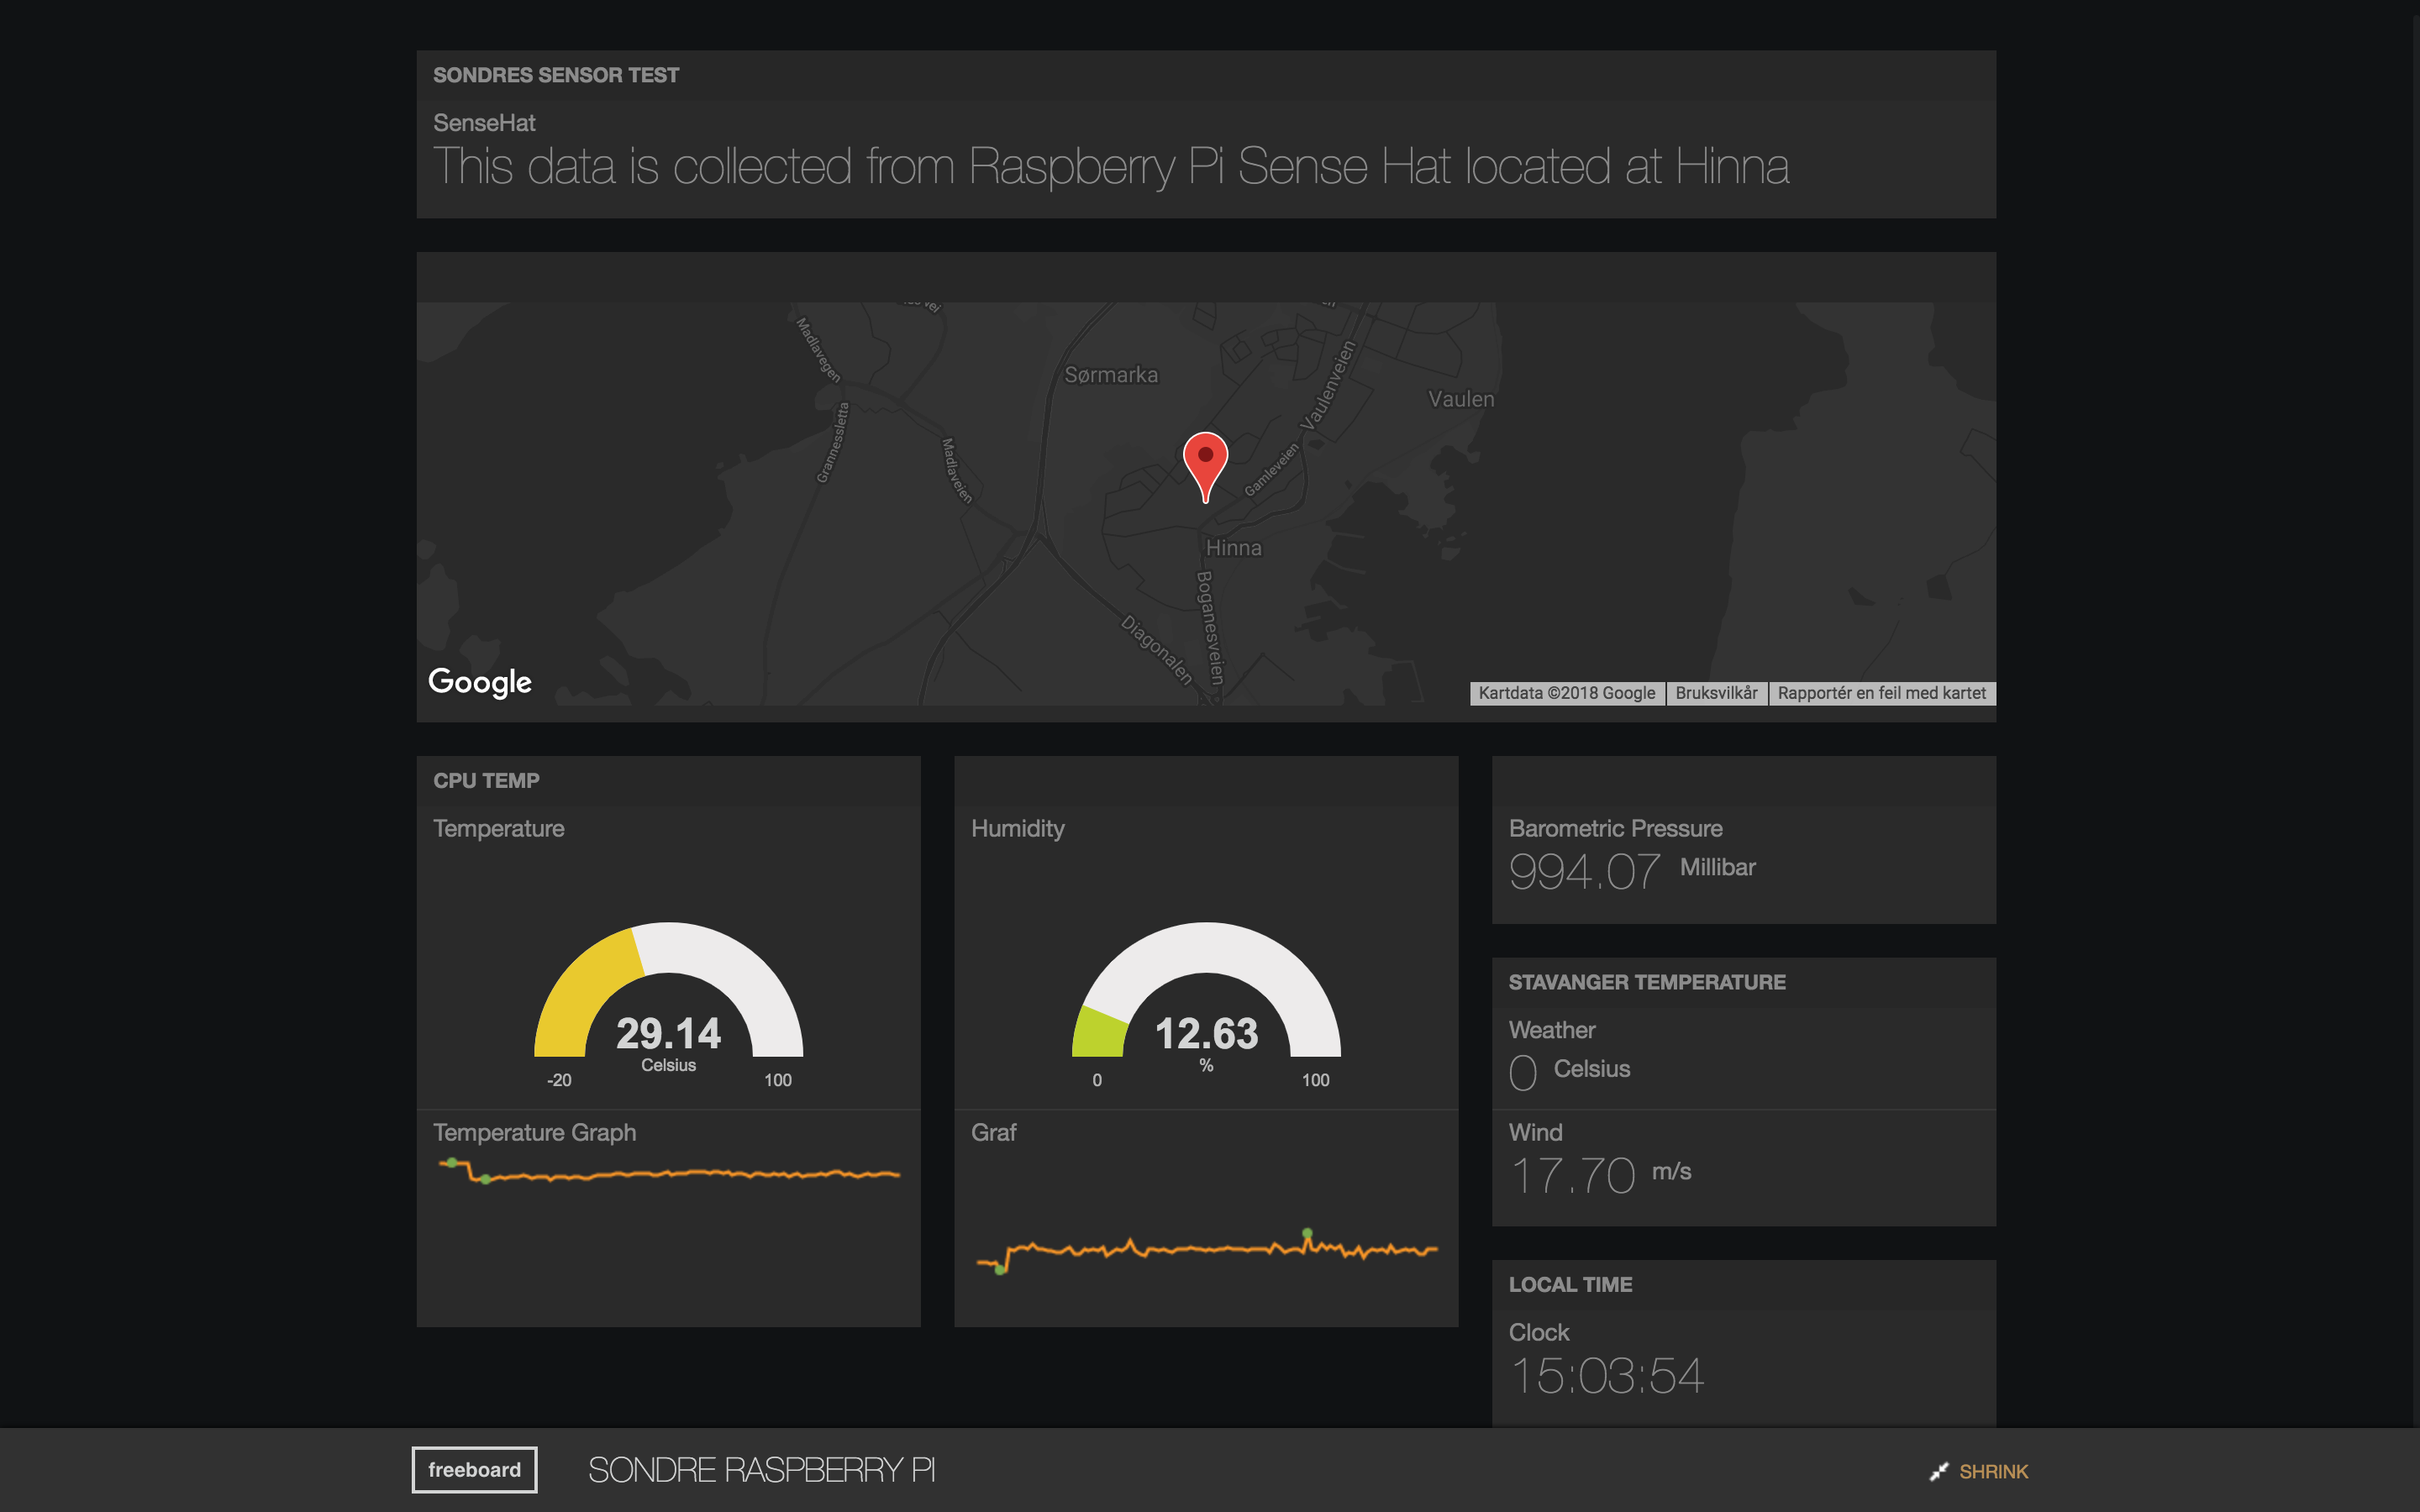
\includegraphics[width=0.9\textwidth]{appendixb}
  \caption{Appendix B Freeboard}
\end{figure}


\subsection{Steg 1}
I dette steget skal vi oppdatere Raspberry Pi og opprette en mappe og ei fil fra kommandovinduet/terminalen.
Koble opp Raspberry Pi til skjerm, mus og tastatur, og koble til Internett.
\\
Åpne terminalen og sørg for at enheten er oppdatert med kommandoene:
\begin{itemize}
	\item sudo apt-get update
	\item sudo apt-get upgrade
\end{itemize}


Skriv inn følgende kommandoer for å opprette ei mappe og fil
cd Documents/ denne kommandoen navigerer deg til Documents mappen
mkdir tempData denne kommandoen oppretter en mappe kalt senseHatData
sudo nano senseHatData.py denne kommandoen lager ei Python fil og åpner den i tekst verktøyet nano
Du er nå inne i filen senseHatData.py og er klar til å starte programmeringen
\\
Noen grunnleggende kommandoer i nano editoren og kommandolinjen:
\begin{itemize}
	\item ctrl + o lagrer fila
	\item ctrl + x avslutter
	\item ctrl + w søker
	\item ctrl + c avslutter et kjørende program
\end{itemize}

\subsection{Steg 2}

I dette steget skal vi skrive et kort Python program for innhenting og sending av data. I den vedlagte koden vil dere se en del print setninger, formålet med disse er å lettere kunne debugge koden og feilsøke om noe går galt.
NB: Python krever rett indentation for å kjøre riktig.

Start med å importere relevante biblioteker:
\begin{lstlisting}[language=Python, caption=ApendiX B del 1]
from sense_hat import SenseHat
import requests
import time
	\end{lstlisting}

Lagre så Sense Hat objektet i en variabel
sense = SenseHat()
Nå skal vi definere en funksjon som henter inn data fra sensorene på Sense Hat, avrunder tallene og konverterer tallene til strenger(String)
\begin{lstlisting}[language=Python, caption=ApendiX B del 2]
def readings():
temp = sense.get_temperature()
temp = round(temp, 2)
temp_str = str(temp)
print("Temperature in C: ", temp)

	humidity = sense.get_humidity()
	humidity = round(humidity, 2)
	humidity_str = str(humidity)
	print("Humidity: " , humidity)
	
	pressure = sense.get_pressure()
	pressure = round(pressure, 2)
	pressure_str = str(pressure)
	print("Pressure: ", pressure)
	print("Str: ", pressure_str)
	\end{lstlisting}

Til slutt i funksjonen trenger vi å skrive data til en url for å sende ut til internett. For så å poste data, ved bruk av python biblioteket requests og post(). Det er viktig at denne delen kommer nederst da man ikke kan skrive ut en variabel som ikke oprettet.

\begin{lstlisting}[language=Python, caption=ApendiX B del 3]

url = "https://dweet.io/dweet/for/dinIdentifikator?" + "Temperatur=" + temp_str + "&Humidity=" + humidity_str + "&Pressure=" + pressure_str
r = requests.post(url)
\end{lstlisting}


Erstatt dinIdentifikator i url variabelen til hva som helst. Dette vil være identifikatoren til din stream hos dweet. Du er nå ferdig med funksjonen for innhenting av data. 
Det gjenstår nå å kjøre funksjonen vi nettopp har lagd sånn at vi henter inn sensor data med rimelige mellomrom. Vi gjør dette ved å bruke en while loop og hente data hvert 10 sekund.

\begin{lstlisting}[language=Python, caption=ApendiX B del 4]
while True:
	readings()
	time.sleep(10)
	print("Readings recorded")
\end{lstlisting}
Programmet lagres med \textbf{ctrl + o}, og man avslutter nano ved \textbf{ctrl + x}
Programmet kan kjøres med kommandoen: \textbf{sudo python senseHatData.py}

Dersom alt gikk som det skulle kan du se om data ble publisert her: http://dweet.io/follow/dinIdentifikator

\subsection{Steg 3}

I dette steget skal vi ta i bruk freeboard.io, som er en sammarbeidspartener med dweet.io lagd for iot utviklere sitt grensesnitt til å sette opp et dashboard.

Opprett en bruker her: https://freeboard.io/signup

Når du har gjort dette vil du kunne lage et eget dashboard. Velg et passende navn og trykk \textbf{Create New}.

\subsection{Steg 4}

I dette steget skal vi lage et dashboard som fremstiller data.

Du er nå inne på ditt nye dashboard. Velg så Add  Data Source  Dweet. Dette vil muligjgjøre henting av data fra dweet.io siden vi har sendt data til tidligere. 

\begin{lstlisting}[language=Python, caption=Hvordan sende temperaturdata fra Raspberry Pi til Internett Fasit Kode]
from sense_hat import SenseHat
import requests
import time


sense = SenseHat()

def readings():
	temp = sense.get_temperature()
	temp = round(temp, 2)
	temp_str = str(temp)
	print("Temperature in C: ", temp)

	humidity = sense.get_humidity()
	humidity = round(humidity, 2)
	humidity_str = str(humidity)
	print("Humidity: " , humidity)

	pressure = sense.get_pressure()
	pressure = round(pressure, 2)
	pressure_str = str(pressure)
	print("Pressure: ", pressure)
	print("Str: ", pressure_str)

	url = "https://dweet.io/dweet/for/dinidentifikator?" + "Temperatur=" + temp_str + "&Humidity=" + humidity_str + "&Pressure=" + pressure_str

	r = requests.post(url)

while True:
	readings()
	time.sleep(10)
	print("Readings recorded")

\end{lstlisting}

\newpage 
\section{\\Hvordan installere MQTT Broker Mosquitto på Raspberry Pi}
Dette er en guide til hvordan å installere MQTT megleren Mosquitto på en Raspberry Pi. Det er nødvendig å installere dette da MQTT protokollen virker sånn at man må abonnere på temaer, og dette krever en megler (broker). Mosquitto er da det klart beste alternativet, da det er den mest utbredte, stabile og anerkjente megleren. For å gjøre dette er det en fordel å ha en grunnleggende forståelse for Linux baserte systemer og ikke å ha terminal skrekk.
\\
Utstyr som kreves:
\begin{itemize}
	\item Raspberry Pi
	\item Internett(WiFi eller ethernet)
	\item Tastatur og mus
	\item Skjerm (man kan alternativt nå Raspberry Pi terminalen gjennom SSH)
\end{itemize}

\subsection{Steg 1}
Start opp Raspberry Pi og åpne en terminal. Oppdater enheten før du starter installering av Mosquitto. 

Dette gjøres enkelt ved to kommandoer i terminal:
	\textbf{sudo apt-get update}
	\textbf{sudo apt-get upgrade}

\subsection{Steg 2}
Skriv inn følgende kommandoer  i terminalen, må utføres hver for seg og i rekkefølge. Ikke klipp og lim inn alt på en gang.

\begin{verbatim}
cd ~

wget http://repo.mosquitto.org/debian/mosquitto-repo.gpg.key

sudo apt-key add mosquitto-repo.gpg.key

cd /etc/apt/sources.list.d/

sudo wget http://repo.mosquitto.org/debian/mosquitto-stretch.list

sudo apt-get update


cd ~

wget http://security.debian.org/debian-security/pool/updates/main/o/openssl/libssl1.0.0_1.0.1t-1+deb8u7_armhf.deb

sudo dpkg -i libssl1.0.0_1.0.1t-1+deb8u7_armhf.deb

wget http://ftp.nz.debian.org/debian/pool/main/libw/libwebsockets/libwebs
ockets3_1.2.2-1_armhf.deb

sudo dpkg -i libwebsockets3_1.2.2-1_armhf.deb

sudo apt-get install mosquitto mosquitto-clients
\end{verbatim}


\subsection{Steg 3}
Test av Mosquitto ble installert korrekt.

Åpne to nye terminal vindu
Start Mosquitto: sudo/etc/init.d/mosquitto start
Terminal 1 skriv inn: mosquitto\textunderscore sub -v -t "test/topic"
Terminal 2 skriv inn: mosquitto\textunderscore pub -t "test/topic" -m "Hello World!"

Etter å ha gjort dette, har du opprettet en strøm som det vil kunne gå ann å abonnere på. Du har satt ett av vinduene til å abonnere på denne strømmen og det andre til å sende beskjeden “Hello World!” gjennom strømmen. Dersom "Hello World!" kommer opp i Terminal 1, er megleren funksjonell og ferdig konfigurert.

\newpage 
\section{Hvordan sette opp et ZigBee Mesh nettverk i API modus}

\newpage 
\section{Sette opp Dual Channel packet forwarder - LoRa gateway}
Hensikten med denne lab-oppgaven er å sette opp raspberry pi med dragino shield LoRa modul til å være en The Things Network gateway(LoRa gateway)
\\
\textbf{Utstyr:}
\begin{itemize}
	\item Raspberry Pi model B med Raspbian OS
	\item Dragino Shield 
	\item Antenne
\end{itemize}


\subsection{Klone github repository}

I terminalen skriv kommandoen:
	git clone \\\url{https://github.com/bokse001/dual_chan_pkt_fwd}

\subsection{Tillat SPI}
	sudo raspi-config
Gå deretter ned på “Interfacing options” og enable SPI

\subsection{Innstaller wiringpi}
	sudo apt-get install wiringpi

\subsection{Konfigurer innstillinger for gateway}
\begin{verbatim}
	cd ~/dual_chan_pkt_fwd
	nano global_conf.json
\end{verbatim}

I denne filen skal du endre et par pin assignments:
\begin{verbatim}
	“pin_nss”:6
	“pin_dio0”:7
	“pin_nss_2”:6
	“pin_dio0_2”:7
	“pin_rst”:3
	“pin_led1”:4
\end{verbatim}

Deretter setter du inn latitude og longitude på posisjonen av LoRa gatewayen. Om den befinnes på UiS vil det være:
\textbf{lat: 58.937875}
\textbf{lon: 5.697094}

Navn og lignende endrer du ettersom hva du ønsker.
\\
Deretter lagre filen ved å trykke ctrl+O og trykk enter
skriv. For å starte gatewayen
\begin{verbatim}
	make
	./dual_chan_pkt_fwd
\end{verbatim}
Nå er den up and running, og du vil finne den på \\\url{https://www.thethingsnetwork.org/#} i den posisjonen du anga i konfigurasjonen

\newpage
\section{Installasjon av live Linux OS med varig minne}

\begin{enumerate}
\item En brukte programmet Rufussom kan lastes ned fra https://rufus.akeo.ie/ til å først formatere minnepinne til FAT32 for så å installere Ubuntu 16.04. ISO kan lastes ned gratis via deres nettsiden til Ubuntu da dette er open source. 
\begin{figure} [!ht]
	\centering
		\includegraphics[width=0.3\linewidth]{rufus} 
\caption{Utdrag fra oppsettet vi brukte i Rufus.}
\end{figure}

\item Så brukte en PDL-Casper-RW-Creator til å lage casper-rw blokk for varig lagring med 4GB kapasitet. Denne kan lastes ned herifra https://www.pendrivelinux.com/casper-rw-creator-make-a-persistent-file-from-windows/
\begin{figure} [!ht]
	\centering
		\includegraphics[width=0.5\linewidth]{casper} 
\caption{Oppretter her en casper partisjon på USB minnepenn}
\end{figure}

\item For å få det til å fungerer måtte en til  slutt endre den ene linjen i filen  "D:\textbackslash{boot}g\textbackslash{grub}\textbackslash{grub.cfg} til å innholde try-usb=true persistent noprompt.
\begin{lstlisting}[language=Comsol]
menuentry "Try Xubuntu without installing" {
	set gfxpayload=keep
	linux	/casper/vmlinuz.efi  file=/cdrom/preseed/xubuntu.seed cdrom-detect/try-usb=true persistent noprompt floppy.allowed_drive_mask=0 ignore_uuid boot=casper quiet splash ---
	initrd	/casper/initrd.lz
}
\end{lstlisting}
\item USB minnepenn kan nå klargjøres med Killerbee samt alle andre nødvendige anhengigheter, klar til bruk for studenten.
\end{enumerate}

\newpage 
\section{Praktisk informasjon om IoT lab}
\subsection{WiFi}

\begin{table}[!ht]
	\centering
	\caption{WiFi info}
	\begin{tabular}{|l|l|}
		\hline
		\textbf{IP-adresser} & 192.168.1.x \\ \hline
		\textbf{WiFi nettverk} &  Komtek\textunderscore IoT\textunderscore A\\ \hline
		\textbf{WiFi passord} &  komtekiot\\ \hline
		\textbf{Frekvens} &  2.4 GHz og 5 GHz\\ \hline
		\textbf{Kryptering} &  2WPA\\ \hline
	\end{tabular}
\end{table}

\subsection{Raspberry Pi}
\begin{table}[!ht]
	\centering
	\caption{Raspberry Pi info}
	\begin{tabular}{|l|l|}
		\hline
		\textbf{Hostname} & IP-adresse \\ \hline
		\textbf{iot\textunderscore gateway} &  192.168.1.26\\ \hline
		\textbf{pi\textunderscore lorawan} &  192.168.1.27\\ \hline
		\textbf{pi\textunderscore personteller} &  192.168.1.25\\ \hline
	\end{tabular}
\end{table}

\subsubsection{iot\textunderscore gateway}
Denne RPi enheten fungerer som en gateway ut til internett for ZigBee nettverket, den sender også ut MQTT signaler av sensordata. Denne enheten er hjernen i nettverket og genererer også IoT Dashboardet.

\subsubsection{pi\textunderscore lorawan}
Denne RPi enheten fungerer som en gateway for LoRaWAN, dette vil si at den kan motta LoRaWAN pakker og sende dem til TTN.

\subsubsection{pi\textunderscore personteller}
Denne RPi enheten kjører personteller programmvare og har tilkoblet et kamera. Bearbeiding av data gjøres lokalt på RPi for enklere sending til iot\textunderscore gateway enheten.

\subsection{ZigBee}

\begin{table}[!ht]
	\centering
	\caption{ZigBee info}
	\begin{tabular}{|l|l|}
		\hline
		\textbf{Nettverk} & 1337 \\ \hline
		\textbf{Koordinator MAC} &  0013A2004148162B\\ \hline
		\textbf{Modus} &  API\\ \hline
	\end{tabular}
\end{table}

\newpage
\section{Personteller Kode}
\begin{lstlisting}[language=Python, caption=person.py]


\end{lstlisting}

\begin{lstlisting}[language=Python, caption=videostream.py]


\end{lstlisting}


\begin{lstlisting}[language=Python, caption=personteller.py]


\end{lstlisting}


\end{appendices}
\newpage

\begin{thebibliography}{50}


\bibitem{rpi} 
RASPBERRY PI 3 MODEL B
\\\url{https://www.raspberrypi.org/products/raspberry-pi-3-model-b/}

\bibitem{azureiothub} 
Azure IoT
\\\url{https://developer.microsoft.com/en-us/windows/iot}

\bibitem{wavlengths} 
Understanding Wireless Networks
\\\url{http://invisiblenetworks.co/2015/02/17/understanding-wireless-networks-interview-craig-plunkett/
}

\bibitem{grunnleggendepython} 
Grunnleggende Python
\\\url{https://programmering.wiki.ifi.uio.no/Grunnleggende\textunderscore Python}

\bibitem{pythonrammeverk} 
Use Python for
\\\url{https://docs.python.org/3/tutorial/index.html}


\bibitem{ciscowap} 
Cisco Small Business 550/560 Wireless Access Points Data Sheet
\\\url{https://www.cisco.com/c/en/us/products/collateral/wireless/small-business-500-series-wireless-access-points/data\textunderscore sheet\textunderscore c78-727995.html}

\bibitem{ciscoaironet} 
Cisco Aironet 2700 Series Access Points Data Sheet
\\\url{https://www.cisco.com/c/en/us/products/collateral/wireless/aironet-2700-series-access-point/datasheet-c78-730593.html}

\bibitem{ciscomeraki} 
MR33 Datasheet
\\\url{https://meraki.cisco.com/lib/pdf/meraki\textunderscore datasheet\textunderscore MR33.pdf}



\bibitem{ciscolora} 
Cisco Wireless Gateway for LoRaWAN
\\\url{https://www.cisco.com/c/en/us/products/routers/wireless-gateway-lorawan/index.html
}

\bibitem{zigbeesecure}
Penetration testing framework for ZigBee security research
\\\url{https://github.com/IoTsec/Z3sec}

\bibitem{ntpwebsite} 
Network Time Protocol Version 4: Protocol and Algorithms Specification.
\\\url{https://www.ietf.org/rfc/rfc5905.txt}

\bibitem{cisco2901} 
Cisco 2901 Integrated Services Router.
\\\url{https://www.cisco.com/c/en/us/products/routers/2901-integrated-services-router-isr/index.html}

\bibitem{ciscosky} 
Accelerate Business Innovation by Connecting Customers, Employees and Technology,
and Devices - Securely, Reliably, and Seamlessly.
\\\url{https://www.cisco.com/c/dam/en\textunderscore us/solutions/industries/docs/retail/Retail\textunderscore BN\textunderscore AAG.pdf}

\bibitem{coord} 
Dokumentasjon: node-red-contrib-xbee 
\\\url{https://flows.nodered.org/node/node-red-contrib-xbee}

\bibitem{firstmqtt} 
10th Birthday Party MQTT
\\\url{http://mqtt.org/2009/07/10th-birthday-party}

\bibitem{dhcplease}
Dynamic Host Configuration Protocol
\\\url{https://www.ietf.org/rfc/rfc2131.txt}

\bibitem{footfall} 
Dokumentasjon: Footfall
\\\url{https://github.com/WatershedArts/Footfall}

\bibitem{scrumandkanban} 
Henrik Kniberg
\textit{Kanban vs Scrum: Making the most of both}. 
Aarhus Oct 6, 2009.

\bibitem{opencvdos}
Eroding and Dilating
\\\url{https://docs.opencv.org/2.4/doc/tutorials/imgproc/erosion_dilatation/erosion_dilatation.html}

\bibitem{kali} 
kali.org
\\\url{https://www.kali.org/}

\bibitem{rfc4193d}
http://www.rfc-editor.org/rfc/rfc4193.txt
\\\url{Unique Local IPv6 Unicast Addresses}

\bibitem{riverloop}
River Loop Security
\\\url{https://github.com/riverloopsec/killerbee}

\bibitem{ubuntulive} 
Guide på ubuntu live via usb penn
\\\url{https://tutorials.ubuntu.com/tutorial/try-ubuntu-before-you-install}

\bibitem{iotiot}
Architectural Considerations in Smart Object Networking
\\\url{https://tools.ietf.org/html/rfc7452}

\bibitem{oraclevmusb} 
Oracle guide og veiledning rundt VirtualBox VM og USB
\\\url{https://forums.virtualbox.org/viewtopic.php?f=35&t=82639}

\bibitem{lili}
Programvare for innstallasjon av OS og casper blokk
\\\url{http://www.linuxliveusb.com/}

\bibitem{unetbootin}
Programvare for innstallasjon av OS og casper blokk
\\\url{https://unetbootin.github.io/}

\bibitem{rfc3056}
RFC3056 - Connection of IPv6 Domains via IPv4 Clouds
\\\url{https://www.ietf.org/rfc/rfc3056.txt}

\bibitem{rfc4966}
RFC4966 - Reasons to Move the Network Address Translator - Protocol Translator (NAT-PT) to Historic Status
\\\url{https://www.ietf.org/rfc/rfc4966.txt}

\bibitem{rfc2766}
RFC2766 - Network Address Translation - Protocol Translation (NAT-PT)
\\\url{https://tools.ietf.org/html/rfc2766}

\bibitem{rfc6146}
RFC6146 - Stateful NAT64: Network Address and Protocol Translation from IPv6 Clients to IPv4 Servers
\\\url{https://tools.ietf.org/html/rfc6146}

\bibitem{rfc1631}
RFC1631 - The IP Network Address Translator (NAT Translation from IPv6 Clients to IPv4 Servers
\\\url{https://tools.ietf.org/html/rfc1631}

\end{thebibliography}


\end{document}
